\documentclass{article}

\usepackage{amsmath, amsthm, amssymb, amsfonts}
\usepackage{thmtools}
\usepackage{graphicx}

\usepackage{setspace}
\usepackage{geometry}
\usepackage{float}
\usepackage{hyperref}
\usepackage[utf8]{inputenc}
\usepackage[english]{babel}
\usepackage{framed}
\usepackage[dvipsnames]{xcolor}
\usepackage{tcolorbox}


\usepackage{graphicx}

\usepackage{hyperref}
\hypersetup{
    colorlinks=true,
    linkcolor=blue,
    filecolor=magenta,      
    urlcolor=cyan,
    pdftitle={Overleaf Example},
    pdfpagemode=FullScreen,
    }
\urlstyle{same}

% create subsubsubsection command
% see https://tex.stackexchange.com/questions/60209/how-to-add-an-extra-level-of-sections-with-headings-below-subsubsection
\usepackage{titlesec}
\titleclass{\subsubsubsection}{straight}[\subsection]
\newcounter{subsubsubsection}[subsubsection]
\renewcommand\thesubsubsubsection{\thesubsubsection.\arabic{subsubsubsection}}
\renewcommand\theparagraph{\thesubsubsubsection.\arabic{paragraph}} % optional; useful if paragraphs are to be numbered
\titleformat{\subsubsubsection}
  {\normalfont\normalsize\bfseries}{\thesubsubsubsection}{1em}{}
\titlespacing*{\subsubsubsection}
{0pt}{3.25ex plus 1ex minus .2ex}{1.5ex plus .2ex}
\makeatletter
\renewcommand\paragraph{\@startsection{paragraph}{5}{\z@}%
  {3.25ex \@plus1ex \@minus.2ex}%
  {-1em}%
  {\normalfont\normalsize\bfseries}}
\renewcommand\subparagraph{\@startsection{subparagraph}{6}{\parindent}%
  {3.25ex \@plus1ex \@minus .2ex}%
  {-1em}%
  {\normalfont\normalsize\bfseries}}
\def\toclevel@subsubsubsection{4}
\def\toclevel@paragraph{5}
\def\toclevel@paragraph{6}
\def\l@subsubsubsection{\@dottedtocline{4}{7em}{4em}}
\def\l@paragraph{\@dottedtocline{5}{10em}{5em}}
\def\l@subparagraph{\@dottedtocline{6}{14em}{6em}}
\makeatother
\setcounter{secnumdepth}{4}
\setcounter{tocdepth}{4}
\colorlet{LightGray}{White!90!Periwinkle}
\colorlet{LightOrange}{Orange!15}
\colorlet{LightGreen}{Green!15}
\newcommand{\HRule}[1]{\rule{\linewidth}{#1}}



\setstretch{1.2}
\geometry{
    textheight=9in,
    textwidth=5.5in,
    top=1in,
    headheight=12pt,
    headsep=25pt,
    footskip=30pt
}


% ------------------------------------------------------------------------------

\begin{document}

% ------------------------------------------------------------------------------
% Cover Page and ToC
% ------------------------------------------------------------------------------

\title{ \normalsize \textsc{}
		\\ [2.0cm]
		\HRule{1.5pt} \\
		\LARGE \textbf{\uppercase{Ayurvedic Astrology}
		\HRule{2.0pt} \\ [0.6cm] \LARGE{} \vspace*{10\baselineskip}}
		}
\date{}
\author{\textbf{David Frawley} \\
American Institute of Vedic Studies \\
Vedic Astrology and Ayurveda \\
Copyright ©1985-2021 }

\maketitle
\newpage

\tableofcontents
\newpage

% ------------------------------------------------------------------------------
\section{COURSE INTRODUCTION}

 
VEDIC ASTROLOGY AND AYURVEDA COURSE INTRODUCTION
  Welcome to the Astrology of the Seers Course in Vedic Astrology and Ayurveda! We offer our best wishes and blessings in your studies and our connection with our teachers and traditions!  

Ours is the oldest and most widely used course on Vedic astrology, first introduced in 1985, when the subject was hardly known in the West. Many students and practitioners have learned from our course from all over the world.
Dr. David Frawley (Pandit Vamadeva Shastri), the course author, remains today probably the most widely respected western Vedic astrologer in the world, with his recognition extending throughout India by traditional astrologers there, including the highest awards by ICAS (Indian Council of Astrological Sciences) and the government of India (Padma Bhushan, the third highest civilian award for his educational work).
Our on-line course allows the student access to the course anywhere in the world and eliminates any dependency on printed course material. However, you can print the course pages as needed. For this you will need to print through your browser or cut and paste the relevant material that you wish to copy. You cannot save the course as a pdf file, download it directly or send it out as an attachment to others. This is necessary for us to protect the course material for us and its copyrights.
In addition the on-line version will allow you access to the updated course material that will be continually incorporated in the course, including new illustrations, audio and video components.
  If you ever need help with anything relative to the course, please email  us at vedicinstitute@gmail.com. Do not try to contact us by phone, though the course itself, through the website or via our social media.

\subsection{STUDY OF VEDIC ASTROLOGY}
     The field of knowledge and inner growth in Vedic astrology is unlimited, as is the degree of help and service that you can render though it. To achieve this, you should be motivated by the pursuit of truth. You are embarking on a great journey of self-discovery and are opening yourself to the whole field of Vedic, cosmic and self-knowledge. This is bound to be beneficial for you, though you should be motivated by your study, not by a seeking of results, which must come of their own accord if you are devoted in what you do.   Time, patience and steady application are the main elements that will enable your studies to become successful. You must arouse your own real interest and develop your own direct perception, adapting what you learn creatively according to your own life and temperament.  

\subsection{PURPOSE OF THE COURSE}
  The purpose of this course is twofold:

First, to provide knowledge and expertise in the basic system and fundamentals of Vedic Astrology;
Second, to introduce the student to the more specific field of Vedic medical astrology or Ayurvedic Astrology.
  This makes our course unique in that it teaches you the basic of Vedic astrology with specific reference to its Ayurvedic application. Dr. Frawley is one of the few teachers who has the highest level of recognition in both Ayurveda and in Vedic astrology.  

\subsection{BACKGROUND OF THE COURSE}
 The VEDIC ASTROLOGY AND AYURVEDA COURSE is based upon the classic book Astrology of the Seers in teaching Vedic Astrology as adapted to the global culture emerging today. The book was one of the first published in the west on Vedic astrology in 1990.   The course is based upon a thorough study of the book and uses various readings from it.  Yet the course goes far beyond the book and adds much new material. It also uses the more recent book Ayurvedic Astrology as the main text for Part II, as part of its Ayurvedic focus.  

\subsection{REQUIREMENTS OF THE STUDENT}
  The course does not presume any previous background in astrology on the part of the student, though such knowledge is helpful. Nor does it presume any astronomical knowledge on their part. The course has little mathematics or astronomy to it. I   The course does require that we have access to a computer programs and Vedic software for the more complicated calculations of Vedic Astrology, which are now easily available on the internet. Even if we can do many of the calculations ourselves, a computer program is essential because some of the more complex calculations of Vedic Astrology can take days to do manually, even by one skilled in astronomy and mathematics.   The course does require that we think, study, learn and try to apply our knowledge. Knowledge of anything, particularly such a complex subject as astrology, will not come without effort and dedication.  

\subsection{ORIENTATION OF THE COURSE}
 The purpose of the course is to bring out the universal knowledge inherent in the Vedic system, which is useful to everyone regardless of race, culture or religious background. “Veda” itself means wisdom or knowledge of truth that is based upon direct perception. It refers to univers­al knowledge, not the dogma or opinions of a particular culture. The universality of the Vedas is what is aimed at in this course – the knowledge of truth that dwells in the hearts of all. It is the knowledge of our true Self and Soul. It belongs to all of us intrinsically and is free for each of us to use regardless of our birth or backgro­und. For these reasons, we are hoping to establish a new Vedic association or Vedic Samaj to share this greater Vedic vision with all.   This course on Vedic Astrology is part of a work on various aspects of Vedic Science that the author has been engaged in for over twenty years. It includes Ayurveda, the traditional medical healing system of India, Yoga and other Vedic disciplines. Ayurveda is important in the course sections on the Astrology of Healing, which forms the basis of the second part of this course, as Ayurveda and Vedic Astrology have always been closely linked for healing purposes.   This course is based on a broader Vedic view than most presentations of Vedic Astrology. This older Vedic knowledge is specifically applied to the lunar constellations or Nakshatras, which derive directly from the Vedas. The course is also integrated into the whole system of Vedic knowledge and does not present astrology in an isolated manner.   It is in this light that we use the term “Vedic Astrology.” It has a traditional basis but cannot be fixed to a particular approach. Traditionally, Vedic Astrology has many branches and subsystems, is much more complex and allows for a greater diversity of approach than Western Astrology. Vedic knowledge itself is based upon the freedom and creative intelli­gence of the individual being. Hence, every true practitioner of it will have his or her own particul­ar version of it.    
 
 \begin{figure}[H]
 \centering
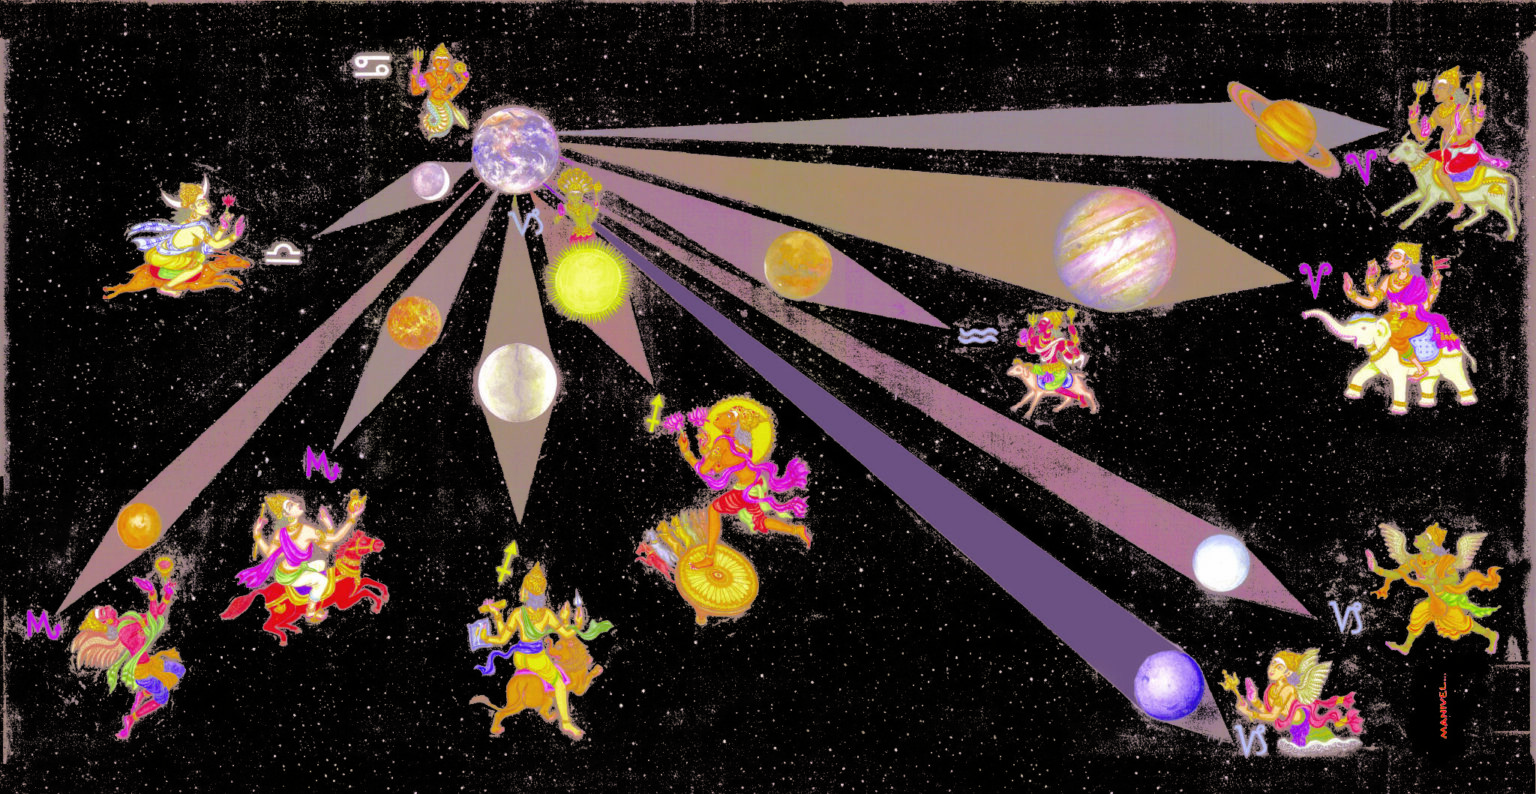
\includegraphics[width=0.8\textwidth]{pics/intro1.png}
\caption{Jyotish}
 \end{figure}

\subsection{BOOKS AND CDS FOR COURSE}
 

Astrology of the Seers: A Comprehensive Guide to Vedic/Hindu Astrology is the main book required for the course,
With Ayurvedic Astrology: Self Healing through the Stars for Part II is also required for the course.
Jyotir Bhava, Vedic astrology Mantra CD of Yogini Shambhavi Chopra (Lotus Press). This is recommended for all students wanting to know the correct pronunciation of the main mantras to the planets. Links to these chants can be found in the course and on the website.
      We generally recommend that the student complete this course material before embarking on an extensive study of traditional Hindu astrological literature, but this is left up to the discretion of the student. Traditional Hindu astrological literature can be cumbersome and without the proper background it is difficult to approach.  However, once the student has grasped the basics of the system, a study of such classics as the Brihat Parashara Hora Shastra, Brihat Samhita and Brihat Jataka (of Varaha Mihira) can be very helpful.  

\subsection{VEDIC SOFTWARE}   Many good software programs in Vedic Astrology exist notably Parashara’s Light. We recommend that the student purchase a good software programs in order to run and study charts on their own. Most software programs provide demos for you to explore and see how they work. The calculations required for Vedic charts is extremely difficult and time-consuming otherwise. There are also now some very inexpensive but more limited programs like Jyotish-D for iPhone and IPad. Note that we do not represent, nor do we receive any payment for any student who orders any Vedic software.


\begin{figure}[H]
 \centering
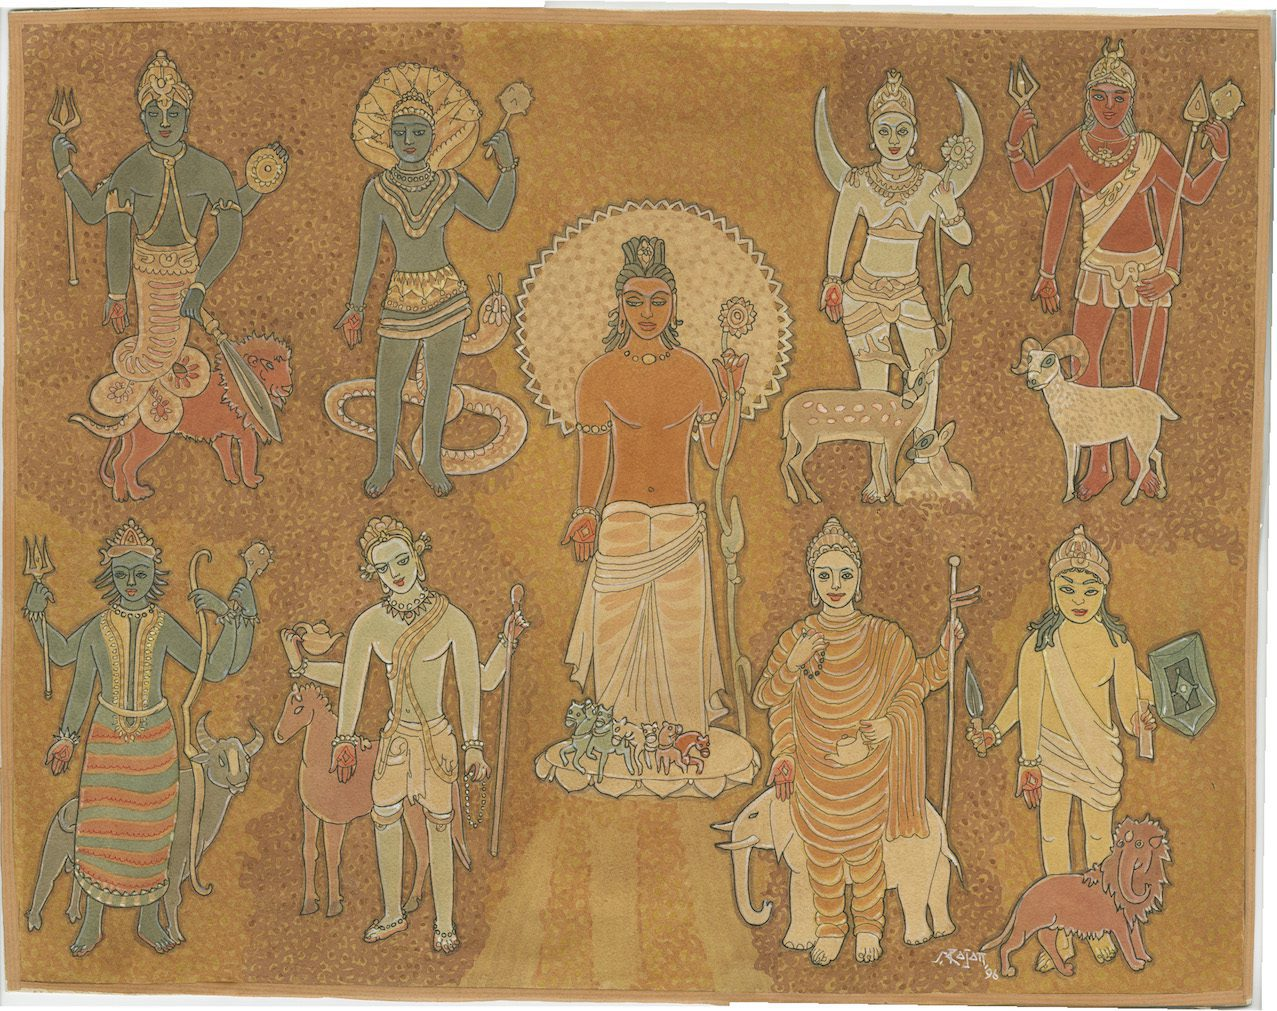
\includegraphics[width=0.8\textwidth]{pics/intro2.png}\caption{Planetary Deities}
 \end{figure}


\subsection{FORMAT OF THE COURSE}
  The course consists of 4 parts:

Part I deals with the main interpretative factors of Vedic Astrology, the foundational material.
Part II deals with Ayurveda, factors of Medical Astrology and remedial measures in Vedic Astrology.
Part III gives specialized, advanced and supplementary material on topics such as Nakshatras, Horary Astrology and Ashtakavarga.
The Workbook stands as a fourth section and is used along with the other booklets starting with Part I, will be noted in the course material.
 
\subsection{Course Workbook}
The Workbook is intended for usage in the following way:

Lessons 1-4 of the Workbook should be examined along with Part I of the course. There will be indications in Part I and at its end about this.
Lessons 5-7 of the Workbook should be examined along with Part II of the course. There will be indications in Part II and at its end about this.
You can examine the appendices in the Workbook at any time as these are for general reference.
  The Workbook is meant to provide technical and practical material, including example charts. It contains study exercises but no questions. However, a few of the questions in the tests at the end of Part I and Part II are based upon the Workbook and cannot be answered without completing it. The Workbook is particularly important for those seeking advanced training in Vedic Astrology. Others may find the Workbook to be challenging. They should be patient and realize that such application is necessary in order to learn to read charts.  

\subsection{COURSE ILLUSTRATIONS}
Course illustrations derive mainly from the Hinduism Today magazine and monastery and are under copyright. Please honor this.   COURSE AUDIOS AND VIDEOS Courses contains numerous audios and several videos to enhance the course material. These are being added to over time.  


 

\subsection{Final Test Questions}
At the end of each of the three main sections are certain Final Test Questions. The student should complete these test questions and send them to the Institute for grading.
Only if these three final tests are answered will the student receive certification for the course.
Course progression percentages are merely book marks of where in the course you have opened to the lessons. These percentages do not indicate actual course completion, which is only indicated by completion of final tests.
You can copy the tests from the on-line course material and add your answers and then send to us by email at vedicinstitute@gmail.com.
Send tests back in Word or Pages attachment. Do not send in PDF or embed in your email. This makes it easier to keep track of your tests.
Please include your name, the date you signed up for the course and your address on the test.
As it is an open book test we expect the student to answer all questions correctly.
You can also ask whatever additional questions about the course material you have along with the tests.
It usually takes us a day or two and up to a week to answer final tests. If you have not heard from us after that, please resend your tests, as sometimes tests do get lost in the spam mail.
 

\subsection{\textbf{SPECIAL AUDIO INTRODUCTION TO THE COURSE BY DR. DAVID FRAWLEY (VAMADEVA SHASTRI)}}
    

\subsection{VEDIC ASTROLOGY READINGS FOR COURSE STUDENTS}
Consultations
Those looking for Vedic astrology consultations can schedule these with Yogini Shambhavi Chopra, Shambhavi.yogini@gmail.com. Shambhavi provides an excellent approach to Vedic counseling through Vedic astrology. For students wishing to have Vedic astrological readings with us, you can arrange a reading with Yogini Shambhavi Devi (shambhavi.yogini@gmail.com), who is our resident Jyotishacharya. Yogini Shambhavi is one of the most respected women Vedic astrologers and Yoga teachers in India and the West.        Such readings can be very helpful in understanding Vedic astrology, as well as how to give readings, but are not included in the course and have their own separate charges.  

\subsection{OUR WEBSITE AND SOCIAL MEDIA}
 

Our web site at WWW.VEDANET.COM contains many articles, publications and resources.
  It includes a listing of books on Ayurveda and other Vedic topics by Dr. Frawley, and a set of over one hundred articles by Dr. Frawley on various aspects of Vedic knowledge, including sections on Ayurveda, Yoga and Vedic astrology. It contains extensive information on Yogini Shambhavi Devi, including her teachings and astrological consultations. Our various programs, intensives and travels are explained in detail. We advise the student to look at these website resources periodically for additional information in the field.  

\subsection{OUR FACEBOOK ACCOUNT FOR AMERICAN INSTITUTE OF VEDIC STUDIES} – for articles, retreats, travels and programs relative to the institute – https://www.facebook.com/americanvedic/
Dr. Frawley’s FACEBOOK ACCOUNT at https://www.facebook.com/drdavidfrawley – Regular information about Dr. Frawley and his many articles, programs and activities in the greater Vedic field, including his work in India, with over a hundred thousand followers. Not specific to Vedic astrology.
Yogini Shambhavi’s FACEBOOK ACCOUNT at https://www.facebook.com/yogini.shambhavi/ – Yogini Shambhavi’s special teachings, information and resources on Shakti Sadhana, Women’s Healing and our Yoga and Ayurveda retreats.
 Dr. Frawley’s TWITTER ACCOUNT at https://twitter.com/davidfrawleyved –  Features Dr. Frawley’s educational and social work in India, with six hundred thousand followers, which includes noted leaders, writers and spiritual teachers. Not specific to Vedic Astrology.
 

\subsection{COURSE REFUNDS AND TERM FOR COMPLETION} For such on-line courses, refund must be requested within thirty days. There will be a $50.00 processing fee taken out of the payment for our time involved. You have up to three years to access and finish the course.  

\subsection{CERTIFICATION}
  Certification for the course is given through THE AMERICAN INSTITUTE OF VEDIC STUDIES. The course provides certification for 300 hours of study in Vedic Astrology (which is how long the course, its exercises and tests, and books should take to complete), and the title AYURVEDIC ASTROLOGER: FOUNDATION COURSE.   As our institute has its own global recognition, this certification has value in its own right, particularly for combining Ayurveda with Vedic Astrology. You can also call yourself a student of Dr. Frawley, who is one of the most respected Vedic teachers in the world today.   Certification in this distance learning course does not mean that you are a fully qualified Vedic Astrologer but that you have a good foundation of information in which to become one. The course is a first stage in training in Vedic Astrology, which usually takes two years in order to become competent in the subject, like any technical discipline or profession. Yet it provides you much useful information to use for the rest of your life.  

\subsection{FURTHER TRAINING OPTIONS WITH US} Additional Programs

This course goes along with our other online courses, Ayurvedic Healing for those who wish to study Ayurveda more deeply, Integral Vedic Counseling for those interested that topic, and Yoga, Ayurveda, Mantra and Meditation for those who wish to integrate the spiritual and psychological aspects of Yoga and Ayurveda.
Dr. Frawley does take on a few students for special advanced training with him personally.
Integral Vedic Master Educator Certification, Ayurveda, Raja Yoga, Vedic Astrology, Vedic Counseling. For select students who have completed all our four courses and want a background recognition of the interconnection of their studies.
For advanced study you may consider more in-depth programs on any of the Vedic Sciences, if you have not studied these, including Yoga, Ayurveda, Vedic Astrology and Vastu. Note our courses in these fields. You might also want to take consultations with various practitioners in these fields. Dr. Frawley takes on a few private students. You can contact us if you are interested in this option. Generally this is limited to those who already have studied, practiced or taught the Vedic teachings for a number of years. It usually requires that you attend some of our retreats as well

Dr. Frawley is available for special Vedic Counseling Sessions that can also help guide you in your Vedic Counseling Practice.
 

May your study and practice of Vedic Astrology prove fruitful, transformative and enlightening! Sri Veda Purushaya Namah! Dr. David Frawley (Pandit Vamadeva Shastri)  

Namaste! 

\subsection{INDIAN NATIONAL TELEVISION (DOOR DARSHAN) INTERVIEW WITH DR. DAVID FRAWLEY}
The link is to aninterview of Dr. Frawley that explores his approach to Vedic knowledge, including Vedic astrology. For those of you who are not familiar with the scope of his work, please view it. It will help you understand the spiritual and philosophical background for this course. With Rajiv Mehrotra, not film maker and associate of the Dalai Lama. You can view it directly here. \url{https://www.youtube.com/watch?v=O0uxv-KBQgA}


\newpage

\section{THE BACKGROUND OF VEDIC ASTROLOGY}
 

The following lesson introduces the student to the background issues of Vedic Astrology and the Vedic way of approaching astrology, applying it, and what the karmas involved may be, both for the client and the astrologer.

 

\subsection{SYSTEMS OF ASTROLOGY – EAST AND WEST}
 

Vedic Astrology is a “sidereal” astrology. This means that it uses the sidereal zodiac or the zodiac of the fixed stars. In this regard, it differs from most Western Astrology, which employs the “tropical zodiac” or the zodiac of the equinoxes. The two zodiacs are currently around 24 degrees apart according to the Ayanamsha used, with the Vedic sidereal zodiac falling behind the tropical zodiac.

 

To put it simply the tropical zodiac always begins the zodiac with the point of the vernal or spring equinox as representing the beginning of the sign Aries. The sidereal zodiac calculated the beginning of the sign Aries from a  certain point in the fixed stars. As the point of the equinox is moving backwards in the zodiac over time, the different between these two systems is now considerable and the calculations of planetary positions relative to them will vary by nearly one sign. While the sidereal zodiac of the fixed stars that Vedic astrology used can be viewed against the actual constellations in the sky, the tropical zodiac is a mathematical abstraction that cannot be seen in the sky as its boundaries are changing over time.

 

In general terms, we refer to Vedic astrology as sidereal and western astrology as tropical as these are the dominant systems. There is, however, a “Western Sidereal Astrology” introduced in the early twentieth century, which uses the sidereal zodiac but otherwise follows the aspects, house orientation and other methods of Western Tropical astrology. This is the basis of the “Fagan-Bradley” system. It arose through the influence of Vedic Sidereal astrolo­gy, but also argues that the original Western Astrology was a sidereal system. We may, therefore, call Vedic Astrology “Eastern Sidereal Astrology” but as Vedic Astrology is a simpler term.

 

There are also a few Vedic astrologers who use Vedic principles relative to the tropical zodiac, or who even claim that the original Vedic zodiac was tropical, but their numbers are very few, and they are not endorsed by the majority astrological community in India.  We find that view to be unfounded and misleading as Vedic texts for thousands of years have pointed out the shifting positions of the equinox and solstice points relative to the fixed stars.

 

In any case, different systems of astrology like different systems of healing are possible, and their principles can be different. Here we are aiming at classical Vedic astrology such as has dominated in India for many centuries and is sidereally based. We are not saying other systems may not have their value. However, there is only one zodiac and we find dividing it according to the fixed stars makes more sense as a way of understanding stellar influences, than dividing it by the equinoxes.

 



 

 

\subsection{THE ASTROLOGER AS LIFE-COUNSELOR}
 

The astrologer functions as a “life-counselor,” able to address all domains of life, including health, psychology, career, relation­ship, and spiritual issues. The field of astrology is the field of life itself. There is probably no other field that has such a broad scope of applications. The astrologer can specialize in one area but needs to know something of the whole of life. Astrol­ogy shows us the basic energetics of our lives in all their different dimensions. Some astrologers may take more limited roles or simply aim at providing information, not advice. But we feel that the life-counselor model is more useful and a better basis for practice, particularly in the West.

 

To be an astrologer, therefore, can be a more holistic career than to be a  psychologist or therapist of any kind. It requires a breadth of view and capacity to contemplate life as a whole. It may be the ultimate holistic occupation. To really do Vedic Astrology requires an integral approach and pyramidal vision, such as is revealed in the system of Vedic Science that covers all aspects of life. The astrologer should guide his or her client through the domains of life toward the full unfoldment of the soul, not through giving rigid directions or predictions but through pointing out the full scope of the clients potentials along with practical tools for developing their energies properly.

 

The astrologer should therefore study Yoga, Ayurveda and related Vedic subjects in order to be competent in this comprehensive approach. It is not necessary to master all of these subjects before attempting astrological readings, but one should gradually learn their fundamentals. Some astrologers possess much knowledge intuitively. Others bring it forward from different kinds of learning that they have already done.

 

Good astrological knowledge itself may not be enough to be a good astrologer. Just because we can see how the stars affect people or when events may occur in their lives, this may not be enough to help them understand these events or use them properly. There may be those who are good astrologers in some way or another. They may have good predictive powers but they may be unable to guide anyone in the higher goals of life. This requires not only astrological knowledge but spiritual development and integrity. A Vedic Astrologer should themselves follow a spiritual discipline, practicing yoga, meditation, mantra or rituals daily, and leading a life of honesty and integrity.  Their aim should not be to seek wealth, fame or power but to be of genuine service to their clients.

 

\subsection{THREE MODELS OF VEDIC ASTROLOGY}
 

Several different models of astrology exist. Two commonly related methods in Vedic Astrology today are the “predictive” and “judgmental” systems. Some people identify Vedic Astrology with these as a rigid and deterministic system. This is a misunderstanding. Vedic Astrology is also a very important counseling system, though it does have its predictive value.

 

\subsubsection{1. PREDICTIVE ASTROLOGY}
 

Predictive astrology aims at predicting specific events in life. These are mainly mundane events such as the timing of marriage, birth of children, the time of death, onset of various diseases, accidents, financial gains or losses, times of good or bad fortune, even the times of renunciation or liberation on a spiritual level.

 

The predictive astrologer aims at being able to predict events as specifically as possible. To this end, he may use not only the birthchart but also divisional and horary charts. These predictions may extend into the world at large, predicting wars, earthquakes, election outcomes, economic trends, stock market activity and even the weather, which are all part of mundane astrology.

 

Predictive astrology is linked to the timing of events. It is concerned with planetary periods, progressed charts, transits, horary charts and electional astrology, where timing is most important. It studies how outer events reflect astrological patterns and predicts the timing of their fructification.

 

From the standpoint of predictive astrology, the skill of the astrologer is judged by the accuracy of his or her predictions. The astrologer becomes a kind of weatherman for astral influences in life. There is not always something spiritual about such skill, but it can be allied with deeper insight. Such knowledge does not necessarily show us how to rightly deal with these events in our lives, although it can be combined with that as well.

 

From the standpoint of Vedic Astrology, predictive ability is important in an astrologer and it is a skill that all Vedic astrologers should strive to develop. If we cannot determine the astrological influences behind the events of a person’s life, we may not be able to determine how they affect them at a deeper level. Such outer events allow us to verify the chart and reflect the accuracy of our chart interpretations. This does not mean that we must always be able to tell our clients when specific things will occur to them on a daily basis but that at least we should be able to show them the major trends of their lives. Actually predicting specific events in the future is very difficult and has its dangers as we may be interfering with a person’s own power of judgment.

 

The predictive side of Vedic Astrology is probably the best of any astrological system and affords it much value. Many people approach it for this alone, particularly people from India who have a more uncertain material life. But it should be used to help clients put the events of their lives in proper perspective, integrating it into a spiritual approach that shows them how to use these events for spiritual development. It should not degenerate in giving the person the view that their life is mapped out or that they are victims of fate. In addition, until one has spent many hours examining a person’s chart and subchart it is not possible to understand the short term trends and indications in the chart. A mere general life-reading cannot do this.

 

 

\subsubsection{2. JUDGMENTAL ASTROLOGY}
 

This form of astrology aims at judging the different aspects of the life and character of a person: Their health, longevity, career, finances, marital happiness, level of intelligence, stage of spiritual evolution, and so on. It is similar to the predictive method, but looks to general capacities rather than to specific events. Most importantly, it has an ethical or spiritual side that some people are sensitive about. Many people do not like to think that they can be judged from a chart or that there is any limitation to their fate or destiny. However, Vedic Astrology, with its karmic orientation, acknowledges the history of the soul and the opportunities and limitations of each person and integrates this insight into its system.

 

Judgmental astrology places a value judgment on astrological positions. Some aspects are said to be good or bad, some planetary combinations are said to make a person good or evil, or intelligent or stupid. It often has an implied moralism that we should be very careful about, as karma is full of mystery and different indications.

 

Astrology should be capable of providing helpful judgments in life. But these should not be simplistic or subjective. They should be based upon spiritual goals and should not exalt worldly success or outward happiness as being of ultimate value. For example, a chart may indicate disease. This, however, is not necessarily something bad. It does not necessarily mean that person did something evil in their last life for which they have to pay. Disease can be an important means of awakening the soul. Therefore judgments in astrology should be applied with discretion. While astrologically we can see trends and tendencies, we should never deny the freedom of the soul to awaken and transcend its karma inwardly, even when it cannot change it outwardly.

 

Both the Predictive and the Judgmental models of astrology can have a fatalistic note about them that inhibits taking control of our own lives. Predictive astrology tells what is going to happen to us, as if we had no free will in life. Judgmental astrology tells what our nature is, as if nothing could be done about it. If we apply them in too matter of fact a way, we will encourage a fatalistic attitude in our clients. They will take their good fortune or misfortune too seriously, with finality, and lose the capacity for creative and spiritual growth in life. They may feel insulted or degraded by negative judgments and predictions, or flattered by the positive ones. Neither response leads to right action in life.

 

This fatalism occurred in medieval Western Astrology that also was judgmental in nature.  It was linked to a culture that believed in the predestination of the soul, and in an eternal heaven and hell. Such fatalism cannot exist in the Vedic system which is based on karma. Karma is not fate or predestination. It is a law of cause and effect in which our present state is the result of our past actions. We create our own destiny but we do so through time, in which who we are today has already been shaped by what we did yesterday.

 

Vedic Astrology does recognize the limitations of past karma, which can be very difficult to overcome, but it also teaches us that we can change our future. The future is the result of present actions, just as the present is the result of past actions. Vedic Astrology therefore encourages individual effort, not passivity, which is why remedial measures are so important. That past actions have influenced our present state does not mean that we should just accept our condition as limited. It means that we should act in a way today so as to ensure a better future and a more positive forward movement of our karma.

 

This course does not limit itself to Predictive or Judgmental methods, though they are used within it. The Predictive method, if applied superficially, becomes too mundane in nature. It can turn the astrologer into a mere fortune-teller. It gives people the impression that their destiny in life is fixed and that a good astrologer can remove any mystery about what will happen to them.

 

We should add that prediction is easier in a fixed and traditional culture like India. In the modern West, many of these predictive rules fail. For example, the potential for divorce is much higher in western culture today. For this reason, the traditional Hindu rules of marriage do not always work on charts of people in the West. Hence, these rules must be altered. They can show ease or difficulty in relationship, but how that translates into marriage or divorce is conditioned by the time and by the culture.

 

The Judgmental method can be too harsh. It can deprive people of the capacity for growth. It can reinforce any negativity in the chart. Even if the outer chart has many weaknesses, it should never be forgotten that our inner Self and true Being inherently transcends the influences of time and space. This method is particularly dangerous with passive, self-negative types of people who easily believe what is told to them, and are ready to accept something negative about themselves. It often becomes a self-fulfilling prophecy.

 

Personally, I think there is undesirable karma in following these methods too strongly or rigidly. To tell a gullible person that they have certain limitations in life or that they will suffer some difficulty at a certain time may make it occur. The astrologer should act in such a way as not to deprive the client of his or her own power of judgment. The astrologer can give clients information or tools to work with but they must not take power over their clients. The astrologer is not God and the birthchart is seldom so fixed that all astrologers will interpret it in the same way. Therefore, the astrologer should not be too proud or convinced of his or her opinions. He should remain open to the fluidity of life. While we may have to warn our clients of the effects of wrong actions, this should stimulate them to a better way of living, not make them feel that they cannot change their condition.

 

There is yet another approach to Vedic Astrology that we should note. This is more the flattery method in which the astrologer tells the client everything good about them and their chart. It may be done in an effort to show people the positive side of their nature or it may just be done to gain more clients. If we do not point out the difficulties inherent in a chart, we are also doing our client a disservice. We should point these out in a way that enables the client to use them as a basis for greater growth and understanding. We should neither ignore them nor present them in a rigid manner. We should point out both the positive and the negative objectively and try to give the client the tools to use the higher potentials in their chart – and there is seldom a chart without them.

 

\subsubsection{3. SPIRITUAL ASTROLOGY AND ASTROLOGICAL COUNSELING}
 

The system taught in this course is more a form of spiritual astrology and astrological counseling. It uses astrology as a tool for self-knowledge and an aid in Self-realization. It uses the cosmic forces transmitted to us through the planets to connect us with our own deeper cosmic nature. In this regard, I always teach my clients the basic meaning of the planets in their charts and the characteristics of their planetary type. This allows them to enter into the process of astrological knowledge which is necessary for astrology to become a useful tool for self-growth.

 

It employs predictive and judgmental methods but in a broader spiritual context. I try to acquaint my clients with both the good and bad potentials of their chart and offer them the tools to augment the good and ward off the bad. I do not leave my clients victims of fate. I teach them that their soul transcends time and that it can use the energetics of the chart in several ways. I do not recognize an absolute fate in life but only probabilities that can be high, medium or low.  For example, I may tell a client their chart is not good for relationship or that it may be prone toward divorce, but I would be hesitant to tell them that marriage is impossible (though there are cases of this). I would hesitate to give a person the date of their divorce when a difficult period for marriage is indicated. However, I would inform them if a relationship were unlikely to endure through a given planetary period.

 

This approach does not aim at prediction alone. I am more concerned with helping the client to manage their planetary energies rather than merely telling them what is likely to befall them for good or ill. I relate to them favorable or unfavorable periods for different ventures or affairs and help them guide the course of their lives through these. I encourage them to action on all levels through the remedial measures of Vedic Astrology and its related systems of Yoga and Ayurveda. I believe that the proof of a good astrologer is how he or she makes their clients aware of their astral influences and how to better manage them, not how good he or she is at predicting particular events only. Such an approach is not aimed at making the individual more tied to his external nature but opens up the potentials of the spiritual life which the individual may not yet be using or even be aware of.

 

\subsection{THE ASTROLOGY OF HEALING/ YOGIC ASTROLOGY AND AYURVEDIC ASTROLOGY}

 

Astrology requires a healing method to be really useful. We must not only be able to recognize planetary influences in our lives; we need to know how to harmonize them. We must help our clients learn how to balance the planetary influences in their lives.

 

An astrology of healing has two levels: First, Vedic astrology has measures to treat our outer nature and, second, those to treat our inner nature. The outer nature, our body, senses and conditioned mind, can be treated by medical and psychological methods that are not specifically astrological in nature. Our inner nature, our soul, requires occult and yogic methods and ultimately rests upon our own effort to grow spiritually in life. This has more scope for astrological healing measures.

 

Vedic Astrology is not just a predictive or interpretative system.  It is also a remedial system with techniques and methods for balancing planetary influences. These are as essential as the interpretative side. What use is it to tell people what is going to happen to them if we cannot give them a means of dealing with it? For this reason, the second part of this course includes such remedial measures as gems, mantras, yantras, herbs, and color therapy, and the role of Ayurveda as well as Yoga.

 


\subsection{THE FOUR AIMS OF LIFE}
 

On this foundation of examining the different models and goals for Vedic astrology we will now introduce the Vedic view of life. Vedic Science traditionally recognizes four legitimate aims or goals of human life: Dharma, Artha, Kama and Moksha.

 

DHARMA means “principle or law” and refers to the fulfill­ment of our right purpose in life.  It includes the honor or recognition we attain through our actions on a personal and professional level, specifically through the medium of career. It relates to broader principles of truth and right action. Ultimately it refers to our soul’s purpose in this incarnation.
ARTHA means “achievement of goals” and relates specifically to the acquisition of material resources required to fulfill ones dharma in life.  It relates to income and wealth.
KAMA means literally “desire” and refers to our need for emotional and sensory happiness. As such, we could call it “enjoyment.” But lasting happiness is only possible when we fulfill our dharma.
MOKSHA means “freedom” or liberation and relates to our need for spiritual growth, including transcendence of the above three lower values.
 

Vedic Astrology recognizes the validity of all four aims and is oriented to facilitate the human being in the attainment of each of them. Yet in Vedic Science the first three, career, wealth and enjoyment are subordinate to the last, spiritual liberation. Liberation is the primary and essential goal for all human beings. Without it, the other goals have no real meaning. The others are merely a support for it and have no validity in themselves. An astrologer using the Vedic system should, therefore, give a comprehensive view of all the domains of life. Yet he should focus on liberation and the spiritual life. This does not mean to take the role of a guru but to show the higher usages that can be made of the planetary energies and circumstances in ones life.

 

From the Vedic perspective, a chart that is good for liberation but not for the other domains of life is a much better chart to have than one that is good for the lesser goals but not for the spiritual life.

 

As a foundation for the four aims of life, astrology addresses the need for health, arogya, or freedom from disease. This is the basis for the four aims of life, for without health, what else can be accompli­shed? Yet health is not just physical, it is also mental. So astrology must consider physical and mental health or physical health and psychological well‑being as the means of approaching all the goals of life. Hence, medical and psychological astrology, after spiritual astrology, are its most important branches.

 

I have addressed some of the astrological indications of these factors. These will be more understandable later on in the course.

 

 

\subsubsection{DHARMA}

 

Dharma refers in a broader sense to the spiritual principles and natural laws that govern the universe. In the individual context it refers to our basic nature, inclinations and capacities in life. Dharma as career, refers to right vocation and the happiness inherent in fulfilling ones capacities for right action in life. Ones true Dharma is that of ones soul, our hearts vocation, not what society imposes upon us. Yet most of what we call Dharma is revealed by our occupation in life, how we earn our livelihood.

 

Under this concept are also included honor, position, status, fame, prestige and power. These show our social dharma and its effects, including how our character affects the world. Our individual dharma should reflect in some way the universal dharma. If our dharma is adharmic; that is, if our career is harmful to others, then it will end up harming ourselves as well.

 

Dharma is related to Artha, the objects and goals that we seek to attain things in life. Usually it is through our career that we seek wealth.

 

 

\subsubsubsection{Indications in the Chart}

 

These indications will make more sense later in the course after students are more familiar with the planets. Please remember it for future reference.

 

Jupiter, Mercury and the Sun are the main planets that rule Dharma. Mercury shows how we function and communicate in society. Jupiter shows the role or law we like to follow in life, our guiding principles and the goals we seek. The Sun shows our ability to project our character and personality, the influence of our nature on the world.

 

Dharma houses are the first, which shows our personal dharma and responsibility to self, the fifth which shows our creative dharma and responsibility to children, and the ninth that shows our spiritual and social dharma.

 

For house influences, we should note that of the first, ninth and tenth houses and their lords. The first tells us who we are generally; it is the measure of our identity and action in the world. The ninth shows the goals or profession we aspire to. The tenth measures our capacity to impact the world karmically. It shows how our personality appears in the world. It shows how our dharma achieves artha, or value, both for ourselves and for society.

 

 

\subsubsection{ARTHA}

 

Artha, wealth, refers to all necessary means of material livelihood and security, not simply the pursuit of material gain. The astrologer should be able to counsel his clients on how to best use their material potential in life. This is in directing it towards spiritual or dharmic ends, not simply pursuing money for the power or status that it may afford.

 

 

\subsubsubsection{Indications in the Chart}

 

The planets that rule Artha are Jupiter and Mercury. Jupiter governs our capacity for gains and abundance generally. Mercury rules our ability for commerce and exchange. Venus also gives wealth and comfort, art or luxury. Saturn tends to create poverty (though it can give us property and other hard or fixed assets).

 

Houses of artha are the second, sixth and tenth. The second shows how we gain our personal livelihood. The sixth shows work capacity and money from sources such as insurance or legal settlements. The tenth shows career gains, staus and achievement.

 

In particular, we should take into account the influences on the second and eleventh houses and their lords. The second governs our ability to earn through our own labor, the eleventh to gain income from various sources. After these we should consider the fourth, fifth and ninth houses and their lords, which all give wealth. The fourth gives property and vehicles. The fifth gives gain through counseling, advice and speculation, like the stock market. The ninth gives grace and fortune, like the winning of lotteries.

 

The twelfth, sixth and eighth houses and their rulers tend to limit wealth. The twelfth shows loss and expenses. This in itself may not create poverty if the houses of income are strong. The sixth gives loss through disease, enmity, legal problems, overwork or lack of recognition. The eighth shows difficulties, obstacles, oppression, lack of recognition or bad reputation.

 

 

\subsubsection{KAMA}

 

Kama, enjoyment, refers to all legitimate sensory enjoyments, not just pleasure in the gross sense but the enjoyments natural to the right use of the senses. To enjoy life, to appreciate the beauty of nature, true art and loving communication between human beings, is part of the fulfillment of our soul and need not be denied for spiritual growth. In fact, all life is a seeking of happiness. It springs from joy itself. If we were not in some way happy or able to find happiness, why would we wish continue living?

 

Our enjoy­ment or pleasure in life is largely through relationship, which includes sexuality. Hence, relationship is the main factor of Kama and its issues of love, marriage, partnership and children. The higher level of Kama or enjoyment relates to our artistic sense. The highest level relates to our capacity for devotion, our openness to Divine love, beauty and delight.

 

 

\subsubsubsection{Indications in the Chart}

 

The planet that rules Kama is Venus, the planet of desire. According to its position in the chart, our capacity for enjoyment or Kama can be read. Mars is also important as it shows our goal-seeking in life. Aligned to Venus, it often takes us along the realm of desire. Jupiter gives us capacity for enjoyment or happiness of a more general nature, while Saturn tends to deny or limit it. Saturn aligned with Mars may cause us to seek perverted or unwholesome means of enjoyment.

 

Kama houses are three, seven and eleven. The third is the house of talents, hobbies, curiosities, interests and sports – personal kama. The seventh house is the house of love, marriage and fulfillment in human relationship – relationship kama. The eleventh is the house of friendship, expression, social and career gains – social kama. The fifth is also important as the house of romance, joy and creativity, the happiness that comes from dharma. The twelfth is the house of secret pleasures and hidden desires and has some relevance as well and also indicates the happiness that comes from moksha.

 

 

\subsubsection{MOKSHA}

 

Moksha, liberation, refers to our work of Self‑realization in life, our efforts at Self‑knowledge. It includes whatever liberates our inner spirit and creative force in life. In its proper domain, it transcends organized religion and codified beliefs and is ultimately an individual affair.

 

The pursuit of various forms of knowledge, including philosophy, science and the occult, as well as creative expression, like art, are themselves lesser aspects of the goal of liberation. For this reason, the aim of liberation can also be defined as knowledge. All of us are seeking knowledge or freedom in one way or another. It is knowledge that gives us freedom, which extends our horizons and gives us access to the greater world beyond the limits of our body and senses. Yet knowledge may be lower, as of the outer world, or higher, as of the true Self. This latter is the real goal through which real liberation is possible. The lesser knowledge gives us greater space to operate in the world but it does not free us from the limitations of worldly existence.

 

 

\subsubsubsection{Indications in the Chart}

 

Jupiter and Ketu rule Moksha. Jupiter shows our general seeking of expansion and truth, our aspiration and need to grow and transcend. Ketu shows our ability to negate and transcend things. It affords deep insight, discrimination and perception. Saturn is also important as it gives detachment, renunciation and the capacity to be alone. Mercury is important, as the indicator of the intellect; it shows the level of knowledge that we seek.

 

Houses of Moksha are fourth, eighth and twelfth. The fourth shows our emotional happiness. The eighth shows occult and mental insight. The twelfth shows spiritual liberation.

 

The house influences of the ninth and twelfth together are important, as well as their lords, with Jupiter the significator of the ninth and Ketu of the twelfth. The ninth gives us our sense of values, goals, principles and aspirations. It shows the dharma behind our pursuit of moksha. The twelfth allows us to negate our experiences and go beyond what we already are (our conditioned being). It also shows the past and the latent impressions in the subconscious that motivates us. The fifth house has some importance as the measure of the good karma we bring into the present life, the indication of past spiritual practices. It also shows our devotion in life, what form or energy of the Divine that we seek.

 

The fourth and eighth houses also relate to liberation. The fourth shows our capacity for peace of mind, the foundation of all spiritual pursuits. It shows self-contentment, psychological stability and mental receptivity. The eighth shows our ability to go beyond death and time, the gateway to the eternal. It gives the ability to transcend suffering and often affords deep perception.

 

The planets of ignorance and attachment often limit our pursuit of Moksha. These are particularly Venus and Mars, the planets of passion and sexuality. Saturn can provide the detachment that aids us in liberation or it can create darkness of mind that prevents it. Jupiter can get us attached to outer affluence or religious ceremonialism. Hence, liberation is the most complex thing to measure in a chart. All planets have a higher or spiritual and lower or materialistic functioning.

 

Jupiter, as the great benefic, is the planetary indicator of our positive goals in life. So it is the most important planet in showing how we can achieve any of the four aims of life. How our Jupiter is oriented will show the areas in which we will seek our highest good in life.

 

Saturn, as the indicator of karma or destiny, shows the limitations we encounter but is also useful in giving us the lesson of suffer­ing that takes us from the lower to the higher goals.

 

When both Jupiter and Saturn balance each other and further spiritual knowledge, we are able to attain our maximum destiny in life and become a person of true greatness.

 

The lunar nodes have a similar importance. Rahu, the north node, shows where we are apt to overly project ourselves into the outer world. Ketu, the south node, indicates where we are prone to overly contract ourselves into the inner world. When the lords of both nodes are in harmony our lives function well. When they are in harmony on a spiritual level, great transformation is possible.

 

\subsubsection{Relationship between the Four Aims of Life}

 

These four aims are like a pyramid with liberation at the top. Each is meant to aid in the others. We need to be happy generally in order to function at all. We need the resources to enable us to have leisure and peace of mind. We need the acknowledgment or recognition of others. In this regard, a failure or inability to achieve the lower goals can inhibit the higher. If we are impoverished, degraded, ill or stupid, it is difficult to get beyond the outer aspects of life.

 

Yet most of us are caught in the lower goals and do not appreciate the higher in our true nature. Often our pursuit of the higher remains a pursuit of the lower in disguise. In the name of God, we still seek pleasure, power or fame. Astrology is also usually denigrated in such a way when its lower rather than higher insights are implemented.

 

It is important not to deny the pursuit of any of these aims for anyone but to show how they relate properly to and direct us toward the true goal of spiritual liberation. We should never encourage a client to pursue these outer goals as the highest pursuit in life. There may be times in life when it is necessary to focus on them or take advantage of the favorableness of the time to achieve them, but this can be done with a long-term spiritual orientation. For this reason, we should not give the lower goals too much weight in reading a chart. A purely business astrology, for example, would not be in harmony with the Vedic approach unless the business was oriented towards spiritual goals.

 

When we define success or failure, difficulty or ease for people based upon their charts, we must indicate in which domain and on what level. We may judge a chart as good for wealth or career, but this does not mean it is good for health or spirituality. In this way, many charts that are difficult for ordinary goals have higher blessings.

 

\subsubsection{THE KARMA OF AN ASTROLOGER}

 

The modern world does not believe in karma, but in money and the fame that the world gives us. There is the tendency to think that if our work gives us wealth and recognition then it is good. This, however, may not be the case. As wealth and recognition are outer values, they can come to us according to an outer or unspiritual orientation in life. Astrology can give wealth and fame but also deeper knowledge. The two are neither inclusive or exclusive of each other but the latter is the real grace of astrology through which alone true happiness will come to us.

 

To do Vedic Astrology properly, we must teach our clients the laws of karma and live according to them ourselves as well. Vedic astrology is the ultimate system of karmic management, both for ourselves and others. It is not our name and wealth that we take with us when we die but our karma. It is our main purpose in life to reduce our karmic burden and aid others in doing so. This is also the true role of the astrologer. A worldly astrology that flatters people, that encourages them to seek happiness in the outer world, that glorifies wealth, fame and talent, breeds more karma for the astrologer and their clients.

 

As astrology is an intimate form of counseling and deals with the deepest issues of life, it carries great responsibility. It has a power that can work against us if we apply it in the wrong manner. If we give our clients wrong advice or project them in a direction that may not be helpful to their soul, then it will be our karma to similarly be misdirected by others or to misdirect ourselves. Even if a chart is very good for outer things like wealth, we should not simply glorify such good fortune for our client but show its limitations. Similarly, if a chart is not good for the outer goals of life, we should point the positive value of such a chart for bringing us into the spiritual life.

 


\subsection{\textbf{Talk by Dr. David Frawley on Vedic Astrology and Vedic Counseling
Shows how we view and apply Vedic astrology in our integral approach to Vedic knowledge}}

\begin{figure}[H]
 \centering
\includegraphics[width=0.8\textwidth]{pics/overview1.png}
 \end{figure}

\begin{figure}[H]
 \centering
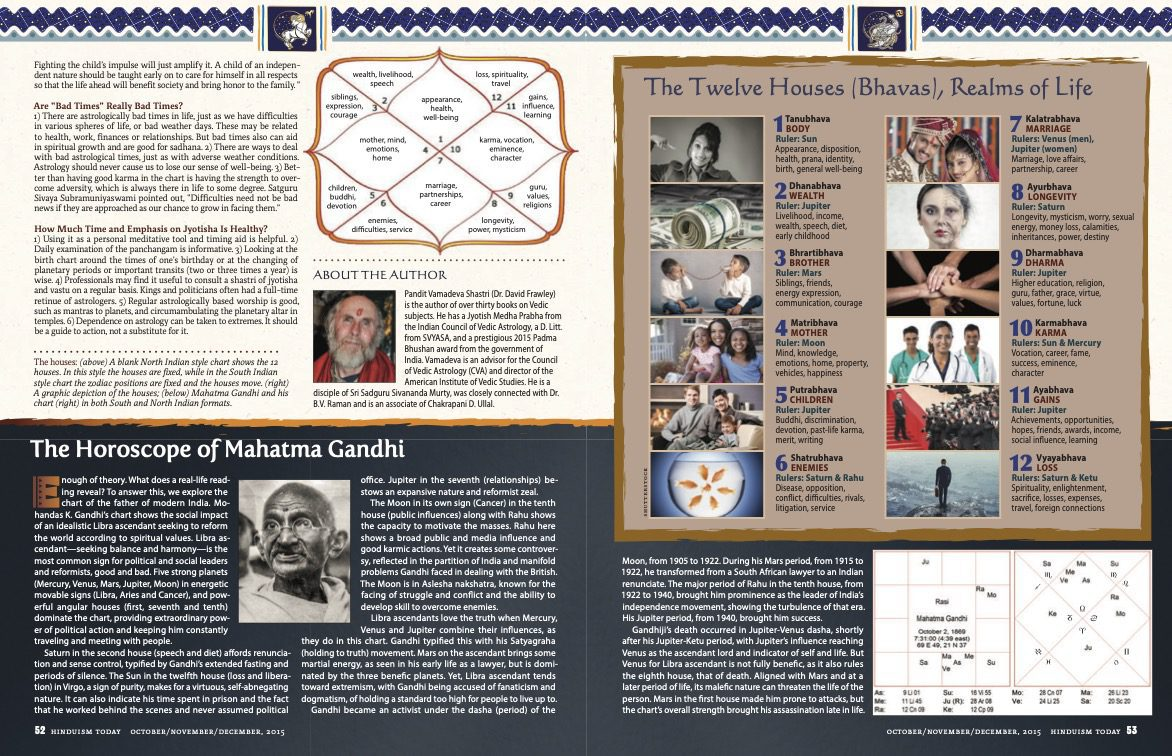
\includegraphics[width=0.8\textwidth]{pics/overview2.png}
 \end{figure}


\newpage

\section{OVERVIEW OF VEDIC ASTROLOGY}
 

This lesson is based upon a special feature issue on Hindu/Vedic astrology that Vamadeva did for the magazine Hinduism Today some years ago. It addresses the practical questions about Vedic/Hindu astrology and its applications. It does not deal with the technicalities of reading a chart that we will examine later in the course. It addresses the background, role and usage of Vedic astrology overall, and how to explain its relevance to a general audience and their concerns about its nature, validity and usage. We have recently edited and updated this lesson.

 



\subsection{EDUCATIONAL INSIGHT}
Jyotisha, Hindu/Vedic Astrology

How the Science of Light Can Help You in Daily Life

By Pandit Vamadeva Shastri

 

In the Hindu view, the planets are not mere celestial bodies circling the Sun. They are also divine beings. Each is like a prism, conveying subtle energy from the far galaxies, thus impacting man’s affairs on Earth according to its unique nature and location in the sky. The ancient science of space and time that understands and maps this influence is called jyotisha (literally “science of light”) or Hindu astrology. 

 

It’s About Time

\subsection{AN INTRODUCTION BY HINDUISM TODAY}

Believing nothing, the skeptic is blind; believing everything, the naif is lame. Somewhere between the two lies the lauded land of viveka, discrimination, which neither doubts every inexplicable phenomenon nor swallows every unexamined statement. In this issue we explore the uncanny Vedic technology of jyotisha, that hoary knowledge, derived from secondary Vedic texts, which embraces both astronomy and astrology. It’s about time.

 

President Ronald Reagan confounded the White House staff and embarrassed aides by having his itinerary and major meetings scheduled in consultation with his wife’s astrologer in California. Scoffing staffers counted it pure silliness; others thought it merely impolitic of him, maybe because of the implication that he wasn’t totally in charge or that a Christian would so publicly propound such things.

 

Mr. Reagan is not a lone heretic. Queen Elizabeth I, a Virgo, consulted the stars. Galileo, the Italian mathematician and astronomer, cast charts on the side, as did the German celestial scientist Johannes Kepler. Britain’s Princess Diane followed the stars, and many Hollywood stars do the same. Ditto with Carl Jung and American millionaire J.P. Morgan. A 2013 Harris Poll concluded that 29 percent of Americans (and nearly half of 18- to 24-year-olds) believe in or follow astrology. By contrast, 92 percent of the Chinese public think horoscopes are nonsense.

 

Like so many other things, astrology in the West is about personal things—about me and mine, my spiritual progress, my love life and business success. These concerns are not absent in the East, but larger concerns dominate. Astrology in India is about auspiciousness, about connections, about sacred timing and being in a flow with the ebb and tide of divine forces.

 

Astrology is a part of Vedic self-understanding. We look to the stars to see ourselves better, to discover the mysteries that lie all about us and within us. In rita dharma, that heavenly cosmic orderliness, stars are more than massive conglomerates of molecules or fiery furnaces fleeting afar. They are entities, potent presences that affect us despite their distance. There are, of course, many Hindus today who pooh-pooh such notions. “Stuff and nonsense,” they will cry, “What thoughtful person can accept that stars, so remote, influence life on Earth?”

 

But what thoughtful person, asks the astrologer, would deny the powerful tides dragged across our planet by a faraway moon, or gainsay the not-so-subtle solar forces that are the very stuff of life here? “Ah, but go out another few thousand light years and tell us what petty influences persist,” our doubter might challenge. The jyotishi (Vedic astrologer), realizing the basic East/West difference in world views, attempts to help the skeptic understand the Hindu perspective. “In Eastern thought, particularly Hinduism, we conceive of all existence—including the stars and planets—not as being ‘out there,’ but rather ‘in here’—within the consciousness of each one of us. In other words, consciousness encompasses all of creation. The ‘outside’ and ‘inside’ are mirror images, and the essential nature of the cosmos is not that of multitudinous distinctions but rather the many-faceted expression of a one unified Reality. Thus we do not follow the mechanistic, externalized approach typical of Western thought.”

 

The astrologer is something of a tribal shaman. Ideally, he or she is the one among us with special insight, with a wider vision that lifts awareness beyond our little world, connecting us to the canopy above, expanding perception beyond the narrow sliver of time in which we live by bringing past lives and actions into the now. You could say that astrologers tell time with a bigger watch.

 

The genuine astrologer is, in a sense, a time navigator. He teaches that time is not all colorless and neutral, the same in all directions. Time has its eddies, its waxing and waning, its preferential ways—and in that sense is much like the oceans. No ship’s captain worth his hardtack would consider the sea a uniform body of water, everywhere equal and indifferent to his passage. No, the sea is alive with idle doldrums and treacherous tempests, and, yes, dangers worthy of anticipation.

 

To the astrologer, time is like that sea, with moods and forces, some propelling us swiftly forward, others opposing our well-plotted progress. How foolhardy the seaman who keeps his canvas unfurled in a storm or stows his sails when the good winds blow. Time is a kind of moral wind, blowing now this way, now that. As a ship’s captain heeds the chart reckoned by his navigator as to course, winds and tides, so our life’s journey benefits from periodically examining another chart, our astrologer’s appraisal of protean time’s patterned flow.

 

Those who still doubt are members of a hoary club. Yogaswami of Jaffna had the perfect prescription for them, one that sets aside all of the good versus bad, will versus fate: “All times are auspicious for the pure Siva bhakta.”

 

\subsection{Working with Our Karmic Code}

Philosophically, Hindu astrology reflects the law of karma, which includes both free will and an aspect of predetermination, or fate. Predetermination means our present condition is the result of our past actions from previous lives; free will means we shape our future by our present actions—how we respond to the challenges. The birth chart represents a person’s karmic code, the samskaras with which he or she is born, imprinted on the subtle or astral body. This code is analogous to the genetic code that outlines the main potentials of the physical body. The birth chart indicates the main potentials of our entire life.

 

From an astrologer’s point of view, the birth chart is the most important document we have in life. Yet, like the genetic code, it is written in a mathematical language that requires decoding by a trained expert, and it calls for careful examination over time to unfold its dynamic secrets. K.N. Rao observed, “A horoscope reflects the allotment of karmas of previous lives. We are all getting the results of our karma, but not all of our karma.”

 

According to the Vedas, when a soul takes birth, it descends through the heavens and the atmosphere before reaching Earth, taking on heavier sheaths of material density. It can only take birth in the physical plane at a time karmically in accord with its nature and destiny. The birth chart represents the seed pattern of its life; how it develops depends upon environment as well.

 

Satguru Sivaya Subramuniyaswami advised: “When unfavorable times arise which have to be lived through (as they all too frequently do), we do not carp or cringe, but look at these as most excellent periods for meditation and sadhana rather than worldly activities. Just the reverse for the positive periods. Spiritual progress can be made during both periods. Both negative and positive times are, in fact, positive when used wisely. A competent jyotisha shastri (Vedic astrologer) is of help in forecasting the future as to when times will come along when advancements can be made. A positive mental attitude should be held during all the ups and downs that are predicated to happen. Be as the traveler in a 747 jet, flying high over the cities, rather than a pedestrian wandering the streets below.”

 

\subsection{Cosmic Consciousness}

Astrology is the science of fathoming the influence of the sun, moon, planets and stars upon living creatures. In Sanskrit it is called jyotisha, which means the “science of light”—specifically, “Vedanga Jyotisha,” the astrological limb of the Vedas, said to be the very eye of the Vedas.

 

Jyotisha is a system of understanding how our lives and our karmas relate to the movements of the cosmos, which is cognized as a single greater organism. Under jyotisha is included astronomy, meteorology and forms of divination, including palmistry, the reading of omens, svara (reading the breath) and various oracles.

 

Like yoga, jyotisha is a super science that links us with the cosmic intelligence behind nature. Its first message is that we are one with the Universal Being. New discoveries in quantum physics demonstrate the interrelatedness of the universe, showing subtle levels of immediate interaction even at great distances of time and space. Jyotisha is an integral aspect of the traditional Vedic sciences, along with ayurveda, vastu and yoga, all of which are usually used together.

 

How can the stars and planets influence events on Earth? Obviously the Sun is the basis of all life. According to the Vedas, it also projects a force of intelligence and spirituality. The Moon is important to all creatures and governs the fertility cycles of animals. In the Vedic system it rules the emotional nature. It is well known that the large magnetic and gravitational fields of the planets affect the Earth physically. That they would have subtler influences as well is not illogical.

 

Astrology is common in one form or another in all cultures, though in India it has had the widest and freest development, from the most ancient period to the present day. Ancient Greece and Rome used astrology extensively, as did Europe to the eighteenth century, even though it was often banned by the church. We could say that the type of astrology used by a culture reflects its understanding of the universe, particularly the subtle and spiritual influences guiding our lives. Curiously, modern cultures continue to employ astrology even when its validity is questioned by the scientific community. The ever-popular sun signs in newspapers reveal this undying interest.

 

Jyotisha remains an important facet of Hindu spiritual, religious and social practice, not only in India but worldwide, throughout the Hindu diaspora. It is widely used by Hindus, from common villagers to the sophisticated urban elite. It is an important component of temple worship, pilgrimages and yoga practices. It is avidly used for guiding family life, business and career, physical health and psychological well being. Jyotisha is famously employed by politicians to aid them in winning elections. This science of Vedic astrology is now going worldwide and followed by all those who wish to understand the movement of karma and dharma in their lives.

 

Hindus follow a special sacred yearly astrological calendar, called panchangam, for the right timing of all actions. India has many notable astrological and planetary temples, and new ones are coming up as astrology grows once more in popularity. Astrological icons are found in Hindu temples of all types. In South Indian temples, an altar of astrological Deities, called the navagrahas (“nine planets”), is placed in the corner of the central courtyard. After doing the clockwise perambulation around the Deity sanctum, devotees perform a second walk around the planetary Deities’ shrine.

 

Many yogis and sages have been astrologers or written on astrology. This includes modern figures like Sri Aurobindo, Ganapati Muni, Paramahamsa Yogananda and his guru Sri Yukteswar, Sivananda Murty, Swami Dayananda (Arsha Vidya Gurukulam) and historic figures like Madhva, Bhishma, Vashishta, Parashara, Bhrigu and others.

 

Newborns are traditionally named based on their jyotisha charts which provide optional syllables, based on the nakshatra, to begin the child’s name. Astrological concepts are pervasive in the organization of the calendar and holidays, as well as in areas of life such as the timing of marriage, opening a new business or moving into a new home. Hindu priests and teachers are routinely trained in astrology, among other Vedic disciplines. Introduced as an elective study at the university level in India in 2003, Vedic astrology manages to retain a position among the sciences in modern India. There is a movement in progress to establish a national Vedic university to teach astrology together with the study of tantra, mantra and yoga. All this despite complaints by some scientists.

 

From Kerala in the South to the Himalayas in the North, there is an astounding variety of profound astrological approaches, systems and techniques, including different ways of designing the birth chart.

 

\subsection{Remedial Measures}

Jyotisha does not leave us helpless before the onslaughts of karma. It provides practical ways of dealing with them. Sa­dhana invariably helps neutralize the effects of a “bad chart.” Ultimately, in fact, there is no such thing. A chart that does not portend worldly benefits, such as wealth or marriage, is likely to be good spiritually. “Afflictions” to home, family, marriage and money are often necessary for a person to renounce the world and devote himself to spiritual practices. Afflictions in the area of health can benefit from spiritual practices like mantra japa. While one career may not be favorable for success, another may be. Many remedial measures can help with karmic obstacles, including penance, pilgrimage, bhakti, praying for divine intervention, mantras and yantras, performing rituals, seva and charity. Planetary effects can be softened through special disciplines such as feeding crows (Saturn) or planting trees (Jupiter). Remedial measures are routinely recommended in Vedic, yogic, tantric and ayurvedic texts.

 

The main remedies are ritual and mantra. Propitiating the planets is an integral part of all Hindu rites. Many temples, particularly in the South of India, have a shrine with murtis of all nine planets (navagraha). You can worship them and even employ temple priests to perform special planetary pujas for you.

 

Each planet also has a name mantra (e.g., Om Sum Suryaya Namah for the Sun) and a set of special names, 108 or 1,008, that are chanted to propitiate it. Each planet has a Vedic verse and a Puranic verse used in its worship. Chants to the planets can be done singly or in combination (depending upon the recommendation of one’s teacher) while meditating on a yantra and an image of the Deity or related Deities. Scriptural verses to the Deities can also be recited. For example, Vaishnavas prescribe the Santana Gopala Stotra, to Krishna, for couples whose charts are unfavorable for bearing children. The Mahamrityunjaya Mantra, to Lord Siva, is used to counter the influences of Mars and Saturn.

 

Hindus commonly wear gemstones to balance negative and promote positive influences. Some but not all astrologers prescribe gemstones. Mantras and rituals are preferable but require more time on the part of the person. Each planet has a particular gemstone: ruby for the Sun, pearl for the Moon, red coral for Mars, emerald for Mercury, etc. High quality gemstones can be expensive. Less costly substitutes, though less effective, are allowed. Gemstones should be chosen with care and preferably with a good astrologer’s approval. They should be properly energized with mantras and rituals to function in the best possible manner.

 

Having said all that, sometimes it is better to try to learn from difficult karmas rather than trying to avoid or change them through remedial measures. We cannot buy off the planets or our karma merely by putting on expensive gems or paying someone else to take care of our life. Humility and devotion should be the basis of all remedial measures, along with a willingness to work on ourselves. Some things just can’t be changed or avoided.

 

\subsection{A Mystical Science}
 

How did the ancient Hindu rishis and yogis arrive at the knowledge of astrology? By the same means that all the other Vedic and yogic systems of knowledge arose, and by which they are studied today. Those methods include meditation and samadhi, starting with dharana or samyama, on the Sun, Moon, planets and stars. Another means is communion with planetary Deities, who can speak to us and disclose their nature and influences. Another is reason-based thinking in which we draw connections between phenomena at cosmic and individual levels. Finally, centuries of experience, study and communication among astrologers have helped turn intuition into science.

 

Eighteen traditional systems (siddhantas) are mentioned in Vedic astrology, some bearing the names of the greatest sages of Hinduism. Unfortunately, none of their texts has survived intact. Five of the eighteen were, however, summarized by Varaha ­Mihira—perhaps the greatest astrologer of classical India—in his Pancha Siddhan­tika, namely, Pitamaha (or Bhishma), Vashishta, Paulisha, Romaka and Surya. Of these, only the Surya Siddhanta has survived, and that in a later form. In addition, we have the work of Rishi Parashara, which has endured in expanded form as the Brihat Parashara Hora Shastra. That is the main text of Vedic astrology used today, containing all the essential features of the system. Many South Indian astrologers, however, use the Brihat Jataka and Brihat Samhita of Varaha Mihira, which are similar to Parashara’s overall indications.

 

\subsection{Antiquity}
 

Evidence indicates that jyotisha goes back to ancient times. The Kali Yuga calendar, which begins in 3100bce, is well known. Greeks in the fourth century bce wrote of an Indian calendar relative to ancient king lists with a beginning date of 6700bce (mentioned by Megasthenes in his Indika). The nakshatras (asterisms) are mentioned in the Rig Veda and other Vedic texts, with a Nakshatra Sukta noted in the Taittiriya Brahmana (I.1.2). Nakshatra positions relative to equinox and solstice points aid in the dating of Vedic texts. The Atharva Veda (XIX.7) contains a full listing of the nakshatras, starting with Krittika as the point of the vernal equinox and the solstice in Magha nakshatra, or early Leo, providing a date of around 2000bce. There are references of equinoxes in Rohini (late Taurus, ca. 3000bce), Mrigashira (Orion/Gemini ca. 4000bce), and yet earlier.

 

The Rigveda (I.164.48) refers to a twelvefold wheel of heaven with 360 spokes, showing that a zodiac of 360 degrees was well known in Vedic times. In verse I.155.6, Lord Vishnu is said to have four times ninety, or 360, names, suggesting a divine name for each degree of the zodiac. The Satapatha Brahmana (X.5.4.5) refers to a 720-fold zodiac divided by upa-nakshatras, or sub-asterisms, showing a detailed mathematical observation of the heavens.

 

Rahu and Ketu, the lunar nodes that foreshadow eclipses, are also mentioned in Vedic texts. The planets are mentioned by group or individually. For example, in Aitareya Brahmana XIII.10, we find reference to the birth of Venus (Bhrigu) and Jupiter (Brihaspati), and their relation to the two main rishi families, the Bhrigus and Angirasas, showing a planetary connection with the sages.

 

\subsection{A Comparison with Western Astrology}
 

Like its Western (or Hellenistic) counterpart, jyotisha employs a system of planets, signs, houses and aspects. However, it relies on the sidereal zodiac for its calculations, which differs from the tropical zodiac used in Western astrology, in that an ayanamsa adjustment is made for the gradual precession of the vernal equinox. This puts Hindu astrological calculations in line with the fixed stars and removes it from the criticism of modern astronomy that astrological signs are no longer astronomically accurate. The main ayanamsa currently used is around 24 degrees less than positions in the tropical zodiac, causing most planetary positions to go back one sign from the Western to the Hindu chart. This naturally results in a very different reading. It can be confusing for those accustomed to their Western chart, particularly for the Sun sign, so emphasized in Western astrology. An Aries in Western astrology might be a Pisces according to jyotisha.

Choosing & Working with a Jyotisha Shastri
Go to Vedic astrologers known to have good reputations for their interpretations, predictions and spiritual insight, and who are recommended by people you know and respect, particularly in the Hindu and yoga communities. An astrologer should follow a strict ethical regimen in the pursuit of dharma. He should begin and end his work with mantra, meditation or worship and live and work in a sanctified environment. He must maintain a good sense of humor and humility and give counseling that is beneficial, not harmful to the client, and not fatalistic in nature.

 

Beware of those who claim to give quick, fantastic and infallible predictions, particularly without any detailed examination of your chart, or who declare that they can magically solve your problems through mantras done by them, gems they sell to you or rituals they perform for you, particularly if these are expensive and are done at a distance.

 

It is best to look upon an astrologer like a counselor, doctor or therapist. We don’t expect one session to be enough. An astrologer may need an hour or more to examine the birth chart before even seeing a client. Initial readings with the individual may take over an hour and require several follow-up sessions. Focusing on particular time periods or specific issues may require additional research and analysis. It is best to choose an astrologer you can interact with on a regular basis.

 

The competent astrologer is not a psychic with a crystal ball. Time, effort and examination of a number of factors are needed to reach conclusions as to what is likely to happen to you or what you should do in any given area. Astrological counseling must have an element of spirituality and should direct us to higher goals in life, not simply encourage or direct the fulfillment of worldly desires.

 

Once you have found a good astrologer, it is best to maintain an ongoing relationship with him, like a close friend or advisor. Like a loving mother, father, guru or wise friend, a good astrologer can help navigate life’s challenges. The right use of jyotisha alleviates what is perhaps the greatest fear for human beings—uncertainty and anxiety about the future. It helps us confidently navigate through the confusing waves of ­prarabdha karma, remaining aware of our outer destiny and our timeless inner Self as well.

 

Most Vedic astrologers, particularly in the West, charge for their work, which is the basis of their livelihood, and they deserve comparable compensation as for any professional consultant. Take care to compensate the astrologer appropriately. Without the proper dakshina or offering, advice given may not prove effective.

 

An additional 27-fold division of the zodiac by nakshatras is used in jyotisha. Personality traits are read more through the nakshatra of the Moon (birth star) than by the Sun sign. The birth star is used for naming a person, for determining optimum timing of rituals, and for astrological forecasting. Nakshatra positions of planets are examined in the birth chart as well.

 

Jyotisha rests upon a complex system of calculations that takes into consideration a massive amount of data about planetary and stellar influences, including the mathematical and geometrical relationships between heavenly bodies. A jyotishi must be able to produce the rationale behind his determinations; he cannot rely on speculation or intuition alone. Traditional Hindu astrology does not usually use the newly discovered outer planets (Uranus and Neptune) or Pluto; but it affords special importance to Rahu and Ketu, the lunar nodes, which reflect subtle influences.

 

Jyotisha includes nuanced sub-systems of interpretation and prediction, including numerous divisional charts, several systems of dashas, or planetary periods, and other factors like Ashtakavarga and Muhurta. It determines signs, houses and planetary aspects differently than Western astrology and has a sophisticated system of yogas, or planetary combinations.

 

The Indian system is well known for its understanding of longer cosmic cycles, or yugas. It begins with sixty-year cycles reflecting the movements of Jupiter and Saturn, extends to 3,600-year cycles, and ultimately dates the universe at billions of billions of years. As there are several levels of these cycles, there is still some debate on exactly where we stand in all of these presently.

 

\subsection{Vedic Astrology Today}
 

With the availability of computers to streamline calculations and the many new books coming out, jyotisha is enjoying a renaissance and expansion that is likely to continue for decades. Dr. BV Raman was the main architect of the revival of jyotisha in modern India in the twentieth century, bringing the ancient science into a modern English medium. He was instrumental in its development in the West as well, taking several important trips to the US and inspiring a new generation of jyotishis there. Dr. Raman was the founder of The Astrological Magazine and the Indian Council of Astrological Sciences. His son and daughter, Niranjan Bapu and Gayatri Vasudev, continue in his work.

 

In recent decades Vedic astrology has gone global, along with yoga, Vedanta, vastu and ayurveda. Many non-Hindus and Western Hindus are taking up the science and using it in a regular manner to improve their lives. Hindu-based groups that have promoted it include the TM movement, the Krishna movement (ISKCON), Sivananda, Self-Realization Fellowship (SRF), Arsha Vidya Gurukulam and many others. Jyotisha services are now common in yoga centers and ashrams throughout the world. Various Hindu/Vedic astrology organizations have arisen. Many Ayurvedic groups include it in their curriculum. It is one of the foundations of Vedic counseling and life-guidance.

 

Most traditional jyotisha texts were composed in a medieval Hindu society. Vocations and other aspects of life have evolved radically since that time. For dealing with modern society, planetary influences must be reinterpreted accordingly. Hindu astrologers today are looking at how modern inclinations and professions can be viewed through the chart.

 

\subsection{Misuse of Astrology}

Jyotisha is a sacred science of reading our karma, which makes it powerful and potentially intimidating. We would all like to improve our karma, promote the fulfillment of our desires and remove life’s difficulties. Most people go to astrologers primarily hoping for this, not necessarily seeking deeper spiritual and karmic guidance, which is what a good astrologer can best provide. Unfortunately, there are astrologers who, understanding this vulnerability, take advantage of people, charging large fees for consultations and recommendations.

 

One of the most controversial areas of Vedic astrology is remedial measures. Such measures are an integral part of the system, just as of medicine, but some can be expensive, such as certain gemstones and elaborate rituals. While these may be helpful, some astrologers intimidate the client into feeling they must have these expensive measures or their lives will be ruined. This is not unlike a doctor who recommends medical cures that are burdensome to his patient.

 

In India there are so-called tantric guides who utilize astrology and other occult and spiritual practices. Some are genuine and provide good advice. But there are charlatans as well, who advertise a kind of cure-all approach to human problems, including disease, infertility, lack of a proper marriage partner and career difficulties. Their promises extend even to fabulous wealth, fame or power—all for a certain price. Some do not actually charge for their readings, but offer a list of expensive remedial measures. Often the rituals they recommend are done at a distance, without the person being there, which is usually recommended for successful rituals. Astrologers who are improperly or inadequately trained may simply give bad advice, which can have a negative impact on the lives of their clients, much like a wrong diagnosis and treatment in medicine. Some, particularly new astrologers, may put too much confidence on mechanical techniques of chart readings and make dire predictions based upon these without any real track record in the field.

 

Vedic astrology is a genuine profession to follow, but only if applied with continual deep study and as a spiritual practice. It cannot be approached merely as a job and should not be taken up as a lucrative, influential or powerful career. We must be very careful of how we influence the karma of others and the karmas we create for ourselves by how we read charts, predict the future, and the remedial measures we offer for clients and the expectations and results involved.

 

Yet, we cannot always blame the astrologer. If we approach an astrologer seeking to avoid karmic responsibility in life, which is the opposite of what astrology is meant to teach us, then we can easily fall prey to misleading schemes.

 

Astrology should be part of a spiritual path of controlling the mind and reducing desire, a way of self-knowledge, not a means of ego enhancement for either the astrologer or the client. Then it can work magic—the magic of higher consciousness, not the magic of quick worldly benefits.

 

\subsection{Astrology for You}

THERE ARE FIVE PRIMARY USES OF JYOTISHA, which relate to the main goals of human life: 

\begin{enumerate}
\item[] 1) Kama: family and relationship issues such as marriage compatibility, timing of children and domestic happiness; 
\item[] 2) Artha: help with finances, business and investments; 
\item[] 3) Dharma: determination of career and vocation, and life purpose; 
\item[] 4) Moksha: guidance in spiritual life and for cosmic and self-knowledge; and 5) arogya: physical and mental health, which is the foundation of the first four.
\end{enumerate}

 

In addition, there are four main applications: 
\begin{enumerate}
\item[] 1) Hora or Jataka examines individual birth charts. This is the main approach that we consider for personal potentials and well-being. 

\item[] 2) Mundane astrology examines the charts of nations and political leaders to predict social and political events, including elections. It it also used to predict weather and earthquakes. 

\item[] 3) Prashna (“question”) astrology addresses specific questions—at both individual and collective levels. 

\item[] 4) Muhurta (“moment”) chooses favorable times for all types of action, mundane and spiritual, individual or collective. Hindu holy days, for example, are determined by calculations based on muhurta as recorded in the Hindu calendar (Panchangam).
\end{enumerate}

 

\subsubsection{How Might I Benefit from Jyotisha?}
 

Astrology can be of tremendous benefit. It clarifies our nature, destiny and karma, revealing our svadharma (“own” or “unique path”), so that we know how to pursue our life’s highest purpose. It helps us deal with the limitations of destiny that are present in every life. It shows us how to optimize our hidden potentials. It gives us the key to right timing of actions. And it helps us understand the fundamental laws and patterns of the universe.

 

\subsubsection{How Accurate Is It?}
 

Jyotisha deals with probability, as the factors that determine karma are very complex, both individual and collective, of present and past lives. In this respect it presents a forecast, something like a weather forecast, which contains variables, with some things quite likely and others only possibilities. The planets provide indications and energies that we can become aware of and use in a more positive manner. The stars themselves do not compel us to act, but reflect the subtle forces through which our actions must proceed. We are not controlled by the stars. Rather, they are a reflection of ourselves and our place in the cosmos. To be really accurate, an astrologer requires an extensive analysis of various factors. This can extend into many hours and multiple readings. For this reason, most astrology aims only at macro-managing the chart, looking at long term general trends. Micro-managing can only be done with charts that are given considerable time and effort, requiring hours of study of primary and secondary charts and influences.

 

\subsubsection{What Is the Nature of a Jyotish Reading?}
 

Most people go to astrologers for an examination of their birth chart. This can be looked at for a general life examination; or specific domains of life, like career or health, can be examined within it. Along with the birth chart, the Vedic astrologer will explore various divisional (amsha) charts, particularly the navamsha, nakshatra positions, and planetary periods (dashas and bhuktis), and perhaps annual charts or solar returns.

 

Hindu astrology is as much concerned with helping us improve our karma as with telling us what our destiny is likely to be. It is a kind of “karmic management” program to help us optimize our karma. It is not a “karmic fatalism” under which we are consigned to passively accept bad circumstances in life. To use it in a deterministic manner is to misuse it. By doing so, we fail to benefit from its real power, which is to help us gain mastery over our lives and not be the victims of fluctuating outer events. Astrology is the ultimate science of time management, an aid in dealing with life’s many choices.

 

\subsubsection{What Information Should I Expect to Acquire?}
 

A reading of your natal chart should yield an understanding of trends and periods of your life, with favorable times for action. It should provide a clarification of your karma in all the main fields of life. It may include remedial measures to follow, such as gems, mantras, yajnas and pujas. A good astrologer can easily see important trends and can sometimes predict specific events, but even the best will only be 80 percent correct in predictions, and may go wrong completely if the birth time is incorrect. Knowing that given birth times are not necessarily accurate, he will ask questions of the client to see if the events in the person’s life agree with their chart as calculated by the given date. Sometimes a change or “rectification” of a few minutes in the birth time will yield a much more accurate chart. Follow-up consultations should include a review of previous readings, their indications and predictions and any remedial measures suggested, along with appropriate adjustments. Follow-up readings may address changes in planetary periods, transits or annual chart indications, along with the client’s questions and concern

\subsubsection{Astrology for Health}
 

Medical astrology aims at assessing our health potential, our likely diseases, their possible cure and our lifespan, as well as potential emotional and mental problems. This system is intimately connected with ayurveda, the Vedic medicine. All of us eventually get sick and die, so every chart has negative health potentials—a disturbing fact when dealing with those close to us. Proper analysis can show us when a person is likely to get sick and their potential for recovery. By providing early warning of impending negative planetary periods for our health, astrology gives us time to take precautions and offers methods to minimize the negative effects.

 

\subsection{What Can I Do to Get Started with Astrology?}
 
\begin{enumerate}
\item[] 1) First, find a suitable astrologer and have your birth chart read. He or she will help you learn about your chart so you can understand its various elements, including your ascendant, Moon sign, Sun sign, important yogas, and the ruling planets.

\item[] 2) Some find it helpful to learn the birth charts of their family members as well.

\item[] 3) It is informative to be aware of your Nakshatra, its name, Deity, ruling planet and indications.

\item[] 4) Learn and celebrate your tithi pravesh, or Vedic lunar birthday, the same day and month of the lunar calendar at your birth, which can be as much as two weeks different from the solar birthday.

\item[] 5) Learn about remedial measures, particularly mantras to the planets and the place of planets in temple worship.

\item[] 6) You may wish to incorporate jyotisha mantra japa along with your regular japa.
\end{enumerate}
 

\subsubsection{Once I Have My Interpreted Chart, How Do I Use It?}
 
 
\begin{enumerate}
\item[] 1) Most importantly, you can use this knowledge to understand and mold your character, as you work with your emotional and intellectual inclinations, strengths and weaknesses.

\item[] 2) Through the years, you can observe and anticipate the ebbs and changes as you go through your planetary periods.

\item[] 3) You may find it helpful to consult your shastri when planning major events, changes or facing important life issues. Knowing when influences will prevail, you can plan accordingly in working through your karmas.

\item[] 4) Use the information you have gained when making long- and short-term plans and decisions.
\end{enumerate}
 

\subsubsection{How Is the Panchangam Best Used?}
 

\begin{enumerate}
\item[] 1) Acquire a panchangam (Vedic astrological calendar) for your area and observe the auspicious days and times it indicates. I recommend the detailed Panchangam by Himalayan Academy, produced annually for any time zone. It has a good introduction explaining its use. Yet Vedic software usually has an option indicating the Panchangam information for the time and place of the chart considered.

\item[] 2) Use the panchangam to choose auspicious days and times to begin activities and projects, such as weddings, new ventures or entering a new home. Many festival days like Ganesh chaturthi, Ram Navami, Diwali or Navaratri are ideal for special events.
\end{enumerate}
 

\subsubsection{What Other Ways Can I Use Jyotisha?}
 

\begin{enumerate}
\item[] 1) Those who have a good astrology to consult (or are well versed in the science themselves), may use jyotisha to help in selecting employees, associates, business partners, etc.

\item[] 2) Baby names are often chosen according to astrological factors, mainly Nakshatras.

\item[] 3) One of the main uses is for marriage. Traditional families will always consult a shastri to check compatibility between potential spouses, and between their families.

\item[] 4) Jyotisha can, in many ways, grant a deeper, more appreciative, understanding of other people and thus improve relationships.
\end{enumerate}
 

\subsubsection{How Can I Use this Wisdom to Guide My Children?}
 

\begin{enumerate}
\item[] 1) The knowledge revealed in the child’s natal chart will help you understand and confidently work with his or her nature and development.

\item[] 2) It will enable you to competently guide the child through the various periods indicated in the chart.

\item[] 3) Applied at a deeper level, jyotisha can help you cognize how your nature, as a parent, impacts the child. All this gives patience and stability. Satguru Sivaya Subramuniyaswami observed: “For raising offspring, a forecast can be of the utmost help. A baby predicted to have a fiery temper should be raised to always be kind and considerate of others’ feelings, taught to never argue with others. Of course, good examples must be set early on by parents. This will soften the inclination toward temper. Fighting the child’s impulse will just amplify it. A child of an independent nature should be taught early on to care for himself in all respects so that the life ahead will benefit society and bring honor to the family. ”
\end{enumerate}
 

\subsection{In a Nutshell}

Indeed, jyotisha is an intricate, complicated system of knowledge, requiring a good grasp of astronomy, astrology and human nature. People can and do spend lifetimes exploring its vastness. But here is a super-simple summary.

 

Vedic astrology is based on math­e­matical divisions of the zodiac and defined relationships between planetary locations. The zodiac is a narrow band across the sky through which the sun, moon and planets travel, expressing various influences, both physical and subtle. The main zodiac division used is that of twelve signs, or rashis, of 30 degrees each, but other divisional charts are used as well.

 

The Earth rotates at about one sign every two hours, causing the signs and planets in them to rise in the east and set in the west. The point of the sign rising in the east forms the cusp of the first house (bhava). This is the ascendant, rising sign or lagna, which determines the orientation of the chart as a whole. The sign ahead of the rising sign becomes the second house, with the rest of the houses following in sequence.

 

Planets: There are three levels of planetary Deities. The Devata represents the planet itself as a Divine power. The Adhidevata represents the over-ruling cosmic power beyond the planet. The Pratyadhi-Devata represents the aspect of Ishvara behind the planet.


\subsection{Are “Bad Times” Really Bad Times?}
 

\begin{enumerate}
	\item[] 1) There are astrologically bad times in life, just as we have difficulties in various spheres of life, or bad weather days. These may be related to health, work, finances or relationships. But bad times also can aid in spiritual growth and are good for sadhana.

	\item[] 2) There are ways to deal with bad astrological times, just as with adverse weather conditions. Astrology should never cause us to lose our sense of well-being.

	\item[] 3) Better than having good karma in the chart is having the strength to overcome adversity, which is always there in life to some degree. Satguru Sivaya Subramuniyaswami pointed out, “Difficulties need not be bad news if they are approached as our chance to grow in facing them.”
\end{enumerate}
 

\subsection{How Much Time and Emphasis on Jyotisha Is Healthy?}
 

\begin{enumerate}
\item[] 1) Using it as a personal meditative tool and timing aid is helpful.

\item[] 2) Daily examination of the panchangam is informative, like an astrological weather report.

\item[] 3) Looking at the birth chart around the times of one’s birthday or at the changing of planetary periods or important transits (two or three times a year) is wise.

\item[] 4) Professionals may find it useful to consult a shastri of jyotisha and vastu on a regular basis. Kings and politicians often had a full-time retinue of astrologers.

\item[] 5) Regular astrologically based worship is good, such as mantras to planets, and circumambulating the planetary altar in temples.

\item[] 6) Dependence on astrology can be taken to extremes. It should be a guide to action, not a substitute for it.
\end{enumerate}
\newpage

\section{FOUNDATIONS OF VEDIC ASTROLOGY 1: Planets and Signs}
 

The next three lessons consist of an overview and outline of the foundation factors of Vedic Astrology. These include Planets, Signs, Houses, Aspects, Dashas and other prime factors.

The material is presented on two levels. The course lessons will present the main factors involved for you to know. This material will be supplemented with readings from our book Astrology of the Seers, with page references as needed.

The book is available in both printed and kindle editions. Note to please have the 2001 revised edition of the book, not the older 1989 edition, as the page numbers referred to here are to the new edition.

.The remainder of the course will expand these topics further for yet more detail, so you need not worry about all the details here.

 



 

***For this lesson there will be no lesson tests, study exercises or assignments as the lesson itself requires that you understand all the main factors involved..***

 



\subsection{\textbf{Introduction to the Foundations of Vedic Astrology by Vamadeva
From Planets, Signs and Houses to Aspects, Planetary Periods and Yogas}}

 

\subsection{PART I. THE BACKGROUND OF VEDIC ASTROLOGY, THEORY AND CALCULATIONS}
 

We begin with setting forth the right spiritual and philosophical background for Vedic Astrology, the foundation of yogic thought and yogic living necessary to makes us into proficient Vedic astrologers. This is the basis of Rishi Astrology as opposed to merely personal astrology. It explains the basis of Vedic Astrology relative to our current culture, referring back to the Vedic world view. It provides the system of Vedic astrology a deeper mystical, philosophical and scientific context, which is necessary for making the purpose of Vedic Astrology clear to the mind and intellect. Vedic Astrology is part of a culture of Yoga and a greater system of Vedic spiritual sciences, including Yoga, Vedanta, Vastu, Sanskrit and Vedic philosophy. Without understanding these connections, Vedic Astrology cannot be properly used or understood (note Astrology of the Seers pages 12-23). So we must introduce Vedic Astrology in its broader Vedic context to understand and apply it properly. Vedas are not just specific mantric texts from the ancient sages of India, they represent an understanding of the cosmic mind, cosmic law and our development as a soul.

 

Vedic astrology is rooted in the Vedic, Yogic and Vedantic view of life and the universe and depends upon it for its calculations and interpretations. It reflects the law of karma, the process of rebirth, and the need of the embodied soul to evolve in consciousness as our primary life goal or dharma. It sees the stars and planets as focal points of Divine Energy and Consciousness to guide us in life as well as to map out our karma. As such it is not just a system of calculation but a philosophy and way of life.

 

Vedic knowledge takes a different view of the world than modern science or than Western astrology. Such different values, different philosophy and psychology must be borne in mind while approaching the technical factors of Vedic astrology and understanding their application.  Vedic astrology also views human history and human civilization in a different light than our modern education, with the vision of the great gurus and yogis, that must be appreciated as well to understand our human purpose. In the Vedic view we live in a Self-aware Conscious Universe. Astrology is an integral part of it and shows the connection between its forces at different levels, dimensions and worlds or lokas. We must experience Vedic astrology within ourselves.

 

\subsubsection{Spiritual Background of Vedic Astrology}
 

Time, called Kala in Sanskrit, is not a mere abstract field of physical forces, but is endowed with subtle energies and rhythms according to cosmic influences and various times cycles or yugas, from the day, month, year, to longer planetary cycles and cosmic cycles of many billions of years. These cosmic time cycles affect us at both individual and collective levels. Vedic astrology sees the planets as powers of cosmic consciousness and intelligence that guide our karma and can help us properly understand, manage and transcend our karma to higher powers of light. This requires that we approach the planets with respect as representing powers of Cosmic Consciousness. Note the nature of time according to Vedic thought. (Astrology of the Seers 6-8).

 

Time itself or Kala is also Maha-Kala or Lord Shiva, who is also the deity of eternity. Ma Kali is his consort and Shakti or power of time. The Vedic Gods or Devas, such as described in yogic and Vedic through, as powers of cosmic intelligence relate to the planets as cosmic powers of time. That is why we look at the planets as deities or Devatas in Vedic astrology. It is part of a spiritual science of time, not mere worship of the literal planets. Time is the dominant cosmic force that rules over our lives and the universe as a whole. Time creates the Cosmic Prana or life force which is the basis of all other energies, both animate and inanimate. This Cosmic Prana moves according to the forces of karma universal, collective and individual levels. Astrology reflects the Cosmic Prana and its karmic movement.  Astrology is a science of karma, not just an outer science. It presumes an intelligent order to the universe, dispensed on all levels.The planets represent the cosmic influences or deities governing our lives and the movement of time and karma, not just certain planets in the solar system (Astrology of the Seers 9-12). The planets are conduits for broader cosmic forces beyond those of our solar system and apply these at the level of our solar system. They represent the prime principles and powers or tattvas of the entire universe in our local manifestation.

 

Western tropical and Vedic sidereal astrology differ on how the signs are calculated, though the signs in both instances have the same basic meanings in terms of qualities and planetary connections in terms of rulership. “Sidereal” refers fixed star based zodiac as in the Vedic zodiac, which is measured by certain points in the fixed stars. “Tropical” astrology refers to an equinox based as in most western astrology, which is no longer aligned with the fixed stars, a situation that occurred around two thousand years ago. Note Astrology of the Seers 25-30. Astronomically the difference between these two zodiacs is around 24 degrees or approaching one full sign. The sidereal zodiac is preferred in Vedic Astrology because of its connection with the fixed stars and through them with the greater cosmic order.

 

In summary, sidereal astrology measures the zodiac relative to the fixed stars, while tropical astrology measures the zodiac relative to the shifting positions of the equinoxes. We must understand their different calculations. We cannot see the tropical zodiac in the sky. It is a mathematical abstraction based upon the equinoxes that are points of Sun-Earth connection only. We can only see the sidereal zodiac in the or zodiac of the fixed stars in the sky.

 


\subsubsection{Tropical and Sideral Zodiacs – Ayanamsha}
 

We must remember that the term “astrology” means “that which relates to the stars”. This implies that only a sidereal astrology based upon the actual stars is a true astrology or science of the stars. The tropical zodiac commonly used in the West is based upon a seasonal division and does not directly relate to the fixed stars. It bases its signs upon the solstices and equinoxes, the points of which are slowly moving background in the zodiac over a 25,000 year period. Clearly, astrology began historically with astronomy as an observation of the stars and planets from actual looking at the sky, and so should be sidereal in basis. There has been much historical debate on this topic, with some scholars proposing that astrology was tropical from its origins, which we cannot accept. We hold that Vedic astrology reflects the original zodiac of the fixed stars. A tropical zodiac is not observable in the heavens as it is a mathematical abstraction. Originally astrology was obviously based upon observing the fixed stars, not on abstract calculations. We can easily note this as the signs of the zodiac or constellations were originally sidereal in nature, marking certain groups of stars.

 

A Vedic Astrologer should be able to explain what the Ayanamsha or the difference of degrees between the two systems (tropical and sidereal zodiacs) is and how to calculate it. He or she should know the different Ayanamshas that are commonly in use today (like Raman and Lahiri or Fagan-Bradley, Astrology of the Seers 31-33). People in the West tend to identify astrology with the tropical signs and do not understand that these tropical signs, as used in Sun signs of western astrology, no longer reflect actual astronomical positions. We may need to be able to clarify this to people coming from a background of western astrology. Many people still consider that the tropical zodiac is observable, when it actually was based upon stellar positions of two thousand years ago. It has replaced these with a division of time based upon the equinoxes that no longer reflects the actual stars.

 

The Vedic Ayanamsha reflects the fixed star point of 0 Aries, while the tropical zodiac uses the point of the vernal equinox for 0 Aries. The difference between the two is now around 24 degrees, with the actual vernal equinox occurring around 6 degrees of Pisces. There are some different Ayanamshas reflecting different opinions on where this 0 point of Aries is exactly located. It is often calculated 180 degrees opposite of the point of the start Chitra (Spica) which is regarded to mark the point of 0 Libra in Vedic astrology. But there are other Ayanamsha calculations that vary it from this point slightly, usually by one or two degrees. So the differences in Ayanamsha calculation are relatively minor.

 

For easy calculation purposes with existing western astrology charts, we can take any existing tropical chart and turn it into a sidereal chart by subtracting the appropriate Ayanamsha amount from all planetary positions. This will take most positions back into the previous sign, as the different between the two zodiacs is around 24 degrees according to the most commonly used Lahiri Ayanamsha. As the Ayanamsha is a technical point, we will discuss it in other contexts as well. Vedic software programs allow us to choose the Ayanamsha that we prefer for chart calculations.

 

Note the following article for those interested in the esoteric orientation of the Vedic view of the Zodiac relative to the Milky Way:

The Shiva-Kali Axis in Vedic Astrology \\
 \url{https://www.vedanet.com/the-shiva-kali-axis-in-vedic-astrology-and-its-alignment-in-2020/}

\subsubsection{The Yugas or World Ages}
 

Vedic astrology reflects a different view of time, life and history than modern science or western religions. It emphasizes how natural time is connected with cosmic energies. It sees time cycles, both nature and historical, in terms of yugas or world-ages. The Vedic view of human history reflects astronomical time-cycles and their effect upon human life. This spiritual view of history differs radically from that of history as we generally know it through modern science as it considers esoteric knowledge, and the connection of life on Earth with other domains of the universe.

 

The Vedic view of time is not the same as that of history text books. The Vedic view is that humanity is governed by longer astronomical cycles, and that our current civilization is neither the first, nor the highest – with consciousness pervading the entire universe, not merely a creaturely phenomenon. Unless we recognize and respect these cosmic time cycles, it will be difficult for us to understand the karmic circumstance of our lives or our society. The four Yugas, as taught by Sri Yukteswar in his Holy Science, guru of Paramahansa Yogananda, are given in the Astrology of the Seers and their importance explained. Astrology governs both individual and collective karma. Once we understand this fact, we will have great respect for what astrology indicates, including its usage for understanding collective karma and political events. Yet one may learn Vedic Astrology even if one does not accept or emphasize the Yukteswar theory of the Yugas or any other current Yuga theories.

For those interested in more details on this topic, note this online article by Dr. Frawley:

Keys to the Yugas or Cycles of the Ages in the Sri Yukteswar Yuga Cycle
Keeping this philosophical background in mind, we will now go into the actual prime factors of Vedic astrology, starting with the planets, which are the most important.

 

\subsection{PART II. PLANETS AND SIGNS}
 

\subsubsection{1. THE NINE PLANETS (NAVAGRAHA)}
 

The nine planets of Sun (Surya), Moon (Chandra), Mercury (Budha), Venus (Shukra), Mars (Kuja), Jupiter (Brihaspati, Guru), Saturn (Shani), Rahu and Ketu are the main factors in Vedic astrology.

 

If you can understand the planets, you can easily understand all the rest of Vedic astrology. Vedic astrology is a science of understanding planetary influences. Other astrological factors like signs and houses develop out of these. We are just introducing the planets here and will explain them in greater detail and different levels in other parts of the course. We have again listed some supplementary reading from Astrology of the Seers, in which these points are also discussed.

Note the upcoming lesson on Planetary Types in Lesson 5 for an extensive delineation of  PLANETARY TYPES, in which the qualities of the planets on various levels will be discussed and synthesized. In this lesson we are introducing their basic indications, which will be supplemented later

Note that traditional Vedic astrology does not use Uranus, Neptune and Pluto, though some Vedic astrologers do. Rahul and Ketu are not actual planets but eclipse nodes that have a secondary planetary nature in Vedic thought, but are very important.

 

\subsubsection{THE PLANETS: THE GREAT COSMIC SIGNIFICATORS (Astrology of the Seers, Chapter 4, pages 47-55)}

\subsubsubsection{PLANETS AND THE THREE GUNAS}

 

The nine planets relate to the three primary qualities or gunas of Sattva, Rajas and Tamas, Nature’s prime qualities of harmony, movement and inertia, which is  part of their natural status. These three qualities make up Prakriti, the Vedic terms for the essential energy of Nature.

 

Vedic knowledge systems aim at promoting sattva guna as the power of balance and higher awareness as the factor of growth for the mind and the soul. Rajas or the quality of action is reflecting more in our sense and motor organs along with our emotional impulses. Tamas or the quality of inertia is reflected in the body and the forces that pull us down in life, like gravity. We must consider these three forces relative to the planets as well.

\begin{enumerate}
\item[*] Sattvic Planets that promote awareness, harmony, intelligence, balance – Sun, Moon, Jupiter
\item[*] Rajasic Planets that promote action, expression, movement, change  – Mercury, Venus
\item[*] Tamasic Planets that develop inertia, resistance, opposition, obstruction – Mars, Saturn, Rahu, Ketu
\item[*] There is some crossover of this information with  benefic and malefic status discussed below. Malefic planets are tamasic, except the Sun. All benefic planets are either sattvic or rajasic.
\end{enumerate}
 

\subsubsubsection{PLANETS AND THE FIVE ELEMENTS}

 

The planets relate to the five elements of Earth, Water, Fire, Air and Ether as part of their natural status. The Five Elements are one of the key concepts in Vedic thought and have several levels of applications relative to the planets and signs, as well as on other levels. For example, they also relate to the five lower chakras of yogic thought and to the structure and function of the physical body in Ayurvedic medicine.The five elements have psychological and spiritual indications, not just physical connections. The five elements form the basic vibratory levels of all existence of matter, life and mind. They are also fields of acting as Earth and work, water and emotion, fire and will, air and thought, space and awareness.

 

\begin{enumerate}
\item[*] Earth – Mercury: allows us to deal with the earth element, though in itself is more airy
\item[*] Water – Moon: Venus: promote watery tendencies physically, emotionally and spiritually
\item[*] Fire – Sun, Mars: develop fire, aggression, assertion, perception
\item[*] Air – Saturn: causes instability, ungroundedness, separation
\item[*] Ether – Jupiter: promote expansion, harmony and ascension
 \end{enumerate}

Some planets consist of the same element but have different gunas (like the Sun as relating to the fire element and sattva guna, with Mars as fire and tamas). The Sun promotes spiritual knowledge, health and well-being, while Mars tends to be impulsive and caught in eventual inertia.

 

Some planets consist of the same gunas but different elements (like Mars and Saturn as tamas in gunas but as fire and air in elements respectively, which both can be destructive). No two planets are the same in terms of both elements and gunas. This helps us determine their unique characteristics.

 

The gunas and elements of the planets fit in with the basic nature and character of the planets. Yet take this information as general guidelines, not as the last word on the planets. Planets are also influenced by the elements of the signs in which they are located and which they rule.

 

\subsubsubsection{PLANETS AS BENEFIC OR MALEFIC/NATURAL STATUS }

 

Vedic astrology designates planets as benefic (supportive or growing in action) or malefic (obstructive or limiting in action), which characterizes their influences and functions overall. This is perhaps their most important distinction that should always be carefully remembered and considered. It should not be taken literally as good or bad, much less good or evil, but as expansive and contractive, supporting or negating. It is not a question of morality or religion but of the working out of energies. Note the main factors below.

 

\begin{enumerate}
\item[*] The Sun is a natural malefic as by its power of heat and light tends to damage the houses and planets it gets associated with in the chart. Its action is powerful but can be harsh. It tends to overpower the other planets.
\item[*] The Moon is a natural benefic as it has a nourishing, cooling and softening effect wherever it is placed, but note that the Moon loses its benefic power to some degree when new or waning.
\item[*] Jupiter is the greater benefic and the most positive planet in the chart for promoting growth, expansion, success, health, knowledge, and fulfillment of karmic goals on all levels.
\item[*] Saturn is the great malefic, opposite to Jupiter in qualities, the most negative planet overall, promoting decline, contraction, defeat, disease and difficult karmas, making us let go or renounce.
\item[*] Venus is the lesser benefic and also has a positive, expansive and creative effect like Jupiter, but with a softer, gentler and more sensitive quality.
\item[*] Mars is the lesser malefic and also has a destructive, divisive and negative effect like Saturn, like its power of fire.
\item[*] Mercury is benefic, supportive and communicative in its own nature, but easily comes under the influence of the planets it is associated with and can thereby change its nature by association, becoming malefic with malefic planets (except with the Sun which it is commonly connected to).
\item[*] Rahu, the north node of the Moon, is much like Saturn as a malefic and disintegrating force but more subtle and psychic in its actions, including more devious and hard to predict.
\item[*] Ketu has a similar malefic influence as Mars but more subtle in its actions, negative and potentially destructive or transcendent, with a strong point focus.
\end{enumerate}

Note that benefics planets are not always good in their effects in the chart, in that benefics promote the powers of the houses that they rule – which can be problematical if these are difficult houses (like 6, 8 or 12, which cause loss and destruction). Similarly, malefics can be good in the chart, in that they can destroy the negative influences of negative factors that they may influence, like negating the factors of disease. So interpretation must be nuanced accordingly.

 

House locations also matter relative to benefics and malefics, whether their effects are overall good or bad for the chart and in what way. We will explore this in detail later. As an important general rule that we frequently emphasize; benefics are good when located in angles and trines (houses 1, 4, 5, 7, 9, 10), while malefics are good in upachaya houses (3, 6, 11 and sometimes 10). This is the most basic rule of planetary location in Vedic astrology, and should never be overlooked.

 

\subsubsubsection{PLANETS IN TERMS OF QUALITIES AND CHARACTERISTICS} (Astrology of the Seers, Chapter 5, Description of the Planets, pages 57-86)

 

Note the Detailed Description of the Planets in this Chapter.

 

Each planet in addition to these general categories just explained has its own unique qualities and characteristics, including the two lunar nodes, Rahu and Ketu. You must understand the range of meaning of each planet, which is extensive. Each can function on a lower and mundane level or on a higher spiritual level. The planets as an all-encompassing symbolism have their counterparts for all processes in life and all levels of consciousness. Note the meaning of the planets and their different qualities of energy:

 


\begin{enumerate}
\item[*] The Sun as the largest and brightest heavenly body represents authority, the king or ruler, leader, father, success, power, prana, will-power, ego, soul and Self.
\item[*] The Moon represents the female ruler, queen, mother, public influence, fertility, creativity, mind, emotions and feelings. It is the fastest moving and most variable of the planets and so its influences change quickly.
\item[*] Mars has a similar fiery energy to the Sun but reduced and specialized as the son, brother, prince, male energy, prowess, aggression, competition, legal and military factors.
\item[*] Venus as the brightest star morning or evening has a similar energy to the Moon but reduced and specialized as the daughter, wife, female energy, attraction, beauty, inspiration, art, luxury, and adornment.
\item[*] Jupiter as the brightest star in the night sky indicates cosmic energy, law, dharma, religion, spirituality, education, wealth, prosperity, abundance, wellbeing and health.
\item[*] Mercury as close to the Sun but of diminished brightness indicates the child, intellect, perception, knowledge, prana, speech, commerce and communication.
\item[*] Saturn as the slowest moving of the planets indicates destiny, time, karma, obstruction, inertia, poverty, disease, longevity, detachment and renunciation.
\item[*] Rahu as the north lunar node indicates illusion, desire, the media, Maya, expansion, deception, notoriety and dissolution.
\item[*] Ketu as the south lunar node indicates perception, research, spiritual knowledge and inquiry but as related to Mars energy also death, termination, injuries, negation.
\end{enumerate}

Each planet functions is interrelated with the others and reflect upon each other. Sun and Moon complement each other as father and mother, active and receptive. Moon and Saturn are opposite in qualities as fast and slow moving planets, affording them a difficult interaction. Jupiter and Saturn are opposite in the way of being expansive or contractive. Jupiter and Mercury represent the mental attributes of broad comprehension versus focused perception. Venus and Mars are opposite as female and male energies. Rahu and Ketu are opposite as the expansive versus contractive forces of collective karma.

Gradually become intimate with planetary meanings on all levels and begin to look at life through the nine windows of the nine planets. Learn to see thee primary factors in the chart that each planet indicates, as well as their variations. The more you understand the planets and their interactions, the more you will understand Vedic astrology. All other complicated factors go back to the planets.

 

\subsubsection{2. THE TWELVE SIGNS OR RASHIS} (Astrology of the Seers, Chapter 6, the Houses: Domains of Planetary Action, pages 87-110)
 

The twelve signs of the zodiac – Aries, Taurus, Gemini, Cancer, Leo, Virgo, Libra, Scorpio, Sagittarius, Capricorn, Aquarius, Pisces – determine the fields of activity for the planets that rule over them. Each has its own characteristics, qualities and energies reflecting those of their ruling planets.

 

Planets are moving forces, while signs are fixed fields of their operation. The signs are prime factors in Vedic astrology that must be carefully understood, which means understanding their ruling planets. While the Vedic signs have the same names as in western astrology, remember that their calculation is different. Their qualities are similar to those of tropical astrology but with some variations. The signs are called Rashis in Sanskrit which refers to an allotment or calculation, showing their karmic connections.

 

The signs relate to cosmic evolution and the different portions of the cosmic person as time personified (Kala Purusha). As such the twelve signs provide a blueprint for the working out of forces on all levels, whether individual or collective. Be able to articulate through a short description the meaning and characteristics of each of the twelve signs, particularly as rising signs (Ascendants), which is where their main qualities are in evidence. You will need to be able to explain this to your clients. We will explore the 12 Ascendants  in detail in a separate lesson.

 

Each planet rules two signs of the zodiac, except Sun and Moon that rule one.


\begin{enumerate}
\item[*] Aries and Mars, Taurus and Venus, Gemini and Mercury, Cancer and Moon, Leo and Sun, Virgo and Mercury
\item[*] Libra and Venus, Scorpio and Mars, Sagittarius and Jupiter, Capricorn and Saturn, Aquarius and Saturn, Pisces and Jupiter
 \end{enumerate}

The signs reflect the meaning of the planets that rule them. They are fields created by their ruling planets and are best understood according to the characteristics of their ruling planets. Aries, for example, as a Mars ruled sign, reflects Mars energies in its indications and operation.

Become conversant with the signs as expressions of the planets and as twelve windows on life, a blueprint for the twelve phases or twelve aspects of any aspect of life. Learn to be able to explain the basic meanings and indications of each sign.

 

\subsubsection{SIGN QUALITIES }(Astrology of the Seers 89-91)

 

The signs have three overall qualities or energetic orientations:

 

Cardinal (moveable, chara) for Aries, Cancer, Libra and Capricorn
Fixed (sthira) for Taurus, Leo, Scorpio and Aquarius
Mutable (dual, dvisvabhava) signs for Gemini, Virgo, Sagittarius and Pisces
 

A majority of planets in moveable signs will make a person moveable and active both outwardly and inwardly, usually in a focused direction, but can cause assertion, aggression or instability. Can cause changes in residence or the seeking of new gains in life.

A majority of planets in fixed signs will make a person fixed in their personal traits and in their outer action, providing stability but also inertia and unwillingness to change. the person may be stubborn and unyielding. Outwardly their residence or profession may remain the same and seldom change.

A majority of planets in mutable or dual signs will be sensitive, changing and adaptable, but also wavering and vulnerable, volatile and unpredictable, intelligent but ungrounded. Note that moveable signs relate to the mental planets Mercury and Jupiter.

 

Generally planets in moveable signs are more rajasic (willful and assertive), in fixed signs more tamasic (steady but conservative), and in dual signs more sattvic in qualities (ruled by Jupiter and Mercury, intelligent but sensitive). Should Ascendant, Sun and Moon all be located in signs of the same quality, the effects will be more pronounced/ Over time look at these qualities within yourself, in other people and in different circumstances and see if you can find  correlations with the chart.

 

\subsubsubsection{SIGNS AND ELEMENTS} (Astrology of the Seers 91-94)

 

Each Sign has one of the Four Elements from Earth to Air.

 

\begin{enumerate}
\item[*] Earth (Taurus, Virgo, Capricorn)
\item[*] Water (Cancer, Scorpio, Pisces)
\item[*] Fire (Aries, Leo, Sagittarius)
\item[*] Air (Gemini, LIbra, Aquarius)
 \end{enumerate}

The elements of the sign are important for delineating the fields of activity for each sign and their different personality characteristics. Yet the elements for the signs are always not identical with the elements of their ruling planets and have their own characteristics and value.

Saturn, Mercury and Venus each rule an Earth sign and and Air sign. Saturn with Capricorn and Aquarius, Mercury with Virgo and Gemini, and Venus with Taurus and Libra. Mars and Jupiter, on the other hand, each rule a fire sign and a water sign. Mars with Aries and Scorpio and Jupiter with Sagittarius and Pisces. This is not the same as the elements that the planets rule by nature.

 

\begin{enumerate}
\item[*] A person with many planets in earth signs will have a lot of activity in the field of the earth, body, nature or the physical world and may be earthly in nature.
\item[*] A person with many planets in water signs will be emotional, feeling oriented, relationship oriented and personal in their interactions.
\item[*] A person with many planets in fire signs will be willful, aggressive, intelligent and assertive.
\item[*] A person with many planets in air signs will be changeable, sensitive, expansive and socially minded.
  \end{enumerate}

Yet do not forget the elements of the planets either and their relationship with the elements of the signs. For example, Mars will do well in Leo, a fiery planet in a fire sign. Venus will usually suffer in Leo as a watery planet in a fire sign.

\subsubsubsection{THE MEANINGS OF THE TWELVE SIGNS CONTINUED} (Astrology of the Seers 94-103)

 

The signs have an additional twofold quality  as odd and even, active and passive, positive and negative. Odd-numbered signs will generally be more masculine and assertive, while even-numbered signs will be more feminine and response.

 


\begin{enumerate}
\item[*] Odd or masculine signs: Aries, Gemini, Leo, Libra, Sagittarius, Aquarius
\item[*] Even or feminine signs: Taurus, Cancer, Virgo, Scorpio, Capricorn, Pisces
    \end{enumerate}

Note the differences in the signs by the sides (active and passive) of their ruling planet predominant in them (though this is only one factor in comparing sign influences).

\begin{enumerate}
\item[*] Aries as the odd sign 1 for Mars is the positive, active, aggressive sign of Mars gives a more independent Mars energy, while Scorpio as its even sign 8 is its negative, passive, resistant sign and works more behind the scenes.
\item[*] Taurus as the even or feminine sign for Venus will give more feminine, creative and artistic Venus energies and gathering material resources. Libra as the odd or masculine sign for Venus will be more concerned with public, commerce, communication, ideals and politics.
\item[*] Gemini as the odd or masculine sign for Mercury will be more expressive, communicative, extroverted, mathematical, scientific and abstract in its approach. Virgo as the even or feminine sign of \item[*] Mercury will be more feminine, artistic, home oriented, healing oriented and introverted.
\item[*] Sagittarius as the odd or masculine sign for Jupiter will be more expressive, assertive, legalistic, military, judgmental and expansive. Pisces as the feminine sign will be more intuitive, emotional, creative, receptive and nurturing.
\item[*] Capricorn as the even or feminine sign for Saturn will be more public oriented, influenceable, work oriented and adaptable. Aquarius as the odd or masculine sign will be more principled, expansive and intellectual.
   \end{enumerate}

\subsubsubsection{Combining Qualities and Elements of Signs}

 

We can differentiate the meaning of signs further by their contrasts of qualities and elements. For example, Libra as moveable air is more expressive than Aquarius as fixed air, which is more withdrawn, while Gemini as mutable or dual-natured air, will be more volatile. Cancer as moveable water is more emotional than Capricorn as moveable earth that is more practical.

 

Planets reflect the elements of the signs in which they are located, more so if they share a common element. The element of the Ascendant or rising sign colors the chart as a whole. Planets gain strength if located in signs of similar elements, like the fiery Sun in a fiery sign like Sagittarius. Planets are weaker in signs ruled by an opposite element, like the fiery Sun being weaker in a watery sign like Pisces.

 

Begin to examine the twelve signs and how they relate and how they differ. It is important that we begin to think about these planetary factors ourselves, rather than just rely upon descriptions in books. We must learn to think in terms of Vedic astrology and learn its language. Above all, learn to look into the balance of the energies of the Ascendant, Moon and Sun signs as representing body, mind and character. In this regard signs create a typology of their own. Planetary types are one of the key factors of chart interpretation.

Note that the Workbook Lesson 3 has a special lesson on the meaning of each Sign as an Ascendant Sign. This will help you understand the meaning of the signs. You can look into it for more detail as needed.

 

\subsubsubsection{Astroart of the Twelve Signs Courtesy of Hinduism Today}
 

Below are some traditional paintings of the signs from India. These reflect their dominant animal symbol and characteristics.

\begin{figure}[H]
 \centering
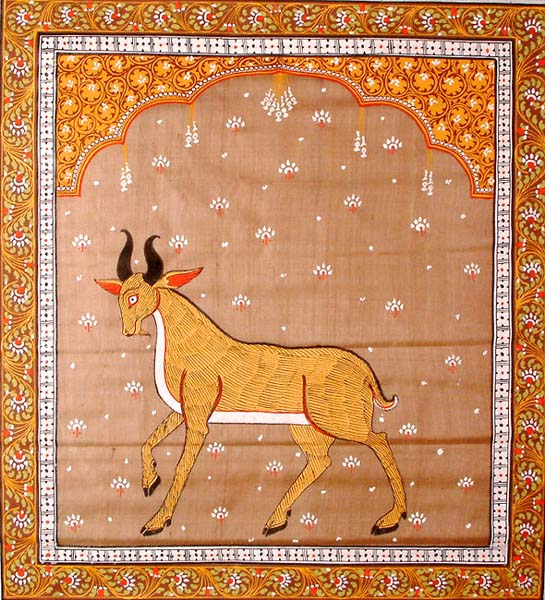
\includegraphics[width=0.5\textwidth]{pics/Aries.png}
 \end{figure}
 

Hindu Drawing of Aries as the Ram
Aries as the Ram is headstrong, assertive, forward movement, determined but obstinate.


 \begin{figure}[H]
 \centering
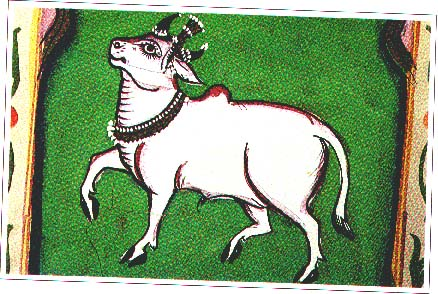
\includegraphics[width=0.5\textwidth]{pics/Taurus.png}
 \end{figure}

Hindu Drawing of Taurus as Bull
Taurus as the bull is strong, steady, creative, earthly and fixed.



 \begin{figure}[H]
 \centering
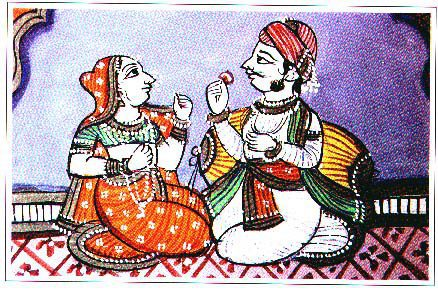
\includegraphics[width=0.5\textwidth]{pics/Gemini.png}
 \end{figure}

Hindu Drawing of Gemini
Vedic astrology regards Gemini as a male and female couple, not as twins as in western astrology.
Gemini is sensitive, volatile, communicative, relationship oriented, ambivalent.

 

\begin{figure}[H]
 \centering
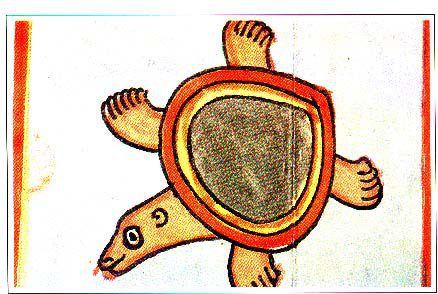
\includegraphics[width=0.5\textwidth]{pics/Cancer.png}
 \end{figure}

 

Hindu Drawing of Cancer as Crab
Cancer as a crab is often hard to understand for the sign of the Moon.
Shows the indrawn nature of lunar emotions but that can also have a power of expression.



 \begin{figure}[H]
 \centering
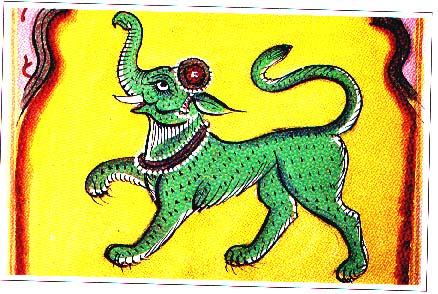
\includegraphics[width=0.5\textwidth]{pics/Leo.png}
 \end{figure}

Hindu Drawing of Leo
Combines Elephant and Lion as sign of Royalty.
Leo is warm, expressive, guiding, leading, but potentially dominating and overpowering.

 
\begin{figure}[H]
 \centering
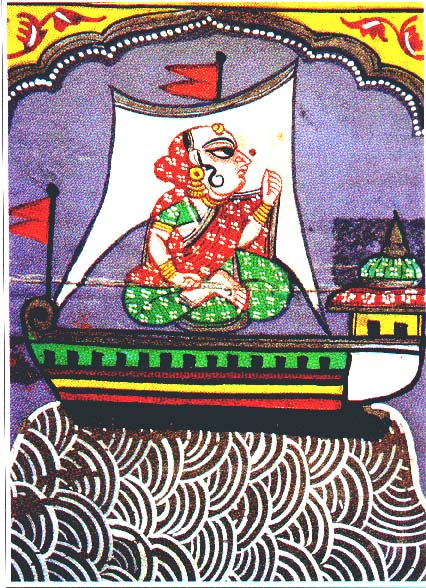
\includegraphics[width=0.5\textwidth]{pics/Virgo.png}
 \end{figure}


 

Hindu Drawing of Virgo
Vedic astrology sees Virgo as a young girl and often a woman overall.
Virgo has both manual and mental skills, is creative, sensitive, vulnerable, yet focused.

 
\begin{figure}[H]
 \centering
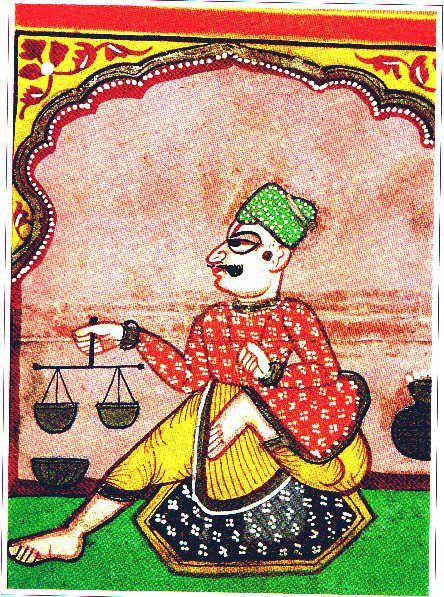
\includegraphics[width=0.5\textwidth]{pics/Libra.png}
 \end{figure}


 

Hindu Drawing of Libra
Merchant Weighing Scales
Libra is concerned with balance, harmony, commerce, communication, both on outer and inner levels.

 

\begin{figure}[H]
 \centering
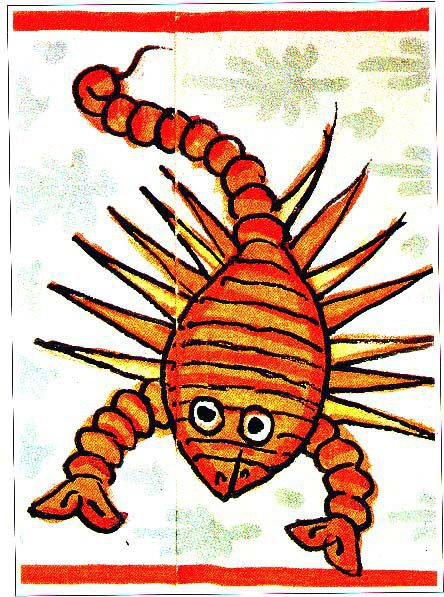
\includegraphics[width=0.5\textwidth]{pics/Scorpio.png}
 \end{figure}

 

Hindu Drawing of Scorpio

Scorpio like the literal serpent has poison in its tail and connects to deep emotional, occult and spiritual energies.


\begin{figure}[H]
 \centering
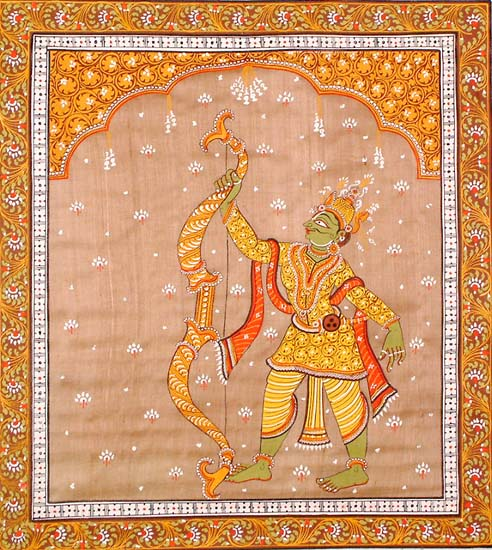
\includegraphics[width=0.5\textwidth]{pics/Sagitarius.png}
 \end{figure}


Hindu Drawing of Sagittarius
As the Bowman
Sagittarius relates to law, dharma, the police, army, gurus, and gives focus.

 

\begin{figure}[H]
 \centering
\includegraphics[width=0.5\textwidth]{pics/Capricorn.png}
 \end{figure}

 

Hindu Drawing of Capricorn
Sometimes a crocodile but other times a mountain goat is used for Capricorn.
Represents the ability to move on Earth and scale its heights but with effort and challenges.

 

\begin{figure}[H]
 \centering
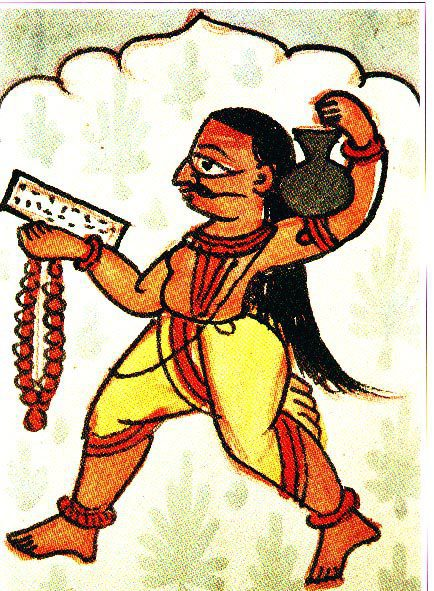
\includegraphics[width=0.5\textwidth]{pics/Aquarius.png}
 \end{figure}

Hindu Drawing of Aquarius
As a man carrying a Water Pot
The water pot is wisdom, the cosmic space, spiritual sensitivity, humanism.

 


\begin{figure}[H]
 \centering
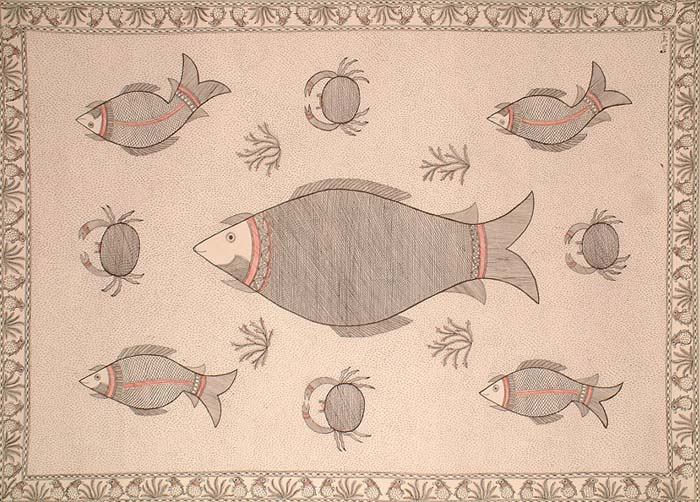
\includegraphics[width=0.5\textwidth]{pics/Pisces.png}
 \end{figure}
 

Hindu Drawing of Pisces as the Fish
The fish indicates absorption, mergence, introversion, intuition and completion.



 

COURSE WORKBOOK FOR EXAMINATION OF SOUTH AND NORTH INDIAN VEDIC CHARTS

The course Workbook, which is supplementary to the other three course volumes, is also referred to in these lessons, as we have already noted. It comes after the other three course volumes in the course index. Just scroll down to find it.

For this particular lesson, once you have completed the lesson material, please examine the first lesson of the Workbook, particularly if you do not know how to read North and South Indian charts and their differences, which the Workbook provides examples for. It teaches you how to read both types of charts. 
\newpage

\section{FOUNDATIONS OF VEDIC ASTROLOGY 2 
Houses, Nakshatras and Planetary Aspects}

In this lesson we continue with basic factors of Vedic Astrology. We summarize the main points in the lesson but have supplementary reading as well. This lesson’s prime topics will be Houses, Planetary Aspects and Nakshatras, but we will begin with additional factors of Planet and Sign Relationship.

 

Numbering of topics continues from the previous lesson (page numbers continue from the book Astrology of the Seers). Again we are introducing these topics, which will be explored in more detail as the course proceeds. Make sure here to get  basic familiarity with the terms and concepts involved. You might want to start with your own birthchart in this examination of chart factors.

 Again in this lesson there will be no lesson tests, study exercises or assignments as the lesson itself requires a lot of examination.

 

\subsection{FURTHER INDICATIONS OF THE PLANETS RELATIVE TO THE SIGNS
SIGNS OF EXALTATION AND DEBILITY }(Astrology of the Seers 103-104)

 

Planets do best when located in their signs of exaltation and suffer in their signs of debility. This is a very important consideration and the basis of certain calculations of planetary strength and weakness. Debility positions are opposite exaltation.

 

\begin{enumerate}
\item[*] Sun is exalted in Aries and debilitated in Libra, exact point 10 degrees.
\item[*] Moon is exalted in Taurus and debilitated in Scorpio, exact point 3 degrees.
\item[*] Mars is exalted in Capricorn and debilitated in Cancer, exact point 28 degrees.
\item[*] Mercury is exalted in Virgo and debilitated in Pisces, exact point 15 degrees.
\item[*] Jupiter is exalted in Cancer and debilitated in Capricorn, exact point 5 degrees.
\item[*] Venus is exalted in Pisces and debilitated in Virgo, exact point 27 degrees.
\item[*] Saturn is exalted in Libra and debilitated in Aries, exact point 20 degrees.
\item[*] Rahu and Ketu are not always given signs of exaltation and debility.
 \end{enumerate}

\subsubsection{Mulatrikona Signs for Planets}

 

Vedic astrology has the special concept of Mulatrikona or root trine, indicating other special places in which planets are powerful. These are mainly in the odd-numbered or positive sign that they rule. Mercury is exceptional in that Virgo is a sign that it rules, that it is exalted in, and that it has its Mulatrikona in. These locations give special power to the planet but not as much as exaltation.

 

\begin{enumerate}
\item[*] Sun – Leo, 4-20 degrees
\item[*] Moon – Taurus, 4-20 degrees
\item[*] Mars – Aries, 00-12 degrees
\item[*] Mercury – Virgo, 16-20 degrees
\item[*] Jupiter – Sagittarius, 00-10 degrees
\item[*] Venus – Libra 0-15 degrees
\item[*] Saturn – Aquarius, 00-20 degrees
  \end{enumerate}

Memorize the points of exaltation and debility and Mulatrikona positions for each planet, both in terms of signs and degrees. This is very important as planets gain strength towards their point of exaltation and lose it towards their point of debility. There are rules of cancellation of debility as well that we will examine later in the course.

 

\subsection{PLANETARY FRIENDSHIP AND ENMITY }(Astrology of the Seers 104-106)
 

Learn to determine planetary friendship and enmity along both natural status (unchanging) and temporal status (changing according to house location in a chart). Note that while Vedic Software will determine this for you, such basic information should be something you can calculate yourself.

 

\subsubsection{Natural Planetary Friendship and Enmity}

 

Be familiar with the two main natural groups of natural friends and enemies.

Sun, Mars, Moon, and Jupiter versus \\
Mercury, Venus and Saturn
 

Planets in the same camp will be natural friends, like Sun, Mars, Jupiter and Moon for one camp, or Mercury, Venus and Saturn for the other. Planets in different camps will be natural enemies, like Sun and Mercury, or Mars and Venus. This is a very important factor.

 

\subsubsection{Temporal or Temporary Planetary Friendship and Enmity}

 

The rule for temporal friends and enemies is also simple, but does require special calculation from the actual birth chart. It reflects the house positions of the individual chart, and is not an overall planetary rule like natural friendship and enmity. These house positions will be explained in greater detail below.

 

Planets located in houses 2,3, 4 or 10, 11, 12, from a given planet’s location will be temporal friends.\\
Planets located in the same house as a given planet or in houses 5-9 from it become temporal enemies.
 

Both natural and temporal friendship and enmity can be combined for a composite indication. Note that most Vedic software will make this calculation for you. Planets do better if located in friendly signs and suffer if located in unfriendly signs. This is something you should always examine in every chart at an initial phase of interpretation. We will examine this factor in detail later in this section of the course.

 

\subsection{3. THE TWELVE HOUSES} (Astrology of the Seers, Chapter 7, the Houses: Domains of Planetary Action, pages 111-144)


The houses (bhavas) are perhaps the most important factor in Vedic astrology and must be clearly understood in qualities. The signs reflect more the individual nature or character, while the houses reflect more our outer manifestation and external life affairs. Become capable of explaining the fields of life that relate to each house.

Lesson 6 will go into great detail on the houses and house rulership issues, which is a topic in ints own right. Note the basics here.

 

The signs and houses correlate in meaning at a general level, with each numbered sign and house having similar indications, (though this should not be taken too far as there are differences between sign and house meanings as well):

 

Aries and first house, Taurus and second house, Gemini and third house,
Cancer and fourth house, Leo and fifth house, Virgo and sixth house.
Libra and seventh house, Scorpio and eighth house, Sagittarius and ninth house.
Capricorn and tenth house, Aquarius and eleventh house, Pisces and twelfth house.
 

For example, the first house will reflect the fiery and assertive qualities of Aries, the second house will reflect the earthy and possessive aspects of Venus, the third house will address communication and expression issues like Gemini, the fourth house will cover mind and emotions like Cancer, the fifth house will cover creative intelligence like Leo, the sixth house will deal with health and disease like Virgo, the seventh house will deal with relationship like Libra, the eighth house will deal with secret and occult issues like Scorpio, the ninth house will deal with dharma like Sagittarius, the tenth house will indicate public work and impact like Capricorn, the eleventh house will address social issues like Aquarius, and the twelfth house will address spiritual issues like Pisces.

 

When the same number house and sign are influenced, the result will be stronger. For example, if a malefic planet like Mars afflicts the ninth sign Sagittarius and the ninth house, there is a greater danger of injury to the hips represented by these factors. If a benefic like Jupiter aspects the fifth sign Leo and the fifth house, it will indicate better past life karma. This is a common principle fo chart interpretation.

 

Western and Vedic astrology usually look at the houses with the same general interpretations, like the seventh house and relationship, but there are some variations. For example, the third house in Vedic is more a martial house indicated by Mars, whereas in western is more Mercurial, lie the third sign Gemini. The ascendent or first house is not a martial house like the first sign Aries but relates more to the Sun as the life energy of the person. These factors will also be examined more later in the course.

 

\subsubsection{Calculation of Houses}
 

There are different ways of calculating the houses (bhava), which can be by sign (rashi), by equal house system or by midheaven systems (Astrology of the Seers 113-115). Houses can be determined:

 

\begin{enumerate}
\item[] 1) By sign, or Equal Sign System – each sign starting with the Ascendant will refer to one house, regardless of the degree of the Ascendant or the planets within it.

\item[] 2) By 30 degree sections starting with the Ascendant or Equal House System. So if for example 10 degrees of Taurus is rising, the region 15 degrees around it will mark the first house, or from 25 Aries to 25 Taurus, with the other houses following in order, the second house as 25 Taurus to 25 Gemini and so on.

\item[] 3) By dividing up the area between the Ascendant and the Midheaven, or Midheaven systems like Sripati or Placidus. Midheaven is a special point that varies by the latitude of the place of birth. The Midheaven is not always 90 degrees from the Ascendant. So if we use the Midheaven as the cusp of the tenth house, we will need to divide up the difference into the houses in an unequal matter. This can be done automatically by current software programs by selecting such house system options.
\end{enumerate}
 

As a special note, Western and Vedic astrology interpret house cusps differently, Vedic astrology makes the cusp the middle of the house , while Western astrology makes it the the beginning of the house, though both regarding the cusp as the most powerful part of the house.

 

\subsubsection{Houses from the Moon}

 

Vedic astrology examines houses from the Moon as well as from the Ascendant. The Moon is a second ascendant or an ascendant in its own right. Houses from the Moon show more how the planets affect our feelings and personal happiness, extending to our social image, while positions relative to the Ascendant relate more to outer factors in the material world and how we are placed relative to the public. Generally we weigh the Ascendant as 2/3 in value and the Moon as Ascendant as 1/3 in value. But sometimes the weight of planetary placements and aspects will favor the Moon.

 

This means that if the same house from the Moon and the Ascendant is affected, the results will be stronger for the issues involved. For example, if the fifth house, which governs children, is afflicted from both the Ascendant and the Moon, say by aspects of Saturn and Mars, difficulties with children is more likely.

 

\subsubsection{Referred Houses}

 

We can turn any house into the Ascendant for that person or factor indicated by the specific house examined, what are called “referred houses” (bhavat-bhavm). For example, we can turn the seventh house the Ascendant and use it for reading the condition of the marriage partner from there. In Vedic astrology the house dial is a like a revolving wheel and can be placed in different parts of the chart relative to different considerations. The normal Ascendant or Rashi chart is the main dial but other secondary factors can also be read. We will examine this factor in greater detail in the Workbook.

 

\subsection{HOUSE QUALITIES} (Astrology of the Seers, pages 117-120)

 

There are three basic qualities of the houses, which are of great importance.\\
Angular or Kendra (1, 4, 7, 10)\\
Succedent  (2, 5, 8, 11)\\
Cadent (3, 6, 9, 12) 
 

Planets are usually stronger placed when kendra or angular positions (Houses 1,4, 7, 10). They are weak when placed in cadent houses (Houses 3, 6, 9, 12) They are of moderate strength when placed in  succedent houses (Houses 2,5,8, 11) These qualities roughly parallel the three qualities of the signs as cardinal, fixed and mutable (moveable, fixed and dual). It is a key consideration in looking at the chart for planetary strengths and weakness.

 

\subsubsection{Additional House Groupings}

Trine (trikona) house locations (1, 5, 9) are also auspicious and powerful, for all aspects of the life and character of a person.\\
Upachaya or increasing house locations (3, 6, 10, 11), as special distinction of Vedic astrology  are good for malefics and give powers of competition, endurance and resistance, gaining more power with age.\\
Apachaya or decreasing house locations (1, 2, 4, 7, 8) houses bring initial benefits but cause planets to lose their strength and value over time.\\
Bad or difficult house locations (6, 8, 12), Duhsthanas are the worst positions in the chart, particularly house 8. All planets weak are if located in these positions, particularly benefics.\\
The houses like the signs (following house-sign correspondence principles) also divided according to to the four elements of Earth 2,6,10), Water (4,8,12), Fire (1,5,9) and Air (3,7,11). For example, the first house like the first sign Aries has a fiery quality.\\
The houses area divided according to the four aims of life as dharma or vocation (houses 1,5,9), artha or prosperity (houses 2,6,10), kama or happiness (houses 3,7,11) and moksha or liberation (houses 4,8, 12).
 

Examine the Description of the Houses in the Astrology of the Seers  (121-128). Learn how to describe each house. Become intimate with its qualities, connections and associations. The houses are the key to chart interpretation. You should know the house qualities as clearly as you know those of the signs.

 

\subsubsection{The natural significators of each house:}

These are special planetary significators unique to Vedic astrology. Some houses have more than one depending upon the factors involved.
Sun and the first house\\
Jupiter and the second house\\
Mars and the third house\\
Moon and the fourth house\\
Jupiter and the fifth house\\
Saturn and Rahu and the sixth  house\\
Jupiter and Venus and the seventh house\\
Saturn and the eighth house\\
Jupiter and Sun and ninth house\\
Sun and Mercury and the tenth house, Mars is also strong there\\
Jupiter and the eleventh house\\
Saturn and Ketu and the twelfth house
 

Jupiter is the significator of several different houses (2, 5, 7, 9, 11). Saturn signifies several houses (6, 8, 12) or all the difficult houses or duhsthanas. Remember that if the natural significator of a house is weak, the house is also likely to be weak.

 

\subsection{PRINCIPLES OF HOUSE RULERSHIP} (Astrology of the Seers, pages 131-142)

 

House rulership, meaning the planet that rules a particular house in a given chart, is one of the most important principles of Vedic astrology and the basis of most interpretations and predictions. Many Vedic astrological combinations or yogas are defined by house rulership (like the ruler of the first house located in the sixth house and the ruler of the sixth house located in the first house, which is a combination that causes disease).

 

Examine the principles of house rulership and see how the meaning of planets changes relative to each ascendant according to the houses that they rule (also called the “temporal status” of a planet). But note that this is covered in a special lesson of its own for more detail.***

 

The complication is that the planets, except Sun and Moon, rule over two houses, one which may have good effects and one that may be difficult. The planet will give the results of both houses it rules, though at different times and different ways. For example, in the case of an Aries ascendant, Mars will rule both the first house (Aries) and the eighth house (Scorpio). Mars rulership of the eighth house will bring in some negative energies, while overall the ruler of the first is regarded as a positive planet.

 

When a planet rules both an angle (1, 4, 7, 10) and a trine (1, 5, 9), it  called a Raja Yoga planet . This gives great power, influence and success in life. Some Ascendants have one planet that does this, like Saturn ruling houses 4 and 5, for Libra Ascendant. Yet Raja Yogas can be created by two planets, if one rules and angle and the other rules a trine.

 

Note that planets function according to the nature of the houses that they rule as well as according to their natural qualities. For example, even when a natural malefic like Saturn rules good houses, it can still cause some difficulties, yet as a Yoga Karaka for Libra ruling houses 4 and 5, its overall effects will be quite good. Never forget to look at the houses they are connected to before judging their effects.

\subsubsection{4. THE TWENTY-SEVEN NAKSHATRAS} (Astrology of the Seers 108-109)
 

At this point we are just introducing the 27 Nakshatras by name and position.  Learn the 27 Nakshatras by name and their positions in the zodiac (the 13 degree 20 minute section that each rules). In the long-term try to memorize them. What you need to know at this point is only introductory. The third section of the course will examine the Nakshatras in great detail and several lessons.

THE 27 NAKSHATRAS\\
ASHWINI, 00 00—13 20 Aries:  “The horses head”. It originally represented the head of the sacrificed horse that symbolized the Sun, the year and the beginning of the cycle of time.Deity—the Ashwins, the twin horsemen (like Castor and Pollux of the Greeks).\\
BHARANI, 13 20—26 40 Aries:  “The bearers”. It is symbolized by the female reproductive organ. Deity—Yama, the God of death and immortality.\\
KRITTIKA, 26 40 Aries—10 00 Taurus:  “The razor”, which is also its symbol. It corresponds to the stars of the Pleiades, the small cluster of six stars in Taurus. Deity—Agni, the God of fire.
ROHINI, 10 00—23 20 Taurus:  “The red or ruddy female deer or antelope”, from its prime star, red Aldeberan or Alpha Taurus. Deity—Prajapati, the lord of creation.\\
MRIGASHIRAS, 23 20 Taurus—06 40 Gemini:  “The antelopes head”, or the head of the sacrificed wild animal or creator God. Now it is related to the head of the constellation Orion, but originally consisted of the three stars in his belt. Deity—Soma, the God of immortality.\\
ARDRA, 06 40—20 00 Gemini:  “The moist”, marked by the red star Betelgeuse, Beta Orion. Deity—Rudra (Shiva), the God of the storm and the bowman or hunter.\\
PUNARVASU, 20 00 Gemini—03 20 Cancer:  “Return of the light”, marked by Castor and Pollux, Alpha and Beta Gemini. Deity—Aditi, the Mother of the Gods who is sometimes identified with the earth but mainly represents the sky.\\
PUSHYA, 03 20—16 40 Cancer:  “The nourisher”, Deity—Brihaspati, the teacher of the Gods. Deity of the planet Jupiter.\\
ASHLESHA, 16 40—30 00 Cancer:  “The serpent”, Deity—Sarpa, the Serpent in all forms.\\
MAGHA, 00 00—13 20 Leo:  “the beneficent”, marked by Regulus, Alpha Leo, Deity—the Fathers or Ancestors.\\
PURVA PHALGUNI, 13 20—26 40 Leo:  “The earlier fig tree”, Deity—Bhaga, the Sun of bliss.\\
UTTARA PHALGUNI, 26 40 Leo—10 00 Virgo:   “The later fig tree”, marked mainly by Denebola, Beta Leo, Deity—Aryaman, the Sun as the beloved, the friend or the helper.\\
HASTA, 10 00—23 20 Virgo:  “The hand”, corresponding to the constellation Corvus. Deity—Savitar, the Sun of inspiration (Apollo).\\
CHITRA, 23 20 Virgo—06 40 Libra:  “The brilliant”, marked by the star Spica, Alpha Virgo. Deity—Twashtar, the Divine craftsman and demiurge.\\
SWATI, 06 40—20 00 Libra:  “The sword”, marked by the star Arcturus, Alpha Bootes. Deity—Vayu, the God of Air or the Wind, also Prana or the life-force.\\
VISHAKHA, 20 00 Libra—03 20 Scorpio:  “The two branches”, marked mainly by Alpha Libra. Deity—Indragni, the dual Gods of Fire and Thunder.\\
ANURADHA, 03 20—16 40 Scorpio:  “Subsequent success, following or devotion”, Deity—Mitra, the Divine friend and lord of compassion.\\
JYESHTA, 16 40—30 00 Scorpio:  “The eldest”, marked mainly by Antares, Alpha Scorpio. Deity—Indra, God of lightning and perception.\\
MULA, 00 00—13 20 Sagittarius:  “The root”, marked by the stars in the tail of Scorpio. Deity—Nirriti, the Goddess of disaster and negation.\\
PURVASHADHA, 13 20—26 40 Sagittarius:  “The earlier victory”. Deity—Apas, the Goddess of the Waters or cosmic sea.\\
UTTARASHADHA, 26 40 Sagittarius—10 00 Capricorn:  “The later victory”. Deity—Vishwedevas, the Universal Gods.\\
SHRAVANA, 10 00—23 20 Capricorn:  “The famous or renowned”, marked mainly by the star Altair, Alpha Aquila, Deity—Vishnu, the Pervador\\
DHANISHTA OR SHRAVISHTA, 23 20 Capricorn—06 40 Aquarius:  “The most wealthy or most famous”, Deity—the Vasus, the Gods of light.\\
SHATABHISHAK, 06 40—20 00 Aquarius:  “What has a hundred medicines”. Deity—Varuna, the God of the cosmic ocean or heavenly waters.\\
PURVA BHADRA, 20 00 Aquarius—03 20 Pisces:  “The earlier auspicious one”, marked mainly by Alpha Pegasus. Deity—Aja Ekapat, the one-horned goat or unicorn.\\
UTTARA BHADRA, 03 20—16 40 Pisces:  “The later auspicious one”, Deity—Ahir Budhnya, the Dragon of the depths.\\
REVATI, 16 40—30 00 Pisces:  “The rich or splendorous”, Deity—Pushan, the Sun in his protective, nourishing or fostering role, particularly relative to the Earth.\\
 

Nakshatras are a subtler division than the signs and help us understand how different parts of signs work. The main practical usage of Nakshtras is for determining planetary periods (dashas) through the Vimshottari dasha system. Yet we do consider Nakshatras as personality types, much like the Sun signs of western astrology. In addition we can judge the effects of planets relative to the Nakshatras in which they are located. Sometimes the Nakshatras are called Lunar Mansions or Lunar Asterisms reflecting their connection with the Moon, but they do have other connections as well and we do not like to use these terms.

 

 



 

\subsection{5. PLANETARY ASPECTS AND ASSOCIATIONS} (Astrology of the Seers, Chapter 9, pages 145-160)
 

Aspects are key factors in astrological interpretation and are highly emphasized in western astrology, where they are calculated with much precision. Planetary aspects or drishtis (meaning views or sights) are also important in Vedic astrology but calculated different than in western astrology, and in a more general manner. The Vedic view of aspects are largely sign based, from that of Western Astrology is degree based. Remember these differences between Western and Vedic usage and determination of planetary aspects. In addition Vedic astrology has other tools like friendship and enmity to judge planetary relations even when specific aspects may not exist. It is not as aspect centered as is western astrology.

 

Learn the major aspects of the planets as they occur by sign.

 

Each planet aspects the sign seventh from it.
For Sun, Moon, Mercury and Venus, these are the only aspects that the planets have.
For example, if the Moon is in Taurus it will aspect Scorpio as the seventh sign from it.
Each planet is also considered to have a direct relationship like an aspect with planets that it shares the same sign, which is called a conjunction.
 

\subsubsection{SPECIAL ASPECTS OF MARS, JUPITER AND SATURN}

 

Mars has additional special aspects on the fourth and eighth signs from its location.
Jupiter has additional special aspects on the fifth and ninth signs from its location.
Saturn has additional special aspects on the third and tenth signs from its location.
 

These special aspects give special power to these three planets, which relate to fire and Pitta (Mars), water and Kapha (Jupiter) and air and Vata (Saturn).

 

\subsubsection{Rahu and Ketu}

Sometimes Rahu and Ketu are given trinal aspects like Jupiter, but this is a secondary opinion. The Rahu-Ketu axis in the chart, including the opposite signs in which it occurs, has its importance in astrological interpretation as well. It forms important Yogas like Kala Sarpa.

 

\subsubsection{Aspects in Divisional Charts}

Note that the same aspects can be used in divisional charts like the Navamsha, though some Vedic astrologers do not use them. We find them to be very useful and always examine them.

 

\subsubsection{Determination of Aspects by Sight}

You should be able to determine these major aspects in the Vedic chart by sight alone, by merely looking at the chart (this is the basis of memorizing charts). That is why there is often  no table of aspects given on the Vedic chart as there is in most western charts. Such simple by sign aspects are easier to see than the degree aspects of western astrology. Yet we should note that when aspects are close by degrees, particularly conjunction and opposition (same sign or opposite sign), they may be stronger in their effects.

 

\subsubsection{Sambandha or Full Relationship between Planets}

Note the principles for determining Sambandha, or complete association between planets, which consists of either conjunction (same sign), mutual full aspect, or exchange of signs like Mars in Gemini ruled by Mercury and Mercury in Scorpio ruled by Mars.. This brings planets into a very close relationship.

 

\subsubsection{Combust Planets}

Planets become combust (burned up by being too close to the Sun). Generally any planet in the same sign with the Sun may likely be combust, generally within fifteen degrees of the Sun.  Generally combust for planets close to the Sun as Mercury and Venus, is not as severe, as they are always not far from the Sun. Of these two combust Venus is the worst. Meanwhile, combust for the outer planets Mars, Jupiter and Saturn is more severe. Combust Saturn is usually the most difficult.

Combustion also affects house ruler. For example, a combust Ascendant Lord can have problems for a person, particularly in terms of health. A combust fourth lord may not bode well for the mother, by way of another example.

 

\subsubsection{Planetary War}

Planetary war (graha yuddha) is generally said to occur if planets are in a conjunction of less than one degree. Generally the planet with the lower number of degrees and minutes will win the war, but some variant opinions are out there. The planet that loses the war becomes much weaker.

 

\subsubsection{Separative Planets}

The Sun, Saturn, Rahu and the lord of the twelfth house (and sometimes Mars) are considered to be separative planets and negate or remove us from the qualities of the house or planet they influence. On the other hand, Moon, Venus and Jupiter tend to strengthen the positive qualities of the house or planet they influence. These rules are extensions of the natural benefic or malefic statys of planets.

Planets or houses with natural malefic planets on either side suffer, called being “hemmed in between malefics” or Papakartari Yoga.\\
Planets or houses with natural benefic planets on either side do well, called being “hemmed in between benefics” or Shubhakartari Yoga.\\
Always look to the disposition of planets around any given planet, mainly in adjacent signs, which can be as important as aspects. Do not examine the planet in a single sign only. Consider not only aspects but planetary proximity, friendships and enmities.

 

\subsubsection{Weight of Planetary Aspects}

Note the weight of aspects in a chart, particularly relative to natural benefic and malefic planets, including which planets have the most influence on the chart.

See which planets or houses have the most aspects upon them in a given chart. As Mars, Jupiter, and Saturn have special aspects they become particularly powerful and generally indicate the fire (Pitta), water (Kapha) and air (Vata) factors in the chart.

 

\subsection{PLANETARY YOGAS}
 

Yogas are general names for combined planetary influences. They are defined in various ways relative to house or sign location, house or sign rulership, and aspects, or even special patterns of planetary influence. The concept of yogas is broader and diverse and can be more important than aspects in Vedic astrology but may include them. Yoga are the culminating and most important aspect of chart interpretation and are the subject of extensive analysis in advanced studies in Vedic astrology. Their are entire books on this subject.

 

Very important and a good place to start are Mahapurusha Yogas, formed by planets being located in an angle from the Ascendant or Moon as well as in their own sign or exalted, does not include Sun or Moon. These are important for determining planetary types of people which are often created by these planetary Yogas.

 

Yogas affecting the Moon are important as the Moon is like another Ascendant. The Moon does best with other planets, particularly benefics, with or around it. It suffers from isolation, which can lead to debility and depression. Yet many other Yogas exist. We will discuss these in greater detail later in the course as they are very important overall.
\newpage

\subsection{6. DIVISIONAL OR HARMONIC CHARTS} (Astrology of the Seers, Chapter 10, Pages 161-172)
 

Normally western astrology only divides the zodiac into twelve parts based upon the twelve signs of the zodiac. In addition, Vedic astrology divides the zodiac into twenty-seven parts based upon the twenty seven lunar Nakshatras.

Yet there are also numerous different divisional (amsha) charts in Vedic astrology, calculated by how we can further divide up the signs. Each divisional chart, also called harmonic chart, has its specific meaning and application. There is the saptavarga or the division of seven important divisional charts.  There is also the list of sixteen divisional charts used.

Common divisions are twofold (hora), threefold (drekkana), fourfold (chaturtamsha), sevenfold (saptamsha), ninefold (navamsha), tenfold (dashamsha) and twelvefold (dwadashamsha).

 

Note that an accurate birth time is necessary to be certain of positions for divisional charts, particularly for their ascendants, though the positions of other planets will not so likely change. Even for the Navamsha, we may not be able to trust the Navamsha Ascendant, which changes every fifteen minutes or so, unless we are certain of the birth chart time to within a few minutes. 

 

Divisional charts vary in importance for in fine-tuning in chart interpretation. For some examples, the Drekkana or harmonic third is important for brothers and sisters, friends, prana and vitality, much like the third house in the birth chart, and has some general value in examining the chart as a whole, particularly the drekkana of the ascendent. The Dashamsha or tenth harmonic chart chart is used along with and much like the tenth house in the birth chart for determining career and success in life, but does not have broader connections.

The Navamsha or divisional ninth chart is most important divisioal chart for all general indications, for the future, for relationship, and for spiritual or ninth house indications. It has a special connection with the Nakshatras, with each Navamsha sign reflecting one-quarter or pada of the Nakshatra.
If the birth time is approximate or the ascendant is within a degree of the shift between one Navamsha and another, read the Navamsha chart with the Rashi Ascendant sign as its Ascendant. This reflects the old system of chart formation in which the positions of the Navamsha were included in the corner of the Rashi chart signs. In other words, you can benefit from looking at the Navamsha even when the birth time may not be exact.
 

Always look at the Navamsha chart at least along with the basic sign (Rashi) chart for primary chart examination. Some Vedic astrologers use the Drekkana or third divisional chart in the same general manner. The other divisional charts have their specific indications, like the Divisional Second or Hora as wealth, the Divisional Third or Drekkana as brothers and sisters. The Divisional Fourth or Chaturtamsha as home. The Divisonal Seventh or Saptamsha as children, the Divisional Tenth or Dashamsha as career. The Divisional Twelfth or Dwadashamsha as parents and past history. We are just noting these divisional charts here and will examine them in greater detail later in the course.

 

Divisional charts also reflect subtler planetary aspects that are not visible from the basic sign chart. Aspects in divisional charts have their place and should be examined carefully, though not all Vedic astrologers do this. New Vedic astrology software can calculate the degree and minute of the planets within the Navamsha. This is interesting but was not part of traditional Vedic astrology and is more a secondary concern.

 

\subsection{7. PLANETARY PERIODS OR DASHAS AND FACTORS OF ASTROLOGICAL TIMING} (Astrology of the Seers, Chapter 11, Pages 173-182)
 

Vedic astrology has its own special set of planetary periods called dashas that is absent in western astrology. There are many types of these planetary periods based upon the Moon’s location in the birth chart, various signs or other special calculations, including Jaimini Chara Dasha and Yogini Dasha.

 

Yet most important of the dashas is the Vimshottari (120 year cycle) dasha system. It is based upon the Nakshatra where the Moon is located in the birth chart, and the planetary ruler of that Nakshatra. In this system, each planet rules over a certain number of years in the 120 year cycle from the Sun (six years), Moon (ten years), Mars (seven years), Rahu (eighteen years), Jupiter (sixteen years), Saturn (nineteen years), Mercury (seventeen years), Ketu (seven years), Venus (twenty years). This cycle works very well, though the specific rationale behind it is not clearly known.

 

In fact, the key to the success of Vedic astrology in timing and prediction rests largely on the incredible accuracy of Vimshottari dasha. Dashas are very important in all chart readings as they reflect the current concerns of the client, which are usually the main reasons they are seeking a consultation. Without relevance to the Dashas other indications in the chart may not be able to manifest.

 

Major planetary periods (Mahadashas)are further divided into minor planetary periods (Bhuktis, Antardashas) based upon the same ratio of the periods ruled by each planet. Vedic astrology software makes these calculations easy and automatic. Minor planetary periods can similarly be broken down into further shorter tertiary periods, though theese depend upon a very accurate birth time, to be certain of their timing. Generally we seldom go beyond the minor period or bhukti, and beyond that point look more to transits.

 

The calculation of different Ayanamshas can change the calculation of planetary periods by some months. Note the Ayanamsha used if you find such variations in different charts. Some Vedic astrologers calculate Dashas by 360 day years instead of the normal years. This also brings in some slight variations.

 

There are certain principles for determining favorable planetary periods that we will discuss later in the course. House rulership of a given planet in the chart is most important in determining whether planetary periods are favorable or unfavorable.

 

Periods of benefic house rulers like the ruler of the ninth house or the fifth house are generally good, for example. Periods of the eighth, sixth or twelfth lords, malefic house rulers, on the other hand, can be difficult. But this is a complex matter requiring examining the chart as a whole, and planets may rule more than one house.

 

The period of the Ascendant Lord is crucial for the overall manifestation of the chart. A strong Ascendant and Ascendant Lord will bring many good results during its period, particularly for career and purpose. A weak Ascendant and Ascendant Lord can be bring disease or difficulties.

 

\subsubsection{GOCHARA OR TRANSITS}

 

Transits, called Gochara in Sanskrit, are current movements of the planets. These can be examined in their own right, like the difficulties possible at times of malefic Mars/Saturn conjunctions. More importantly, they can be applied against positions given in the birth or natal chart, like Saturn transits to the natal Moon (Sade Sathi) which can be very stressful.

 

Transits are very important at in terms of Muhurta, mundane, collective or political astrology, where their influence is prominent in world affairs, national and yearly charts. This is particularly true of transits of the distant planets, Jupiter and Saturn, and the lunar nodes Rahu and Ketu that are involved in eclipses of the Sun and Moon.

 

Relative  to the individual chart, transits modify what may happen during a given planetary period for a person, altering to some degree the results of the planetary period. While certain result may be indicated during a planetary period or subperiod, a special transit may either trigger it or obstruct it.

 

\subsubsection{PRASHNA}

 

Prashna, horary or question based astrology consists of erecting a chart for the specific moment and place that a question is asked. The Prashna chart is interpreted by rules similar to the birth chart, but in some ways different. It may be used when the birth time is not known or if a very specific question is to be examined. We will study it more in Part III of the course, but Prashna will not be a prime or direct part of this course as it forms a subject in its own right that can be quite complicated.

 

\subsubsection{MUHURTA, ASTROLOGICAL FORECASTING AND MUNDANE ASTROLOGY}

 

Muhurta, astrological forecasting and mundane astrology consists of looking for favorable times to perform various actions. Many Vedic astrologers do a lot of such Muhurta work, examining favorable times for marriage, moves, travel, starting a business, mantra initiation and so on.

 

Muhurta is an important and integral part of any Vedic astrology practice. Muhurta is connected to the Panchanga or Vedic soli-lunar calendar, in which the position of the Moon in various Nakshatras is most important, along with its phases (Tithis). Dashas and transits are only secondary.

 

Mundane astrology is related to Muhurta at a collective level and consists of examining charts of countries or their leaders to see the effect of national and world affairs, notably elections. We will examine Muhurta and mundane astrology in detail in Part III of the course, both in terms of Panchanga and Ashtakavarga.

 

\subsection{8. ASTROLOGY AND AYURVEDA, REMEDIAL MEASURES} (Astrology of the Seers, Chapter 12, Pages 183-196)


Ayurvedic Astrology is the more specific theme of this course and is dealt with in detail in the second section of the course, where it is the subject matter of a number of lessons. Here we are only introducing the basics. It is addressed in our book Ayurvedic Astrology that will be referred to later.

For Ayurvedic Astrology, we need to first learn the basic qualities of the three Doshas or biological humors of Vata, Pitta and Kapha and their planetary connections. The doshas are similar to the elements in their qualities and each has a primary elemental connection. Each dosha has planetary connections to various degrees.
Vata (Air) – Saturn, Mercury, Rahu\\
Pitta (Fire) – Sun, Mars, Ketu\\
Kapha (Water) – Moon, Venus, Jupiter\\
Yet planets may reflect more than one dosha, with Jupiter as Kapha and Pitta, Venus as Kapha and Vata, and the Moon varying by dosha as to whether it is waxing and waning and in which sign it is located in

You can supplement your study of Ayurveda by examining various books on the subject. These include the author’s books Ayurvedic Healing, A Comprehensive Guide and The Yoga of Herbs. 

 

The three Doshas also relate to the signs of the zodiac and their respective elements. Earth and Water signs relate more to Kapha dosha. Fire signs relate more to Pitta dosha. Air signs relate more to Vata dosha. But planetary factors relative to the doshas are more important than these sign connections, and various admixtures of influences occur, including relative to the planets exalted in these signs.

Generally the doshic influences of the first six signs from Aries to Virgo are more clear, while those from Libra to Pisces are more mixed as we will discuss in Part III of the course.

Fiery Mars ruled fire-based Aries is Pitta, Venus ruled earth-based Taurus is Kapha, airy Mercury ruled air-based Gemini is Vata, and watery Moon-ruled water sign Cancer is Kapha.
Fiery Sun ruled fire-based Leo is Pitta, airy Mercury ruled earth-based Virgo is Vata, Venus ruled air-based Libra is Vata, fiery Mars ruled water-based Scorpio is Pitta.
Jupiter ruled fire-based Sagittarius is Pitta, Saturn ruled earth-based Capricorn is Vata, Saturn ruled air-based Aquarius is Vata, and Jupiter ruled water-based Pisces is Kapha.
 

The determination of physical constitution can be difficult or complicated from the astrological standpoint as it includes a number of factors, mainly relative to the ascendant that represents the physical body and the sixth house of disease, particularly the dominant planet in the chart or the planetary type. That will be taken up later as well.

 

Certain planets and houses are particularly strong to cause disease, notably malefic planets Saturn, Mars, Rahu and Ketu. The sixth house and sixth sign (Virgo) important in terms of health indications as well as other difficult houses like the eighth and the twelfth. Diseases generally manifest in periods of these disease-causing planets or their transits of significant positions in the chart, or during periods of the ascendant lord if it is weak in the chart.

 

\subsubsection{ASTROLOGY AND PSYCHOLOGY} (Astrology of the Seers, Chapter 13, Pages 189-196)

 

Overall we relate Astrology and Psychology to both Ayurvedic Psychology and Yoga Psychology as well as to Vedantic philosophy, which are interrelated. (Note the authors book Ayurveda and the Mind for understanding Ayurvedic psychology).

The sequence of planets affects  the unfoldment of the karmas of the reincarnating soul of Jivatman. Each planet has psychological implications, as do signs and houses. But this is according to the yogic or Vedic view of psychology, which is very different from that of modern psychology, and extends beyond the physical to the subtle, causal and transcendent realms.

 

By natural status, the Sun is the self, soul or ego, Moon is mind and emotions, Mercury is speech and intellect, Venus is desire, love and affection, Mars is will, motivation and aggression, Jupiter is wisdom, dharma and creativity, Saturn is isolation, withdrawal or negation, Rahu is openness to psychic influences and expansion of collective karma, Ketu is psychic insight, doubt, contraction and withdrawal.

Relative to the houses and their significators, the fourth house  and the Moon is emotional mind, the fifth house and Jupiter is intelligence or buddhi, the first house and Sun is self or ego, and the ninth house and Jupiter is the soul or Jivatman.

 

Vedic astrology is an important psychological tool, which is one of its main and most significant usages. This topic is specially  examined in the Workbook at an advanced level of study, as well as in the lesson on Planetary Types. Here just introduce yourself to the topic.

 

\subsubsection{REMEDIAL MEASURES/ TREATMENT METHODS }(Astrology of the Seers, Chapter 14, Pages 199-233)

 

This topic also relates more to the second part of the course. We will only go through it briefly here. Don’t worry about the details at this point, Vedic astrological is not only predictive and interpretative but provides practical methods called upayas to help us promote positive planetary influence and reduct those that are negative.

 

There are various methods through which weak planets can be strengthened, using colors gems, herbs, aromas, and foods, as well as rituals (flower offerings and fire offerings), mantras and meditation. It can extend to actions of a charitable nature, service, pilgrimage or visiting temples.

The use of gems is central in this regard, with primary gems like ruby for the Sun, pearl for the Moon, red coral for Mars, emerald for Mercury, yellow sapphire for Jupiter, diamond for Venus. blue sapphire for Saturn, hessonite garnet for Rahu and cat’s eye for Ketu .

 

Generally, we use gems to strengthen the Ascendant lord or other benefic planets, like the ruler of the ninth house or the fifth house, when afflicted in the chart. We are hesitant in strengthening natural or temporal malefics through the use of gemstones, like Saturn. We present the rules for determining this in the second section of the course, which can be complicated.

Some people think that a Vedic astrological reading requires a gem recommendation. Actually, yogic and spiritual methods like mantras, yantras and ritual can be more helpful and less expensive than gems, though these do require more effort and time to sustain. While some charts may have weak benefic planets like the ascendent lord that can clearly benefit by a gemstone, other charts have mixed planetary influences for which gemstones for planets may not be of such clear or lasting value.

 

\subsubsection{WORSHIP AND MEDITATION ON THE PLANETS} (Astrology of the Seers, Chapter 15, Pages 227-233)

 

We will only introduce this topic here as it is a main topic of Part II of the course.Yogic and spiritual methods are very important in strengthening the planets and can be better than gems, but require regular practice and devotion to empower.

 

Mantra is most important in this regard, with Vedic astrology having several sets of of name and bija mantras for each planet. Each planet has its ruling deities. It also has its symbols and yantras relate to the planets. This is also covered the book Ayurvedic Astrology and will be detailed later in the course, particularly Part II that has several lessons devoted to this and an outlining of mantras for planets, signs and Nakshatras.

 

\subsubsection{THE ASTROLOGY OF THE SEERS, EXAMPLE CHARTS} (Astrology of the Seers, Chapter 16, 237-268)


This section of the book consists of the examination of charts of various famous people, whose life details and timings are known to us. You should begin examining such charts as you move through the course.progress with the course.  Try to study one chart a week. We will not examine the specific charts in this lesson as they are explained in the book, along with their necessary calculations. Please read that material at your convenience.

Note that we will examine additional instances of chart examination in the Course Workbook that supplements the later lessons of Part I of the course, as well as Lesson 7 on Horoscope Judgement. 

\subsubsection{COURSE WORKBOOOK READINGS}
Make sure to study the Course Workbook 1. Reading North and South Indian Charts, so you know the principles behind reading charts and complete that lesson before looking at any charts!
Make sure you know the mechanics of reading both North and South India charts and how to determine planets, signs, houses, aspects and planetary periods from them.
In addition, begin collecting astrological charts and casting them in the Vedic manner. Start with your own chart and those of your friends and family whose details are known to you. You should get a Vedic astrology software program for this purpose. You can examine the charts of famous or well known people as well. You should continue to look at such charts along with your study of the course overall.

 

First note the mechanics of a chart with the positions of planets, signs and houses, as well as the aspects involved. Note how a person’s planetary periods is reflected in the development of their lives and careers. See if you can determine their dominant planets. See how astrology mirrors their karmas.

 

You can also find books on Vedic astrology that contain charts of famous people, or you can find this information on-line. Or you can get a book of famous charts from western astrology, and transpose them into the Vedic system by subtracting the appropriate Ayanamsha, and then examine the basic or Rashi chart according to major positions. Use your own Vedic astrology computer program to look at and collect birth charts.

 

Learn to look at the daily charts as well, noting the current planetary positions and their relationship to different natal charts or to social and political events in the outer world.  Be aware of the position of the Moon and Sun in the zodiac, as well as outer planets like Mars, Saturn and Jupiter that move more slowly. Note the positions of eclipses and the lunar noes of Rahu and Ketu. Most importantly look at your own birth chart regularly as you learn more about Vedic astrology in the course, and see how Vedic astrology principles are mirrored in your life and character. Try to form a relationship with the planets through their names, mantras and deities.

 

Go out and look at the stars and try to make a connection with them. Note the path of the zodiac, with its twelve signs, and of the Milky Way that dominates the night sky. As an amateur astronomer of many years, I can identify quickly over two hundred deep sky objects with a small telescope that remain a source of great inspiration. Besides planets are wonderful star clusters, nebula, globular clusters and double stars. Remember that the universe dwells within you and the distant stars are part of your own higher mind that can guide. Never forget the role of intuition and meditative insight in astrology.

 

Remember to spend as much time looking at charts as examining the course material or reading books on Vedic astrology. In summary, it is important to read the book Astrology of the Seers, but also remember that much of what is presented in the book will make more sense as you move through the course.

 

\subsubsection{Table of the Planets}
Tabulated from Various Classical Sources (variations do exist!)
Summarizes the main points about the planets

Sun
\begin{center}
\begin{tabular}{ l l l l}
Name	&Surya	&Guna	&Sattva \\
Nature	&Malefic	&Element	&Fire\\
Dosha	&Pitta	&Color	&Red\\
Caste	&Kshatriya	&Sex	&Male\\
Taste	&Pungent	&Tissue	&Bones\\
Abode	&Temple	&Time Period	&Half-year\\
Direction	&East	&Relationship	&Father\\
Psychological	&Ego, Soul	&Physical	&Heart\\
Role	&King	&Deity	&Agni/ Shiva\\
\end{tabular}
\end{center}

Moon
\begin{center}
\begin{tabular}{ l l l l}
Name	&Chandra	&Guna	&Sattva\\
Nature	&Benefic	&Element	&Water\\
Dosha	&Kapha	&Color	&White\\
Caste	&Vaishya	&Sex	&Female\\
Taste	&Salty	&Tissue	&Blood\\
Abode	&Watery Areas	&Time Period	&48 Minutes\\
Direction	&Northwest	&Relationship	&Mother\\
Psychological	&Mind, Emotions	&Physical	&Stomach\\
Role	&Queen	&Deity	&Soma/ Devi\\
 \end{tabular}
\end{center}

Mars
\begin{center}
\begin{tabular}{ l l l l}
Name	&Mangala, Kuja	&Guna	&Tamas\\
Nature	&Malefic	&Element	&Fire\\
Dosha	&Pitta	&Color	&Red\\
Caste	&Kshatriya	&Sex	&Male\\
Taste	&Bitter	&Tissue	Marrow\\
Abode	&Weapons Room	&Time Period	&Day\\
Direction	&South	&Relationship	&Brothers, Siblings\\
Psychological	&Will, Vitality	&Physical	&Small Intestine\\
Role	&Army Chief	&Deity	&Skanda\\
 \end{tabular}
\end{center}

Mercury
\begin{center}
\begin{tabular}{ l l l l}
Name	&Budha	&Guna	&Rajas\\
Nature	&Benefic	&Element	&Earth\\
Dosha	&Vata	&Color	&Green\\
Caste	&Vaishya	&Sex	&Child, neutral\\
Taste	&Mixed	&Tissue	&Skin\\
Abode	&Sports Ground	&Time Period	&Season\\
Direction	&North	&Relationship	&Friends\\
Psychological	&Intellect, Speech	&Physical	Brain\\
Role	&Prince	&Deity	&Vishnu\\
 \end{tabular}
\end{center}

Jupiter
\begin{center}
\begin{tabular}{ l l l l}
Name	&Brihaspati	&Guna	&Sattva\\
Nature	&Benefic	&Element	&Ether\\
Dosha	&Kapha	&Color	&Yellow\\
Caste	&Brahmin	&Sex	&Male\\
Taste	&Sweet	&Tissue	&Fat\\
Abode	&Treasure House	&Time Period	&Month\\
Direction	&Northeast	&Relationship	&Husband, Guru\\
Psychological	&Higher Mind, Conscience	&Physical	&Liver\\
Role	&Minister	&Deity	&Indra\\
 \end{tabular}
\end{center}

Venus
\begin{center}
\begin{tabular}{ l l l l}
Name	&Shukra	&Guna	&Rajas\\
Nature	&Benefic	&Element	&Water\\
Dosha	&Kapha	&Color	&Variegated\\
Caste	&Brahmin	&Sex	&Female\\
Taste	&Sour	&Tissue	&Reproductive\\
Abode	&Bedroom	&Time Period	&Fortnight\\
Direction	&Southeast	&Relationship	&Wife\\
Psychological	&Desire, Love	&Physical	&Sex Organs\\
Role	&Minister	&Deity	&Indrani\\
 \end{tabular}
\end{center}

Saturn
\begin{center}
\begin{tabular}{ l l l l}
Name	&Shani	&Guna	&Tamas\\
Nature	&Malefic	&Element	&Air\\
Dosha	&Vata	&Color	&Blue, Black\\
Caste	&Shudra	&Sex	&Neutral\\
Taste	&Astringent	&Tissue	&Muscles\\
Abode	&Unclean Places	&Time Period	&Year\\
Direction	&West	&Relationship	&Grandfather\\
Psychological	&Suffering, Ego	&Physical	&Colon\\
Role	&Servant	&Deity	&Brahma\\
 \end{tabular}
\end{center}

Rahu
\begin{center}
\begin{tabular}{ l l l l}
Name	&Rahu	&Guna	&Tamas\\
Nature	&Malefic	&Element	&Air\\
Dosha	&Vata	&Color	&Smoky\\
Caste	&Outcaste	&Sex	&Female\\
Taste	&Poisons	&Tissue	\\
Abode	&Wandering	&Time Period	&Eclipses\\
Direction	&Southwest	&Relationship	&Distant Relatives, Foreigners\\
Psychological	&Illusion (Maya)	&Physical	&\\
Role	&Army	&Deity	&Durga\\
 \end{tabular}
\end{center}

Ketu
\begin{center}
\begin{tabular}{ l l l l}
Name	&Ketu	&Guna	&Tamas\\
Nature	&Malefic	&Element	&Fire\\
Dosha	&Pitta	&Color	&Smoky\\
Caste	&Mixed Caste	&Sex	&Male\\
Taste	&Poisons	&Tissue	\\
Abode	&Hiding	&Time Period	&Eclipses\\
Direction	&Southwest	&Relationship	&Ancestors\\
Psychological	&Secret Knowledge	&Physical	&\\
Role	&Army	  &Deity	&Ganesha\\
\end{tabular}
\end{center}
\newpage

\section{PLANETARY TYPES}
 

One of the best ways to understand people is according to their “planetary types.” This is the foundation of all deeper astrological studies and all astrological counseling. It is a key component of Vedic Counseling and helps us with Ayurvedic doshic typologies. Generally, most people are characterized by one planetary type. Individuals will reflect their ruling planet, both in terms of their physiology and psychology. While a certain spectrum of types exists under each planet, as each planet has both higher and lower energies, still each maintains its main characteristics.

 

The following types are indicative only and not to be taken rigidly. Planetary types may sometimes reflect two or three planets in relatively equal strength, so these delineations have to be modified accordingly. Sometimes powerful conjunctions determine the type more than the influence of one planet only.

 

These planetary types are more specific and complex than Ayurvedic types, which they are related to, and which we will examine more in the second part of the course. Sun, Mars and Ketu types are usually Pitta (fire). Moon, Jupiter and Venus are usually Kapha (water). Saturn, Mercury and Rahu are usually Vata (air). But this is not always the case. Planetary types are more psychological than physical in nature. Overall astrological types are much more detailed and reliable than Ayurvedic types, which mainly relate to health. Astrology helps us understand our potentials in all aspects of life.

 

Some people may reflect one planet on an inner or spiritual level but another planet on an outer or mundane level. A person, for example, may have a very devoted, lunar soul but outwardly be very thin and dry or even Saturnian. As usual nature has basic types but plays the full spectrum of her qualities and is not limited by her general laws. Basic planetary types are nine, whereas Ayurvedic types are only three, which provides a much larger scope for variations.

 

 \begin{figure}[H]
 \centering
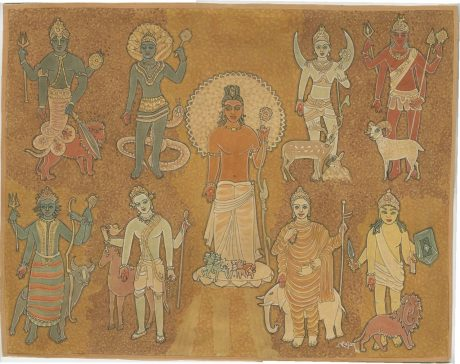
\includegraphics[width=0.5\textwidth]{pics/planetary_types-1.png}
\caption{ The Nine Planets and Their Deities\\
Left to Right Rahu, Ketu, Moon, Mars, first row\\
Saturn, Venus, Jupiter, Mercury, second row\\
Sun Center\\}
 \end{figure}





\subsection{DETERMINATION OF PLANETARY TYPE }
 

There are several ways to determine the dominant planetary type in the chart. The Ascendant or Moon sign best characterizes some people. Others are better represented by a combination of planetary influences so this typology should not be applied rigidly. 

 

The strongest planet in the birthchart usually determines the planetary type. This is usually the lord of the Ascendant, Moon or Sun or the planet that most strongly aspects or influences them. 
Planets in Mahapurusha Yogas often determine the planetary type. The planet nearest the mid-heaven can gain such strength, as does the planet closest to its point of exaltation. The planet that is Atmakaraka in the Jaimini system (possessing the highest longitude or highest number of degrees in any particular sign) often represents the planetary type. The dominant planet usually determines the career, temperament and often the physical type.
One planetary type is not necessarily better than any other is. Higher and lower types exist for each planet. These depend upon the ability of the person to bring in the spiritual energy of the planet. Even spiritually evolved people have their planetary types. An example is the sage Ramana Maharshi who said to be an incarnation of Skanda, the deity of the planet Mars but according to its spiritual energy of knowledge, inquiry and self-discipline.
Planetary types are often evident just by looking at a person. Solar types radiate light and warmth. Lunar types are maternal and receptive. Generally in Vedic Astrology we identify people by their ruling or most powerful planet, not so much by their sign as in Western Astrology.
To teach our clients their planetary types is the key to Vedic astrological counseling and remedial measures. It is the foundation of the astrology of self-knowledge. It does not require a strong predictive ability but even prediction is rendered easier by it. We act according to our ruling planet and the influences upon it. Once we know that planet, a person’s actions are easy to predict.
 



\subsubsection{SUN TYPES}
 

The Sun represents the positive or healthy side of fire energy. Sun types are usually the most healthy of all types because their strong fire energy allows for good digestion, good circulation and the burning up of toxins. They have strong immune systems and seldom come down with serious diseases. Their appetites are strong, even excessive. Their complexion is bright, golden or reddish. Their eyes are golden, perceptive or full of light. Usually they are of moderate build with good muscles. They seldom become overweight or underweight.

 

Their bodies run hot and so they like cool foods and cool climates. Though they prefer much sunshine they are sensitive to direct exposure to the sun. Their main health danger is through overwork or through trying to take responsibility for everything. This can give them heart problems or stomach problems (ulcers).

 

Psychologically, Sun types are characterized by a strong will and a strong vital energy. They are independent and proud, perhaps vain. They like to be leaders or authorities and can gain much power over others. They turn others into their satellites and like to be the bestower of light. They are highly perceptive, a little critical, and can probe deeply into things. They make good scientists or psychologists. They have strong emotions but are seldom overcome by them.

 

Usually Sun types have a philosophical or religious disposition and are ethical in their actions. This comes out later in life, when they often become contemplative. In youth they are largely people of action rather than words and like to command a strong presence in the world. There is something noble or aristocratic about them and they like to associate with people and principles of value.

 

Yet if defeated in life, by disease or by failure to succeed Sun types can fall apart quickly. Their death is often sudden, most commonly by heart attacks. Once their period of success is over and they are no longer in the limelight, they suffer from loneliness and regret. They like to have children but are not usually happy with them. Their standards are too high and their children tend to revolt against them or disappoint them.

 



\subsubsection{MOON TYPES }
 

Moon types are dominated by the water element and show the water element in its greatest flourishing. They have round faces and roundish well‑developed flesh or corpulent bodies. They have attractive faces, hair and features, particularly when young and can be quite beautiful, possessing a certain luminosity. With age they tend to become maternal types and put on weight and water. For women this often happens after the birth of the first child or after the age of thirty. They possess an abundance of vital fluids and have thick, shiny oily hair and skin. Their complexion is usually fair or whitish, and the whites of the eyes are pronounced. Lunar women usually have a good development of the breasts and thighs.

 

Moon types run cold and damp and can easily accumulate phlegm and mucus. They often develop water retention. They have strong lungs and good voices but often suffer from congestion. Usually they live long and are healthy, but may have some constant minor health problems. Often the kidneys are their weakest organ. They are prone to laziness or excessive sleep.

 

Psychologically speaking they are also maternal, loving, caring, nurturing and helpful to others. They are loyal and dependent and make good friends and marriage partners. They are good cooks and are domestically oriented. Their life is centered in home and family. Yet once they overcome their basic shyness and learn to relate on a public level they can succeed socially or politically and become good and sensitive leaders.

 

Moon types are highly emotional, romantic and sentimental and cry easily. Though they are easily hurt, they easily forgive and forget. Their emotional sensitivity is not always a real sensitivity to the emotions of others; sometimes they may be so caught in their own emotional responses that they cannot really see what others are feeling. Yet their emotional sensitivity may give them artistic talents, particularly for the performing arts.

 



\subsubsection{MARS TYPES}
 

Mars represents the negative side of the fire element and its excesses and diseases. While Sun types run hot and dry and maintain a good digestive power, Mars types run hot and wet. They get weakened digestion and easily come down with infectious diseases. They suffer from excess bile and acid. Their blood runs hot and they easily accumulate toxins. They tend towards disease, particularly of an inflammatory nature. They suffer from excess heat and dampness.

 

Generally, however, Mars types possess strong energy and have periods of very good health. But owing to bad living habits, they periodically suffer from acute diseases. They suffer from overuse of alcohol, cigarettes, meat, hot spices, oily and fried foods, overdrinking and overeating. Anger, jealousy and hatred damage their constitution. Usually the liver is their weakest organ and they tend hepatitis, cirrhosis and herpes.

 

Mars types are the most prone to injuries, accidents and traumatic diseases, generally from their own rashness or violent behavior. They often have surgeries or even organs removed. Disease comes to them from outside factors; their basic vitality is usually good. Their health problems are thus not so often necessary as due to their own excessive or blind actions.

 

Physically, Mars types possess moderate build with good muscles. Their complexion tends to be red, with oily skin and they bruise or bleed easily. Their eyes are often red and they tend towards eye diseases. They are sensitive to the sunlight and often wear glasses or sunglasses.

 

Psychologically, Mars types are perceptive, critical and argumentative. They are aggressive and persistent, bold, daring, rash and adventurous. They often get into arguments and conflicts. They make good debaters, speakers, and lawyers. Their sense of logic is strong but often follows their anger more than a real sense of justice. They love to win and hate to lose. Often they will do anything to win.

 

Mars types possess a good sense of mechanics and make good scientists, research workers and are good at working with tools and weapons. They need a practical outlet for their energy to prevent it from going to excess.

 

Mars types, however, are very loyal to their friends and like to form alliances, though usually as opposed to an external threat. They have strong passions and are very possessive. Their sexual energy is strong but not always refined. They tend to overindulge and burn themselves out.

 

A higher Mars type exists as well. This is the highly perceptive and self-disciplined yogi. They are ascetics who mortify their bodies and know how to control their minds. They possess a strong will towards transformation and are willing to pay the price for it.

 



\subsubsection{MERCURY TYPES}
 

Mercury represents the positive side of the air element. Mercury types are very airy, intellectual and nervously sensitive. They are congenial, communicative and compassionate. They are very friendly but tend to be introverted from an excess of thinking. As Mercury is a mutable planet, they often take the physical appearance of the planet strongest to aspect Mercury.

 

Yet Mercury physical types do exist. They are a little tall or short, thin in build, and generally attractive. Their eyes are often greenish and their skin is a little moist, unlike other air types that tend to be dry. They run on the cool side and often have sensitive lungs. They are susceptible to allergies and hay fever as well as to bronchial disorders. Their digestion is often weak or variable. The heart is sensitive and they are prone to palpitations.

 

Mercury types possess good prana or life‑energy, live long, and have a certain glow. They are often athletic and make good runners or basketball players but their endurance is not always high. Often they are athletic when young but shift over to more intellectual pursuits after puberty.

 

Psychologically, Mercury types possess quick minds, a good sense of information and fluent powers of speech. They are good at languages and at statistics but may get their minds caught in trivia. They are witty and have a good sense of humor. They are helpful, service oriented and often take background or dependent roles. They are good at the mass media and make good moderators and interviewers. They may have powers of acting and are good at imitation.

 

Mercury types make good secretaries, teachers and writers. With their strong sense of consideration and their desire to create harmony in life, they also make good doctors and nurses. They love nature, particularly plants, and are good at gardening. They have a refined sense of taste usually free of sensuality. They can develop a deep spirituality once they learn to turn their minds inward.

 



\subsubsection{JUPITER TYPES}
 

Jupiter is the positive side of the water element. Jupiter types possess strong watery constitutions, with good muscles, flesh and fat. All their body tissues are well developed. They tend towards corpulence, mainly later in life, but are seldom much overweight. Their complexion is tinged yellow or golden. They often have great strength and love physical work, exercise and trips into the wilderness. Generally they are very healthy and long-lived. Their most weak organ is their spleen-pancreas. They suffer mainly from overeating sweet, rich and oily foods. Excessive sugar consumption can lead them to diabetes. 

 

Psychologically, Jupiter types are joyful, jovial and content. They tend to overindulgence or self‑complacency. They are friendly, generous and enjoy being with people. They have a strong sense of play and enjoyment, yet seldom become vulgar. They are kind and compassionate and always try to be just. Yet their sentiments and ideals may be too grandiose. They love music, enthusiasm and the display of energy. They are more active and athletic than the other watery types.

 

Generally, Jupiter types are highly moral and ethical people and are devoutly religious. However, they tend towards conventionality in their beliefs and do not like to offend anyone. They have a strong devotion, are the most calm of all types and can easily be at peace within themselves. They develop a contemplative or philosophical bent, as they love to find the larger forces at work in life and join the energy of expansion. Their spirit is positive, expansive and helpful. They seldom worry and tend towards over optimism. They have a natural interest in the spiritual life and in promoting higher causes.

 



\subsubsection{VENUS TYPES}
 

Venus types are often beautiful, being the most attractive of all planetary types. They possess beauty of face, hair and eyes and a general sexual charm and artistic grace. Their tissues are roundish and well developed but they seldom become overweight. Their hands are well formed and delicate, without deep lines. Their sexual vitality is strong and they have somewhat feminine features, even in the men. Yet they have a certain strength and magnetism as well. Venus types are generally healthy, except when they over indulge themselves, in which case they suffer from weakness of the kidneys, reproductive organs, lungs and heart.

 

Psychologically, Venus types are romantically inclined, but not really sentimental. They feel the complementary nature of all forces in life. They have a strong sense of grace. They make good artists and possess a good sense of form and design. They possess good imaginations and have vivid dreams. Their disposition is generally ethical and they possess love and devotion. They are strongly socially minded.

 

Venus types love beauty, comfort and elegance and like to adorn things, including, first of all, their own bodies. They enjoy jewelry and like beautiful homes. They love to display the beauty they possess and to charm others. As such, they can become addicted to luxury but are seldom really greedy. They have a good spiritual potential once they learn the meaning of Divine love. They have good occult or astrological insight through appreciating the beauty of natural law.

 



\subsubsection{SATURN TYPES }
 

Saturn types are usually the least attractive of planetary types. They are unusually tall or short, thin and bony. They may have large noses or large teeth, with unrefined countenances. Their hands and feet tend to be large. Their skin is dry, rough or cracked and tinged brown or black. Their hair is brittle; their nails may be cracked. A more attractive Saturn type does exist, usually as an artist with some Venus influence. The person is dark, elusive, gaunt and striking in appearance.

 

Saturn types are the most disease-prone of all planetary types. They have usually low vitality, poor endurance, and cannot handle much stress. They run cold and have poor digestion and poor circulation. They tend towards constipation and to accumulate waste materials in the body. They are often chronically ill and may pass away prematurely.

 

Psychologically, Saturn types are saturnine. They are overly serious, even morbid. They are usually pessimistic and may suffer from depression. They are generally introverted, solitary and often selfish. The many difficulties that they face in life make them insensitive to the needs of others. They may be miserly and overly calculating. As what they gain only comes through much effort, they are unwilling to share it. They tend toward worry, fear or anxiety, seldom smile and are rarely really happy. They are practically-minded and seldom good dreamers or inventors.

 

Higher Saturn types are yogis, ascetics or monks who renounce the world. They possess detachment and are free of emotional fluctuations. They are beyond the cares of the world. Other Saturn types may be rebels or artists who stand outside of society. Saturn tends to make us unorthodox or non-conformist. Lower types, on the other hand, may be criminals, underworld figures or tyrants (particularly when the influence of Saturn combines with that of Mars). They are suspicious and paranoid, greedy and selfish.

 



\subsubsection{RAHU TYPES}
 

As Rahu and Ketu are not really planets, one may think that planetary types for them do not exist. Yet they can be delineated at least as secondary types. They do have powerful influences on our mind and character, which affects the physical body as well.

 

Rahu types are often born near an eclipse of the Sun or Moon or at the time of the new Moon. They are dark in features and mobile, moody and changeable in temperament. There is a kind of cloud around them, a dark shadow and they have deep-seated psychological problems from the past haunting them. They are a little ghostly in their manners and appearance.

 

Rahu types possess very sensitive nervous systems and often suffer from insomnia or nightmares. On a psychic level, they are partly possessed by something, another entity, curses or unfulfilled longings from past lives. While they easily gain psychic, occult and astral sensitivities, it can be dangerous for them. They may become mediums or do channeling but are easily caught by illusion. Their mental control is tenuous at best.

 

Rahu type women are very clinging but at the same time very willful and like to control their men through crying, hysteria or even threats of suicide. They exert a strange fascination over men that proves destructive. They are tempting, strangely fascinating and alluring.

 

Rahu individuals possess grandiose desires or insatiable cravings, but are incapable of accomplishing ordinary things. When they have success in the world, it is unfulfilling and may cause mental breakdowns or other psychological problems. Their egos are inflated but weak. They are either dominating or dominated. They suffer from a certain vanity and have unrealistic fantasies. Spirituality comes to them only after a great deal of self-examination and learning of self-control.

 



\subsubsection{KETU TYPES}
 

Ketu types are introverted and individualistic to the point of eccentricity. They go their own way and rebel against the social order. Often they debase themselves by following lower social influences. They possess self‑doubt and even while they go their own way, they are confused about what it really is. They are very sensitive to criticism and react in a strongly defensive manner. They often suffer from neuromuscular disorders and have a lack of coordination. They are prone to accidents, surgery, or violence and suffer in wars and other mass catastrophes.

 

Ketu types are perceptive but their focus is narrow. Their minds are critical, negative and highly discriminating. They tend to be overly serious and are seldom really happy. They are often fixated on the past and may make good historians or archaeologists. They are probing, searching and examining. Once a problem enters their minds they will go over it endlessly until they find an answer. Often they are so doubting that they never arrive at an answer or if one comes, they do not trust it. They are best at obscure research and are able to find the light in darkness, though they may miss the light of day.

 

Higher Ketu‑types are yogis (Jnanis) and possess much spiritual knowledge and insight. They see the illusory and transient nature of the world and go their own way regardless of circumstances. They are free of karma and desire. They are able to see through and go beyond the ego. They are a law unto themselves. They may not be recognized or appreciated but they are beyond the praise or blame of the world.

 

 

\subsection{SUMMARY OF PLANETARY TYPES}
 

We can ascertain all the variations in human types in planetary terms. We can understand all human problems according to the energetics of the planets. We can determine all psychological problems according to the functioning of the planets on a lower level, and spiritual growth as their function on a higher level. Yet for this we have to look deeply at the planets and not just according to stereotypes.

 

The key to inner growth is to move from the lower to the higher functioning of our planets. This is to become conscious of their workings and their potentials on both inner and outer levels. It also requires an integration of the planetary influences within us.

 

\subsubsection{DUAL PLANETARY TYPES}

 

For people who have two planets of equal strength, a mixed type will emerge. For example, a Sun-Moon type will have a strong personality, both in its active and receptive, solar and lunar sides. A Mars-Jupiter type will give a Jupiterian expansiveness to the Mars work and action principles. A Mercury-Jupiter type will have an expansive but detailed and strong intelligence. A Mars-Venus type will have a strong sexuality, passion and vital will.

 

Sometimes higher and lower planetary influences combine as well. For example, a person may have a higher Jupiter influence with a lower Mars energy. They may have much expansiveness, faith and a philosophical disposition but allied with a lower Martial will to impose it upon others.

 

\subsubsection{SECONDARY TYPES}

 

Secondary planetary types also exist. A person may be primarily Moon but Venus secondarily, for example. They will have a strong lunar, maternal or receptive feeling nature, yet with a significant need for affection and beauty, Venus traits. Another person may be primarily Moon but secondarily Mercury. They will be intellectual, poetic and socially minded.

 

Thus, we can understand the differences between people of the same planetary type by what planet is second in their nature. This affords us much more specificity in our interpretations.

 

\subsubsection{WEAK PLANETARY TYPES}

 

Sometimes a weak planet characterizes a person – they can be seen by the planetary strengths lacking in their nature. For example, if the Moon is weak in a chart, fear, moodiness and an inability to relate to people will characterize the person. Such an influence may be so strong that it is best to aim at correcting this weak planet rather than dealing with the planetary type.

 

Most often, however, weakness of a planet is caused by another planet being too strong or pronounced. For example, a strong or prominent Saturn and Rahu and their malefic influence are usually behind a weak Moon. Hence, Saturn or Rahu types usually have weak Moons.

 

\subsubsection{INDEX OF PLANETARY INFLUENCES }

 

While the basic planetary type is crucial, we must remember that each of us contains the influences of all the planets. Through Vedic Astrology, we can examine the relative strength and weakness of all the planets. This includes two main factors:

 

The first and most significant factor is the general strength of the planet by house, sign and aspect.
The second is the friendship and enmity between planets, particularly that between the planet and the ruler of the sign in which it is located (its dispositor).
 

Whenever we examine a chart for a person we should help them understand not only their planetary type but the general meaning of all the planets and their relative strength or weakness of their chart overall. In the end, each chart, like a painting, will have its own design and special way to understand it. Houses, signs and planetary periods also strongly color our lives. Yet one planet will usually stand out, either as the planetary type or the dominant planetary influence for a giving time or given concern.
\newpage

\section{THE TWELVE HOUSES AND HOUSE RULERSHIP, ADVANCED STUDY}
 

The houses are prediction wise more important than the signs in Vedic Astrology. Most planetary combinations (yogas) are defined in terms of the houses – like the ruler of the second house of livelihood located in the twelfth house of loss being a yoga for poverty. Vedic Astrology regards planets more as house lords than it does as sign rulers. Hence, to proceed with a deeper study of Vedic Astrology, we must examine this issue of house rulership specifically. We should remember the houses that a planet rules from the Ascendant and the Moon. We should look at it first as a house lord and only secondly according to its natural status.

 

While we have already recommended the background of the Houses, much detail will be added here. The house lords will carry the energies of the houses that they rule and influence their condition, their gains and losses as well.

 

For additional information on the houses relative to Raja Yoga, please examine Lesson 4 of the Workbook. For the different house rulerships from different Ascendants and how they function, please examine Lesson 3 of the Workbook (This material helps you understand the signs better as well). This material is extremely important and has a number of charts examined along with it.

 

\subsection{MEANING OF THE HOUSES}

\paragraph{FIRST HOUSE}

Foundation of the chart overall, body, health, vitality, success in life, career, identity, ego, soul, self

\paragraph{SECOND HOUSE}

Livelihood, speech, self-expression, face, early childhood, literary abilities

\paragraph{THIRD HOUSE}

Vitality, prana, brothers and sisters, youth, friends, arms, sense organs (cognitive and motor), skills, arts and crafts, hobbies, interests, information

\paragraph{FOURTH HOUSE}

Mind, emotions, psychology, mother, heart, home, house, vehicle, education (particularly at home), faith, devotion

\paragraph{FIFTH HOUSE}

Intelligence, intellect, education, judgment, values, children, creative intelligence, dharma, past life influences

\paragraph{SIXTH HOUSE}

Enemies, diseases, injuries, distant relatives, foreigners,  litigation, work, struggle, competition

\paragraph{SEVENTH HOUSE}

Partnership, marriage, social projection, career, success, happiness

\paragraph{EIGHTH HOUSE}

Death, longevity, subtle influences, the occult, medicine, Tantra, collective resources, corporations,  loss of fame, deception, calamities

\paragraph{NINTH HOUSE}

Dharma, religion, spirituality, the father, grace, good fortune, luck, higher education, principles, values, belief, conscience

\paragraph{TENTH HOUSE}

Career, vocation, karma, public success, public influence, recognition, fame, elevation

\paragraph{ELEVENTH HOUSE}

Gains, income, achievements, titles, rewards, social recognition, social influence, associates, administrative abilities

\paragraph{TWELFTH HOUSE}

Loss, liberation, debility, selflessness, service, retirement, rest, sleep, samadhi



 

\subsection{HOUSE LORDS}
 

We introduced the basic information on house lords and their meaning in the Astrology of the Seers. Here we will go into more detail on this important and complex subject.

 

Generally, planets are auspicious or inauspicious relative to the houses they rule as calculated from each particular ascendant. This is their “temporal” status, regardess of what their natural status may be.
However, planets are generally good for the affairs of the houses that they rule. Even the lord of a bad house, like the eighth, will be good for the affairs of that house like longevity.

\subsection{HOUSE RULERSHIP TABLE}
TEMPORAL DISPOSITION OF PLANETS
 
\begin{center}
\begin{tabular}{ l l l l l l l l}
Sign &Sun	&Moon	&Mars	&Mer.	&Jup.	&Venus	&Saturn \\
Aries	& 5 A	&4 A	&1, 8 A	&3, 6 I	&9, 12 A	&2, 7 I	&10, 11 I\\
Taurus	&4 N	&3 I	&7, 12 I	&2, 5 A	&8, 11 I	&1, 6 A	&9, 10 *\\
Gem.	&3 I	&2 N&	6, 11 I	&1, 4 A	&7, 10 I	&5, 12 A	&8, 9 N\\
Can.	&2 N	&1 A	&5, 10 *	&3, 12 I	&6, 9 A	&4, 11 I	&7, 8 I\\
Leo	&1 A	1&2 N	&4, 9 *	&2, 11 I	&5, 8 A	&3, 10 I	&6, 7 I\\
Virgo	&12 N	&11 I	&3, 8 I	&1, 10 A	&4, 7 I	&2, 9 A	&5, 6 N\\
Libra	&11 I	&10 N	&2, 7 I	&9, 12 A	&3, 6 I	&1, 8 A	&4, 5 *\\
Scor.	&10 A	&9 A	&1, 6 A	&8, 11 I	&2, 5 A	&7, 12 I	&3, 4 I\\
Sag.	&9 A	&8 N	&5, 12 A	&7, 10 I	&1, 4 A	&6, 11 I	&2, 3 I\\
Cap.	&8 I	&7 N	&4, 11 I	&6, 9 A	&3, 12 I	&5, 10 *	&1, 2 A\\
Aqua.	&7 I	&6 I	&3, 10 I	&5, 8 A	&2 ,11 I	&4, 9 *	&1, 12 A\\
Pisces	&6 N	&5 A	&2, 9 A	&4, 7 I	&1, 10 A	&3, 8 I	&11, 12 I\\
 \end{tabular}
\end{center}
 

A = Auspicious, I = Inauspicious, N = Neutral,

* = Very Auspicious, Raja Yoga Karaka

 

This is a general table and requires more specificity. It should not be applied mechanically:



\subsection{\textbf{Note Audio Explanation of Principles of House Rulership Followed by Detailed Examination}}


The ruler of the ASCENDANT is generally good as it aids in the prospering of the chart overall. Yet if it is a natural malefic or rules another house that is malefic in nature, its benefic status is tainted and it may under certain circumstances give bad results. \\
The ruler of the SECOND HOUSE is generally neutral, though good for wealth and livelihood, which it rules. Yet as a maraka or death-causing planet, it has a negative side as well, particularly when the chart is weak.\\
The ruler of the THIRD HOUSE is generally inauspicious, as it is an impulsive, impetuous force, works through power and can cause oppression or opposition. However, it is usually good for brothers, friends and personal assertion, which the house rules.\\
The ruler of the FOURTH HOUSE, as an angle or kendra, is good if a natural malefic but bad if a natural benefic.  If strong, it is good for the mother and for peace of mind and emotional well-being, can promote devotion.\\
The ruler of the FIFTH HOUSE is generally good, as the fifth is a trine and gives good karmic results, bringing wisdom and good karma into the chart, along with children and creativity.\\
The ruler of the SIXTH HOSUE, a house of disease and injury, is generally bad and can cause harm or at least promote enmity or disease.\\
The ruler of the SEVENTH HOUSE, as an angle, follows the same rules as that of the fourth and is good for the partner. As a maraka, it can cause some trouble for the health later in life.\\
The ruler of the EIGHTH HOUSE, a house of obstacles, opposition and negativity, is generally inauspicious, though it does aid in certain careers like medicine, insurance or corporate positions.\\
The ruler of the NINTH HOUSE, as the best trine and house of fortune, is usually good. It gives grace, good karma, good fortune and well-being, and aids in education and spiritual knowledge.\\
The ruler of the TENTH HOUSE follows the same rules as that of any angular ruler and represents the best angular house. When strong the career and overall success of the person will prosper.\\
The ruler of the ELEVENTH HOSUE is good for income or gains, which its house rules. However, it is malefic for the chart as a whole because it has a disruptive, impulsive, anarchic influence and can cause disease and injury like the sixth lord.\\
The ruler of the TWELFTH HOSUE is generally inauspicious but more often neutral in character, depending upon the other house it rules. It can cause loss but can also connect us to foreign groups or ideas.\\
 

When a planet rules two houses, we must combine the natural status of the planet along with the two houses it rules, as well as its relationship with the ruler of the Ascendant.

 

For example, Saturn rules the eighth and ninth houses for Gemini Ascendant, a good house and a bad house. It is naturally malefic but normally a friend of Mercury, which rules Gemini. Its mulatrikona sign Aquarius governs the ninth. Hence, it would be mixed but slightly good for Gemini. However, if it is a temporal enemy of Mercury in the chart, its results would tend to be bad. Depending upon its aspects and associations, it can function either as the lord of the eighth or ninth houses. Planetary positions in each chart will modify these principles of house rulership.

 

When we classify a planet as neutral or mixed for an ascendant, we mean that it can give both good and bad results, though in different areas of life, not that it will give only neutral effects.

 

When Saturn rules the eighth and ninth, for example, it is still tainted by its eighth house rulership and will give some negative effects. Its effects will not simply cancel each other out but be good for some things and bad for others.



\subsection{PLANETS BY ASCENDANT RELATIVE TO HOUSE RULERSHIP}
 

The following defines each planet by ascendant, its particular affects as lords of certain houses. Never look at a planet just as its natural status like Jupiter as the great benefic Jupiter. Always consider its house rulership relative to the particular ascendant. The indications are typical and can be modified or expanded. This is an important reference table.

 

\subsubsection{Aries Ascendant}
 

\paragraph{Sun}

The Sun, as ruler of house 5, is a planet of creative intelligence, progeny, counsel and good karma. It is very auspicious. It makes Aries types good lawyers, advisors or psychologists and gives them strong passions and good creativity. Yet it usually indicates that they will not have many children and can burn their hearts out through too much willfulness, impulsiveness, drama and passion.

 

\paragraph{Moon}

The Moon, as ruler of house 4, is a planet of emotion, home, happiness, and the mother. It is generally auspicious but according to some, suffers somewhat by owning an angle as a benefic. Hence, Aries types can suffer from being too emotional or worrying too much. But the Moon is not usually very harmful for them.

 

\paragraph{Mars}

Mars, as ruler of houses 1 and 8, is a planet of the self and the body. It is generally auspicious but tainted by its rulership of the eighth. It is a double indicator of longevity, ruling two houses of longevity. It shows that Aries people may be prone to vice or lack of ethics on one hand, or may conduct some profound research on the other (these being the positive and negative meanings of the eighth house). It shows a potential for them to be headstrong and impulsive, and potentially self‑destructive. Yet it can give deep insight and profound intelligence (the higher aspects of the eighth house).

 

\paragraph{Mercury}

Mercury, as ruler of houses 3 and 6, is a planet of energy, impulse, friendship, injury, disease, egoism, enmity, and prowess. It shows a potential for conflict with friends. Aries types generally possess an overly critical intellect, through which they can become involved in conflict and controversy. They can also suffer from nervous burnout from too much thinking. Hence, Mercury is generally inauspicious for Aries types.

 

\paragraph{Jupiter}

Jupiter, as ruler of houses 9 and 12, is a spiritual planet giving grace and showing renunciation through wisdom. Aries types have a strong sense of principle and can be moved by a higher idealism and benevolence. On a more general level, it can give luck, fortune and status. It is very auspicious, perhaps the best planet for Aries. Yet its twelfth house rulership can taint its influence, particularly later on in life.

 

\paragraph{Venus}

Venus, as ruler of houses 2 and 7, is a planet of wealth and relationship, often showing gains through marriage and partnership, or multiple partners. For Aries types, partnership may be bound up with work and finances. They need to work with others to balance out their overly individualistic nature. Venus is inauspicious and becomes a maraka or death-dealing planet when the chart is weak or afflicted..

 

\paragraph{Saturn}

Saturn, as ruler of houses 10 and 11, is a planet of power, prestige, gains, impulse, injury, disease and egoism. Aries types have an ambition for success and achievement that tends to become excessive and must be controlled or it will lead to a fall. They can burn themselves out prematurely through overwork if afflicted. Saturn is perhaps the most inauspicious planet for Aries.

 

\paragraph{Overall}

The Sun and Jupiter (rulers of houses 5 and 9) give spiritual power and character. Mercury and Saturn (ruling houses 6 and 11) show excessive impulsiveness and a critical nature. The Sun and Moon together (ruling houses 4 and 5) give a powerful impact on life and a strong creative nature. The Sun and Moon, or the Moon and Jupiter (lords of angles and rines together) give Raja Yoga (great prestige).

 

Aries is the most one‑sided of ascendants and, usually, the easiest to judge. This is because house and sign rulers always correspond. When the first sign marks the first house, all the other signs will mark the other corresponding houses. Hence, planets are double significators for Aries. The Moon, for example, indicates the mother by its nature and by its rulership of the fourth house. Any influence on the Moon will, therefore, doubly affect the mother. For this reason, Aries ascendant can make for a very strong or a very weak chart.

 

As a cardinal and a fire sign, Aries types act with strength and decisiveness, which may be impulsive or excessive. Their planets manifest this angularity. Aries types are good at starting things but may consume themselves like meteors. They have strong minds and much energy in their heads but can be headstrong.

 

\subsubsection{Taurus Ascendant}
 

\paragraph{Sun}

The Sun, as ruler of house 4, is a planet of emotion, home and happiness. It shows the tendency of Taurus types towards expansion through property and comfort, as well as their soul tendency towards grace or beauty. Its shows their tendency to worry and possible separation from their home life in their attempt to expand their sphere of material development. It is generally neutral, considered slightly auspicious by some (by being a malefic ruling an angle), slightly inauspicious by others (by its basic nature).

 

\paragraph{Moon}

The Moon, as ruler of house 3, is a planet of energy, interest, motivation, impulse and enthusiasm. It shows the strong sense of curiosity of Taurus types, which may lead them into artistic pursuits on one hand, or superficial hobbies on the other. It is generally inauspicious and shows the tendency of Taurus to emotional impulse and excess.

 

\paragraph{Mars}

Mars, as ruler of houses 7 and 12, is a planet of relationship, sexuality and passion. It indicates an impulse towards sensuality, which may lead to loss of energy and dissipation. It can also show financial loss or expenditure on relationship. It shows the Taurus capacity to aggression in relationship and their high passion levels. It is inauspicious.

 

\paragraph{Mercury}

Mercury, as ruler of houses 2 and 5, is a planet of speech, education, intelligence and creativity. It shows the inherent artistic and poetic sense of Taurus types – their beauty and formal order of expression. They prosper through good communication. It is generally auspicious.

 

\paragraph{Venus}

Venus, as ruler of houses 1 and 6, shows a tendency to work with foreigners. It shows how Taurus types can create their own diseases or enmity in life by their excessive inertia, obstinacy and clinging to form. It is generally auspicious but Venus is tainted somewhat by its rulership of the sixth.

 

\paragraph{Jupiter}

Jupiter, as ruler of houses 8 and 11, is a planet of willfulness, violence and destruction. It shows a danger towards excessive material expansion and self‑righteousness, and may cause obesity. It is generally inauspicious and causes excess, but its nature somewhat balanced by Jupiters natural benefic qualities.

 

\paragraph{Saturn}

Saturn, as ruler of houses 9 and 10, gives honor, prestige, power, position and great skill. It shows the enduring drive towards practical achievement in the Taurus nature, which often does not become strong until old age. When Saturn is too strong, Taureans can be cold and controlling, neutralizing their otherwise grace. Saturn is very auspicious giving Raja Yoga.

 

\paragraph{Overall}

The Moon, Mars and Jupiter (rulers of houses 3, 8 and 12) bring danger, rash action, and sudden downfalls. Mercury and Jupiter (ruling houses 5 and 11) together make for profound intelligence. Saturn gives Raja Yoga and great accomplishments, particularly if combined with Mercury, which can give them a spiritual nature. Venus and Mars together make for a highly sensual disposition and possible dissipation. For Taurus Venus gives more success if tempered by Saturn.

 

As a fixed and earth sign, Taurus types are slow to initiate things but very good at perfecting form. They are often conservative and once they are into something are slow to let go. Hence, the planets for Taurus manifest slowly but thoroughly.

 

\subsubsection{Gemini Ascendant}
 

\paragraph{Sun}

The Sun, as ruler of house 3, shows Geminis soul of curiosity, intellectual impulse and strong opinions, which can cause them to rely too much on their own thoughts and energies. It also shows their strong sense of friendship and tendency to form alliances, particularly for the working out of their ideas. It is inauspicious.

 

\paragraph{Moon}

The Moon, as ruler of house 2, gives fluency of speech, good education and capacity to gain wealth. It endows Geminis with highly developed minds. Additionally, it indicates their great sensitivity and need for emotional nurturing as children. It is generally neutral.

 

\paragraph{Mars}

Mars, as ruler of houses 6 and 11, is triply (by nature and by ruling two houses of injury) a planet of violence. Geminis tend to suffer from accidents and injuries from their absent‑mindedness or through blindness generated by their own opinionatedness or excessive idealism. They suffer from excessive activity, overexertion or hypersensitivity leading to nervous burnout. Mars is very inauspicious for them.

 

\paragraph{Mercury}

Mercury, as ruler of houses 1 and 4, indicates their close alignment of self and mind. While this gives directed mental powers, it can detract from objectivity in regard to the self. It can cause an overly self‑sensitive psychological nature. Any aspects to Mercury will triply affect the mind because the planet rules the self, the ascendant, the mind, and the fourth house and naturally indicates the intellect as well. Mercury is auspicious as the ascendant lord.

 

\paragraph{Jupiter}

Jupiter, as ruler of houses 7 and 10, shows a strong will and idealism as well as a seeking of power and prestige in relationship. Geminis over express themselves in relationship, which can lead to dissipation and a diffusion of energy. Though generally inauspicious, it is mainly when weak by house, sign or aspect that Jupiter will give bad results.

 

\paragraph{Venus}

Venus, as ruler of houses 5 and 12, is a planet of passion and luxury. It shows the strong artistic sense and wealth-giving power of Gemini but also its excessive sexuality that leads to loss or dissipation. Gemini types suffer from nervous stimulation and can become enervated through sex. On a higher level, Venus gives them creativity and intelligence and general good fortune. It is probably the most auspicious planet for the ascendant.

 

\paragraph{Saturn}

Saturn, as ruler of houses 8 and 9, can function as a spiritual planet, giving profound intelligence. It also shows the basic ambiguity and contradictions of Gemini types, which can destroy them. They get caught in the dualities of their own minds. Hence, Saturn becomes neutral in its function, though perhaps slightly auspicious (with its Mulatrikona sign Aquarius marking the ninth).

 

\paragraph{Overall}

Venus and Mercury (ruling houses 4 and 5) together give Raja Yoga. Venus and Saturn (rulers of houses 5 and 9) give much success inlife.  Mercury and Saturn (ruling houses 1 and 9) give spiritual awareness. Mars with Jupiter or the Sun (rulers of houses 6, 7 and 11) creates a disturbed or hyperactive mind, which may lead to difficulties or disasters.

 

As a mutable and air sign, planets for Gemini tend to scatter and diffuse their energy. Their action is often quick, premature, irregular and hard to predict. Though a good ascendant for the mind, it is not so good for long term success in the world and has a tendency towards disease and injury. In this computer age, Gemini has a new advantage, however, with their quick and abstract minds.

 

\subsubsection{Cancer Ascendent}
 

\paragraph{Sun}

The Sun, as ruler of house 2, is a planet of speech, wealth, and education, giving good earning capacity and ruling powers. Yet it can give great expenditures and material responsibilities, if afflicted. Cancer types put their soul into their communications. The Sun is generally neutral for them.

 

\paragraph{Moon}

The Moon, as ruler of house 1, is the planet of self and basic orientation in life. It shows that for Cancer types their soul and emotions are closely linked. This affords them a great sympathy and sensitivity that may render them passive or influenced by social trends, which they can also become exponents of. Their heart is in human feeling and emotional considerations are very important for them. The Moon is auspicious as the lord of the ascendant.

 

\paragraph{Mars}

Mars, as ruler of houses 5 and 10, gives great power. Cancer types need to marshal their energies and act with force and discipline in order to succeed in life. Mars is very auspicious and gives Raja Yoga. Yet as a natural malefic can still cause harm at times.

 

\paragraph{Mercury}

Mercury, the ruler of houses 3 and 12, shows their tendency towards loss of energy and mental power through too much emotion. They may also suffer losses through friends, as their alliances may be more based upon sentiment than true affinity or business sense. It is generally inauspicious.

 

\paragraph{Jupiter}

Jupiter, as ruler of houses 6 and 9, shows their basic ethical nature and sympathy even towards enemies or foreigners. If weak, it shows losses through them. Excess of emotion over good fortune may cause problems as well. Jupiter is generally auspicious but at times can function negatively as lord of the sixth (particularly when several malefics are in the sixth).

 

\paragraph{Venus}

Venus, as ruler of houses 4 and 11, shows their seeking of property and comfort in the home life. It is their planet of sensuality and shows the sentimentality and attachment they must learn to control. It often gives them gains through property or vehicles. It is generally inauspicious.

 

\paragraph{Saturn}

Saturn, as ruler of houses 7 and 8, shows their tendency to relationships with those of inferior status, who may be hard working or harsh in speech. This may lead them to some kind of disgrace or cause them self-examination. Cancer types tend to suffer in partnership. Their over emotionality may make them manipulative and dominating. Saturn is the most inauspicious planet for them.

 

\paragraph{Overall}

For Cancer ascendant, Mars and Jupiter (rulers of houses 9 and 10) give political and social power and prestige. Mars gives Raja Yoga even by itself. Jupiter and the Sun (ruling houses 2 and 9) give intelligence. Mercury and Venus (ruling houses 3 and 11) give difficulties through too much emotion. Saturn and Venus (ruling 8 and 11) bring difficulties and downfall through excessive materialism.

 

As a cardinal and water sign, Cancer types are able to express their emotions and have an emotional impact on others. Their planets act with gentleness and force combined, seldom in a harsh manner. They often achieve much in life through their ability to relate to others and their diplomatic skills. Their own initial shyness and emotional sensitivity (lunar nature) often slows them down.

 

\subsubsection{Leo Ascendant}
 

\paragraph{Sun}

The Sun, as ruler of house 1, shows the character, will, ego and soul of Leo types. Leos possess a strong passion for life and self‑expression, a good creative intelligence, as well as a certain aristocracy of the spirit that may degenerate into vanity or ostentatiousness. They can develop charisma but may be self‑dramatic or self‑centered. The Sun is doubly a self‑indicator as both lord and indicator of the first house and so aspects on it will be doubly strong for character issues. It is auspicious as the lord of the ascendant.

 

\paragraph{Moon}

The Moon, as ruler of house 12, is a planet of spirituality, as well as of emotional giving and sympathy. Leos tend to have an underdeveloped social sensitivity, as they have an overdeveloped self‑sense, but once they have identified with someone or something, they are capable of great self‑surrender. On the negative side, this can lead to loss, separation or sorrow. On the positive side, it can give detachment and the capacity for contemplation. It is neutral as the lord of the twelfth and can give bad results if poorly aspected or associated.

 

\paragraph{Mars}

Mars, as ruler of houses 4 and 9, indicates their strong spirit, energy and zeal, through which they can accomplish much in life. Leo types can express the higher qualities of Mars and can develop much perception and insight, through which they can discover an effective mode of action. This can, however, render them overly critical. It is very auspicious giving Raja Yoga.

 

\paragraph{Mercury}

Mercury, as ruler of houses 2 and 11, shows their capacity for great material and work gains, high income, with Mercury a double significator of wealth. Leos can usually do well in the business world, as they know how to project themselves, but they can also talk too much about themselves. It is generally inauspicious for the other domains of life.

 

\paragraph{Jupiter}

Jupiter, as ruler of houses 5 and 8, is a planet of profound intelligence and deep research. Yet it can be a planet of passion and vice, showing difficulties or dishonor arising from passion. It can also show difficulties with children. Leo types must learn to employ their creativity on the deeper levels of the mind or it can overwhelm them as passion arising from the subconscious. They can suffer from being overly dramatic or overly romantic. It is generally auspicious but tainted by its rulership of the eighth.

 

\paragraph{Venus}

Venus, as ruler of houses 3 and 10, is a planet of power, prestige and egoism. It shows the danger of excessive pride, vanity and ambition. Yet it also shows a capacity for gaining friendship or working with people in high places. It is generally impulsive and inauspicious.

 

\paragraph{Saturn}

Saturn, as ruler of houses 6 and 7, is a planet of enmity and disease, as well as relationship. Leos often tend to subordinate their partners or choose one lower in status in life. Partners may become servants or, revolting from the dominant Leo personality, may become enemies. It is the most inauspicious of the planets for Leo.

 

\paragraph{Overall}

Mercury and Mars (ruling four houses of wealth) together for Leo ascendant give great uwealth and luck. Strong Mars by itself gives Raja Yoga. Mars and Jupiter (rulers of houses 5 and 9) give good karma or spiritual growth, particularly if aligned with the Moon (lord of house 12). Venus and Saturn (rulers of houses 3 and 6) give vanity and manipulation of others.

 

Leo as fixed fire shows a great deal of strength of will and determination. Its planets thus tend to act with both force and consistency. Leos have a strong sense of self and are usually able to achieve what they focus on. On the other hand, if their Sun and sense of self is weak, they can be among the weakest and most pitiable of people. And when strong Leo types fall, they can fall hard.

 

\subsubsection{Virgo Ascendant}
 

\paragraph{Sun}

The Sun, as ruler of house 12, shows the tendency of Virgo types towards selfless service and self‑abnegation. On a lower level, this can indicate servility, lack of self‑esteem or self‑worth. On a higher level, it gives a great capacity for spiritual work or self‑surrender to any difficult labor. This capacity to negate or modify the self can also give them talents for acting, or psychological difficulties from not having any strong self‑identity. It is generally neutral and benefits from association with a strong Mercury, but its basic malefic nature often comes out.

 

\paragraph{Moon}

The Moon, as ruler of house 11, shows their capacities for great gains through mental work or social communication. They can easily work in a group or with the public as it is hard for them to stand on their own. It is generally impulsive and inauspicious.

 

\paragraph{Mercury}

Mercury, as ruler of houses 1 and 10, is a planet of both self and career. Virgos tend to identify strongly with their work and vocation. They are their work and their work is their life. It is auspicious as the lord of the ascendant.

 

\paragraph{Mars}

Mars, as ruler of houses 3 and 8, is doubly a planet of death and longevity. It shows their tendency to suffer from accidents, injuries, nervous burn out or neuromuscular disorders. Mercury types must be careful not to overly expose themselves to danger and risks, as they suffer through recklessness, and also may be attacked or harmed by others. Their mental energy is much higher than their physical and they can push their physical too far unknowingly. It is very inauspicious and often causes much harm and misery.

 

\paragraph{Jupiter}

Jupiter, as ruler of houses 4 and 7, is a planet of emotion, home and relationship. Virgos require a strong basis in home and relationship for the development of their energy in life without which there is lack of self‑confidence. Though generally inauspicious, it is mainly when weak that it causes problems.

 

\paragraph{Venus}

Venus, as ruler of houses 2 and 9, is a planet of grace, luck, fortune and success. Virgo types prosper through artistic expression and through ventures involving teaching and communication. Spiritually, they grow through the development of discrimination in the philosophical mind. It is usually the best planet for Virgo.

 

\paragraph{Saturn}

Saturn, as ruler of houses 5 and 6, shows their tendency to overwork, which can lead to disease. It shows they tend not to have so much happiness through children and can be blocked in their emotional or romantic expression. Health or disease for them is a matter of balancing work with play and exercise. It is of a neutral or mixed character, though it often causes much health problems, particularly when allied with Mars.

 

\paragraph{Overall}

Venus along with Mercury (rulers of houses 9 and 10) can give Raja Yoga, great prestige. Venus with Saturn (ruling houses 5 and 9) gives good intelligence and spiritual development. Mars with Saturn (rulers of houses 6 and 8) give chronic diseases, often of a nervous nature. The Moon with Venus (rulers of houses 9 and 11) can give great wealth.

 

As a mutable and earth sign, Virgo demonstrates a great deal of sensitivity and adaptability on a physical level, as well as mental power and expressive skills. Its planets function with subtlety and variability. Yet there is a tendency towards weakness or dissipation, debility or disease.

 

\subsubsection{Libra Ascendant}
 

\paragraph{Sun}

The Sun, as ruler of house 11, is a planet of gains, aspirations and ideals, yet also impulse, power, prowess, violence, disease and enmity.  Librans tend to have an idealistic egoism and self‑righteousness. They have great goals for themselves that are hard to achieve. They can attempt too much and overextend themselves. The Sun is generally impulsive and inauspicious for Libra.

 

\paragraph{Moon}

The Moon, as ruler of house 10, is a planet of power, prestige, action and realization. Librans gain influence and fame through a lunar sympathy with others. On a political level, this can give them power over the masses. They are usually progressive and aware of social trends, which they help initiate. The Moon is generally neutral but sometimes considered inauspicious (as a benefic ruling an angle).

 

\paragraph{Mars}

Mars, as ruler of houses 2 and 7, is a planet of wealth and relationship and can indicate conflict over finances. Mars ruling the seventh makes relationship a potential source of conflict. Libras can project an aggressive energy into relationship or experience one through it.  Mars is generally inauspicious for Libras.

 

\paragraph{Mercury}

Mercury, as ruler of houses 9 and 12, is a spiritual planet giving renunciation through wisdom, an idealistic sense of self‑sacrifice. Libran spirituality requires a strong intellectual base (Mercury) as they tend to be carried away by speculation and ambition (Jupiter). Mercury is generally the best planet for Libra both for the affairs of the inner as well as the outer life.

 

\paragraph{Jupiter}

Jupiter, as ruler of houses 3 and 6, is a planet of energy, impulse, gains, ambition, egoism, disease and enmity. It shows conflict with friends, a critical mind, and a tendency to political or religious zeal. Librans suffer from trying too much to change the world. Though generally inauspicious, Jupiter is not always so and can give good results if it is aspected by Mercury and Venus.

 

\paragraph{Venus}

Venus, as ruler of houses 1 and 8, represents self, life and longevity. It shows a tendency towards vice or passion on one hand, or profound idealism and aspiration on the other. Though generally auspicious as the ruler of the ascendant, it is tainted by its rulership of the eighth.

 

\paragraph{Saturn}

Saturn, as ruler of houses 4 and 5, is a planet of intelligence and happiness. It indicates Librans tenacity, concentration, endurance and profundity, through which they succeed in life. Librans are stern about their principles and, when these are pure, can accomplish much inwardly as well as outwardly. Saturn is very auspicious, giving Raja Yoga.

 

\paragraph{Overall}

Saturn and Mercury (lords of houses 5 and 9) in combination give spiritual growth. Saturn by itself (lord of houses 4 and 5) gives Raja Yoga or with the Moon (ruling house 10). Jupiter with Mercury and Venus gives a high idealism and love of truth and harmony. Jupiter with Mars can create violence, egoism or disease.

 

As a cardinal and air sign, Librans act with decisiveness once they are clear about their principles. Libra is often considered to be the best Ascendant, as the main negative planet becomes Jupiter, whose great benefic nature often makes it function in a positive way, even against the rules of house lordship.

 

\subsubsection{Scorpio Ascendant}
 

\paragraph{Sun}

The Sun, as ruler of house 10, is a planet of power, prestige and position and indicates the nature of the individuals life action and realization. Scorpio types possess a strong will to succeed and to prevail and will work behind the scenes or in a devious manner to achieve their ends. The Sun is considered generally auspicious (as a malefic ruling an angle).

 

\paragraph{Moon}

The Moon, as ruler of house 9, is a spiritual planet indicating dharma, the guiding principle in life and the grace or fortune that follows it. Spirituality for Scorpio types is in lunar qualities of receptivity, devotion and contemplation. The Moon is perhaps their best planet, ruling the best of trines.

 

\paragraph{Mars}

Mars, as ruler of houses 1 and 6, represents self and disease, both prosperity and difficulty. Scorpios tend to cause their own diseases or become their own worst enemies, as they tend to be too willful, fixed and obstinate in their behavior. Mars, though generally auspicious as the ruler of the ascendant, is tainted by its rulership of the sixth house.

 

\paragraph{Mercury}

Mercury, as ruler of houses 8 and 11, is a planet of destruction, violence, impulse and aggression, of injury arising from subconscious emotions. Yet it also shows the possibility of gain through profound thinking. Scorpios strong critical intelligence is a two-edged sword and can harm the one who wields it. Though generally inauspicious, Mercury cannot cause as much harm for Mars-ruled ascendants as Mars does since its basic nature is benefic.

 

\paragraph{Jupiter}

Jupiter, as ruler of houses 2 and 5, is a planet of speech, intelligence, education and wealth. It shows gain through children. Scorpios are often expressive, articulate and have good creative faculties. They may be good in sports or athletics, as they often possess good muscles. For them, Jupiter is very auspicious.

 

\paragraph{Venus}

Venus, as ruler of houses 7 and 12, is a planet of passion and shows the potential of loss and sorrow through the marriage partner. Scorpio types tend towards excessive sexual passion, luxury and extravagance with such a sensual Venus. Venus is thus an inauspicious planet for this Ascendant.

 

\paragraph{Saturn}

Saturn, as ruler of houses 3 and 4, shows strong energy and sometimes violence arising from excessive impulse in the emotional nature. There is a strong drive to acquire property, to participate in public affairs and to benefit from friends. Saturn is probably the worst planet for Scorpio.

 

\paragraph{Overall}

The Sun with the Moon (rulers of houses 9 and 10) give Raja Yoga, status and prestige. Jupiter (ruler of house 5) also gives general prosperity. Jupiter and the Moon (rulers of 5 and 9) give spiritual knowledge and a Sattvic (pure) mind. Mars with Mercury or Saturn (rulers of houses 6, 8 and 3) gives an aggressive disposition with hostility or inflicting of injury.

 

As a fixed and water sign, Scorpios are stable and determined and do not change quickly. Their planetary influences tend to remain constant and often get stuck as it were. They often work behind the scenes and are hard to see for what they really are.

 

\subsubsection{Sagittarius Ascendant}
 

\paragraph{Sun}

The Sun, as ruler of house 9, shows the basic ethical or spiritual orientation of the Sagittarius soul, its sense of law, harmony and beneficence, its inherent capacity to rule and give favor. Yet, on the negative side, it can show a too egoistical sense of principle. It is very auspicious.

 

\paragraph{Moon}

The Moon, as ruler of house 8, shows their profound emotionality that gives them an interest in what transcends death. Their dedication to their principles is often to the death; if highly afflicted, they may kill others for them. It is generally neutral but can cause problems, like disease, as the lord of the eighth, if under malefic influences.

 

\paragraph{Mars}

Mars, as ruler of houses 5 and 12, shows their strong passion and creativity which, if afflicted, can indicate loss through passion or progeny. On the positive side, it gives good perception and possible spiritual discrimination. It gives gains and is generally auspicious.

 

\paragraph{Mercury}

Mercury, as ruler of houses 7 and 10, shows their basic mental impulse toward power, prestige and social preeminence that can lead them into excessive action. Sagittarius types may seek partnership based upon status and such relationships may be transient or superficial. Mercury is generally inauspicious, particularly when weak in the chart.

 

\paragraph{Jupiter}

Jupiter, as ruler of houses 1 and 4, shows their close identification of self and mind. They can be influenced by traditional or family beliefs and possess much faith and contentment in life. This can make them too conservative, however. Jupiter is auspicious as the lord of the ascendant.

 

\paragraph{Venus}

Venus, as ruler of houses 6 and 11, shows a tendency towards excess enjoyment, self‑indulgence and extravagance. Sagittarius types may be overly confident and optimistic and lack the capacity to discern between their own wishes and the good of all. They suffer from indulging in their beneficence, just as they prosper in purifying it. Venus is rather inauspicious for them.

 

\paragraph{Saturn}

Saturn, as ruler of houses 2 and 3, shows an impulse towards wealth that can be manipulative. There may be a harshness of speech that can cause enmity. These types are strict about financial security, though they can be careless with what they think is extra. Saturn is probably their worst planet but Venus is nearly as bad.

 

\paragraph{Overall}

The Sun and Mars can give Raja Yoga, great prestige, and are generally good for prosperity and beneficence. The Sun and Jupiter (ruling houses 4 and 9) give spiritual knowledge. Venus and Saturn (rulers of houses 3 and 6) together give vanity and a materialistic outlook on life, which can bring disease. Saturn can cause a downfall and warp their values.

 

As a mutable and fire sign, Sagittarius types have the most critical minds. They are dramatic and expressive but not always prudent. Their planets tend act quickly and decisi­vely but not always consistently.

 

\subsubsection{Capricorn Ascendant}
 

\paragraph{Sun}

The Sun, as ruler of house 8, shows the tendency of Capricorn types towards excessive willfulness. They have a dark sense of themselves that can manifest as destructive ego or on a higher level, as the destruction of the ego. This can manifest as a selfish materialistic attitude in life. On a psychic level, it can create a black magician. It can also give the capacity for profound research. Once this will is mastered, it can create the strongest of spiritual aspirations, the will to negate the ego. The Sun is very inauspicious for them.

 

\paragraph{Moon}

The Moon, as ruler of house 7, indicates their strong need for relationship to balance out their generally cold disposi­tion. It shows their strong social sense, which is not really sensitive but rather detached, controlling or political. The Moon is generally neutral but some consider it inauspicious (as a benefic ruling an angle).

 

\paragraph{Mars}

Mars, as ruler of houses 4 and 11, shows their desire for property and income. It also gives them a harsh or penetrating power of mind that can, if afflicted, lead to violence. It is inauspicious.

 

\paragraph{Mercury}

Mercury, as ruler of houses 6 and 9, shows their ambiva­lence towards principles and ideals, which can lead to opiniona­ted­ness or conflict. On the positive side, they can be extremely hard workers and give dedicated service to manifest materially what they really believe in. It is generally auspicious but can function negatively if the lord of the sixth is afflicted.

 

\paragraph{Jupiter}

Jupiter, as ruler of houses 3 and 12, shows the Capricor­nian tendency towards loss or sorrow through too much greed and manipulative attitudes. They can suffer through friends or alliances and are often forced to make it on their own. Jupiter is generally inauspicious for them.

 

\paragraph{Venus}

Venus, as ruler of houses 5 and 10, gives Capricorn a great power of success through an adaptation of grace to their strong but often unrefined nature. On a lower level, this may be utilitarianism, on a higher level, simple fitness of form where content shines unhindered by glamour. Venus is very auspicious for them and gives Raja Yoga.

 

\paragraph{Saturn}

Saturn, as ruler of houses 1 and 2, shows how intimately their self‑sense is bound up with work and livelihood, They are often harsh in speech and forced to work hard in life. Yet they are also self‑disciplined and through their persistence can make great and enduring accomplishments in the long run. Saturn is generally auspicious as the lord of the ascendant.

 

\paragraph{Overall}

Mars and Saturn (malefic lords of houses 1 and 4) combined can give an aggressive mind that may be violent and seek power at all costs. The Sun may work in this way like Mars. Venus by itself gives Raja Yoga or great prestige. Venus with Mercury (rulers of houses 9 and 10) give Raja Yoga as well as spiritual development. Saturn and Mercury (rulers of houses 1 and 9) enhance spirituality.

 

As a cardinal and earth sign, Capricorns act with force and substance. Their planets act slowly but strongly and often with an obstinate determination. They may start slow in life or at a low level. They usually win out in the end through a long-term plodding action.

 

\subsubsection{Aquarius Ascendant}
 

\paragraph{Sun}

The Sun, as ruler of house 7, shows the tendency of Aquarius types to become dominated by others and to seek refuge through partnership or relationship. They usually marry superi­ors or take an inferior role towards their partners, or at least a role of service. The Sun is generally inauspicious here (though some consider that it benefits by being a malefic lord of an angle).

 

\paragraph{Moon}

The Moon, as ruler of house 6, shows their strong capacity to put their minds and emotions into work and service. It also shows their tendency towards disease from overly sensitive feelings and too much mental activity. It is generally inauspicious and often causes health problems.

 

\paragraph{Mars}

Mars, as ruler of houses 3 and 10, shows their strong energy towards authorities and institutions. Sometimes they work for them as selfless workers. Other times they work against them as revolutionaries. It is generally impulsive and inauspicious.

 

\paragraph{Mercury}

Mercury, as ruler of houses 5 and 8, shows their capacity for profound intelligence, deep and philosophical thinking and understanding the mysteries of the psyche. Their minds are profound, ambiguous or dark. They may also suffer through children. It is generally auspicious but tainted by its rulership of the eighth (it is usually less auspicious than it is for Capricorn).

 

\paragraph{Jupiter}

Jupiter, as ruler of houses 2 and 11, is a great planet of wealth and income. Aquarius types have a great capacity for material gain through their work once they get beyond their self‑subordination in life as they are capable of saving their resources until they can accumulate to the point of being really worth something. They will slave away for what they believe in and this may give them great rewards in time. Jupiter is a little inauspicious by house rulership.

 

\paragraph{Venus}

Venus, as ruler of houses 4 and 9, shows their basic sensitive and spiritual nature. Through it, they can gain power and success in life by manifesting the ethical ideals of their faith or belief. On a lower level, however, this may just be social pretence and adaptation to a group that may be devoid of ethics. Venus is a very auspicious planet and gives Raja Yoga.

 

\paragraph{Saturn}

Saturn, as ruler of houses 1 and 12, shows the Aquarian tendency towards self‑negation. In a higher sense, this can be selfless service or the negation of the ego into the divine. On a lower level, it can be servility and self‑degradation, the abuse of self. Whatever they have faith in they are willing to sacrifice all for, not only for themselves, but also for others. If it is a faith in God, it is greatly exalting. If it is a faith in a human group, like the mafia, it is greatly destruc­tive. Saturn is generally auspicious as the lord of the ascendant but as the ruler of the twelfth it becomes perhaps the weakest of the ascendant lords.

 

\paragraph{Overall}

Venus produces Raja Yoga, particularly when combined with Mars (ruler of house 10). Yet this tends to be a rather worldly combination. Saturn and Venus (rulers of houses 1 and 9) give more spirituality or integrity. Mercury and Jupiter together (rulers of 2 and 5) give good intelligence or good income.

 

Aquarius, as a fixed and air sign, shows a consistency of belief that is often unaware of practical realities. Its planets act with mystery and ambiguity, or in a subterranean manner. Aquarian concerns are usually not with the visible world but with the matters of faith and association.

 

\subsubsection{Pisces Ascendant}
 

\paragraph{Sun}

The Sun, as ruler of house 6, shows the tendency of Pisces types to suffer from enemies, diseases or opposition. This causes them either to become very strong in themselves, some­times even hostile and aggressive, or to take a background role in life and drift irresolutely. The Sun for them is generally inauspicious.

 

\paragraph{Moon}

The Moon, as ruler of house 5, shows their strong creative intelligence, their love of imagination and speculation, but also their tendency to be overly emotional or sentimental. It gives a love of children. The Moon is very auspicious for them as the lord of the house of good karma.

 

\paragraph{Mars}

Mars, as ruler of houses 2 and 9, is their planet of grace and fortune. Pisces types prosper through learning to logically express and independently manifest their higher intuition. They benefit through the energy and decisive action of Mars. Mars is very auspicious for them.

 

\paragraph{Mercury}

Mercury, as ruler of houses 4 and 7, is a planet of home, happiness and relationship. The Pisces mind has a strong domestic orientation. They may marry at a young age and remarry later in a more stable way. Relation­ships may be superficial or fluctuating. They may be overly sensitive to them and hence prone to more worry about home and partner. Mercury is generally inauspicious, particularly when weak.

 

\paragraph{Jupiter}

Jupiter, as ruler of houses 1 and 10, shows their strong need for outer success and social recognition in life to prove their self‑worth. It can render them somewhat conservative or identified with the government or country, followers of tradi­tion and authority, or very orthodox in their beliefs. Jupiter is benefic as the lord of the ascendant.

 

\paragraph{Venus}

Venus, as ruler of houses 3 and 8, is their indicator of disease and misfortune. Pisces types suffer from self‑indul­gence, dissipation, and excess consumption of sugar, alcoholism, drugs and other forms of escapism. They may also come under the psychic or commercial domination of other people. Venus is rather inauspicious for them but largely because of their own actions.

 

\paragraph{Saturn}

Saturn, as ruler of houses 11 and 12, shows their alternat­ing fortunes, their fluctuations between gain and loss, increase and decrease. Saturn here is a powerful malefic and can cause disease or suffering through a Piscean over sensitivity to the fluctuations of life.

 

\paragraph{Overall}

Mars with Jupiter (rulers of 9 and 10) or the Moon with Jupiter (rulers of 5 and 10) can create Raja Yoga. Venus and Saturn (rulers of 8 and 11) can produce disease and misfortune. Mars with the Moon (rulers of 5 and 9) give good intelligence and beneficence. The Moon with Venus (rulers of 5 and 8) can give a profound or troubled intelligence.

 

Pisces, as a mutable and water sign, shows emotional sensitivity and variability. Its planets act in a similar dualistic and changeable manner. When their enthusiasm is high, they can accomplish much, but they find it hard to sustain a consistency of action. Pisces, in spite of being ruled by Jupiter, can be a difficult ascendant, particularly for outer success in life. The psychology is also either very intuitive or highly vulnerable.

 

\subsubsection{Summary}

In summary, it is important to note the specific energetics of each Ascendant. Planetary influences may combine together by aspect, by being located in the sign ruled by another planet, or by ruling or residing in related houses (like two houses of wealth, the second and eleventh).

 

Try to see the potential high and potential low of each Ascendant and the role each planet is likely to play for it. Note not only house rulership but also the influences planets may project by aspect and association.
\newpage

\section{FUNDAMENTALS OF HOROSCOPE JUDGEMENT}
 

In this section we will go into detail on how to judge a chart, starting with the prime factors of interpretation, how to gauge the planets and the fields in which they operate, as well as some of the basic groupings of planets that can occur in the chart.

 

Along with this Lesson, please make sure to study the Workbook Lesson 2 on Chart Judgement, as it adds more practical information to what is presented here. Note the charts examined in the Workbook and in the Example Charts at the end of the Astrology of the Seers.

 



\subsection{PLANETS AND SIGNS – FORCES AND FIELDS}
 

The signs represent the field of activity. The planets represent the forces in operation within that field. It is important to remember the following rule:

 

The signs maintain their integrity of meaning regardless of the planets within them or aspecting them.
Similarly, the planets maintain their integrity of meaning, regardless of the field or sign in which they are acting.
 

The field of activity is not determined by the nature of the planet influencing it. Nor is the nature of the planet determined by the field of activity. This is just like a person in a house. The person who happens to be in it does not determine the nature of the house, nor is the person determined by the nature of the house in which he resides. Both factors influence each other. The person may alter the house and the house may limit the activity of the person. Hence, it is a question of compatibility or appropriateness of place and function.

 

The house that the sign rules in the chart specifies the field of activity represented by the signs. The sign shows the character of the field. The house shows its affect upon the outer world.
 

The first house represents the field of activity for the life manifestation in general, which is specifically the physical body. The sign marking it will show the character field through which we project our energy in the outer world. For example, a Leo Ascendant will project Leo energy, a dramatic, expressive, willful solar field that will mark the field of general life action. If, however, Leo marks the seventh house, that expressive Leo field will mark the sphere of relationship and these traits will more likely occur in the partner.

 

The planets aspecting the sign show the quality of the force working behind it. For example, Saturn in a Leo Ascendant will show the Leo field of self-expression inhibited by a Saturnian influence. The person may sick or dominated by other people. Saturn in Leo in the seventh house will show that Leo field of relationship inhibited. Marriage could be denied or marital happiness may be limited.

 

A person may have many strong planets in Aries in their birthchart, like the Sun, Mars and Jupiter, but if they are posited in a weak house, like the twelfth, it will not be possible for them to manifest that strength in the outer world. This will give a strong character field for the twelfth house and its issues. It may cause them to seek liberation or spirituality, or simply make them work behind the scenes. It may even give them a strong character for self-indulgence, or work in a foreign country.

 

A person with Taurus rising will have a Taurean field of activity or manifestation in the material world because Taurus is the sign of fixed earth. They will have a strong sense of matter, beauty and order. They will have a lot of work to do on a practical, material or physical level with the accumulation, development and refinement of form. Their lives will be oriented towards practical manifestation in the material world. Even when highly evolved spiritually, they will still have to manifest that spirituality through a mastery of the world of form. They will seek order, structure, beauty or love.

 

On the other hand, someone with a Libra Ascend­ant will be strongly oriented to the social world and toward the projection of ideas to change the world because Libra is cardinal air. They will be more socially, politically, group or friendship oriented and will like to be leaders in social or intellectual contexts. Their ideas and ideals will be more important to them than practical matters and they will be willing to sacrifice worldly goals and possessions for them.

 

The planets represent the kind of energy the individual will manifest within the field of activity represented by the sign. Taurus Ascendant strongly aspected by Saturn will give the individual concern with property, possessions, banking and a conservative trend of character or at least an extreme practicality in life and need for control and domination in the material world. Saturns contracting nature will combine with the earthly qualities of Taurus.

 

Libra Ascendant strongly aspected by the Sun will make for a strong political, military, social or intellectual leader. The Libra field of activity will be dominated by the quality of the Sun. Such are the discriminations that the astrologer must make in combining sign, house and planetary influences.

 

The signs show the nature of the field;
The planets show the quality of energy operating within that field.
 

Generally, the ruler of the sign will have the strongest energy to influence it. If the ruler of a sign aspects its own sign or is strongly placed, the field and the force operating within the sign will be of the same character and strength. For example, if Aries is the Ascendant and Mars is in Leo, another fire sign, the properties of the Aries Ascendant will be increased. However, if Mars is in Virgo, a difficult sign for it, many of the properties of the Aries Ascendant may be weakened or inhibited. The individual may have ill health or difficulty in self-expression.

 

If the nature of the sign and that of planets aspecting it is similar to the ruler of the sign, the sign gains more strength.
 

For example, Aries ascendant aspected by the Sun and Mars will be strong because both of these are fiery planets and friends. However, if it is aspected by natural and temporal malefics like Saturn and Mercury, which represent air and ether, it will be weakened.

 

Yet this general rule has exceptions. As the ruler of the sign is only one planet of nine, other planets commonly overcome its influence. For this reason, individuals may have a quality of energy or body type different than the predominant element of the Ascendant.

 

For example, if Aries is the Ascendant and Mars is in Capricorn, well placed, this may not produce a strong Aries type if the Moon is located with Saturn and Rahu in Virgo. These Virgo planets will stifle the Aries energy. Weak health may affect the career gains indicated by an exalted Mars in the tenth as the Ascendant lord.

 

For this reason, it is best to balance the nature of a sign by the planetary influences upon it. The latter do have the power to overcome or modify the former. This does not mean that we take the character of the signs lightly, but that their capacity to project energy does not have the same unchangeablity as their determination as to what field the energy manifests in does.

 

This rule has some very basic practical applications. For example, the physical constitution tends to follow the planets most strongly aspecting the Ascendant or most strongly placed relative to it. Libra rising may not be an air‑type but a fire‑type if Mars and the Sun are strong, say in Aries in the seventh. Yet Libra will still determine the field of material manifestation and give social, group or intellectual contacts typical of an air sign. So whatever planets aspect­ a sign, it still does not lose its nature as determining a specific field of manifestation.

 

Generally, the Ascendant determines the field of material manifestation, the field of the physical body, but not necessarily the quality of its energy.
The Moon sign determines the field of social manifestation, the field of the astral body (mind and emotion, basically memory). Yet the influences on the Moon and the Moon sign should also be considered to determine mental and emotional tempera­ment.
The Sun sign determines the field of individual manifestation, the private or inner level, the field of the causal body (will and intelligence, ego and self). Yet the influences on the Sun and the Sun sign will have to be considered also to determi­ne more the level of develop­ment of the soul.
 

The indications of the other planets should be considered in the same light. Therefore, we must always discriminate between fields and forces. Planets are usually stronger than signs that are their projections. Yet the fields the signs represent are not canceled by the planets aspecting them.

 

 
 

\subsection{STRONG AND WEAK ASCENDANT TYPES}

 

We must discriminate between strong and weak Ascendant types. A strong type Aries Ascendant would be willful, forceful, outgoing, outspoken, headstrong with much drive and initiative. A weak Aries type, however, would be weak, impulsive, emotional, reactive, defensive, may get headaches, ulcers or other diseases. The weak type reflects the field of the sign but not the quality of its force.

 

A strong Leo type will have a strong character, will power, drama and power about them. A weak Leo type would be self-defeated, have excessive imaginations about themselves, have too high standards and suffer from a feeling of lack of accomplishment.

 

Often when an Ascendant is weak, other people in the life of the native may express its qualities. A weak Leo Ascendant may not make for a strong personality. The strong Leo traits may appear in relationship or in the circumstances of the life. The individual may work for or under or be related to strong Leo types. Leo would show their field of human communication and self-projection, but not the energy that they are able to develop themselves.

 

\subsection{HOW TO JUDGE THE CHART/ INITIAL CONSIDERATIONS}
 

Now let us go over the broad and general factors used in judging charts. Try to understand these thoroughly before going into specific and detailed interpretations. Many available books on Vedic Astrology tell us what a certain planet in a certain sign or house means. In this course, we have aimed at explaining the meaning of the planets and signs so that you can determine this for yourself.

 

You will often find that the meaning of planets in signs and houses is portrayed rigidly in astrological cookbooks. Saturn in the fifth may be said to cause sterility, lack of intelligence and poverty, negating all possible indications of the fifth house. Then you will see a chart with Saturn in the fifth in which the person has children or is highly intelligent. Such delineations can be confusing unless we remember that they are only general guidelines, not the last word on the matter.

 

Similar books list yogas or planetary combinations that produce certain results. Again, these yogas may not always work and should not be taken rigidly. It is only if they are very prominent in the chart and are not canceled by other factors that they give their specific results. Hence, it is better to know what the planets, signs and houses mean, rather than merely to look up stereotypic interpretations. Such interpretations can be very helpful as a reference but should not constitute our primary means of interpretation. With the information in this course, you should be able to examine such factors objectively.

 

When examining a chart, many issues come up and all the different factors can easily confuse us. The same chart may have major strengths and weaknesses, for example. Therefore, it is important to proceed step by step, from the primary to the secondary. The basic rule is fairly simple:

 

First, thoroughly acquaint yourself with the general factors, the Ascendant, Moon and Sun, for example, and see what is obvious in them.
Then go into greater detail. But always remember that these major factors will not be altered by minor factors but only adjusted by them. In this way, the mass of planetary data will not confuse you.
 

For this reason, it is helpful to first examine charts only in terms of Ascendant, Moon or Sun. Once you have classified a number of charts by Ascendant, for example, then you will have a sense of what this factor means and can proceed to other factors with a feeling of confidence.

 

\subsection{RELATIVE IMPORTANCE OF DIFFERENT FACTORS}
Here we will look at the chart relative to the prime factors of chart analysis.

\subsubsection{ASCENDANT VERSUS MOON SIGN}

 

In judging the chart, first determine the relative strengths of the Ascendant and the Moon sign. If, for example, the chart is Gemini rising and Taurus Moon with no planets aspecting the Ascendant and with Jupiter, Venus and Ketu in Scorpio aspecting the Moon, then the Moon sign will be stronger than the Ascendant, and houses can be counted mainly from the Moon. Such a person would probably be watery type, owing to the strength of the Moon sign and the aspect of watery planets upon it.

 

So the first major choice to make is the relative weights to give the Ascendant and Moon signs. Usually the ascendant has more weight but many exceptions exist.

Generally speaking, the Ascendant counts for two-thirds and the Moon sign for one-third on any issue.
 

If the same condition exists from the Moon as from the ascendant, then its results are more likely to manifest. If the seventh from the Moon, as well as the seventh from the ascendant is afflicted by separative planets, then divorce is more likely.

 

\subsubsection{HOUSES FROM THE SUN SIGN}

 

Some astrologers consider houses from the Sun, as well as those from the Ascendant and Moon. In this system, the ascendant counts for one‑half, the Moon sign for one‑third, the Sun sign for one‑sixth. This system was called “Sudarshan” or perfect vision, as it provides a more complete view. Yet for most purposes, consideration of the houses from the Moon and Ascendant is enough. Still we have to consider the Sun sign as very important, particularly for issues of the self and soul for which the Sun is the significator.

 

\subsubsection{ASPECTS}

 

The effect of planetary aspects is usually stronger than that of planetary conjunctions.
 

If the Sun is with Mars but aspected by Jupiter then Jupiter will generally have a stronger effect upon the Sun or Mars than either conjunct planet. Conjunctions are not aspects in Vedic Astrology but associations. Aspects are stronger determining factors than conjunctions. An aspect can nullify the effect of a conjunction. For example, Jupiter‑Venus conjunct aspected by Saturn may be largely neutralized, particularly if Saturn is more prominently placed, such as in the tenth house.

 

Of course, if three or more planets are conjunct, this creates a powerful concentration of energy, particularly if the Sun and the Moon are involved, that can be more significant than any aspect. It becomes another Ascendant, often more important than the rising sign.

 

All planets in angles to the Ascendant influence it, almost like an aspect. In this regard, planets in the fourth house will be stronger than planets in the first house, those in the seventh will be stronger than in the fourth, and those in the tenth the strongest. Planets will be stronger to the extent they are in their own signs or those of their own element or combined with like planets. For example, the Sun with Mars will be stronger than with Mercury. The Sun in Sagittarius (a fiery sign) in the tenth house will be stronger than in Pisces (a watery sign).

The closer planets are in degree to exact aspects and conjunctions, the stronger their action.
 

Saturn on the degree of the Ascendant, for example, will be more debilitating than ten degrees away in the same sign. So the exact degree of positions should always be considered.

 

\subsubsection{HOUSE AND SIGN POSITIONS}

 

Generally speaking, the house position or location is more important than sign position. For example, it is better if Jupiter is debilitated in Capricorn in a good house, like the ninth, than exalted in Cancer in a bad house like the eighth. But each factor has its weight as well. Good sign position will give some good results. Bad house position will give some bad results, and vice versa.

 

\subsubsection{BIRTHCHART, NAVAMSHA AND OTHER CHARTS}

 

The regular birthchart, the sign chart or rashi chakra, is only a general chart. It remains the same for people born within the same hour or two. Sometimes it is repeated for people born the day before or after at the same hour. This is because the Moon stays in the same sign for two and a half days. For this reason, we cannot rely upon the rashi chart alone for great accuracy. Those who read specific events from the rashi chart alone are relying upon intuition because the rashi chart is shared by hundreds of people.

 

For this reason, the rashi chart is not enough to allow for exact determination of physical constitution. It shows major tendencies but is at most 80% accurate.
 

We must, therefore, examine other factors than the basic birthchart before making primary determinations. The birthchart shows us the general field of energies in operation but not their specific manifestations.

 

We should always use the navamsha along with the basic birthchart.
 

The navamsha Ascendant is also an important factor for determining the physical constitution (though with the generally approximate birth times we often have we cannot always be sure of it).

 

It is helpful to examine the degree of planets in a chart, the closeness of aspects, and the bhava or house chart along with the positions of the midheaven and nadir, which require specific degree positions.
 

Aspects that are nearly exact have a special power. Aspects that occur in the navamsha chart as well as in the birthchart also possess special power. Generally, the closer the aspects, the more likely they will occur in different divisional charts as well.  This is particularly true for conjunctions.

 

I also like to examine the Drekkana chart as well as the Rashi and Navamsha charts for all general indications. Two people with the same Rashi but different Drekkanas have very different charts. One can generally be certain of the Drekkana even when the Navamsha itself may be in doubt because of an uncertain birthtime. The Drekkana remains the same for a period of about forty minutes, while the Navamsha changes about every thirteen minutes.
 

\subsubsection{STRENGTH OF PLANETS}

 

Strength of planets should be determined by sign, house and divisional positions, as well as by directional strength and by aspect. A planet can only give the results it indicates if it has the power to do so.

 

Elaborate calculations to determine exact planetary strength exist, as under Shadbala. Please examine the section relative to it. Such calculations, however, tend to obscure the obvious. If, for example, the Moon is aspected by Mars, Saturn and Rahu and is weak in brightness, it will not likely give good results whatever its Shadbala or other strengths. So it is important to learn the obvious first and not to consider bewildering calculations which are only a matter of fine‑tuning.

 

Generally speaking, aspect strength overrides positional strength.
 

Mercury in Virgo will not be good if aspected by several malefics. In addition, house strength usually overrides sign strength. For example, Jupiter in a bad house, like the twelfth even in its own or exalted sign, will still create some problems. On the other hand, Jupiter debilitated in a good house like the ninth or tenth will still give benefits.

 

\subsection{SYNTHESIS: YOGAS}

 

Readings always require synthesizing various factors. These are the basis of the various Yogas or planetary combinations looked for in a chart. We have already mentioned these briefly. Note audio that explains the way of thinking behind these Yogas, which reflect the prime patterns that are possible in chart interpretation. This integrative way of chart examination, revealing background energies is what is meant by Yogas, not just any formal set of such combinations that have been listed in various books.



\subsection{\textbf{Audio Overview of Yogas in Vedic Astrology with Dr. Frawley}}
 

\subsection{GENERAL RULES OF CHART EXAMINATION.}

 

First read the sign position of planets. This relates more to the soul or inner dimension. Note own sign rulership, exaltation and debility in particular.
Then examine their house positions. This shows their outer dimension or potential to manifest in the material world. Most important is benefics in angles and trines (1, 4, 5, 7, 9, 12) and malefics in upachaya (3, 6, 11) for giving strength to the chart.
Above all, note the groupings of planets and their indications as house lords.
Try to ascertain the main pattern of planetary influences that exists in the chart. Determine the predominating or most characteristic planet, its allies and its opponents.
 

There are no absolute rules of chart interpretation. All depends on our capacity to read the pattern of the chart according to the logic of how the main indicators function. Learn the language and the logic of astrology but do not accept any rules as final. As interpretation depends upon the synthesis of all factors, no rule can be applied rigidly. Vedic Astrology should not be approached with a sense of awe but one of experiment and creativity. It is a system with much to offer but also with much inertia to be removed. The combinations that produced certain results in medieval India cannot be expected to do the same thing today in America, though a certain type of energy should remain the same. Accept only what of this system really works.

 

\subsection{HOUSE CONFIGURATIONS}
 

Here we examine the broad configurations of planets in their orientation relative to the houses. These are involved in many special Vedic astrology yogas or combinations.

 

Planets vary whether they predominate in angular (1, 4, 7, 10), succedent (2, 5, 8, 11) or cadent houses (3, 6, 9, 12). Angular planets give action, change, energy and motivation but can be impulsive and dominating. Succedent planets are good for communication, commerce, financial gains and expression, but may lack in leadership or energetic qualities. Planets in cadent houses are better for the mind, creative expression and spirituality but may not be successful in the outer world and may stay behind the scences.
In upachaya and apachaya houses. A prime principle that we must always reiterate. Natural malefics do best in upachaya or increasing houses, 3, 6, 11 and sometimes 10. Benefics in apachaya or decreasing houses lose their strength over time (1, 2, 4, 5, 7, 8).
Planets predominating in houses of dharma (1, 5, 9), artha (2, 6, 10), kama (3,  7 , 11)and moksha (4, 8, 12), strengthen these aspects of life.
 

The combinations listed below are among the common or general yogas of Vedic Astrology. Many Western astrologers consider these groupings as well.

\subsubsection{ALL OR MOST PLANETS ABOVE THE HORIZON (HOUSES 7-1)}

 

This creates an outgoing, worldly or political nature because the planets are in the visible half of the chart. The individual will be social or work oriented, communicative but possibly superficial. They will easily reveal themselves and make their lives a public affair. It will be difficult for them to keep secrets or to be uninfluenced by their social environments.

They may be evolved spiritually but will express their spirituality through work or communication. They will be drawn into public activity, even though their basic nature (as revealed by the signs) may be more private.

 

\subsubsection{ALL OR MOST PLANETS BELOW THE HORIZON (HOUSES 1-7)}

 

This creates an introverted or inward nature because the planets are in the invisible half of the chart. The individual will be indrawn, unexpressive or not revealing of their true feelings or motivations. They will hide things, keep things close to themselves and can be hard to understand. More evolved types will be drawn towards meditation.

They can be successful in the outer world but they will work behind the scenes or through other people.

 

\subsubsection{ALL OR MOST PLANETS IN THE EASTERN HALF OF THE CHART}

 

The individual will be more self-motivated, individualistic and self-expressive because planets are in the eastern or personal side of the chart. They may be selfish, egoistic or simply individualistic. They may talk much about themselves and be impulsive in their behavior. Relationships may prove difficult for them.

 

\subsubsection{ALL OR MOST PLANETS IN THE WESTERN HALF OF THE CHART}

 

The predomination of planets in the relationship side of the chart will make the person relationship oriented. They may define themselves by the people with whom they are in partnership. Self-identity and self-worth may be difficult to establish. They will find it difficult to stand alone. However, they can be aggressive in relationship.

 

\subsubsection{OPPOSITE HOUSES}
 

Duality is the essence of life. These prime dualities of life are outlined in the relationship between the houses, between each house and its opposite. Planets in opposite houses reflect these prime issues. The Rahu-Ketu axis, which is always in opposite houses, does this as well.

 

\subsubsubsection{HOUSES 1 AND 7}

 

These are the houses of self and other. Planets here show issues in relationship and self-identity. When the planets involved are of harmonious nature they show harmony of self and partner. When the planets are of conflicting nature they show conflict between the self and other, between personal drives and relationship needs.

 

\subsubsubsection{HOUSES 2 AND 8}

 

These are the houses of personal and collective resources. They show material and financial issues. Badly disposed, they show the loss of personal resources to groups, organizations or to society at large. Well disposed, they show both personal and collective gains.

These are also houses of personal and collective expression. They can show conflict of expression with the partner. They can also show the ability to communicate on both personal and collective levels. Afflicted, they can give health problems because the eighth is the house of death and the second a death-dealing (maraka) house.

 

\subsubsubsection{HOUSES 3 AND 9}

 

These are houses of dharma, vocation and motivation. The third shows our basic energy, drive and curiosity, what we like to do of our own accord when not seeking any collective goal. The ninth shows the principles that we stand for in the world. It shows what we think is our duty, what we feel a responsibility or calling to do for the benefit of the world. The third is what we like to do and represents following our own personal motivations.

Issues between these houses center on the conflict between the personal and social usage of our energies, personal interests and enthusiasms versus collective and spiritual responsibilities. Harmony between these two houses shows a harmony of desire and duty, of personal will and spiritual purpose.

 

\subsubsubsection{HOUSES 4 AND 10}

 

These are houses of the private life versus the public life, of personal identity versus social roles. Here the issues of individual needs versus social responsibility come out. Some of these are similar issues to the third and ninth houses, but for those houses it is a question of values and the usage of energy; for these houses it is a question of home life and work life. Conflicts between the domestic and the work sphere are shown here. Also shown is the relationship between our hearts desire (fourth house) and its public realization (tenth house). It shows the relationship between desire (fourth house) and karma (tenth house).

 

\subsubsubsection{HOUSES 5 AND 11}

 

These are both houses of gain, expansion and creativity, the former in the personal sphere, the latter in the collective sphere. Issues here are those of creativity and self-expression.

The fifth house shows our intelligence and creativity. The eleventh shows how we communicate and share it on a group or collective level. A conflict between these two houses shows a conflict between personal and public aspirations for the person.

 

\subsubsubsection{HOUSES 6 AND 12}

 

These are houses of negation and sorrow. The sixth house shows factors that negate our personal well-being, the twelfth house those which negate our social well-being. Issues between these houses relate to disease, enmity, sorrow and loss. On a higher level, these are the issues of service and surrender. This is a very sensitive axis and malefic influences on this axis can cause much harm, though malefics in the sixth house itself can be beneficial.

 

\subsection{SIGN CONFIGURATIONS}
 

Here we will examine the orientation of planets in various types of signs. These constitute some primary sign based planetary yogas.

 

\subsubsection{MANY PLANETS IN ONE SIGN}

This shows a very concentrated and sometimes unbalanced person. If malefics are involved, they become stronger in such conditions. Too close proximity of planets muddies the planetary rays. This combination can cause renunciation or loss regarding the domain of life represented by the house/sign involved.

 

\subsubsection{MANY PLANETS IN EVEN SIGNS}

This gives more feminine, receptive, nurturing and passive qualities.

 

\subsubsection{MANY PLANETS IN ODD SIGNS}

This gives more masculine, active, assertive and aggressive qualities.

 

\subsubsection{MOST PLANETS IN THE FIRST HALF OF THE ZODIAC}

This keeps us in a movement of personal projection, initiation and manifestation as the first half of the zodiac is the personal sphere. The direction of energy is from within to without.

 

\subsubsection{MOST PLANETS IN THE SECOND HALF OF THE ZODIAC}

This keeps us in a movement of completion, universalization and communication as the second half of the zodiac is the collective sphere. The direction of activity is from without back to within.

 

\subsubsection{PLANETS AND QUARTERS OF THE ZODIAC}

\subsubsubsection{MOST PLANETS IN THE FIRST QUARTER OF THE ZODIAC (SIGNS 1-3)}

This gives a self-motivated but often self-centered person, expressive and dynamic but perhaps lacking the capacity to hesitate or observe himself. The first quarter of the zodiac relates to our personal drives and urges.

 

\subsubsubsection{MOST PLANETS IN THE SECOND QUARTER OF THE ZODIAC (SIGNS 4-6)}

This gives a strong sense of self, work and identity. The individual will be prominent in their work and create an issue of their personality. The second quarter of the zodiac relates to our mind and character.

 

\subsubsubsection{MOST PLANETS IN THE THIRD QUARTER OF THE ZODIAC (SIGNS 7-9)}

This gives a strong sense of relationship, emotion and principle. The individual will project themselves very strongly into relationship and social goals as the third quarter of the zodiac relates to relationship and emotion.

 

\subsubsubsection{MOST PLANETS IN THE FOURTH QUARTER OF THE ZODIAC (SIGNS 10-12)}

This gives a more social or collective orientation but a tendency towards diffusion and loss of self-control. The individual is moving from the collective field toward immersion in himself. The fourth quarter of the zodiac is the collective realm.

 

\subsubsection{PLANETS AND QUALTIES OF SIGNS}

\subsubsection{MOST PLANETS IN MOVEABLE OR CARDINAL SIGNS}

This makes a person move and change easily both inwardly and outwardly, while maintaining a certain focus and direction, will and motivation. There is usually a high seeking of achievement.

 

\subsubsubsection{MOST PLANETS IN FIXED SIGNS}

This makes a person fixed both inwardly and outwardly, slow to change but persistent in what they do. On the positive side this gives endurance and stability, on the negative side it can cause stagnation and inertia.

 

\subsubsubsection{MOST PLANETS IN MUTABLE OR DUAL SIGNS}

This makes a person shifting, indecisive or flexible. They go back and forth and cannot hold to a fixed position or one consistent direction of movement. This is good for adaptability of mind but can create some ambivalence and weakness in the character. While the mind is strong, the will can be weak.

(These three qualities are described more in the Astrology of the Seers (89-94, 109–112), as are the four elements below. Here we are summarizing the main points.)

 

\subsubsection{PLANETS AND ELEMENTS OF SIGNS}

\subsubsubsection{MANY PLANETS IN EARTH SIGNS}

This keeps one in the field of earth manifestation, the body, making things for the practical world, outer achievements, or working with nature and the Earth element, which can extend to the physical body. Doshic factors are less evident than with the other elements.

 

\subsubsubsection{MANY PLANETS IN WATER SIGNS}

This keeps one in a sphere of water, which equates to emotional and intuitive manifestations, a strong feeling nature and regard for others. It can also promote Kapha dosha in body and mind.

 

\subsubsubsection{MANY PLANETS IN FIRE SIGNS}

This keeps one in the field of fire either outwardly as fiery occupations or inwardly as a perceptive or willful personality. It can also promote Pitta dosha in body and mind.

 

\subsubsubsection{MANY PLANETS IN AIR SIGNS}

This keeps one in the field of air, generally communication, intellectual, or social activities. It can also promote Vata dosha in body and mind.

 
\newpage


\section{BUSINESS ASTROLOGY AND FINANCES IN CHART ANALYSIS}
 

In this lesson we will concentrate on one of the more important aspects of outer chart interpretation, finances and income from career. These indications extend to Mundane Astrology that will be examined in greater detail in Part III of the course and are not simply limited to the birth chart.

 

Vedic Astrology stresses spiritual rather than commercial values. Its concern is not in promoting our ego desires but our souls aspirations. Yet Vedic Astrology does recognize the need to provide for our livelihood. It is also concerned with promoting spiritual and humanitarian activities in the world, which may have a financial or business side to consider. As such, Vedic Astrology does have a business astrology in harmony with its ethics. As Vedic Astrology shows us how to time events for maximum utilization of our resources, it can be used on a business level, but we must make sure we are promoting what is really helpful for the good of all. Vedic Astrology gives us tools not only for insuring the success of business transactions but also for maintaining their spiritual integrity and harmony with the cosmos.

 

It is easier to see the general financial potential in the birth chart and its fluctuations over time through the planetary periods. Using Vedic astrology for timing of investments or even stock market transactions is often done, but it is much more difficult to be accurate with as many of these factors change on a daily basis. There are several factors to consider in judging the appropriate times for business transactions. They are important to consider in the Horary Charts done for business ventures or in selecting appropriate times for business decisions (note the third section of the course in this regard). They can also be used to judge the business acumen or integrity of individuals, through the examination of their birth charts. These connect with general issues of income and career.

 

Personally I have not focused on using astrology for business transactions, but generally it is not difficult to see the basic financial and career potentials of a person through the birth chart, its Dhana or wealth-giving Yogas versus its Daridra or poverty-giving Yogas. This usually involves focusing in the second house of livelihood along with the eleventh and twelfth houses of gain and loss. Fourth house as property, fifth house of investment, ninth house of good fortune and eighth house relative to inheritance come into play here.

We begin with an auto overview of this issue.


\subsection{\textbf{Business, Wealth and Abundance in the Vedic Chart}}

\begin{figure}[H]
 \centering
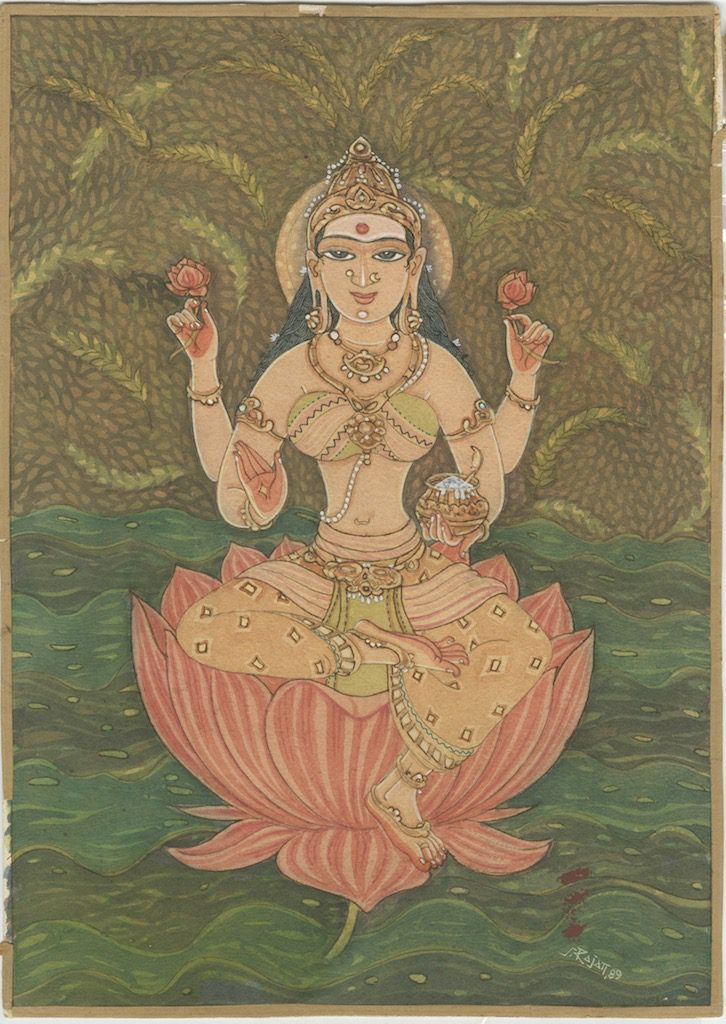
\includegraphics[width=0.8\textwidth]{pics/business1.png}
\caption{Devi Lakshmi who Rules over Wealth and Abundance}
 \end{figure}





 

\subsection{WEALTH INDICATIONS OF THE HOUSES AND THEIR LORDSHIP}
 

Houses of wealth and their lords are most important for income, whether we are considering the birth chart or muhurta (timing charts)

 

\begin{enumerate}
\item[*] The eleventh house and its lord gives good income, particularly that through our friends, associations and greater goals in life.\\
\item[*] The ninth house and its lord gives good luck, the favor of the government or other established authorities.\\
\item[*] The fifth house and its lord gives gain through speculation, like stocks and bonds, or good advice.\\
\item[*] The fourth house and its lord gives gains through property, vehicles and fixed assets.\\
\item[*] The second house and its lord shows gain through our own personal efforts or work we do with our own hands or with our speech.\\
\item[*] The tenth house and its lord gives social recognition, status and prestige.\\
 \end{enumerate}

Houses of poverty and their lords should not be prominent.

 

\begin{enumerate}
\item[*] The twelfth house and its lord gives high expenses and causes loss.
\item[*] The sixth house and its lord gives enmity, legal difficulties and disease.
\item[*] The eighth house and its lord creates obstacles, oppression and alienation.
 \item[*] The tenth house and its lord gives social recognition, status and prestige.\\
 \end{enumerate}

The lords of the third, sixth and eleventh houses can make us aggressive and cause us to act too hastily and without the right foundation. Hence, initial success may be followed by a fall. This is particularly true of the lords of the third and sixth. The lord of the eleventh may give wealth but we may be too impulsive or aggressive in using it and may lack the ethical outlook to make it a positive force in the world.

           

Planets that rule houses of wealth are strong if they are placed in their own signs or exaltation. They are also strong if placed in an angle from the Ascendant or the Moon. The lord of the eleventh in the tenth house is good for income through career. It is additionally good if they have an exchange or association with the Lord of the Ascendant. The lord of the second with the ascendant lord is good for income through ones work.

 

There should be associations or exchanges between the lords of houses of wealth. The lord of the ninth, for example, is good in the eleventh and the lord of the eleventh is good in the ninth. This gives good luck and favor from authorities. The lord of the second in the eleventh is good for income through ones work, as is the lord of the eleventh in the second. The lord of the fifth in the eleventh shows income through stocks or speculative ventures, as does the lord of the eleventh in the fifth. The lord of the fourth in the eleventh is good for property income, as is the lord of the eleventh in the fourth. 

 

There should not be exchanges between the lords of houses of wealth and those of houses of poverty. If the lord of the second is in the twelfth and the lord of the twelfth is in the second, this is a strong yoga for poverty. Similarly, it is not good if the lord of the sixth is in the fifth or the lord of the fifth is in the sixth, or if the lord of the ninth is in the eighth or vice versa.    

 

\subsection{INDICATIONS OF HOUSES FOR FINANCIAL GAIN}

 

Houses that give wealth should be strong, tenanted or aspected by benefics, and their lords should also be strong. Houses that give poverty should be untenanted.
Aspects of separative planets (Sun, Mars, Saturn, Rahu and the lord of the twelfth) should be avoided on houses of wealth, particularly on the tenth house that governs career.
 

\begin{enumerate}
\item[*] Planets in the eleventh give abundance, the realization of our aims and good income.

\item[*] Malefics like Saturn, Mars and the Sun do particularly well here for financial purposes.

\item[*] Benefics in the ninth give good luck, fortune and favor in legal ventures, particularly Jupiter, but malefics are to be avoided here.

\item[*] Benefics in the fifth give gain through stocks and speculative ventures, particularly Jupiter. Malefics here also cause harm.

\item[*] Planets in the fourth give property and vehicles. Saturn here is also good for this.

\item[*] Benefics in the second give good income through our own personal work but malefics can cause difficulty. Both Jupiter and Mercury do well here.

\item[*] Planets in the tenth, benefic or malefic, give us the power to influence the public but Saturn here often raises us up only to take us down again. 
 \end{enumerate}
 

Planets should not be located in houses of loss. Planets in the twelfth will give high expenses. However, if we are engaged in some charitable ventures we may have benefics or well placed planets in the twelfth. We should also note that some people who have both high income and high expenses will have a prominent twelfth house but other strong wealth- giving houses to balance it out. Venus in the twelfth, however, is generally good for wealth. The twelfth as the house of foreign countries can also show material activities in foreign lands, including import/export.

Planets in the eighth also give such financial difficulties. However, in insurance and inheritance matters, well-placed planets here are helpful.

Planets in the sixth give legal difficulties, enmity or conflict.  But well placed planets in the sixth, like Jupiter, Mercury or the Moon are often found in health or service ventures.

 

 



\subsection{THE MOON AND OUTER VENTURES: ISSUES OF TIMING}
 

Now we will examine broader issues of the influence of the Moon on financial ventures, mainly relative to timing, but these factors are helpful to know relative to the birth chart also. The Moon represents our capacity to influence people, to have an impact upon society, to reach the masses or large numbers of people. It gives popularity and recognition and keeps us in harmony with the trends of the time. Hence, for business ventures, particularly those that aim at the public or whose concern is teaching or communication, a strong Moon is necessary.

 

In addition, the Moon governs the birth or the first phase of all ventures. A strong Moon is important for the time of initiating important enterprises. It continues to rule them until they are off the ground (out of the womb as it were).

 

For timing of actions or decisions generally, the Moon should preferably be waxing. Generally, it should be between three days after the new Moon and full. The eleventh day of the Moon is best. The day of the full Moon is also good, preferably before the moment the Moon has exactly reached full.

 

The Moon in cardinal signs is better for starting ventures and provides more initiative and dynamic expression. It is better for ventures that aim at leadership, introducing new ideas or having a strong expression and influencing people. In fixed signs, the Moon is better for giving continuity and endurance to our projects. It is better for long term projects, fixed assets or property. In mutable signs, the Moon functions for reexamination or reformation of projects or working out their details. It is also better for matters involving communication or transaction of commodities and can be helpful for intellectual or artistic ventures.

\subsection{THE MOON IN SIGNS}
 

The Moon should reside in favorable or friendly signs. Cancer and Taurus, its own sign and sign of exaltation, are generally good for all enterprises. Cancer is better for matters involving the public or social influence, affairs of the home or personal communication. Taurus is better for those involving material resources, including articles of luxury such as gemstones.

 

\paragraph{THE MOON IN ARIES} is good for starting new ventures, particularly those dealing with science or the mind. It is good for projects that are inventive and are opening up new ground. It is more a time to develop new ideas, however, than to begin practical actions or to set up shop. It is better for projects promoting oneself or a particular personality. One must beware of being overly impulsive as it is not entirely wise to trust ones instincts at this time. One can be headstrong and too aggressive under its impulse.

 

\paragraph{THE MOON IN TAURUS} is good for artistic ventures or for businesses aiming at comfort and luxury. It is good for business partnership, particularly between husband and wife. It is good for dealing with fixed assets. It is also good for poetry, film and other affairs of Venus.

 

\paragraph{GEMINI MOON} is good for communication, writing and teaching ventures. It is good for educational pursuits, commerce, exchange of ideas, information and commodities generally but it is a fluctuating influence that is not always good for fixed enterprises or starting companies. Nothing should be trusted under its impulse unless it is done in contract.

 

\paragraph{CANCER MOON} is good generally for expressing our ideas and feelings to other people. It is good for healing enterprises, for food or domestic concerns and for influencing others generally and working with the masses. It requires that we are sensitive to public opinion, however.

 

\paragraph{LEO MOON} is good for projecting the power of our personality, for ventures having to do with the projection of our own will, character, fame, influence, status or honor or those of some personality. It gives good P.R. but requires that we take a leadership role. It will draw attention to us personally and we should be ready to deal with that. If afflicted, it can cause some negative notoriety.

 

\paragraph{VIRGO MOON} is good for healing, writing, art, crafts, sports, science and service ventures. It is one of the best Moon positions for getting to the details of practically establishing something. There is some danger of getting too caught in details, however. Hence, it is often better for finalizing rather than making initial decisions in a project. It is better for modest ventures than for great projects and by its mutable disposition may give ups and downs and make it difficult to maintain a long-term venture.

 

\paragraph{LIBRA MOON} is good for artistic, spiritual and political affairs. It is appropriate for new ventures designed to change or reform the world and communicate values of harmony and justice to the masses. It gives diplomacy and the capacity to influence people on a subtle level. There may, however, be a danger of being overly idealistic or fanatical. There may be impracticality, as ideas become more important than actual resources. It is also good for projects relating to Venus, like art.

 

\paragraph{SCORPIO MOON} is generally unfavorable for business matters, as it shows emotional confusion, domination and manipulation. It may cause conflict, emotional entanglement and legal problems. However, if its fall is canceled, it can be good for shamanism, psychology, astrology, religion, poetry, healing and scientific research.   

 

\paragraph{SAGITTARIUS MOON} is good for legal enterprises, for projects with religious groups, for working with governments, or with ones ancestors and their traditions. It gives clarity and order in action. It is good for establishing our principles and values. It is also favorable for travel. It is warm, friendly, expansive and optimistic but can attempt too many things.

 

\paragraph{CAPRICORN MOON} is good for influencing society, for establishing institutions, for working with traditions. It is often political. It gives objectivity and detachment, as well as the capacity to orient material resources. It is a good place to have the Moon to make business decisions, issues of money or property, but may lack in vision or sensitivity to the views of others. It is better for long term ventures or those slow to develop because the influence of Saturn will slow things down but make them strong in the long run. It is good for property and other affairs of Saturn.

 

\paragraph{AQUARIUS MOON} is usually not favorable for outer ventures. It gives faith, renunciation, dependency, and otherworldliness. Well‑placed, it is good for religious and spiritual enterprises and gives a capacity for group action. In this way, it can be good for charities and humanistic work. It is better for following than leading. It may cause us difficulties beyond our control or obstruction from friends or allies. It may indicate unrealistic ideas or expectations or show a venture with an inherent negativity and self-destructiveness. On a lower level, Aquarius Moon may get us involved in underworld dealings, like drugs or other forces of deception and illusion.            

 

\paragraph{PISCES MOON} is good for art, imagination, enthusiasm, and intuitive ventures, as well as for affairs involving the sea or commerce across the sea. It is creative and good for establishing new motivation but lacks in objectivity and consistency. It gets carried away by moods, whims or enthusiasm. Hence, it requires careful scrutiny. It is often too fluctuating to be trusted.

 

When judging the position of the Moon in signs, we should also consider that of the ruler of the sign in which the Moon is located (its dispositor). It should also be favorably placed, particularly relative to the Moon, and be in a friendly relationship to it.

\subsection{ASPECTS TO THE MOON}
 

The Moon should be free as much as possible of unfavorable aspects. Conjunction with Rahu, the north lunar node, creates false imaginations and unrealistic plans. It may get us carried away by unreliable mass trends, or though our business may be successful its spiritual and psychological complications may prove difficult or unwholesome.

 

A little influence of Saturn on the Moon may be good as it gives objectivity, but very much can give negativity, an overly conservative nature and the inability to make use of opportunities. Outwardly it can give obstructions and result in loss.

 

Aspects of Mars to the Moon can cause impulsive or rash action and can show conflict or legal difficulties. Problems of communication with the public may arise. Ketu, the south node, causes contraction and may give difficulties or obstructions beyond our control, including conflict or contradictory situations.

 

The best aspect to the Moon is a good influence of Jupiter. Aspects of Jupiter or Jupiter in an angle from the Moon, particularly if Jupiter is exalted or in its own sign, are good. Jupiter gives expansiveness and success, and usually right values, as well as the favor of legal, business and government influences.

 

Aspects of Mercury aid in proper communication and exchange of information. This is useful in all ventures but particularly affairs of teaching or communication. Mercury in itself, unless it is the ruler of houses of income, however, may not be strong enough to give success.

 

Venus gives charm and ability to influence and is usually helpful in gaining resources for us. Its influence is good for artistic matters or projects involving women.

 

\subsection{THE MOON AS HOUSE LORD}
 

The Moon should be the lord of favorable business houses from the ascendant. Favorable ascendants in which the Moon rules positive houses for business are: Aries (4), Gemini (2), Cancer (1), Virgo (11), Libra (10), Scorpio (9), Capricorn (7), and Pisces (5). If not the lord of good houses, the Moon should be well placed or well aspected to compensate for this.        

 

\begin{enumerate}
\item[*] For Aries ascendant the Moon, as ruler of the fourth house, gives property, domestic or emotional happiness.
\item[*] For Gemini, as ruler of the second, it gives income and gains in ones personal occupation.
\item[*] For Cancer, as ruler of the ascendant, it furthers all enterprises generally and exalts ones personality.
\item[*] For Virgo, as ruler of the eleventh, it gives good income and high values.
\item[*] For Libra, as ruler of the tenth, it gives fame, status and social recognition.
\item[*] For Scorpio, as ruler of the ninth, it gives good luck and favor of government, spiritual or religious groups.
\item[*] For Capricorn, as ruler of the seventh, it gives political and social power and capacity to work with partners.
\item[*] For Pisces, as ruler of the fifth, it gives gain through children, creativity, speculation and good advice.
\item[*] For Taurus, as ruler of the third, the Moon gives energy and curiosity but not always good business sense. The individual may be too impulsive to be successful.
\item[*] For Leo, its function depends upon the planet which most influences it as it is lord of the twelfth. By itself it gives loss.
\item[*] For Sagittarius, it gives capacity for profound thinking but not always practical sense, though it is good for inheritance. Again, its value depends a lot upon how it is influenced as ruler of the eighth which also has a neutrality to it.
\item[*] For Aquarius, it is good for service or healing work, but not so much for income or commercial ventures and may give legal problems, as it is ruler of the sixth.
 \end{enumerate}


\subsection{THE MOON IN HOUSES}
 

In terms of house location, the Moon is best placed in angular or trine houses – 1, 4, 5, 7, 9 & 10 – as these give it strength. The fourth house is the strongest as it has directional strength as well.

 

However, the Moon can also be good if it is located in houses of income like 2, 5, 9 & 11. It is excellent if it is located in angular houses as the lord of a house of income; for example, the Moon in the tenth house as lord of the eleventh, as for Virgo ascendant is very good. It is also good if it is exalted or in its own sign in a house of income; for example, the Moon in Cancer in the eleventh for Virgo ascendant, or the Moon exalted in Taurus in the eleventh for Cancer ascendant.

 


\subsection{JUDGING MOTIVATION}

For integrity in business ventures, the Moon should be associated with the lord of the ninth from the ascendant or with sattvic planets like Jupiter and the Sun. Mercury should similarly have sattvic influences. Mars and Saturn should not be too strong or in association with each other. Combinations of Mars and Venus are also to be avoided as they accentuate the emotional nature.


\subsubsection{OUTER INDICATIONS OF OTHER PLANETS}
Once the Moon is strong and under good influence, it is important to examine the other planets which govern business ventures.

 

\paragraph{MERCURY }

A good Mercury is necessary for the proper communication which all enterprises depend upon. It governs the second stage of ventures, when we are in a position to communicate them to others and do commerce through them. It gives ease in the exchange of commodities and ideas. It is also particularly important for affairs dealing with communication, writing, teaching, and healing.

 

It is better if Mercury is not retrograde, or in conjunction with the lunar nodes (unless in its own sign). Nor should it be within two degrees of the Sun, as this blocks objectivity.

 

Mercury conjunct or aspect Jupiter is very favorable and gives practical gains. Jupiter gives expansiveness and Mercury the ability to influence others through it. Mercury with Venus is good for creative or artistic pursuits. Mercury with Saturn is all right for property or for serious mental pursuits but otherwise not good. It makes one materially conservative. Mercury with Mars is good for scientific or legal ventures but is apt to make one overly aggressive.

 

Mercury should not be debilitated which gives immaturity and foolishness, or at least impracticality. Its better signs for location are Taurus, Gemini, Leo, Virgo, Libra, Capricorn, Aquarius, which are those of its friends. It is better located in houses 1, 2, 4, 5, 7, 9, 10 & 11. Mercury is a very strong wealth-giving planet for Leo ascendant as  it rules two houses of wealth, 2 and 11.

 

\paragraph{JUPITER}

Jupiter is the main planet that gives wealth, hence he should be favorably placed and aspected. Jupiter governs the main phase of any activity, when its greatest expansion and success occurs. It gives optimism, the capacity for action and strong endurance. It is good for all business enterprises particularly where there are legal, government or religious groups to deal with. It is good for all charitable ventures as well.

 

Its better signs are Aries, Cancer, Leo, Scorpio, Sagittarius, Aquarius and Pisces. Jupiter is a strong wealth-giving planet for Aquarius by the dual houses of wealth it rules, 2 and 11. It is better located in houses like that given under Mercury, particularly in its own sign or exalted. Jupiter in air signs is good for knowledge but not always for the holding of wealth.

 

\paragraph{VENUS}

Venus gives the charm and charisma necessary to carry out most ventures relating to the public. It is good for enterprises that depend on quality, taste and high values, rather than mass marketing. It is good for businesses involving women or products aimed at them. It is good for vehicles as well. It is essential for artistic and creative ventures. Venus gives wealth and luxury but not always motivation, the urge to work, willingness to do service or great generosity.

 

\paragraph{SATURN}

Saturn shows the obstacles we have to face in our endeavors. It indicates the time that may be needed to accomplish them. It gives property and enduring status but only after persistent effort and often many ups and downs. It may raise us up but can also bring us down, particularly if our actions are selfish.

 

It is usually not favorable to have Saturn in the tenth house, particularly by itself, in any career venture. It does well in the eleventh, however. It is mainly good for property. A strong Saturn is also helpful for working with the government or other institutions and organizations.

 

\paragraph{MARS}

Mars shows the energy and motivation that we have to accomplish things. Well placed, it gives leadership, decisiveness, dynamism and inventiveness. Misplaced, it can make us reckless or too forceful in our actions and bring us into conflict or legal complications.

 

Mars is better for scientific and technical ventures. It gives logic as well. A strong Mars is good for legal affairs, but may cause us to push things too far.

 

\paragraph{THE SUN}

The Sun shows the power of our will and character we have to rely on, or the authority we are able to create. It gives us honor, respect and prestige and often gives the good grace of the government or whatever powers we are looking up to.

 

It does not do well in the second house, however, as it can show high expenses. Its malefic affect on houses should be considered. It is particularly important for ventures that depend upon a strong force of character and individuality, which require a famous or well recognized personality.

 

\paragraph{RAHU, THE NORTH NODE}

Rahu shows our greatest desires. It indicates our area of greatest success, on one hand, and our area of most unrealistic expectations, on the other. It is usually not to be trusted, though it can be a source of many good ideas that need to be validated by other sources.

 

Well placed, as in the tenth house, it can give great success, particularly with the public, as with mass media ventures or communication projects. It sometimes does this if located in other angles like the seventh and the first. It is usually good for income if placed in the eleventh or for good fortune if placed in the ninth. In the sixth it can be good for success in legal ventures. As usual, we must always consider the strength of its lord and the houses its lord rules.

 

\paragraph{KETU, THE SOUTH NODE }

Ketu shows our hidden resources, our psychic reserve. Yet for outer ventures it causes negativity and doubt. Only with planets in their own or exaltation sign does it become a powerful augmenting force and will tend to magnify whatever influences they possess. Ketu with the lord of the second or eleventh houses in their own sign or exalted is particularly good for wealth. This is especially true if the planet involved is Mercury or Jupiter.

 
\subsection{PLANETARY PERIODS}

 

Once the Moon and the other planets are strong and under good influences, we have to consider the dashas or planetary periods. The planetary periods of the birth or horary charts should be given their proper attention. Even if the chart is good the results cannot be gained if the period is not right for it.

 

We should note the major and minor planetary periods governing the time of the chart. These should be of planets that can give wealth, like Jupiter, Venus or Mercury, or of the rulers of houses of wealth like the second, fifth, ninth and eleventh. Generally, a combination of periods of lords of different houses of wealth is very good. For example, if the major period is of the lord of the tenth house, the minor period of the lord of the second, the subminor the lord of the ninth, it should be very good. If on top of this there is a good transit of Jupiter, the period becomes very strong.

 

Periods of the lord of eleventh house usually give income if well placed. Periods of the lord of the second are favorable for career gains. Periods of the lord of the fourth give property or vehicles. Periods of the lord of the ninth give good fortune, luck or sudden and unexpected gains.

 

Similarly, periods of malefics or malefic lords cause difficulties. The period of the lord of the twelfth house can give loss or high expenses (again consider the other house the planet rules). The period of the lord of the eighth gives adversity. The period of the lord of the sixth gives legal or health difficulties which have financial implications.

 

\subsection{SUMMARY}

 

It is difficult to find a birthchart or horary time that is entirely good for all these factors of wealth and prosperity. It is always the majority of factors that has to be considered. A strong birthchart is always a good foundation to work with and will yield good results over time (though not all the time). Then timing comes into play.

 

Then it is best to consider the length of the time period when a venture should be done. If it has to be started within a three-month period, then we look to the favorable positions available at those times by way of transit and choose the best. We can use astrology, particularly the birthchart, to see if the ventures should be started soon or whether one should wait. This depends upon the birthcharts of the people within the business.
\newpage

\section{RELATIONSHIP ASTROLOGY -
CHART COMPARISON: COMPOSITE READINGS}
 

One of the most important and common usages of Vedic astrology today is for compatibility. This extends from marriage and personal relationship to friendship and business issues. We will focus more on the relationship and marriage compatibility. Examining relationship potentials in charts is an important and complicated issue. Comparing two charts for their compatibility is one of the main things you will be asked to do as an astrologer as relationship is often the key issue in human life. We will examine these factors in this lesson.

 



\subsection{\textbf{We begin with an audio on Relationship Compatibility with Vamadeva that introduces the factors discussed in detail below}}

 

\subsection{GENERAL ISSUES OF RELATIONSHIP ANALYSIS}
 

\subsubsection{Hindu Versus Western Culture}

 

In traditional Vedic Astrology, charts of prospective marriage partners, generally young people whose marriages are being arranged, are judged for compatibility. This is the main emphasis of the astrological analysis of relationship in Vedic Astrology. In modern times, and in Western Astrology, charts are used to help work out issues in relationship, as well as to examine compatibility on different levels. With the ease of divorce and freer sexual relationships today, such relationship examinations are more frequent. Hence, this branch of astrology is different in the West today than it was in older India. It is used more broadly and astrologers will be asked to examine relationship potentials in most of their readings.

 

\subsubsection{Methods of Judging Compatibility}

 

There are a number of methods of comparing different charts for compatibility. Most of these focus on marriage. There are methods that compute compatibility factors, like favorable signs or Nakshatras (the kuta system that we will examine in the next lesson). They add up the various points and see if there are enough in common to guarantee a good match. Such calculations can be helpful but as they are based upon Indian marriage standards which are different from those in the West, we cannot expect them to work here without some modification. There are other methods that compare all relevant factors in both charts. While this second method is more complex, it is more detailed and more accurate so we will examine it first.

 

\subsubsection{Human Relationship Potentials}

 

Some of us have the idea that there is only one person for us in life. Most of the time, however, we have several relationship options on a number of levels. We come together for various reasons, some based on outer factors of physical or emotional attraction, others based on inner karmic or spiritual purposes. And inner and outer affinities can combine in different ways. Hence, we must strive to understand our general relationship potential rather than just fixate on one person we may happen to be involved with. Many people who are married more than once will be married to different types of people. We should see what planetary influences they are opening up to in each case.

 

Some individuals have powerful charts for relationship but may not find any one relationship that really works. Their strong relationship energy may draw them into different relationships. Other individuals have weak charts for relationship but may maintain a distant or detached marriage throughout life. Yet other types may have a life long relationship but out of inertia, not because there is real communication or compatibility.

 

In doing a comparative reading, a good deal of discretion is required. We should not just tell a client that they have a good or bad chart for relationship or that the chart of their potential partner is good or bad. As in all factors, we should not try to make decisions for the client. We should acquaint them with the positive and negative potentials available to them and allow them to make their own decisions. We must remember that relationship is an emotional issue and cannot always be approached along rational lines. We must approach our clients on this issue with the same tact with which we would expect someone to examine our own chart.

 

\subsubsection{Broader Issues of Compatibility}

 

It is not enough to judge compatibility emotionally or sexually. Issues of work, children and spirituality have to be brought into play, not to mention career which is so important today. Two people may love each other or have much in common but may not be able to live together. A certain harmony of style and daily action is required. We may also find a great deal of affinity between two charts. This, however, may not indicate marriage.  It may indicate friendship, a brother-sister relationship or a spiritual tie. In our culture we have a tendency to think that all male-female relationships should involve sexual activity. Hence, we may try to create a sexual relationship out of what is a relationship of another type. The astrologer should be careful not to turn what is an affinity, perhaps even profound, into something good for marriage or relationship, as this is not always the case.

 

Traditional Hindu astrology follows Hindu cultural values. These are of one life long marriage, no divorce, and having children as an essential part of marriage. Since traditional Hindu society is fixed and marriages are usually arranged, the rules for marriage from Hindu astrology are rather strict. We cannot follow that method in this country without modifications.

 

We must hold to the first principle of Vedic Astrology here as elsewhere – that the most important thing in human life is the development of consciousness. Relationship should be part of this but often it is against it. Hence, while we acknowledge the importance of relationship and the natural human urge towards it, we should give the other goals of life their due as well.

 

\subsubsection{Relationship and the Spiritual Life}

 

From the spiritual standpoint, marriage is not necessarily a good thing, nor is divorce necessarily bad, though it is usually very traumatic. If a relationship aids in the conscious growth of both people, it has its value. If it does not do so after a period of time, or if it obstructs inner growth, such a relationship may be better if it came to an end. However, many relationships can be successful even if only one partner is on the spiritual path. This requires openness on the part of the partner who is not on the path.

 

Relationship is always an individual matter that cannot be judged by general rules. We should aid our client in what furthers their aspiration in life and not just project social or religious standards upon them. Certainly marriage is a very powerful psychic tie that should not be entered into carelessly and which cannot be ended without considerable work and effort. Generally, we should only end a marriage relationship if it becomes a real block to spiritual growth, particularly if a pattern of unfaithfulness emerges.

 

If a marriage does not have children, if it is a second or third marriage or has lasted only a short time, it may be a weaker psychic link. We must examine its whole structure and not just place it under a category because of its name.

 

\subsection{COMPARATIVE READING OF CHARTS}
First we will begin by examining the relationship potential within the chart of each individual. On this basis we can better compare the two charts together, which is the second step.

 

\subsubsection{EXAMINATION OF THE INDIVIDUAL BIRTHCHART—}
 

It is best to examine both charts in a relationship issue, starting with each chart by itself. Often what may not be clear in one chart will be obvious in the other.

 

We can learn a great deal by examining the relationship potential and time factors within the individual chart itself. Even if we are doing some comparative analysis, we must start with this as a first step.

 

Determining the type of partner that is good for an individual comes in here. Through an individuals birthchart we see their general relationship potential, which may have several directions of application through different periods of time.

 

However, quite often we are attracted to the kind of partner who is not good for us, and we are not attracted to the partner who is. Our desire nature causes us to seek something new, sensational, or hard to achieve, which appeals to our illusions. We want a beautiful partner but not necessarily a kind or spiritual one. Hence, it is more a matter of living compatibility that we should seek, not necessarily how exciting the partner may be.

 

\subsubsection{ASTROLOGICAL FACTORS}

 

For the male, relationship potential involves examining the positions of Venus, the seventh house and its lord. For the female, it is the position of Jupiter, the seventh house and its lord. For both, the position of Mars should be examined, particularly with reference to Kuja Dosha.

 

Western Astrology considers Mars for the female. This is because western culture emphasizes marriage more as a sexual or emotional passion, as revealed through the Mars-Venus interchange. Vedic Astrology emphasizes dharma or principles of right living. This is seen by the Jupiter-Venus connection. However, in western culture we may have to give more emphasis to the role of Mars.

 

If a person has a highly afflicted seventh house and related factors, no matter how good the partner may be, harmony in marriage is going to be difficult.
So too, if a person has a very good seventh house and related factors, a successful marriage may be easy and may not require the perfect partner to succeed.
 

However, we have to examine the whole character of the chart, whether the person is introverted or extroverted, mental or emotional, spiritual or materialistic in orientation, and so on. Relationship must be based upon a harmony of spirit and values.

 

\subsubsection{PLANETS IN THE SEVENTH HOUSE}
Generally speaking, planets in the seventh house are not good for lasting relationship of a personal nature, though they may be good for public or social expansion, as well as for career.

 

THE SUN in the seventh causes separation and conflict, and while it orients the person towards relationship, the issue often becomes overweighed. The individual may be dependent, controlling or domineering, depending upon whether the Sun is strong or weak. They may use relationship to express their power potential rather than their own action in life. This position, however, is good for public and career work and can allow us to project a strong personality in these outer fields of life.

For women, the Sun in the seventh generally denies marriage. They seek relationships with married men or men beyond their status with whom it is not possible.

 

THE MOON is usually good in the seventh house, particularly for women, unless it is waning or poorly aspected. It gives the capacity for sharing, nurturing, caring, receptivity and sensitivity to others. It is also helpful for public and career issues as it gives the ability to influence people. It can, however, get a person caught in relationship or the social mind. Or it can make the person too emotional about relationship issues.

 

MARS is difficult in the seventh as it creates conflict of will, aggression and possibly even violence. Relationships are apt to be turbulent, dramatic and the individual may insist upon their own point of view. The individual may have a strong impact on others and wield power in society but is often not capable of lasting personal affection. Yet I have seen a number of charts with Mars in the seventh and a life-long marriage. This usually requires that both partners share some work in the world together, are both very achievement oriented, or that one surrenders to the will of the other. These factors serve to neutralize Mars.

 

MERCURY gives a good capacity for communication when it is located in the seventh house. They can relate easily to other people, particularly members of the opposite sex. Yet relationships are apt to be hasty, superficial or transient. Often an early unsuccessful marriage is indicated. The individual may enter into close relationships too quickly or easily. There may be much nervousness and volatility in relationship. Relationships with younger people are often indicated. This position is also good for career, business, communication or writing.

 

JUPITER is generally good in the seventh and gives the basis for a spiritual or dharmic relationship. It shows a loyal, ethical and honest approach to relationship. It gives friendship, happiness, compassion and a longing to share ones activity in life. It is also good for public and career work, which the partner may share. It shows a positive will in relationship and partnership. However, even Jupiter in the seventh can cause difficulties because it can make the person too expansive in relationship or apt to sacrifice their relationships to their principles.

 

VENUS is not always good in the seventh, as it can indicate an overly strong sensuality or sexuality. It does give a proclivity for love, passion and romance. For women, it renders them beautiful, attractive or sexy and usually keeps them in relationship. For men, it is not always good as it can make them feminine or passive but it may give them a beautiful wife. It also gives artistic capacities, like painting or dance. In its own sign or a sign of Mars, it gives a strong sexual nature.

 

SATURN is generally not helpful for relationship in the seventh. It causes separation, alienation and loneliness. The individual may be too introverted or self-involved to relate to others on an intimate level. Conflict, separation or rejection can occur. It also can make us prone to unusual sexual activity, as for example homosexuality. Well placed, however, it can indicate one long-term or life long relationship. Like Jupiter, it is also good here for public or career influence and additionally has its directional strength in this house. It also gives us relationships where there is an age difference. Usually this gives older partners for women and younger partners for men.

 

RAHU causes its typical difficulties and confusions here. Relationships may be superficial, based on a following of external influences or momentary whims. There may be much projection, unrealistic desires and some unwholesome fantasies. There may be strange psychic experiences in relationship. Much depends upon the planet that rules Rahu and some power of influence for career may come from this position. Rahu when strong here can be good for career, like its influence in the tenth house.

 

KETU causes a critical and contracted manner in relationship. The individual may be strongly introverted, eccentric and self-involved. Psychic conflicts may occur, with hidden power issues. Accidents or difficulties may occur in relationship. Again, the planet that rules Ketu should be consulted. Ketu can give a psychic or spiritual partner.

 

A combination of planets in the seventh should be judged by the nature of the planets involved and their house rulership, but generally the more planets are in this house the more difficult for relationship it will be. While a number of planets in the seventh can be good for social prestige, unless they are benefics, they prove difficult for relationship. Combinations of the Moon and Jupiter, with possibly Mercury or Venus are good. Combinations of Mars and Saturn cause many difficulties, if not perversion and violence. These are compounded if the lunar nodes are involved.

 

Malefics exalted or in their own signs in the seventh give much power in life, but still cause difficulties in relationship. For example, a woman with Mars in Aries in the seventh will have a strong will and achievement potential, often good business capacity, but will have difficulty in relationship, particularly on an intimate personal level.

 

\subsubsection{ASPECTS TO THE SEVENTH HOUSE AND ITS LORD}

 

Aspects of malefic planets (the Sun, Mars, Saturn, Rahu, and Ketu and the lords of the sixth, eighth and twelfth) to the seventh house or its ruler tend to cause separation or divorce. The Sun will make us too individualistic or dominating. Saturn will make us too contrary, solitary or fearful. The aspect of Mars can cause conflict or sorrow, and is a factor in Kuja Dosha. Rahu will give us unrealistic expectations and confusion of motivation. Ketu will make us defensive and contracted. The lord of the twelfth will cause us to negate relationship. The lord of the eighth or sixth houses can also be difficult here, not only for relationship but for health.

 

On the other hand, aspects of benefics boost up the seventh house and its effects. Best on the seventh or its lord is the aspect of a benefic Jupiter. It can guarantee happiness in relationship. It creates understanding of the partner and good will in relationship. It is particularly strong if Jupiter is also ruler of the seventh. The aspect of the Moon is generally good unless the Moon is waning and afflicted. The Moon gives a capacity to communicate and sensitivity of feeling, a general openness and sharing.

 

The aspect of Venus to the seventh house is helpful for giving affection and for making the individual attractive. The aspect of Mercury to the seventh house increases communication but does not guarantee lasting contacts.

 

The aspect of the lord of the seventh house to the seventh house that it ruels is usually helpful, unless it is a malefic. But even this is not always good if it comes from the first house, which can show the seventh lord limited to the sphere of the self (first house).

 

\subsubsection{DISPOSITION OF THE LORD OF THE SEVENTH HOUSE}

 

The lord of the seventh should be strong and well-aspected. Placed in the first house it can weaken relationship by keeping us focused on ourselves or on our own work in life. In this case, the indicator of relationship remains in the field of the self. The lord of the seventh in the first house is common in the charts of people who dont marry.

 

In the second house, the seventh lord can cause us to treat relationship as a function of work or livelihood. It also can give income or material advance through relationship. But it can show harm to the partner as it is the eighth house from the seventh.

 

Placed in the third house, the seventh lord can make us independent and impulsive in relationship. In the fourth, it is usually good for marital harmony and shows a receptive mind. It is particularly good for women. In the fifth, it gives a strong romantic nature and possible love marriage. In the sixth, it can indicate a sickly partner, difficulties in relationship, or some work with the partner.

 

In the seventh, it is good socially but not necessarily personally and should be judged by its nature. The lord of the seventh in the seventh is good for benefics like the Moon, Mercury, Venus and Jupiter. It is not good for malefics like the Sun, Mars and Saturn unless they combine with or are strongly aspected by benefics.

 

The lord of the seventh in the eighth can give health problems through relationship or loss through the partner, sometimes the loss of the partner. In the ninth, it is usually good and shows a spiritual or dharmic connection, or grace through the relationship.

 

In the tenth, it shows a prominent or powerful partner, with whom one may share ones career or possibly work for. In the eleventh, it shows more than one marriage and strong goals or gains through marriage. In the twelfth, it can indicate secret pleasure or secret sorrow in partnership.

 

\subsubsection{EFFECTS OF OTHER HOUSES OF RELATIONSHIP}

 

The seventh is not the only house of relationship. The fifth should be consulted as the house of love, romance and children. We should note the planets here and the aspects to this house and its lord like the seventh. An exchange between the lords of the fifth and the seventh indicates a love marriage. The twelfth is another house of pleasure. Venus here, for example, often gives a strong sensual orientation. Mars or Venus in any of these houses, particularly if they are signs of Mars and Venus, or if the two planets aspect each other, give a strong sexual nature.

 

\subsubsection{OTHER PLANETARY POSITIONS}
Besides the disposition of the seventh lord and seventh house there are other planetary positions that have important bearings on relationship.

\subsubsubsection{SUN AND MOON}



 

The Moon represents the general social and emotional capacity of a person. A good Moon is helpful for good relationships. Specifically, the Moon in a mans chart represents his general capacity to relate to women. This should be examined for long term and general marital and domestic happiness. With a weak or detached Moon the man may not have the patience for a long-term relationship.

 

The Sun similarly represents the woma’ns general capacity to relate to men. A weak or afflicted Sun may not give her the openness to male energy necessary for a happy relationship. A woman with a weak Sun will often choose weak men as partners, as will a man with a weak Moon.

 

\subsubsubsection{MARS AND VENUS}

 

For marital or sexual issues, it is important to note the relationship between Venus and Mars in the chart. If Venus and Mars are in close aspect or mutual reception, this gives a strong sexual drive. This is particularly true if they are in fixed signs or in houses of sex (the fifth, seventh, eighth or twelfth). A strong sexual drive, however, is often not conducive to marital happiness, though it projects us into relationship. This is because it causes us to seek additional fulfillment outside of marriage (it is promiscuous).

 

\subsubsubsection{KUJA DOSHA}

 

Mars in certain houses creates difficulties for harmony in marriage and relationship. Some Vedic astrologers take these very seriously, others do not. Generally north Indian astrologers weigh them more heavily than those in the south.

 

Kuja Dosha occurs if Mars is in houses 1, 4, 7, 8 & 12.
Exceptions occur in house 1 if the sign is Aries, house 4 if it is Scorpio, house 7 if it is Capricorn or Pisces, house 8 if it is Cancer and house 12 if it is Sagittarius.
 

Such a placement shows potential conflict in relationship or a negative impact on the life of the spouse. A person with such a planetary placement should generally only marry another person with a similar placement. A too strong Mars in the chart of a woman is particularly difficult for marriage from the Hindu point of view as it would make her dominate her husband and perhaps cause him ill health or even death in extreme cases. Such placements should not be interpreted too simplistically since over one-third of charts have them to at least some degree. I consider Kuja Dosha but dont weigh it too heavily. It is more an issue if Mars is in first, seventh or eighth. Then the other partner should have some form of Kuja Dosha to be on the safe side.

 

\subsubsection{PLANETARY PERIODS}

 

Marriage or close relationship, even if indicated in the chart, may not occur until a favorable planetary period or subperiod comes. If the chart is generally good for marriage but the planetary period if of an adverse planet, this may cause delay or difficulty. Different types of marriage or different marriages will be reflected in the different planetary periods in operation at the time.

 

\subsubsubsection{Results of Planetary Periods}

 

\begin{enumerate}
\item[*] Favorable periods for marriage are those of the lord of the seventh, planets in the seventh or which aspect the seventh (if they are not malefic), planets which are with the lord of the seventh or aspect it (again if they are not malefic).
\item[*] The period of VENUS is generally favorable for marriage, particularly in the minor period of the lord of the seventh. JUPITERS period is also usually good, particularly for women.
\item[*] Periods of SATURN are usually difficult unless it is the lord of the seventh. Saturn in the seventh may not give relationship during its period. Saturns period often gives partnerships with an age difference between the individuals involved.
\item[*] Periods of RAHU naturally bring marriage but it is not always or even usually successful unless well placed. It can bring marriage with a foreigner, with someone with whom there is much illusion and may not last beyond its period.
\item[*] KETUS period is generally not favorable for marriage but can bring marriage if it aspects the seventh. Such marriages seldom last beyond the period of Ketu. Again, we have to consult the rulers of these planets.
\item[*] The period of MARS is also usually not favorable for relationship, particularly for women, unless it is lord of the seventh. Mars major, Venus minor periods (or vice versa) are often very strong for relationship but usually bring romance or sexual encounters rather than marriage.
\item[*] The period of MERCURY is mixed in terms of relationship. It often gives early marriages as lord of the seventh, particularly if its period comes young. If it comes when we are older, it often gives relationships with younger people.
\item[*] The period of the SUN is more favorable for marriage for women, particularly when it is lord of the seventh or the fifth.
\item[*] The period of the MOON is generally favorable for marriage, particularly as lord of the fourth, fifth and seventh houses.
\item[*] The period of the seventh lord tends toward marriage. So do the periods of planets located in the seventh house or planets aspecting the seventh house or its lord both in the birthchart and in the navamsha.
 \end{enumerate}

\subsubsubsection{Varshaphal or Annual Chart}

The Varshaphal or annual chart indicates marriage by good planets in the seventh house or aspecting the seventh house or seventh lord with favorable aspects. The same is true of positions from the Moon. Strength to Jupiter and Venus also helps.

 

\subsubsubsection{Transits}

Transits of planets should also be considered, particularly the slower moving ones like Saturn and Jupiter. When Jupiter and Saturn both influence the seventh house or its lord, marriage is more likely. When a person is at the age for marriage, we should see when the most favorable planetary configurations are likely to occur.

 

\subsection{INDICATIONS OF INCOMPATIBILITY}
 

There are also factors in the individual chart that show difficulty in relationship or non-suitability for partnership.

 

\subsubsection{FACTORS OF DETACHMENT FROM RELATIONSHIP }

 

Other factors of detachment from relationship or emotion should be considered as negative factors for relationship. These include Saturns influence on the Moon or the Sun, particularly their conjunction that makes a person more prone to a life alone or to becoming alienated from others. Saturns influence on the second, fourth, seventh or twelfth houses and their lords promotes detachment as these are houses of personal happiness and relationship. The Sun or Moon with Rahu or Ketu are similar patterns of disruption in relationship or personal identity. Saturns influence on Venus is another consideration, though this may only delay relationship.

 

Such factors as Venus or the Moon in Saturnian signs may be noted as well. Yet these things may cause a detached marriage or an intellectual, spiritual, work or social relationship rather than a domestic or romantic connection.

 

\subsubsection{CHARTS DANGEROUS FOR THE PARTNER}

 

Some individual birthcharts may not only not be good for relationship, they may threaten the life, health success, or well-being of the partner. This was the basis of the Kuja Dosha or the difficult placement of Mars. Such factors include all the issues of Kuja Dosha. They include malefics in the eighth house, like Mars, Rahu, Ketu or Saturn or the lord of the seventh in the eighth house.

 

For example, the chart of a client who had contracted AIDS had Gemini Ascendant with Jupiter, the lord of the seventh, at its maximum degree of debility in the eighth house in Capricorn. This person lost many partners to the disease.

 

If a woman has a very strong Mars, it may prove difficult for the partner, unless his Mars or Sun is very strong. If a woman has a strong Sun, it does not threaten the life of the partner but may repel potential partners. Similarly, a man with a very weak Mars or Jupiter may not be helpful to a woman. A weak Mars will not give him enough courage in life. A weak Jupiter will give him misfortune. We must always remember that whoever we enter into partnership with, we tend to take on the karma in their birthchart.

 

\subsection{2. COMPARISON BETWEEN INDIVIDUAL CHARTS—}
 

After having thoroughly examined the individual chart for its basic relationship potential, we can begin our comparison of the individual charts involved. First, we should examine the chart of the partner the same way and see if the factors for relationship are similar, or if the chart of one or the other will compensate for or augment the difficulties in the charts of the other.

 

Generally, we are attracted to someone different than ourselves. We are not seeking to be married to ourselves. Hence, it is not always good if the charts are too much alike. On the other hand, the two charts must have enough in common to be able to communicate. There should be a balance of corresponding and complimentary factors, like the interchange of masculine and feminine planets.

 

Above all, there should be a sharing of primary goals in life. A person of spiritual bent should be careful in marrying a person of commercial disposition, for example. The long-term compatibility of values and daily activity is more important than short term infatuation. Issues of children, finance and work should be examined as well. Even strong emotional or spiritual ties may not be enough if these issues are not in harmony.

 



 

\subsubsection{EXCHANGES BETWEEN PLANETS}
 

Particularly important are the exchanges of male and female planets between the two charts, mainly the Sun and the Moon and Mars and Venus. The Sun in one chart may be conjunct the Moon in the other, for example.

 

\subsubsubsection{Sun and Moon}

 

Generally, the woman surrenders her Sun to the man and the man surrenders his Moon to her. We can see from a womans Sun how she relates to men generally. Its connection with the Sun of her partner shows us how she relates her partnership potential to him. Similarly, we can see from a mans Moon how he relates to women generally. Its connection with the Moon of his partner indicates his female relationship potential generally.

 

Exchanges of the mans Sun with the womans Moon show a deep harmony of will and emotion. Such exchanges of luminaries, however, do not guarantee a marriage relationship. They show the potential for deep friendship and sympathy and are also often found in the charts of brothers and sisters, fathers and daughters, mothers and sons or any close human tie.

 

An exchange of both luminaries, when the Sun in one chart is conjunct the Moon in the other and vice versa, gives a very strong affinity of characters.

 

A similar affinity may be created when the Sun or Moon in one chart conjuncts the ascendant in the other. It is also good if the luminaries are opposite each other in the chart.

 

\subsubsubsection{Venus and Mars}

 

Mars and Venus show how we project our sexual energy. Venus in a mans chart shows how he projects his sexual energy onto women. Mars in a woman’s chart shows how she projects her sexual energy onto men.

 

Exchanges of Mars and Venus, particularly the mans Mars with the woman’s Venus give a very strong sexual attraction. This, however, is not always good for marriage. It may give a sexual attraction that blinds the person. Where the rest of the chart is not compatible, it can cause many difficulties. Yet where there is compatibility in the chart it can be an important aid in making the relationship stronger. Without some Venus-Mars attraction relationships may be of a more friendship or familial nature.

 


\subsubsubsection{Venus, Sun and Moon}

Venus-Sun exchanges are generally good for male female relationships. The woman’s Venus on a mans Sun is very helpful. The woman”s Moon or Venus on the mans Venus or Moon is also good.

 


\subsubsubsection{Mars, Sun and Moon}

Mars exchanges or aspects on the Sun and Moon, however, are not favorable. A mans Mars on a woman’s Moon is particularly difficult and causes emotional disharmony and conflict.

 


\subsubsubsection{Jupiter Exchanges}

Jupiter-Venus or Jupiter-Mars exchanges between charts are also good. They show an alliance between Dharma (Jupiter) and Kama (Mars and Venus). A womans Jupiter on a mans Mars or a mans Jupiter on a womens Venus are excellent for compatibility.

 

 


\subsubsection{HOUSE INFLUENCES}

 

It is important to compare how the planets in one chart affect the houses in the other. This we can see by using the ascendant in one chart for reorienting the houses in the other.

 

Most important are planets that come into the seventh house in the partners chart or aspect it. Should Venus in the woman’s chart come into the seventh for the mans chart, attraction would be increased. Her Moon in his seventh house is similarly good but its influence is of a general nature.

 

For the woman, it is best if the mans Jupiter comes into her seventh house or at least aspects it. Its aspect on her Moon or the seventh from her Moon is also helpful.

 

Planets coming into the fifth house show love and affection. Planets coming into the ninth give spiritual affinities. Planets coming into difficult houses like the sixth, eighth and twelfth can show problems or conflict.

 

Benefic aspects or associations with the seventh lord are also important. A mans Jupiter on the seventh lord of the woman’s chart, or a woman’s Venus on the seventh lord in a mans chart are particularly good.

 

\subsubsection{THE LUNAR NODES – RAHU AND KETU}

 

The lunar nodes are strong karmic indicators. We often see a strong connection between them in charts of individuals who are very close. They can indicate past life relationships.

 

Often the lunar nodes in one chart will mark the Ascendant in the chart of the partner. Or we may see the nodes in one chart conjuncting the Sun and Moon in the other.

 

Nodal exchanges in relationship are very profound and show a deep psychic connection. They connect the astral bodies of the people involved. They are not always happy relationships, however. When difficult, they make it very hard for us to extract ourselves from the relationship.

 

\subsubsection{COMPARISON OF MAIN FACTORS}
 

It is important to check the harmony between the two charts in terms of the main factors of chart interpretation. Here we examine how the factors relate one by one, rather than by the exchange of factors as examined above.

 

\subsubsection{COMPARISON OF ASCENDANTS}

 

It is helpful to have a good relationship between ascendants. This affords communication and brings our daily actions and spontaneous impulses into harmony.

It is not best if the ascendants are the same as this can lack in balance. Ascendants of the same element are generally good and are in trine with one another. Ascendants ruled by the same planet can be helpful or those ruled by friendly planets.

 

\subsubsection{COMPARISON OF MOONS}

 

As the Moon represents our feelings, our social and personal side, it is important in all relationships. The two Moons should have a good relationship, such as in trines from each other. Moons in opposite signs are usually quite favorable. The planets ruling the Moons in both charts should be friendly to each other. Note also the second lesson on Relationship Compatibility as much of it is concerned with the relationship between Moons which is the basis of the Kuta system.

 

\subsubsection{COMPARISON OF SUNS}

 

As the Sun represents our self or ego, it shows how the private sides of our nature can relate. If there is no relationship between the Suns of two charts, or if they do not relate via other planetary influences, however close the two people may be on the deepest level of the self, they will remain separate or alone.

 

\subsubsection{COMPARISON OF PLANETS BETWEEN THE TWO CHARTS}

 

\paragraph{JUPITER}

As Jupiter indicates dharma or inner nature, it is important to have a good Jupiter relationship in the charts. For example, if Jupiter in one chart occupies good houses like the first, fifth, seventh and ninth, or if it aspects Jupiter in the other chart.

 

\paragraph{VENUS}

Good aspects or friendly relationships between Venuses gives attraction, love and affection.

 

\paragraph{MARS}

Aspects between Mars in different charts can cause difficulties and conflict. Most important is Mars in one chart conjunct the Moon in another. Mars conjunct Mars can also be difficult.

 

\paragraph{MERCURY}

A good relationship between Mercuries is helpful for providing long term good communication, essential for any relationship. But it does not necessarily give anything more than that.

 

\paragraph{SATURN}

Aspects between Saturns can also cause difficulties. More so, Saturn on sensitive points in the partners chart, like the Sun, Moon or Ascendant, can cause suffering or alienation. Saturn conjunct Mars or Venus can also cause problems.



\subsubsection{PLANETARY PERIODS}

 

Even if two charts have much compatibility, it is of little consequence if the planetary periods or timing is not good either in one chart or the other. In addition, the annual chart or Varshaphal and transits should be examined, particularly as to planets in or aspecting the seventh house and seventh lord.

 

\subsubsection{ADDITIONAL CONSIDERATIONS – CHANGE OF CULTURAL ISSUES IN RELATIONSHIP}

 

As our culture changes, the results that the planets give also changes. For example, vocational issues are very different today than in the time when Vedic astrology rules were formulated. Similarly, relationship has changed a lot. Now marriage is not as likely even if the chart might traditionally indicate it because our social situation for it has become more negative. Combinations that used to cause marriage may now only produce a relationship or friendship. Combinations before that would only cause stress in a marriage may more likely today cause divorce. Combinations that used to give children in marriage may today only cause the issue of children to be considered, but not any actual children produced. This means that we must remain flexible in our interpretation of charts, particularly on sensitive issues of relationship, given these variabilities.

 

Another consideration is same sex relationships, bisexuality or transgender. We do not have any set rules for these in the older texts to examine, though the idea of a third sex, something like transgender, is there. Yet observing charts of such individuals certain influences seem more common, though not necessarily determinative. Saturn in the seventh house or aspecting it is one of these. Certain signs, particularly dual signs like Gemini, Virgo and Pisces, as the ascendant or seventh house are another. Rahu and Ketu on the one-seven or first house and seventh house axis is another.

 

For women, fiery planets like the Sun or Mars in the seventh can create a strong character and career but may also draw them into a same sex relationship. Another factor is aspects of Saturn or Mars upon the Moon, which alters the emotional nature in various ways good or bad relative to career and psychology as well.

 

For men, stronger feminine planets in the chart like Venus and the Moon may come into play. Mercury in the seventh house is another factor that can extend to both men and women.

 

We must also consider timing here, as relationship attractions may change with planetary periods, transit or the age of a person.
\newpage

\subsection{TRADITIONAL HINDU COMPUTATIVE METHOD OF CHART COMPARISON
THE KUTA SYSTEM}
 

In this lesson we will examine an important method of computation for judging compatibility. It follows traditional approaches of Hindu Astrology and reflects aspects of Hindu culture. While the language may be difficult for us to understand, it can yield much useful information and is much simpler to do as we can simply look up the compatibility between different Nakshatras. Yet though this method is detailed, we must not rely upon it exclusively but rather use it in adjunct to the methods shown in the previous chapter. Generally speaking the influences on the seventh house and its lord will outweigh these elaborate calculations.

 

The traditional Indian method of judging compatibility included weighing different factors and giving them certain unit strengths. If the charts have a certain number of such points, they are regarded as good for relationship. If they fail to gain the required number, they are considered to be questionable for happy marriages. Most of these factors are based on the lunar constellations or Nakshatras, which we examine in more detail in Part III of the course. For the locations of the Nakshatras in the zodiac, please examine that section of the course.

 

While some factors in this method of computation appear strange at first, others follow obvious astrological principles. While we need not take each one of them too seriously in itself, the overall value they show can be an important index of compatibility. Yet such mechanical computation methods should not substitute for a more detailed chart analysis. They are a numerical short cut that is generally helpful but may not be enough in itself.

 

Below we examine how these factors are calculated. Yet you need not calculate the total yourself. All Vedic astrology software programs do this. They can also examine such positions from the Moon as well as the Ascendant, and compare the Kuta points overall between different charts.

 

 
\begin{figure}[H]
 \centering
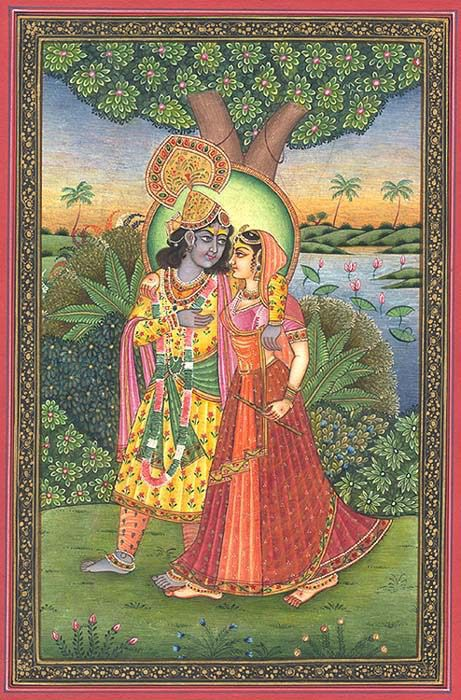
\includegraphics[width=0.8\textwidth]{pics/relationship1.png}
 \end{figure}

 

\subsubsection{1. DINA KUTA}
 

Count the Nakshatra of the man from that of the woman and divide the number by nine.
If the remainder is an even number: 0, 2, 4, 6, or 8, the result is good. If it is an odd number; 1, 3, 5, 7, 9, the result shows difficulties. Three units of compatibility are given if the result is good.
 

The idea is that the woman being feminine in nature should have a Nakshatra in a feminine (even numbered) relationship from that of the man.

 

\subsubsection{2. GANA KUTA}
 

The Nakshatras are classified into three temperaments or energy types (gana) as Deva (divine), Manusha (human) or Rakshasa (demonic). They generally correspond to sattvic, rajasic and tamasic qualities. They also have an energetic effect.

 

Deva or divine Nakshatras are characterized by faith, openness, loyalty and devotion, which however, may be conservative or superficial.
Manusha or human Nakshatras are characterized by change, turbulence and uncertainty, which however, may be progressive.
Rakshasa Nakshatras are characterized by negation, independence, eccentricity, and harsh actions, which however may lead a person to break through attachments or conventions.
 

These groups do not of themselves make the individuals born under them of higher or lower spiritual nature. That comes from the chart as a whole.

 

Generally, one should marry a person of the same Gana. It is also considered that a Rakshasa man can marry a Deva or Manusha girl, but that a Deva or Manusha man should not marry a Rakshasa girl. These Ganas are as follows:

 

DEVA GANAS are Ashvini, Mrigashira, Punarvasu, Pushya, Hasta, Svati, Anuradha, Shravana, and Revati.
MANUSHA GANAS are Bharani, Rohini, Ardra, Purva Phalguni, Uttara Phalguni, Purvashadha, Uttarashadha, Purva Bhadra, and Uttara Bhadra.
RAKSHASA GANAS are Krittika, Aslesha, Magha, Chitra, Vishakha, Jyeshta, Mula, Dhanishta and Shatabhishak.
 

This factor counts for six units. Some astrologers say that if the Nakshatra of the woman is more than 14th from the man, this problem can be ignored.

 

We also note that Deva Nakshatras are good Moons under which to proceed with any favorable actions. Manusha are moderate, and Rakshasa are usually not recommended. We can note their effects under the section of Part III on Astrological Forecasting Part 1, to see their nature and results.

 

\subsubsection{3. MAHENDRA}
 

It is good if the Nakshatra of the man is 4th, 7th, 10th, 13th, 16th, 19th, 22nd or 25th from that of the woman.

 

\subsubsection{4. STRI DIRGHA}
 

The Nakshatra of the male should be at least nine away from that of the female. By some accounts seven is enough. The idea is that some distance between the Moons is helpful for compatibility. This consideration can be ignored if Rashi Kuti (factor 6) or Graha Maitri (factor 7) prevail.

 

\subsubsection{5. YONI KUTA}
 

This is perhaps the strangest factor of compatibility in Vedic Astrology. It divides the Nakshatras into several animal types, said to represent their sexual organs. It is thought to measure sexual compatibility between the partners.

 

\subsubsection{NAKSHATRAS AND RULING ANIMALS}

\begin{center}
\begin{tabular}{ l l l l}

 NAKSHATRAS              & ANIMAL             &SEX \\

1.    ASHWINI	&HORSE	&MALE.                             \\
2.    BHARANI	&ELEPHANT	&MALE.                      \\
3.    KRITTIKA	&SHEEP	&FEMALE                           \\
4.    ROHINI	&SERPENT	&MALE                         \\
5.    MRIGASHIRAS	&SERPENT	&FEMALE                         \\
6.    ARDRA	&DOG	&FEMALE                         \\
7.    PUNARVASU	&CAT	&FEMALE                         \\
8.    PUSHYA	&SHEEP	&MALE                         \\
9.    ASHLESHA	&CAT	&MALE                         \\
10.  MAGHA	&RAT	&MALE                         \\
11.  PURVA PHALGUNI	&RAT	&FEMALE                         \\
12.  UTTARA PHALGUNI	&COW	&MALE                         \\
13.  HASTA	&BUFFALO	&FEMALE                         \\
14.  CHITRA	&TIGER	&FEMALE                         \\
15.  SWATI	&BUFFALO	&MALE                         \\
16.  VISHAKHA	&TIGER	&MALE                         \\
17.  ANURADHA	&RABBIT	&FEMALE                         \\
18.  JYESHTA	&RABBIT	&MALE                         \\
19.  MULA	&DOG	&MALE                         \\
20.  PURVASHADHA	&MONKEY	&MALE                         \\
21.  UTTARASHADHA	&MONGOOSE	&MALE                         \\
22.  SHRAVANA	&MONKEY	&FEMALE                         \\
23.  DHANISHTA	&LION	&FEMALE                         \\
24.  SHATABHISHAK	&HORSE	&FEMALE                         \\
25.  PURVA BHADRA	&LION	&MALE                         \\
26.  UTTARA BHADRA	&COW	&FEMALE                         \\
27.  REVATI	&ELEPHANT	&FEMALE                         \\
 
 \end{tabular}
\end{center}
 

\subsubsection{HOSTILE OR INCOMPATIBLE ANIMALS}

 

These are the horse and buffalo, elephant and lion, sheep and monkey, serpent and mongoose, dog and rabbit, cat and rat, cow and tiger. Combinations of these should be avoided in marriage. Generally, this is enough to reject a marriage according to this system. This gives 0 points in terms of Yoni Kuta.

 

\subsubsubsection{UNFRIENDLY ANIMALS}

HORSE	cow, tiger, lion	ELEPHANT	tiger
SHEEP	dog, rat, tiger, lion	SERPENT	cat, rat, cow, buffalo
DOG	sheep, rat, tiger, mongoose, lion	CAT	serpent, tiger, mongoose, lion
RAT	sheep, serpent, dog, mongoose	COW	horse, serpent, lion
BUFFALO	Serpent, tiger, lion	TIGER	horse, elephant, sheep, dog, cat, buffalo, rabbit, monkey, lion
RABBIT	Horse, tiger, lion	MONKEY	tiger
MONGOOSE	Dog, rat	LION	horse, sheep, dog, cat, cow, tiger, rabbit.
 

These are counted from the Nakshatra of the male. Marriage between unfriendly animals is considered to be more difficult. They give 1 point in terms of Yoni Kuta.

 

\subsubsubsection{NEUTRAL ANIMALS}

HORSE	Elephant, sheep, dog, cat, mongoose	ELEPHANT	sheep, serpent, buffalo, monkey
SHEEP	Elephant, cow, buffalo, mongoose	SERPENT	horse, elephant
DOG	Horse, elephant, serpent, cat, cow, buffalo, monkey	CAT	horse, elephant, sheep, dog, cow, buffalo, mongoose
RAT	Horse, elephant, cow, buffalo, tiger, rabbit, monkey, lion	COW	elephant, dog, cat, rat, monkey, mongoose
BUFFALO	Dog, cat, rat, rabbit, monkey, mongoose	TIGER	serpent, rat, mongoose
RABBIT	Elephant, sheep, serpent, rat, buffalo, monkey, mongoose	MONKEY	serpent, dog, rat, cow, buffalo, rabbit, lion
MONGOOSE	Horse, elephant, cat, cow, buffalo, tiger, rabbit, lion	LION	serpent, rat, buffalo, monkey, mongoose
 

These are considered average in terms of compatibility. They give 2 points in terms of Yoni Kuta.

 

\subsubsubsection{FRIENDLY ANIMALS}

HORSE	serpent, rabbit and monkey	ELEPHANT	sheep, serpent, buffalo and monkey
SHEEP	elephant, cow, buffalo and mongoose	SERPENT	horse, elephant
DOG	None	CAT	rabbit, monkey
RAT	None	COW	sheep, buffalo, rabbit
BUFFALO	elephant, sheep, cow	TIGER	none
RABBIT	cat, cow	MONKEY	horse, elephant, cat, mongoose
MONGOOSE	sheep, monkey	LION,	none
 

These relationships are also determined from the Nakshatra of the male. Hence, a man under the horse will generally do well with a woman under the serpent, as there is friendship between their animals. These give 3 points in terms of Yoni Kuta.

 

\subsubsubsection{SAME ANIMAL}

 

Marriage between men and women of the same animal is considered to be the best, particularly if they are of male and female stars respectively, for example, an Ashwini man and a Shatabhishak woman. It is conducive to sexual compatibility and happiness through children. Relationships of the same animal give 4 points in terms of Yoni Kuta.

 

Some animal types are difficult in terms of sexual compatibility. Such are, in order of difficulty, the tiger, lion, dog and rat, which have no friendly animals. Those of these animal types have more difficulty in sexual relationships. The serpent, cat and rabbit have some difficulties as well. Most generally compatible are the monkey and elephant. The others fall in the middle.

 

In addition, it is more favorable if the males animal falls in a masculine division and if the womans animal falls in a feminine division. Please note the table at the end of this lesson, which allows you to look up the compatibility numbers between various Nakshatras based upon this principle.

 
\begin{figure}[H]
 \centering
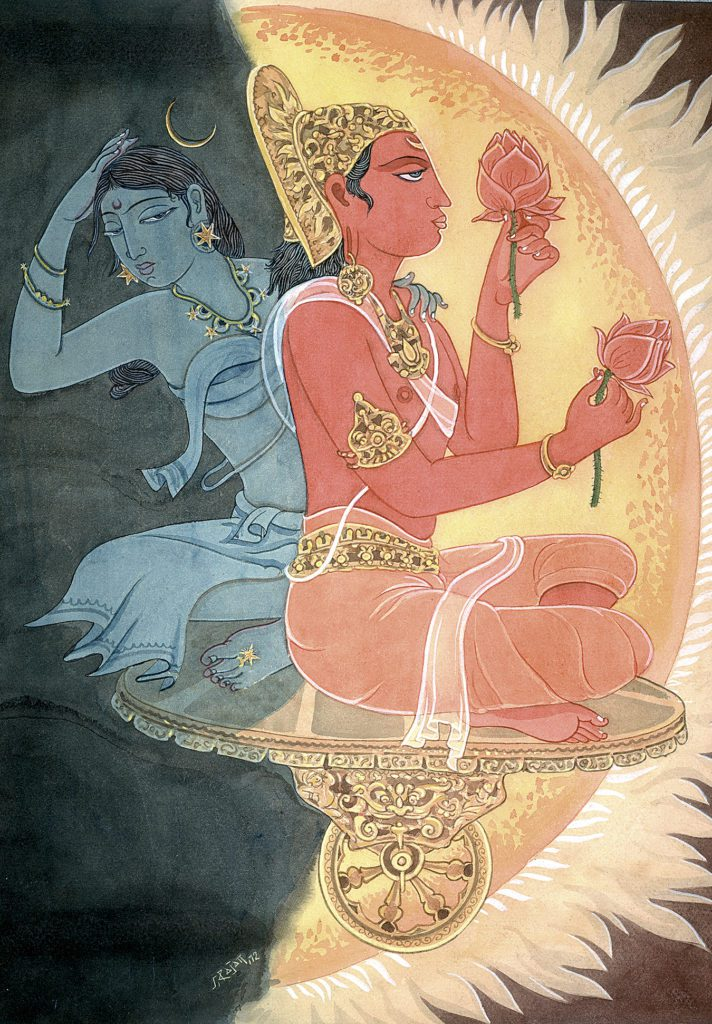
\includegraphics[width=0.8\textwidth]{pics/relationship2.png}
\caption{Lord Shiva and Parvati Devi}
 \end{figure}




\subsubsection{6. RASHI KUTA}
 

This refers to the relationship between the Moon signs (Chandra Rashis) in the birthchart, which is obviously an important consideration in all astrological compatibility examinations. Vedic Astrology gives us a system to compute this relationship.

 

If the Moon sign of the male is SECOND from the female, and hers is twelfth from his, it is not considered good. For example, if the male has the Moon in Virgo and the female has it in Leo. On the other hand, if the males Moon is twelfth from the female, it is considered good, ie. if his is in Leo and hers is in Virgo.

 

If the Moon sign of the male is THIRD from the female, this gives difficulty and sorrow, but if the Moon sign of the female is third from the male, this gives ease and happiness.
If the Moon sign of the male is FOURTH from the female, this is said to give poverty, but if the Moon sign of the female is fourth from the male, this is said to give wealth.
If the Moon sign of the male is FIFTH from the female, this is said to give unhappiness, while if her Moon sign is fifth from his it is said to give joy.
If his Moon sign is SIXTH from hers it causes difficulty to children but if hers is sixth from his, it gives happiness through children.
If the Moon signs are SEVENTH or opposite each other this is best. It gives mutual health and happiness. Moons opposite each other give balance and capacity for communication.
 

The general logic of this sequence is that it is better for the mans Moon to be placed before the womans Moon in the zodiac. As planets cast their aspects forwards in the zodiac, this gives the males chart the lead in action, which is in harmony with the nature of masculine energy. If the females Nakshatra is before in the zodiac, this can make her dominant over him.

 

If the Moon sign is the same for both partners, the Nakshatra in which the Moon is located should be different. That of the male should be before that of the female. For example, if both have Aries Moons, it is better if the mans Moon is in Ashwini, which is in early Aries, and the womans is in Bharani, which is in later Aries. However, in the actual total Kuta system, the same Moon sign is generally good whether the Nakshatra of the male is before or after that of the female.
If the Nakshatra is also the same for both partners this is considered GOOD in the case of Rohini, Ardra, Magha, Hasta, Vishakha, Shravana, Uttara Bhadra, and Revati.
It is considered AVERAGE if the Nakshatras are Ashvini, Krittika, Mrigashiras, Punarvasu, Pushya, Purva Phalguni, Uttara Phalguni, Chitra, Anuradha, Purvashadha and Uttarashadha.
It is considered NOT GOOD and not recommended in the case of Bharani, Ashlesha, Svati, Jyeshta, Mula, Dhanishta, Shatabhishak and Purva Bhadra.
 

Some astrologers consider that it is all right if the birth Nakshatra is the same if the Moons are located in different quarters within the Nakshatra. In regard to Shatabhishak, Hasta, Swati, Ashwini, Krittika, Purvashadha, Mrigashiras and Magha, it is considered all right if both partners are born in the first quarter of the Nakshatra.

 

This factor has 7 units and so is weighted fairly strongly. However, we might want to consider it in more detail. What is being weighed is the relationship between the Moon signs or the Moon to Moon relationship. For this, we can go back to the first section on Relationship and examine the relationship between Moons in the chart as a whole.

 

\subsubsection{7. GRAHA MAITRAM}
 

This refers to the relationship between the lords of the Moon signs in terms of friendship or enmity. Some astrologers count this only in terms of natural friendship, others consider the temporal as well. I am inclined to the latter opinion.

 

For example, if the mans Moon is in Pisces ruled by Jupiter and the womans Moon is in Aries ruled by Mars, then their Moon lords are natural friends.

 

When the planets involved are both friends, this factor is obtained in full. When one is a friend and the other is neutral, it is still good. When both are neutral it is only average or passable. When one is neutral and the other is inimical, it is difficult. When both are enemies, this factor of compatibility does not exist.

 

When this factor is not present in the Moons sign, it is sometimes looked for in the Moons Navamsha. This factor counts for 5 units. To determine this, we have to look at each chart separately.

 

\subsubsection{8. VASHYA KUTA}
 

The Moon sign gains power to influence or control other signs, which is referred to here. These are for:

 

Aries – Leo and Scorpio.
Taurus – Cancer and Libra.
Gemini – Virgo.
Cancer – Scorpio and Sagittarius
Leo – Libra
Virgo – Pisces and Gemini
Libra – Capricorn and Virgo
Scorpio – Cancer
Sagittarius – Pisces
Capricorn – Aries and Aquarius
Aquarius – Aries
Pisces – Capricorn
 

We see that a few signs are mutually influencing. These are Gemini and Virgo, Cancer and Scorpio. This factor counts for two kuta points.

 

\subsubsection{9. RAJJU KUTA}
 

Rajju means rope. It shows possibilities of misfortune in married life. The Nakshatras are divided into five groups based upon this factor. This factor counts for four points.

 

FOOT– Padarajju
Ashvini, Ashlesha, Magha, Jyeshta, Mula, Revati
HIP– Katirajju
Bharani, Pushya, Purva Phalguni, Anuradha, Purvashadha, Uttara Bhadra
NAVEL– Udararajju
Krittika, Punarvasu, Uttara Phalguni, Vishakha, Uttarashadha, Purva Bhadra
THROAT– Kantharajju
Rohini, Ardra, Hasta, Swati, Shravana, Shatabhishak
HEAD – Shirorajju
Dhanishta, Chitra, Mrigashira
 

The Nakshatras wherein the Moon is located should not fall in the same Rajju for male and female. If they both occur in the head, the husbands longevity may be threatened. If they both occur in the throat, the wifes longevity may be threatened. If they both occur in the stomach, the childrens longevity may be threatened. If they both occur in the navel, there may be poverty. If they both occur in the hip, the couple may have to always be wandering.

 

\subsubsection{10. VEDHA/ INCOMPATIBLE NAKSHATRAS}
 

Each Nakshatra has one that it particularly afflicts and with which it is therefore generally incompatible. It is best for those of these conflicting Nakshatras not to marry each other. This factor counts for two points. These are:

 

1. Ashwini and 18. Jyeshta	2. Bharani and 17. Anuradha
3. Krittika and 16. Vishakha	4. Rohini and 15. Swati
5. Mrigashira and 23. Dhanishta	6. Ardra and 22. Shravana
7. Punarvasu and 21. Uttarashadha	8. Pushya and 20. Purvashadha
9. Ashlesha and 19. Mula	10. Magha and 27. Revati
11. Purva Phalguni and 26. Uttara Bhadra	12. Uttara Phalguni and 25. Purva Bhadra
13. Hasta and 24. Shatabhishak.	14. Chitra, no incompatible Nakshatras
 

 

\subsubsection{11. VARNA/ CLASS}
 

The lunar signs are divided into four groups based upon class or varna. Brahmin is the spiritual class or those of knowledge, Kshatriya the nobility or people of honor, Vaishya the merchants or commercial people, and Shudra, the servant or labor class. They tend to represent our temperament and values, but are only very vague indications of these that should not be taken too seriously. These are:

 

 BRAHMIN	 water signs	 Cancer, Scorpio, Pisces
 KSHATRIYA	 fire signs	 Aries, Leo, Sagittarius
 VAISHYA	 air signs	  Gemini, Libra, Aquarius
 SHUDRA	 earth signs	 Taurus, Virgo, Capricorn
 

The unit of agreement here is only 1 point. This we might add, however, is an extremely important factor to consider, namely spiritual compatibility. However, the method of calculating it here is very approximate and rarely accurate. It is better to use other more complex and accurate methods of judging spiritual types.

 

\subsubsection{12. NADI KUTA}
 

This is an attempt to compute the physical type according to the three Ayurvedic doshas. By this system, individuals of the same doshic type should not marry, as they will increase the factors of disease in each other. Each of the Nakshatras is assigned one of them.

 

VATA
Ashvini, Ardra, Punarvasu, Uttara Phalguni, Hasta, Jyeshta, Mula, Shatabhishak, Purva Bhadra
PITTA
Bharani, Mrigashiras, Pushya, Purva Phalguni, Chitra, Anuradha, Purvashadha, Dhanishta, Uttara Bhadra
KAPHA
Krittika, Rohini, Ashlesha, Magha, Swati, Vishakha, Uttarashadha, Shravana, Revati
 

If Nadi Kuta is not present, it can be counted on the quarters of the Nakshatras. If it is present there, that can also be helpful. This factor is given 8 units. However, we should note that it is only approximate. The Nakshatra in itself is not always enough to determine constitutional type. Hence, if we have another way of determining it, we should resort to that instead.

 

\subsubsection{SUMMARY}

 

In summary, we note that the factors examined in this system are important but the way in which some of them are gauged is not beyond question. Perhaps this system may have to be revised relative to modern conditions. However, it is still very helpful and all Vedic astrologers should know how to use it, particularly if they will be dealing with Indian clients.

 

Please look up the Kuta or chart compatibility on your Vedic software system.  Compare the star or Nakshatra of the male partner (bridegroom) with the female partner (bride). This gives a general compatibility rating considering most of the points of the computative method.

 

Good compatibility is usually above 20 points, though as little as 18 can be all right and is average. High compatibility is above 25 points. Low compatibility is below 15 points. Below 10 can be very difficult.

 

While in India this method is taken very seriously, here I dont think we can follow it rigidly. I have seen at least some successful or enduring marriages with less than 15 points of compatibility. I have also seen some divorces with more than 25 points. It is obvious that based on Nakshatra alone there will be many people that we will be compatible with in terms of this method alone.

 

\subsubsection{MEANING OF THE KUTA SYSTEM}

 

This system measures primarily the compatibility between the Moons and Nakshatras. This is very important because the Moon shows emotional affinity and the ability to function together as a family. However, a good Moon relationship is not enough for a successful relationship. And relationships can be successful without good Moon relationships if Venus and Jupiter are favorably placed between the charts.

 

When the Moons are favorable, we feel good around one another, our moods harmonize, and we do not feel invaded or threatened by the other persons presence in our lives. When the Moons are unfavorable, it may be difficult to trust the other person, or to feel that we can be ourselves around them. They are much more likely to seem foreign, alien or different from us.

 

Therefore, it is best to use the computative method along with the comparative method, considering the overall nature of the charts involved. By itself the Kuta system can cause us to make hasty or superficial judgments. Usually if the points are high, that is good, if the charts are otherwise in harmony. If the points are low, that can be counteracted (unless the total points is very low, like below 10) if the charts are otherwise in harmony. If the points are high and the charts are otherwise disharmonious, it will not be sufficient for a good relationship. If the points are low but the charts are otherwise harmonious, it may be sufficient for a good relationship.

 

Generally speaking, there is little that can counteract the effects of a bad seventh house in the chart, while there is little that can damage a good seventh house in the chart. Please remember this point.

 

We should first examine the computative method, as it is quick to note, and then go into comparative analysis for a more clear decision on the matter.
We have also included for easy computation, a chart of the Yoni Kuta.
 



 

\subsubsection{ASTROLOGY AND RELATIONSHIP COUNSELING}

 

Astrology is a helpful tool in relationship counseling because it reveals the energetic issues behind relationships. It can help each person see their partners view of the world, which is usually not the same as their own. It can also help show the factors of projection – what we are imagining about the partner – which may not be their nature and must eventually cause problems. Sometimes we may be relating to one planetary influence in another person but not the others.

 

Yet relationship counseling can be difficult, particularly for clients having trouble in their relationships with each other, for those seeking divorce, or if one partner is trying to use the reading to get the other partner into or out of a marriage. For this reason, we recommend doing individual readings before doing readings for couples. It is easiest to do a compatibility reading if the relationship is just beginning and no major commitments and attachments have been formed. If the relationship is already established, we might want to orient the reading more toward helping the couple understand each other, rather than telling them if they are really compatible in the long run. Hence, a certain amount of discretion may be required, even the charts do not look good together.

 

This is the easiest area of astrological counseling where we can offend or upset other people, even if we are right. The important thing is to give the client advice that they are able to use.

 

These relationship issues have been mainly oriented toward male-female or marriage relationships. However, they apply to some extent to all human relationships. People with whom we have disharmonious Moons are likely to be trouble to work with or be friends with. Other relationship incompatibilities, whether judged by the comparative or computative methods, can yield similar problems. Hence, if we have an associate that it is particularly easy or particularly difficult to be with, it can help to examine the charts to see what the conflicting patterns may be.

 

Even as astrologers we can be aware of these patterns. For example, I have Mars in Scorpio in my birthchart. Hence I understand that clients with the Moon in Scorpion are more likely to feel criticized, hurt or even offended by what I may say because of the effect of Mars on the Moon. With them I am inclined to be particularly sensitive to avoid hurting their feelings even on minor issues.
\newpage

\section{SHADBALA: THE SIX MEANS OF DETERMINING PLANETARY STRENGTHS AND WEAKNESSES}
 

In this lesson, we will examine the most complex system found in Vedic, or for that matter, any system of astrology for determining the power of the planets in the chart. This information is largely for reference and need not be understood in detail, particularly in regard to calculation which is offered by Vedic astrology software and can be quite complex.

 

Most astrologers like to calculate. Many would like a system of calculations that would guarantee the rightness of all their predictions. All that we would have to do would be to run a program and we would know the strength and weakness of planets and exactly what they will do in each chart. However, life is very complicated. The influence of the planets can come on several different levels and we have some freedom as to how we use these influences. Hence, all such mechanical systems should be applied with discretion. They are a good place to start but cannot be relied on entirely. The information below is mainly for reference value.

 



 

Shadbala is an elaborate system of computations to aid in determining planetary strengths and weaknesses. It is perhaps the most sophisticated and detailed of all such astrological systems. It requires much astronomical knowledge to compute accurately. While Shadbala is not necessary to give an accurate astrological reading, it is helpful information to have. As the calculations are very complex and would require much skill and time to do oneself, various computer programs are preferable.

\subsection{\textbf{Audio Overview by Dr. David Frawley on Shadbala}}

Once computed, all the different types of Shadbala are averaged out to determine the general planetary strength or weakness. Generally, it is considered that if a planet has a Shadbala of 1.0 or more it has the power to give the effects of its position in the chart. If its Shadbala is less than 1, it is considered weak and may cause difficulty. Shadbalas occur commonly up to 1.3 and uncommonly as high as 1.8. They occur commonly as low as .8 and uncommonly as low as .6. They average around 1.1 or 1.2.

 

Some astrologers, however, consider only the Rupa total on the Shadbala. In this way, they like to discover what is the strongest and what is the weakest planet in the chart in terms of Shadbala prior to any special divisions of the amount.
Other astrologers look more at the particular factors in Shadbala, like exaltation strength (uccha bala) and are not so concerned about the total figures for the planet.
 

I am more of the second opinion. Shadbala is not absolute. If a planet has a high Shadbala, it does not necessarily mean it will always give good results or if it has a low one, it does not mean that it will give bad results. Other factors have to be taken into consideration (see Ishta and Kashta Phala, Good and Bad Results of Planets). Similarly, if a planet has only average Shadbala but is strong in the chart in terms of position and aspect, it can still act in a very potent manner. Shadbala shows the basic strength and weakness of planets but we have to look back to the chart for what they are empowered to do.

 

Shadbala does not appear to adequately consider planetary aspects. It does read aspectual strength into its factors but this does not count for much. It seldom makes a difference of more than 5%. My experience has been that aspects are probably more important than any Shadbala factors.

 

I have given additional criticism to Shadbala as its factors sometimes cancel each other out. While its calculations are each useful to consider in themselves, it is not always useful to average them all out. Astrology requires qualitative judgments and these cannot always be reduced to mere quantitative calculations. There is still no substitute for insight and experience.

 

While all the factors of Shadbala are important and should be considered to some degree (like whether a planet is strong by location, position or aspect), the present system of Shadbala for doing this may not be entirely accurate. I would like to see Shadbala researched and revamped into a more workable system. Hence, I have presented this material primarily for reference, regarding the individual factors as more important than their overall average. These calculations provide us much information about how to view the planets. Otherwise a simple examination of the chart relative to usual factors of sign, house, aspect and yoga is much more important.

 

\subsection{MAIN FACTORS OF SHADBALA}

 

The six factors of Shadbala are:

\begin{enumerate}
\item[*] Positional Strength (Sthana Bala)
\item[*] Directional Strength (Dig Bala)
\item[*] Temporal Strength (Kala Bala)
\item[*] Motional Strength (Chesta Bala)
\item[*] Natural Strength (Naisargika Bala)
\item[*] Aspectual Strength (Drik Bala)
\end{enumerate} 

 


\subsection{1. POSITIONAL STRENGTH}
This consists of five factors:

 

\begin{enumerate}
\item[*] Exaltation Strength (Ucha Bala)
\item[*] Divisional Strength (Saptavargaja Bala)
\item[*] Odd-Even Sign Strength (Ojayugmarasyamsa Bala)
\item[*] Angular Strength (Kendra Bala)
\item[*] Decanate Strength (Drekkana Bala)
\end{enumerate} 

\subsubsection{A. EXALTATION STRENGTH}


 

Exaltation Strength is always important and should be considered even when Shadbala is not calculated. Planets are always stronger at exaltation and weakest at their fall. This is similar to the Moon being stronger full than when new. The determination of Exaltation Strength is simple.

A planet is given 60 points of value when at the degree of exaltation and 0 points of value when at the degree of fall.
For every three degrees away from exaltation, it loses one point and for every three degrees away from fall it increases one point.
 

Exaltation Strength does have its limitations. First, it does not consider how much the fall of a planet may be canceled (and if the fall can be canceled, the exaltation should be canceled by opposite factors). Second, it does not consider the sign location of planets. Planets do not lose their strength in a uniform manner between exaltation and fall, as they gain strength in the signs they rule.

 

For example, the Sun in Leo has a low exaltation strength as it is nearer to its fall in Libra than its exaltation in Aries, but it is still strong being in its own sign. In my consideration of planets I like to consider both exaltation and sign residency strength together. If we consider them separately, as Shadbala does, they may cancel each other out. For example, the Sun though strong by residency in Leo is weak by exaltation strength, hence neutral. However, I think it should still be generally considered as strong as its position in its own house cancels the weakness in exaltation strength.

 

\subsubsection{B. DIVISIONAL STRENGTH}

 

This is calculated relative to the seven divisional charts of the divisional first, second, third, seventh, ninth, twelfth and thirtieth charts. It follows the same rules of friendship and enmity as that of the birthchart, giving each a certain point total.

 

Divisional Strength of Planets

\begin{center}
\begin{tabular}{ l l l l}
Own sign	& 30 points.                 \\
Great friend	 &22.5 points                \\
Friend	 &15 points                \\
Neutral sign	 &7.5 points                \\
Inimical sign	 &3.75 points                \\
Great enemy	 &1.875 points                \\
\end{tabular}
\end{center}
 

It is necessary to determine the planetary friendships and enmities for all seven divisional charts to do this. There is the special consideration that a planet in its Mulatrikona division in the basic birth or divisional first (rashi) chart would get 45 points. Otherwise, Mulatrikona is not considered.

 

This is an important consideration generally speaking and is always worthy of noting by itself.

 

\subsubsection{C. ODD OR EVEN SIGN STRENGTH}

 

Planets gain strength whether in odd or even signs in the Rashi (divisional first) and Navamsha (divisional ninth).

Sun, Mars, Jupiter, Mercury and Saturn do better in odd-numbered signs
Moon and Venus do better in even-numbered signs
 

Hence, most planets gain strength in odd signs and lose it in even signs.

 

Planets get 15 points for being in their appropriate odd or even sign in both the Rashi and Navamsha, giving them a maximum of 30 points in this regard. This is a minor point and it is not given a lot of weight. However, it can be canceled by other factors. Mercury, for example, has no odd and even strength by sign in Virgo, though exalted.

 

\subsubsection{D. ANGULAR STRENGTH}

 
\begin{center}
\begin{tabular}{ l l l l}
Planets in angular houses	 &60 points               \\
Planets in succedent houses	& 30 points               \\
Planets those in cadent houses	 &15 points               \\
 \end{tabular}
\end{center}

This is an important factor because planets are usually stronger in angles. House qualities are important factors in all delineations and must always be considered even if we are not figuring Shadbala.

 

Yet this naturally depends upon the house system we use. If we use a midheaven system like the Placidian or Indian Sripati system, we will get different results than using the equal house systems. But even though some computer programs for Vedic Astrology allow for different house systems, they may calculate the Shadbala only by the house-sign system (the system of house formation that judges houses by sign only).

 

This type of strength has two limitations. First, it does not consider the meaning of the houses adequately. For example, the ninth, though a cadent house, is still good by its being the best trine, and is an excellent position for most planets, particularly benefics. We could not consider Jupiter to be weak here though it would suffer by angular strength according to Shadbala. Second, it may be canceled somewhat by directional strength. For example, the Moon though in an angle in the tenth house, suffers from being in its weakest place (the south) in terms of direction.

 

Another problem is that malefics in angles can be strong to do evil and may harm the person. Saturn in the Ascendant where it has angular strength may harm the person or render them them weak.

 

\subsubsection{E. DECANATE STRENGTH}

Planets are divided into masculine, feminine and neuter.

 
\begin{center}
\begin{tabular}{ l l l l}
Masculine planets	 &Sun, Mars and Jupiter               \\            
Feminine planets	& Moon and Venus               \\
Neuter planets	 &Mercury and Saturn               \\
  \end{tabular}
\end{center}

They gain strength if located in the appropriate decanate or ten degree division of a sign. The rule of determining Decanate Strength is as follows:

\begin{center}
\begin{tabular}{ l l l l}
Masculine planets gain &15 points if they are located in the first decanate of a sign &(00 00—09 60).               \\
Neutral planets gain &15 points if located in the second decanate of a sign    &(10 00—19 60).               \\
Feminine planets &gain strength if located in the third decanate of a sign       &(20 00—29 60).               \\
  \end{tabular}
\end{center}

This is a minor consideration that does not count for more than 15 points. Yet it is part of a greater consideration of Decanate position in the chart. I always look at the Decanate of the Ascendant for determining its results. For example, the Gemini decanate or final ten degrees of a Libra Ascendant will have better intellectual skills as it is in a Decanate of Mercury.

 

\subsubsection{SUMMARY OF POSITIONAL STRENGTH}

 

Divisional Strength is  important and Shadbala is a significant means of determining it. I believe it is the most important part of Shadbala and that it carries most weight in the system. But it remains a general determination. It does not outweigh regular positional issues of planets by sign, house and aspect.

 

\subsection{2. DIRECTIONAL STRENGTH}
 

Directional strength (Dig Bala) is always important and should be considered even if one is not looking at the overall Shadbala.

The  idea behind Directional Strength is similar to that of Exaltation Strength. Just as planets have one sign position in which they are exalted, they have one house position in which they gain Directional Strength. The calculation is the same.

 

A planet gets 60 points of strength at the place of full Directional Strength and 0 points at the place opposite it. The intermediate positions are also divided by three. Each three degrees away from the place of Directional Strength causes a loss of one point of strength.

Planets have Directional Strength in different directions.

Directional Strength

\begin{center}
\begin{tabular}{ l l l l}
Sun and Mars	  &South (tenth house)            \\
Saturn	  &West (seventh house)            \\
Moon and Venus	 & North (fourth house)            \\
Jupiter and Mercury	  &East (first house)            \\
  \end{tabular}
\end{center}

This calculation has the same limitation as that of Angular Strength. It depends upon the house system used. Midheaven house systems will give different results than regular sign-based house systems. I prefer that.

 


\subsubsection{3. TEMPORAL STRENGTH}
 

This is a combination of nine factors based upon the time of birth in hours, days, months, years, etc.   These are:

 

\begin{enumerate}
\item[*] Day-Night Strength (Nathonnatha Bala)
\item[*] Monthly Strength (Paksha Bala)
\item[*] Four Hour Strength (Tribanga Bala)
\item[*] Lord of the Year Strength (Abdadhipati Bala)
\item[*] Lord of the Month Strength (Masadhipati Bala)
\item[*] Lord the Day Strength (Varadhipati Bala)
\item[*] Lord of the Hour Strength (Hora Bala)
\item[*] Declinational Strength (Ayana Bala)
\item[*] Planetary War Strength (Yuddha Bala)
 \end{enumerate}

This is an important factor seldom considered in Western Astrology. After Positional Strength, it is the most significant factor in Shadbala and counts for a great deal in its computation. It is a helpful general consideration, expanding the Panchanga or daily calendar considerations that we look at in Part III of the course.

 

\subsubsubsection{A) DAY-NIGHT STRENGTH}

 

There are several rules in this computation. Planets are powerful at different times of the day:

 
\begin{center}
\begin{tabular}{ l l l l}
Moon, Mars and Saturn	 & Midnight           \\
Sun, Jupiter and Venus	  &Noon           \\
Mercury is always strong	  &Always gets 60 points           \\
   \end{tabular}
\end{center}

At these times of strength, each planet gets 60 points. The amount of time that has elapsed from these times of strength is divided into sixty portions or about 24 minutes. Hence, every 24 minutes away from these times a planet loses one point in strength.

 

This is a factor of some significance but perhaps of not as much as it is given.

 

\subsubsubsection{B) MONTHLY STRENGTH}

 

This computation similarly has its rules. Planets are stronger during certain times of the lunar month:

 

\begin{enumerate}
\item[*] Benefics – bright lunar fortnight or waxing Moon
\item[*] Malefics – dark lunar fortnight or waning Moon
 \end{enumerate}

Benefics are Jupiter, Venus, the Moon when bright and an unafflicted Mercury. Malefics are the Sun, Mars, Saturn, the Moon when not bright and an afflicted Mercury.

 

The factors of calculation are as follows:

\begin{enumerate}
\item[*] The distance of the Moon from its position when new is divided by three. This amount is added to benefic planets.
\item[*] The distance the Moon from its position when full is divided by three and this is added to malefics. Sixty is thus the maximum.
  \end{enumerate}

On the other hand, if the Moon is near new or considered malefic, the calculation is reversed.

\begin{enumerate}
\item[*] The distance the Moon from its position when new is divided by three. This amount is added to malefic planets.
\item[*] The distance the Moon from its position when full is divided by three and this is added to benefics.
  \end{enumerate}

The amount ascribed to the Moon is sometimes doubled.

 

\subsubsubsection{C) FOUR HOUR STRENGTH}

 

Here we divide both day and night into three equal portions or about four hours each. It will vary by the season as the Hindu day is counted from sunrise. It is a secondary consideration.

The planet that rules this period, approximately four-hours, a third portion of day or night, gets 60 points of strength.

 

Mercury	  first third of the day	Sun	  middle third of the day
Saturn	  final third at the end	Moon	  first third of the night
Venus	  middle of the night	Mars	  final third of night
Jupiter	  always gets 60 points		always strong
 

This factor is similar to Day-Night Strength and can cancel it out. For example, Mars is most powerful at midnight in Day-Night Strength but in terms of Four Hour Strength, it is most powerful a couple of hours before sunrise.

 

\subsubsubsection{D-G) LORD OF THE YEAR, MONTH, DAY AND HOUR STRENGTH}

 

The rules here are very simple:

 

Lord of the year	 15 points	Lord of the month	 30 points
Lord of the day	 45 points	Lord of the hour	 60 points
 

These calculations are more complex than they appear. The year is considered to be of 360 days and it is counted off from the theoretical beginning of creation some more than 714,000,000,000 years ago! The Lord of the Month is the planet that rules the weekday of the month during which the birth occurs. This is by a 30-day month from the same theoretical creation eons ago.

 

The Lord of the Day is the planet ruling the day in the normal sequence Sun-Sunday, Moon-Monday, Mars-Tuesday etc., with the normal Hindu day counted from sunrise to sunrise. (Though this turns out the same if it is calculated from the mythic beginning of creation). The Lord of the Hour is according to the planets ruling the hour starting daily from sunrise (see Planetary Hours).

 

Generally a person will do better when under the influence of the hour, day, month and year lords as found at birth. When these repeat themselves during the course of a persons life great changes occur.

 

\subsubsubsection{H) DECLINATIONAL STRENGTH}

 

This strength considers the declinations of planets (how far north or south of the zodiacal equator that they are). We could also refer to it as “Equinoctial or Seasonal Strength”. It is similar to and has the same weight as Angular and Directional Strength.

 

First we have to convert from the Sidereal to the Tropical Zodiac to arrive at the directional points of the solstices and equinoxes. This we can do by adding our Ayanamsha to the position of the planets. On this some other complex calculations are added. The rule is: A planet with the best Directional Strength gets 60 points, down to 0 at the worst, losing one point every three degrees away from their maximum point of directional strength.

 

We must then consider the specific points of Declinational Strength for each planet, which varies relative to (but not exactly the same as) their position via the solstice and equinoctial points:

 

Sun, Mars, Jupiter and Venus	 place of summer solstice
Moon and Saturn	 place of winter solstice
Mercury	 place of the equinoxes
 

Sun, Mars, Jupiter and Venus do best when their declination is at the furthest point north, while the Moon and Saturn do better when it is at the furthest point south. Mercury does best when it is at the equatorial or neutral point, neither north nor south.

 

Hence we can ascertain Declinational Strength generally by noting the declinations of the planets, or by seeing how close to the solstice points they may be.

 

\subsubsubsection{I) PLANETARY WAR STRENGTH}

 

This is a special factor that only comes into play when planets (not including the Sun and Moon) are located within one degree of each other. As per the rules of planetary war, the planet with the lower position in degrees and minutes wins. By other accounts, the planet with the higher declination (further north relative to the ecliptic) wins. Points are added to the victor and subtracted from the loser according to the amount of strength of the planet generally and the relative size of its disc.

 

Planets can gain or lose significantly by planetary war, but the nature of the planets also comes into play here. Venus would lose more in a Planetary War with Mars than with Mercury, as it is generally an enemy of Mars but a friend of Mercury.

 

Generally, I don’t rate planetary war very highly by itself but look more at the nature of the conjunction by the natural and temporal statuses of the planets involved.

 

\subsubsubsection{SUMMARY OF TEMPORAL STRENGTH}

 

While important, it still has limitations. It is good to consider if a planet has some factor of Temporal Strength to give it power. Such factors are whether birth has taken place at a favorable time during the day, month or year for the planet or during a day, month or year ruled by the planet.

 

\subsubsection{4. MOTIONAL STRENGTH}
 

By one system, this is said to consider the distance of a planet from the Sun. Planets are strongest when furthest away from the Sun and weakest when in conjunction with it. They get 60 points when at the furthest point away and 0 when in conjunction with it. As Mercury and Venus never get far from the Sun, their position is not as easy to determine.

 

Yet the calculations to do this are more complicated than that. Motional strength for the Sun and Moon is figured as well, but this is related to Ishta and Kashta Phala, Good and Bad Results of Planets and I have not explained it here.

 


\subsubsection{5. NATURAL STRENGTH}
 

This is the same in all charts and has its own intrinsic value that we must look at in all charts under all circumstances. It mainly reflects the brightness of planets as seen from the Earth. The planets in order of strength are: The Sun, Moon, Venus, Jupiter, Mercury, Mars, and Saturn. This is in terms of apparent brightness. The Sun gets 60 points. This amount is reduced by one-seventh for the other planets in order of their brightness.

 

Sun	60 points	Moon	51 points
Venus	43 points	Jupiter	34 points
Mercury	26 points	Mars	17 points
Saturn	9 points		
 

\subsubsection{6. ASPECTUAL STRENGTH}
 

This is complicated as it considers major and minor aspects according to the exact arc and degree of aspect. Aspects of benefics are counted as positive, those of malefics as negative. The special aspects of planets are given additional weight.

 

Yet this actor seldom has little numerical value, counting from 30 points positively or negatively! It becomes one of the least important of the Shadbalas, on par with Decanate Strength.

 

This can be different than the usual strength of planetary aspects given in general chart readings in Vedic Astrology. Hence, when considering aspectual strength as part of Shadbala, we must still consider aspects in the chart itself as having their own weight apart from Shadbala. The power of aspects in the chart is not limited to it.

 

 

\subsubsection{TOTAL SHADBALA}

 

All the factors of Shadbala are added together. This total is called “Virupa”. This is divided by 60 and becomes the “Rupa” total. I like to examine this and note particularly which planet is strongest and which planet is weakest. It is this Shadbala calculation that is given the most weight.

 

This amount is divided differently relative to each planet:

Division of Rupa Total by Planet

Sun                by 5 or 6

Moon              by 6

Mars               by 5

Mercury          by 7

Jupiter            by 6.5

Venus            by 5.5

Saturn            by 5

 

This gives the Shadbala Power Ratio. A planet requires a power ratio of at least 1.0 to have sufficient Shadbala strength. Most planets get this rather easily. Saturn is most likely to be low. Planets with higher Shadbalas gain greater power and over those with lower. This is usually the case.

 

However, I have seen charts with all planets high in Shadbala and the person has had a miserable life and accomplished nothing. This can be traced to common afflictions like bad aspects or difficult house positions. These things cannot simply be erased by positive Shadbala indications.

 

I have also seen people with charts that have no planets high in Shadbala doing quite well. I have seen genius Mercury types with an average Mercury Shadbala. On the other hand, I have seen several instances of weak hearts with a low Shadbala for the Sun. Yet, generally if a Shadbala is either very low or very high, it will indicate something very weak or very strong about the planet. Average Shadbalas may give good or bad results depending upon other factors.

 

Therefore, though of general value, the details of Shadbala may require a specific analysis for us to really benefit from them. 

 

\subsubsection{GOOD AND BAD RESULTS OF PLANETS (Ishta and Kashta Phala)}
 

Called Ishta and Kashta Phala in Sanskrit, this refers to the ability of planets to give good or bad results during their periods.

 

A planets power to good during its period is determined by multiplying its Exaltation Strength by its Motional Strength and taking the square root of it. Its power to do ill is determined by subtracting the Exaltation Strength by sixty and the Motional Strength by 60, multiplying them and taking the square root of that. These two totals are compared. If the power to do good is higher, then the planet will give good results during its periods. If the power to do ill is higher, it will tend to cause difficulties.

 

Such elaborate calculations seldom counter the obvious indications in a chart and so mainly relate to more detailed research or fine-tuning, not the first line of interpretation.

 

A good rule is never to weigh the effects of mechanical interpretations like Shadbala more than one-third, but at the same time, not to ignore them. Their specific factors like directional strength can be very important even apart from Shadbala as a whole. The main thing is that if a planet is unusually high or low in Shadbala, we should carefully examine its place in the chart.

 
\newpage

\section{GLOSSARIES: SANSKRIT AND ENGLISH}

\subsection{I. SANSKRIT GLOSSARY}
The spelling of these terms may different slightly in various books.   Abda—year Abdadhipati—ruler of the year Abhijit—Nakshatra counted between the twenty-second and twenty-third, the star Vega Agni—fire, the Sun, the deity of Krittika Nakshatra Agnihotra—daily sunrise and sunset fire offerings Akshavedamsha—divisional forty-fifth Amatyakara—Signficator of friend or confidant Amavasya—the day of the new Moon Amsha—division, relative to divisional charts Angaraka—another name for Mars Antar Dasha—subminor planetary period Anuradha—seventeenth Nakshatra Apachaya—houses 1, 2, 4, 7, 8 Apoklimas—cadent houses Ardra—sixth Nakshatra Artha—wealth or material goals Ashtakavarga—system of point calculation or bindus for planets and signs Ashtami—ninth Tithi of the moon Ashwini—first Nakshatra in zodiac Aslesha/ Ashlesha—ninth Nakshatra Asuras—demons Atman—Divine Self or Soul Atmakaraka—significator of inner Self or Atma Ayanamsha—difference between sidereal and tropical zodiacs Ayana bala—strength of planets relative to solstice points Ayurdaya—calculation of longevity Ayurveda—Vedic medicine, medicinal approach used with Vedic Astrology  

Bhadra Yoga—Maha Purusha Yoga of Mercury Bhamsha—divisional twenty-seventh chart Bharani—second Nakshatra in zodiac Bhava—house Bhava chakra—house chart Bhava madhya—midpoint of house Bhava sandhi—transitional point between houses Bhava bala—strength of houses Bhinna Ashtakavarga—Ashtakavarga points of each planet by sign Bhrigu—famous Vedic Astrology family Bhrigu Samhita—collection of palm leaf astrological data by special Vedic astrologers Bhukti Dasha—minor planetary period Bija mantra—seed syllables Bindus—points in Ashtakavarga system Brahma—cosmic creative force Brahmins—spiritual class of people Brihaspati—Jupiter Buddhi—intelligence, reason Budha—Mercury (not Buddha)  

Chakra—horoscope wheel; force centers of the subtle body Chandra—the Moon Chandra Lagna—Moon as Ascendant Chandra Rashi—Moon Sign Chara Rashis—cardinal signs Chaturthi—fourth Tithi of the moon Chaturdashi—fourteenth Tithi of the moon Chaturtamsa—divisional fourth chart Chaturvimshamsha—divisional twenty-fourth Chesta bala—motional strength Chitra—fourteenth Nakshatra  

Dasha—major planetary period Dashami—tenth Tithi of the moon Dashamsha or Dashamsa—divisional tenth Devas—Gods Dhanus—Sagittarius Dharma—career, honor or status Dig bala—directional strength of planets Drig bala—aspectual strength of planets Drishti—planetary aspect Durga—the Goddess as the demon-slayer; related to Rahu Dushtanas—difficult houses, 6, 8 and 12 Dvadashamsha—divisional twelfth Dvadashi—twelth Tithi of the moon Dvisvabhava Rashis—dual natured or mutable signs Dvitiya—second Tithi of the moon  

Ekadashi—eleventh Tithi of the moon Gaja Keshari Yoga—Yoga of Jupiter in an angle from Ascendant or Moon Ganapati—same as Ganesh Ganesh—the elephant faced God, related to Jupiter Graha—planet, also demon Guru—Jupiter, spiritual guide   Hamsa Yoga—Maha Purusha Yoga of Jupiter Hasta—thirteenth Nakshatra Havana—same as homa Homa—Vedic and Hindu fire rituals Hora—Planetary hours, 1/2 division of sign, hour in general  

Jaimini—author of another system of Hindu astrology Janma Lagna—birth Ascendant sign Janma Rashi—birth sign, meaning Moon sign in birthchart Janma Nakshatra—birth Nakshatra of Moon Jyeshta—eighteenth Nakshatra Jyotish—Vedic or Hindu astrology, science of light  

Kala bala—temporal strength of planets Kali—dark form of the Goddess; related to Saturn Kali Yuga—dark or iron age Kama—desire Kanya—Virgo Kapha—biological water humor Karaka—significator Karana—twofold division of Tithi Karma—law of cause and effect Kataka—Cancer Kendra—angular house or quadrant Ketu—south node of the Moon or dragons tail Khavedamsha—divisional fortieth Krittika—third Nakshatra in zodiac Krishna—great Hindu avatar Krishna Paksha—waning or dark half of moon Kuja—Sanskrit for Mars Kuja Dosha—difficult placements of Mars for marriage Kumbha—Aquarius Kuta—point system, used in marriage compatibility

Lakshmi—Goddess of fortune and beauty; related to Venus Lagna—Ascendant   Magha—tenth Nakshatra Maha Dasha—major planetary period Maha Purusha Yogas—planetary combinations that give strong personalities Malavya Yoga—Maha Purusha Yoga of Venus Manas—mind or general feeling potential Mangala—another name for Mars Mantras—sacred or empowered sounds Masa—month Masadhipati—ruler of the month Matri Karaka—Significator of mother Mesha—Aries Mihira, Varaha—great Vedic Astrology of around 500 AD Mina—Pisces Mithuna—Gemini Moksha—liberation Mrigashiras or Mrigashirsha—fifth Nakshatra Muhurta—a thirtyfold division of the day (forty-eight minutes); also refers to electional astrology Mula—nineteenth Nakshatra Mulatrikona—root trine, specially favorable sign positions for planets, nearly as good as exaltation

Naisargika bala—natural strength Nakshatras—27 lunar constellations or asterisms Navami—ninth Tithi of the moon Navamsha—divisional ninth chart  

Pada—quarter, particularly of Nakshatra (03 20) Paksha bala—strength of planets relative to phases of the moon Pañchanga—Astrological forecasting in Vedic Astrology, based on the five factors of day, Nakshatra, Tithi, Karana and Yoga, name of Sidereal yearly almanac Panaparas—succedent houses Pañchami—fifth Tithi of the moon Panchanga—Hindu almanac Parashara—father of Vedic Astrology, author of main system used Pitri Karaka—Significator of father Pitta—biological fire humor Prashna—question, refers to horary astrology Prastara Ashtakavarga—Ashtavarga spread sheet for each planet Pratipat—day after the moon is full or new, day after full moon is called Krishna Pratipat, after new moon is called Shukla Pratipat Puja—Hindu rituals Punarvasu—seventh Nakshatra Purvashadha—twentieth Nakshatra Purva Bhadrapada—twenty-fifth Nakshatra Purva Phalguni—eleventh Nakshatra Pushya or Pushyami—eighth Nakshatra Putra Karaka—Significator of son or children  

Rahu—north node of Moon or dragons head Raja Yoga—combination of planetary influences or planet which gives great power Rajasic—agitated in quality Rama—seventh avatar of Vishnu, Divine warrior; related to the Sun Rashi chakra—basic sign chart Ravi—the Sun Revati—twenty-seventh Nakshatra Rohini—fourth Nakshatra Ruchaka Yoga—Mahapurusha Yoga of Mars Rudra—fierce form of Shiva; related to Ketu  

Sadesati—the seven year period centered on Saturns transit of the natal moon Sambhanda—full relationship between planets Saptamsha—divisional seventh Sapta varga—the seven vargas or divisional charts Sarvashtakavarga—total Ashtakavarga points of signs Sattvic—spiritual in effect Satya Yuga—age of truth or golden age Shadbala—system of determining planetary strengths and weakness Shadvargas—six main divisional charts Shani or Shanaishcharya—Saturn Shaha Yoga—Maha Purusha Yoga of Saturn Shastyamsha—divisional sixtieth Shatabhishak—twenty-fourth Nakshatra Shiva—God of the Hindu trinity who destroys the creation and takes us back to the transcendant Shodashamsha—divisional sixteenth chart Shravana—twenty-second Nakshatra Shravishta—twenty-third Nakshatra Shukra—Venus Siddhamsha—divisional twenth-fourth, same as Chaturvimshamsha Simha—Leo Skanda—the war God; related to Mars Soma—the Moon Sthira Rashis—fixed signs Stri Karaka—Significator of wive or marriage partner Surya—the Sun Swati or Svati—fifteenth Nakshatra  

Tajika—annual chart or solar return and system of its interpretation Tamasic—dark in quality Thula—Libra Tithi—thirty-fold division of lunar month Trayodashi—thirteenth Tithi of the moon Treta Yuga—third or silver age Trikona—trine houses Trimshamsha—divisional thirtieth Tritiya—third Tithi of the moon  

Upachaya—houses 3, 6, 10, 11 Uttarashada—twenty-first Nakshatra Uttara Bhadrapada—twenty-sixth Nakshatra Uttara Phalguni—twelfth Nakshatra, also called Uttara  

Vakra—retrograde Vara—day Varadhipati—ruler of the day Vata—biological air humor Varga—divisional or divisional charts Vargottama—in the same sign in both the birthchart and Navamsha Vedanta—Vedic philosophy of Self-realization Vedas—Vedic scriptures Vimshamsha—divisional twentieth Vimshopak—varga calculation of planetary strength and weakness Vishakha—sixteenth Nakshatra Vishnu—God of the Vedic trinity who preserves and maintains the creation and the cosmic order Vrishchika—Scorpio Vrishabha—Taurus  

Yajña—rituals to propitiate the planets, often using sacred fires, pronounced Yagya Yantras—mystic diagrams, used to harmonize planetary influences Yoga—combination of planetary influences; Sun-moon relationships in Panchanga or Astrological forecasting; spiritual practice Yuddha—planetary war Yugas—world-ages    

\subsection{II. ENGLISH GLOSSARY}
  Angular—houses 1, 4, 7 and 10 Ascendant—first house or rising sign Aspects—relationship between planets according to zodiacal angle between their positions Astral plane—subtle or dream plane Astrocartography—Western system of aligning the birthchart with latitude and longitude to show favorability of place locations Benefics—planets with facilitating or strengthening effect   Cadent—houses 3, 6, 9, 12 Cardinal signs—Aries, Cancer, Libra, Capricorn Causal plane—plane of cosmic law and cosmic intelligence Combust—close conjunction of planets with the Sun Conjunction—location of planets in close proximity to each other Composite charts—charts made by averaging the planetary positions of two charts Cusp—central point of a house   Debility—most difficult sign placement for a planet Decanate—threefold division of signs Declination—position of a planet north or south of the equator Descendant—point opposite the Ascendant,cusp of seventh house Dispositorship—rulership of planets over other planets located in its signs   Electional astrology—astrological science of determining favorable times for actions of various sorts Electional chart—a chart determined to be a favorable time for a certain action Ephemeris—book containing planetary positions by day Exaltation—best sign placement for a planet Fall—same as debility, most difficult sign placement for a planet Fixed signs—Taurus, Leo, Scorpio, Aquarius   Divisional charts—subdivisions of the birthchart Horary astrology—astrology directed towards specific issues Horary chart—chart based on a question Houses—twelvefold division of zodiac according to degree rising on eastern horizon at moment of chart House significators—planets generally controlling the affairs of specific houses Jupiter return—return of Jupiter to its place in the birthchart, happens every twelve years Lunar returns—return of the Moon to its place in the birthchart   Malefics—planets of difficult or damaging effect Midheaven—highest point in the chart, cusp of the tenth house Mutable signs—Gemini, Virgo, Sagittarius, Pisces Mutual receptivity—exchange of signs between planets   Natal—relative to the birthchart, as natal moon Natal chart—birthchart   Planetary war—condition caused by conjunction of planets to within one degree; the planet with the lower number of minutes considered the winner Progressions—planetary positions progressed from birthchart usually by the day per year basis Retrograde—backward movement of planets in zodiac   Saturn return—return of Saturn to its place in the birthchart, happens every twenty-nine and a half years Sidereal zodiac—zodiac of fixed stars Solar returns—returns of the Sun to its place in the birthchart; differs sidereally from tropically Succedent—houses 2, 5, 8, 11   Transits—current planetary positions relative to birth positions Trine houses—houses 1, 5 and 9 Tropical zodiac—zodiac defined by the equinoctical points
\newpage


%PART 3

%section 1-4 of part 3 still missing

\section{HORARY ASTROLOGY AND ASTROLOGICAL TIMING}
\subsection{PRASHNA AND MUHURTA}
 

Astrological charts can be done not only for the birth of a person, they can be done for any important moment, event or decision in life. They can be done for marriages, initiation of business ventures, for moves, or for charting the course of any important activity. This branch of astrology is called “Electional Astrology” or “Muhurta” as it is concerned with choosing the right time to do things.

 

Muhurta means a “moment of time.” It refers to a favorable time for initiating a certain venture. As a branch of astrology, it refers to the timing of events.

 

A related branch of astrology is called “Prashna Tantra.” Prashna means a “question.” Tantra means a teaching or a science. This branch of astrology is used for answering questions, which can be of any type. They are usually concerned with whether a person will achieve success in a particular venture. The branch of astrology that deals with such subjects in general is called “Horary Astrology” or “Prashna” and the chart so done is called a “Horary Chart.”

 

In this lesson we will introduce these topics, particularly as they relate to the casting of charts like the birth chart. Additional information on them will be given in the sections on Astrological Forecasting that follow. In addition, factors like transits and planetary periods can be examined. Additional information on these occurs in the sections on Ashtakavarga.

 



 

\subsection{1. PRASHNA OR QUESTION BASED-CHARTS
CHARTS FOR CERTAIN MOMENTS AND EVENTS}
 

A Vedic Astrologer aids in attunement to cosmic law and helps human affairs to flourish in harmony with it.  They may be called upon to judge the course of events that began at a particular time. Or they may be called upon to choose an auspicious time for beginning a particular enterprise.

 

Astrologers can give answers to any specific question – even without knowing the birth data of a person. They simply judge the question relative to the astrological influences current at the time in which the question is asked. Some Vedic astrologers may primarily do this type of question and answer astrology, or Prashna. Many Vedic astrologers do more of this type of astrology than natal astrology because it is more specific. Any number of horary readings can be given for a client, while natal readings are usually done once.

\subsubsection{USE WITH NATAL ASTROLOGY}

 

Prashna can be combined with natal astrology. The natal chart shows the general influences throughout the persons life, with the planetary periods and transits showing those which are current. Prashna shows those influences specific to the question and the situation it is based on.

 

Muhurta or Electional astrology can also be used with natal astrology, and may require this to some degree. It is helpful if the Muhurta chart supports the birth chart and that the time in a persons life is generally favorable to begin the particular venture. For example, if a persons birth chart is not favorable for marriage, even the best Muhurta may not give happiness in marriage.

 

As a whole, the horary and electional side of astrological science is more developed in Vedic than in Western astrology, as the latter is more oriented to the natal chart. Vedic astrologers are frequently asked to time marriages, initiations, or travels or to comment on business, family or spiritual issues via the examination of Prashna and Muhurta charts.

 

\subsubsection{CHARTS FOR THE MOMENT OF THE READING}

 

Astrologers may do a chart for a client based upon the moment the client arrives, and use that chart for predicting various aspects of the clients life. Cross-referencing the birthchart of the client with a horary chart for the moment of their visit gives very important information as to their present needs.

 

If the client has a particular question, like how their health will proceed, how their relationships will go, or anything else for that matter, the moment they put the question to the astrologer becomes the basis for the chart. A chart can be drawn up for any moment, giving insight into the issues at hand.

 

In addition, by looking at the planetary positions in operation for each day, the astrologer can see the trend of the readings to be given that day, and the type of people they are likely to see.

 

For some days that have unfavorable planetary influences – whether generally or for the chart of the astrologer – astrologers may not give readings or they may restrict the number or type that they give. It is not always favorable to give astrological readings if the planetary influences do not support it.

\subsubsection{PRASHNA  FOR SPECIAL EVENTS}

 

Nothing in life is without meaning. Each event follows cosmic law and can be interpreted according to prevailing planetary positions. With computers to calculate charts, it becomes relatively easy to examine charts for a variety of conditions in life.

 

It is helpful in this way to do charts for important moments in our lives. This can help us understand our own greater destiny. Charts for times of marriage, initiation or other ventures can be very significant.

 

In judging marriages, for example, a Prashna chart for the time of marriage can be as important as the comparison of the birthcharts of the couple. Charts done for the moment of death of a person will usually give indications of their next life. Charts done for the time of accidents or when the person was hospitalized will be helpful in prognosis for recovery.

 

\subsubsection{INTERPRETATION OF PRASHNA CHARTS
NATURE OF THE QUESTION}
 

To do a Prashna reading, one must start with the question of the client. Generally, a simple question is best, such as: Will this matter (business, legal issue, travel, relationship, etc.) succeed for me? Avoid ambiguous questions or questions relating to more than one topic. Make sure that your client is quite clear about their question and that they state it clearly. Should the answer not be what the client wants to hear, do not draw up any additional charts according to the hope of the client to find something better.

 

Any resultant questions should also be examined from the Prashna chart. For example, if the question is in regard to success in a business venture and the answer is favorable, to determine the degree and timing of success, use the same Prashna chart. Do not draw up additional charts.

 

The chart is usually drawn up at the time the client presents the question to you. This may be the time they come to see you, if the consultation is in person, or the time they call you if the query is by phone. If it is through the mail, you should use the time you first examine the letter. When it is known, the time that the issue first became important to the client can be used.

 

\subsubsection{PRASHNA AND BIRTH CHARTS}

 

The main point to understand is that Prashna charts are interpreted similarly to birth charts, but there are some differences. The prime difference is that it is the issue, rather than the life of the person, that has to be interpreted. While this course focuses on the birth chart and its ramifications, the same principles can be applied to the Prashna chart. Even the planetary periods can be used to trace the development through time of a particular course of events. Hence, below we will only outline some of the primary factors of interpretation. Prashna requires a shift of orientation but not a fundamental change from the same basic principles of chart interpretation.

 

Three excellent books on the subject of Prashna and Muhurta are Prasna Tantra, Prasna Marga, and Muhurta or Electional Astrology by B.V. Raman.

 

\subsubsubsection{The Importance of the Ascendant}

 

Generally, the Ascendant represents the person posing the question, the client. However, the house we examine for the query depends upon the nature of the question.

 

We look to the first house for issues involving the questioner himself, his happiness, health, success, or whatever is most relevant to the person. The nature of the Ascendant and the influences on it will show the attitude and energy of the questioner and what and how things in general are going to affect him. In addition, the Moon and Navamsha Ascendant should be considered.

 

If these are under primarily benefic influences, the object of the particular question will be fulfilled or the questioner will be successful in achieving their aim. If the query is a simple yes or no, success or failure issue, we need only examine the Ascendant itself. For more complex issues we then examine the other relevant houses.

 

\subsubsection{EXAMINATION OF RELEVANT HOUSES}

 

We look to the relationship between the Ascendant and the houses that relate to the particular topic for issues concerning the questioner. However, if the questioner is asking something on behalf of another person, we read the chart from the house which pertains to the other person.

 

If the question is in regard to the wife, the seventh house should be looked on as the Ascendant. In regard to children, one should look at the fifth house as the Ascendant. In the case of issues involving ones mother, the fourth house should be examined while issues involving the father are examined via the ninth house. In regard to younger brothers, sisters or friends, one looks at the third house; for elder siblings, one looks at the eleventh house, and so on.

 

For example, if the issue is in regard to the younger brothers wife, we look at the seventh from the third or the ninth house. This will tell us the condition, health, happiness, etc. of the party in question.

 

\subsubsection{RELATIONSHIP BETWEEN THE ASCENDANT AND DIFFERENT HOUSES}

 

If the question involves the relationship between the questioner and the party involved, we examine the relationship between the Ascendant and the house in question. For issues of marriage or relationship, or for examining any issues relative to the partner, such as their fidelity, etc., we look at the relationship between the Ascendant and seventh house, much like in the regular birth chart. All the relevant houses can be examined in this manner.

 

In cases of enemies or litigation, the sixth house can be examined as showing the nature, energies and influences of the opponent. For example, if the sixth house is stronger than the Ascendant, the questioner will likely loose their case. The eighth house also has some bearing relative to the issue of opponents. If the eighth house is stronger than the Ascendant, loss of reputation is likely.

 

If one is looking for income, the eleventh house should be examined. It should be strong and in relationship with the Ascendant or its lord. For gaining fame or public success, the tenth house should be examined. The house and its lord should be strong and in connection with the Ascendant and its lord.

 

In other words, we follow the same range of house significations for Prashna as are standard in the birth chart.

 

The relationship between the Ascendant (along with its lord and significator) and the house in question (along with its lord and significator) shows fulfillment of the matter if the houses are positive, obstruction if they are negative.

 

For example, if the question is relative to public recognition and the Ascendant lord is in the tenth house and vice versa, naturally the results should be quite good, and recognition would be gained provided the aspects were positive. If the question is for a person fighting in a war, and the Ascendant lord is in the eighth house and vice versa, then defeat or death is indicated.

 

If the issue is getting married, the situation becomes favorable if the seventh house lord is in the Ascendant or if the Ascendant lord is in the seventh house. Also good is if the Ascendant and seventh house lords conjunct or mutually aspect each other from favorable houses like the first, fourth, fifth, seventh, ninth, tenth or eleventh.

 

If the issue is getting a house (property), if the Ascendant lord and the lord of the fourth house are in conjunction in a favorable house, say the ninth house, this would indicate gain of a house, perhaps with parental or government help.

 

If one is seeking income through property, a relationship between the fourth and eleventh house factors is necessary, with an additional connection with the Ascendant or its lord.

 

For health issues, the Ascendant represents the basic health of the person, the sixth house ones disease potential. The Ascendant should not be under malefic influences, nor should the Ascendant lord be influenced by the sixth house and its lord. If the sixth house and its lord are stronger than the Ascendant and its lord, then we would expect the health of the person to decline. If planets tenant the eighth house, like the Ascendant lord, death through the disease is possible.

 

These are only typical examples. Like interpretation of the birth chart, there are many possibilities. If the aspects and associations are good, then the results will be good.

 

Naturally, things will not always be black and white. Often ventures are mixed in their forecast. Success may take time or be limited in its results. Hence, these variations must be considered while examining the planets.

 

\subsubsubsection{Examining the Prashna and Birth Charts Together}

It can be helpful to compare the Prashna chart with the birth chart of the person. Favorable planetary aspects and exchanges between the two charts will aid in success. Negative ones will cause failure.

 

 

\subsection{2. FACTORS TO CONSIDER IN TIMING OF EVENTS
ASTROLOGICAL FORECASTING OR MUHURTA}
 

Here we will confine ourselves to factors based mainly on the signs, houses and days of the week. In the sections on Astrological Forecasting we will add the larger factors including Nakshatras and Tithis.

 

\subsubsection{MARRIAGE}

There should be no planets in the seventh house. Mars should not be in the eighth house or Venus in the sixth. The Ascendant should be free of malefic influences and not hemmed in by malefics. The Moon should not be associated with other planets. Jupiter, Mercury and Venus should be in the Ascendant or in angles. Malefics should be in Upachaya houses.

 

Gemini, Virgo or Libra Ascendants are best. Taurus, Cancer, Sagittarius and Pisces are average. Aries, Leo, Scorpio, Capricorn, and Aquarius are inferior.

 

Monday, Wednesday, Thursday and Friday are the best days. Tuesday should be avoided, particularly in the morning. Sunday and Saturday are not so favorable either but not as unfavorable as Tuesday. The Moon should preferably be waxing.

 

\subsubsection{CHILDREN}

For conception, the waxing Moon is preferable. The period from four days after the beginning of the womans menstruation to sixteen days after is good. Odd days after her period are better for female children, even days for male children.

 

\subsubsection{PREPARATION OF MEDICINES}

The Ascendant should be in a Cardinal or Mutable Sign. Virgo is generally good. Aries is good for medicines that require a hot potency. The sixth, seventh and eighth houses should be empty. The best days are Thursday, Monday, Wednesday, Friday and Sunday.

The Moon should be strong, particularly for nutritive type medicines.

For antibiotic or antifever medicines, it is good if the Sun, Mars and Saturn are in the Ascendant or in an angle.

 

\subsubsection{OPERATIONS}

The Moon should be waning, as the body fluids will then be low. It should not be in a sign that relates to the part of the body to be treated (like Aries for head operations). Tuesday and Saturday are good days, as a malefic influence is helpful for such harsh actions. Mars should be strong and the eighth house unoccupied by any planet (as it is the house of death). Above all, the Ascendant lord should not be in this house.

 

\subsubsection{TRAVEL}

BY AIR

The Ascendant should be an airy sign, but not afflicted. Mars should not be in the Ascendant, the seventh or eighth. The Moon should be waxing and not near Rahu. Rahu should not be strongly placed in the chart as it causes diseases during air travel or airplane accidents.

 

BY SEA

The Ascendant should be in a watery sign, but not afflicted. The other indications are similar to those under air. There should not be malefic planets in watery signs or in difficult houses like the eighth and the twelfth. Good watery planets like Jupiter and the Moon are helpful.

 

\subsubsection{SUPPLEMENTARY MATERIAL
EXAMINATION OF THE BREATH AND OTHER DIVINATORY METHODS}
 

An important factor used in Prashna – but may generally be used as well in all astrological ventures – is the examination of the breath in which the astrologer examines which nostril of theirs the breath is passing through predominantly.

 

The left nostril breath is favorable for the days of benefic or gentle planets – Monday, Wednesday, Thursday and Friday.
The right nostril breath is favorable for the days of malefic or harsh planets – Sunday, Tuesday and Saturday.
 

This is part of the science of Svara Shastra which we do not have the space to go into here in detail. It is commonly used by yogis. Other factors like directions (in which the questioner sits, for example), or an examination of signs and omens, are part of Horary Astrology. These are sciences in themselves and do not depend directly on the examination of any particular birth chart.

 

\subsubsubsection{Astro-Palmistry}

Vedic Astrology includes many Divinatory Methods. Most common is palmistry, in which the palm is read according to the planets. Western palmistry is based upon the Vedic, having been transmitted to Europe by the gypsies, who originated from India.

 

In this sytem, the planetary mounts on the hand are examined to see whether they are strong or weak. Often palmists prescribe gemstones for weak mounts. This method is used like the birthchart. Some palmists measure the size of the hand and fingers, the different mounts and the distances of the various lines in the hand to gain more precise information.

 

These divinatory methods, however, require a separate course. Here we will confine ourselves to the reading of astrological charts relative to these issues.

 

\subsubsubsection{Numerology}

A number of Vedic astrologers employ different systems of numerology as an interpretative device. Some even use numerology based upon the Western calendar. This is not strictly Vedic as the Western calendar was introduced to India only recently. The Western calendar follows no real logic or astronomical basis but such methods can give helpful results. We do not have the space to go into them here, but Vedic Astrology students should know of their existence.

 

Vedic numerology usually reflects the prime numbers for the planets as Sun-1, Moon-2, Mars-3, Mercury-4, Jupiter-5, Venus-6, Saturn-7, Rahu-8 , and Ketu-9. The numbers of the 12 signs and 27 Nakshatras are also often considered as well.
\newpage

\section{ASTROLOGICAL FORECASTING AND MUHURTA 1
NAKSHATRAS}
 

While this course is primarily concerned with Natal astrology or examining the birth chart, astrological forecasting, or determining the right times for various actions, is also important. We want to examine this issue further at this point and give the student a foundation for understanding the

 

Much of Vedic Astrology is concerned with determining favorable times for action, both from the standpoint of mundane actions and spiritual practices. This is part of a reverence for the forces of the universe, the foremost of which is time itself, and a need to link our action with these forces in order for our actions to be successful.

 

The background for this study will be the sections in the course on Prashna and the Nakshatras, which should be thoroughly understood to benefit from this material. As astrological forecasting is a complex issue, it may take some time for the student to grasp the ideas presented. This and the following lessons are more advanced and, to a certain extent, supplementary in nature. Hence, they will not have as many questions as the other sections. The student should approach these sections carefully. It may take repeated examination and application of them for them to make sense.



 

 

\subsection{ASTROLOGICAL FORECASTING}

 

Most Vedic astrologers in the West are not well versed in this system of astrological forecasting, though it is very commonly used in India and is perhaps the main job for which astrologers are approached for guidance. Western astrologers emphasize the birth chart and Vedic astrologers in the West usually follow this practice. However, as Vedic astrologers extend their knowledge, and as Vedic Astrology becomes more known in the West, its forecasting side will become more important, as it greatly extends the range of its practice.

 

\subsection{THE VEDIC SCIENCE OF THE MOON}

 

The Vedic system puts much emphasis on the Moon and its positions. This is true not only in the case of the birth chart but even more so in the case of astrological forecasting in Horary and Electional Astrology. Hence, for determining what activities may be favorable on particular days, we should understand the Vedic science of the positions of the Moon. This lunar science is much more developed in Vedic than in Western astrology, which contains a number of new ways of examining the effect of the Moon that have no counterpart in the Western system.

 

Vedic science gives us a key to understanding the influence of the Moon on human experience. The Moon governs the rhythms of the earth, being its satellite, thus impacting vital energy in all its forms. It is well known that the fluctuations of the Moon influence human, plant, animal and ocean life. The Moons connection with human moods and mental states is part of literature and mythology all over the world.

 

\subsection{PANCHANGA}

 

Generally, five factors are considered relative to Vedic astrological forecasting and the timing of actions. This five-part system, called “Panchanga” (having five parts), is comprised of:

 
\begin{enumerate}
\item[*] Tithi or lunar day
\item[*] Vara or solar day
\item[*] Nakshatra or lunar constellation
\item[*] Yoga or combinations relative to the Sun and Moon
\item[*] Karana or half of the Tithi
\end{enumerate}

With the exception of the solar day, they depend upon the position of the Moon.

 

Various yearly almanacs or Panchangas can be purchased giving these calculations. The Vedic sidereal almanac presents all these factors on a daily basis, which would be very complex and time consuming to calculate on ones own. Such SIDEREAL ASTROLOGICAL ALMANACS are published in the United States and India and are available through JDR Ventures in Fairfield, Iowa. Every Vedic astrologer should possess and use a Panchanga and note the positions in effect each day. In addition, most Vedic astrological computer programs provide this information.

 

Otherwise one can use Vedic software, which always includes a Panchanga option.

 

\subsection{PANCHANGA AND MUHURTA}

 

Panchanga is part of the Vedic System called Muhurta, which we introduced in the lesson on Horary Astrology. For background information, one can consult Muhurta or Electional Astrology by B.V. Raman. Such books, though cumbersome and containing many issues not very relevant for modern Western society, contain much that is useful.

 

Panchanga is a complex subject and we cannot deal with it fully here. However, we can introduce the main principles so that at least the student can learn how to ascertain a favorable day, Nakshatra and Tithi as these are most important factors in Muhurta. If we choose a favorable day, Nakshatra and Tithi, our action is much more likely to be successful. This is what we will aim at primarily in this chapter, though we will also outline the fundamentals of Karana and Yoga, as well as other related factors.

 

\subsection{THE ASCENDANT AND THE GENERAL CHART}

 

The Ascendant and its lord must be strong for any good actions to be successful. The indications of other planets and houses are also important, particularly those most relevant to the particular topic (like the seventh house and its lord for marriage issues). These factors can be examined relative to the ordinary rules of astrology and those we have indicated in our section on Prashna.

 

Hence, the information on the Moon and Panchanga should supplement our study of Muhurta and Prashna as a whole, and should not substitute for a complete examination of the chart.

 

We must also consider the birth Nakshatra (Janma Nakshatra) of the person and the birth sign of the Moon (Janma Rashi) for a more detailed analysis.

 

Such complete analysis, however, can be very complicated and time consuming and hence is only necessary for very important actions that can be planned in advance. For most ordinary purposes, a favorable day, Nakshatra and Tithi is enough. This can be merely looked up in the almanac and thus saves much time and effort. Or, once we find these factors, we can then look for a favorable Ascendant during the day in question to make the timing of events even more favorable.

 

Muhurta is used specifically for the various sacraments of the Hindu religion like marriage, birth of children, performance of important rituals, spiritual initiation, etc., of which there are sixteen in number. It is also used for matters like travelling, buying homes, and other major life decisions.

 

\subsection{I. NAKSHATRAS}


We will start with the Nakshatras as these are the most important factor in Muhurta. The Moon located in different Nakshatras is favorable for different activities. Some Nakshatras are good for many actions, others are good for very little. Some are better for spiritual practices than for ordinary actions, others vice versa. Hence, noting the Nakshatra occupied by the Moon, we can determine what may be good or bad for the day involved.

 

In the same way, people born under these Nakshatras will share similar propensities. Their capacity for action will have the same basic potentials as that of their Nakshatra (though it should not be judged by the Nakshatra alone but by the whole chart). Hence, this information is also useful for birth chart analysis.

 

We have previously discussed the general qualities of Nakshatras and, particularly, their spiritual indications in the section on the Nakshatras. Here their more mundane and temporal indications will be explored.

 

 

\subsubsection{BASIC QUALITIES OF NAKSHATRAS}
 

The Nakshatras can be divided into several groups according to general qualities or their nature. These qualities are very important and should be memorized by all Jyotish students.

 
\begin{center}
\begin{tabular}{ l l}
FIXED (Dhruva)	& Rohini, Uttara Phalguni, Uttarashadha, Uttara Bhadra \\
HARSH (Tikshna)	 &Ardra, Aslesha, Mula, Jyeshta.                                   \\
FIERCE (Ugra)	 &Bharani, Magha, Purva Phalguni, Purvashadha, Purva Bhadra.  \\
 \end{tabular}
\end{center}

\begin{center}
\begin{tabular}{ l l}
QUICK (Kshipra)	 &Ashwini, Pushya, Hasta, Abhijit                                   \\
SOFT (Mridu)	 &Mrgashiras, Chitra, Anuradha, Revati                                   \\
MIXED (Mridu-Tikshna)	 &Krittka, Vishakha                                   \\
MOVEABLE (Chara)	 &Punarvasu, Swati, Shravana, Dhanishta, Shatabhishak                                   \\
  \end{tabular}
\end{center}

 

\subsubsection{FIXED NAKSHATRAS}

Rohini, Uttara Phalguni, Uttarashadha, and Uttara Bhadra (4, 12, 21, 26), are “fixed” Nakshatras favorable for establishing or founding any project expected to be enduring in nature. Building houses, planting trees, marriage, and conception of children are included here. Since most important projects in life are of this type, this type of Nakshatra is very favorable for most major actions.

 

\subsubsubsection{MUTABLE NAKSHATRAS}

Punarvasu, Swati, Shravana, Dhanishta, and Shatabhishak (7, 15, 22, 23, 24), are mutable or moving Nakshatras. They are favorable for actions wherein change and movement are important. Education, communication and commerce, travel, acquiring new vehicles, recreational ventures and influencing the public are included here.

 

\subsubsubsection{SOFT NAKSHATRAS}

Mrigashira, Citra, Anuradha, and Revati (5, 14, 17, 27) are soft Nakshatras. Hence, they are generally favorable for issues requiring softness, pliability and sensitivity. They are good for putting on new clothes, for artistic ventures, for healing, for domestic, personal and emotional issues, and for sexual activity.

 

\subsubsubsection{LIGHT NAKSHATRAS}

Ashwini, Pushya, Hasta, and Abhijit (1, 8, 13) are light (as opposed to heavy) Nakshatras. They are generally favorable for new undertakings as they allow for growth, development and movement. They are good for putting on new clothes and gemstones, for taking medicines or medical therapies, for subtle endeavors such as gaining knowledge, for physical activities and sports, and for travel.

 

\subsubsubsection{SHARP NAKSHATRAS}

Ardra, Aslesha, Jyeshta, and Mula (6, 9, 18, 19) are sharp or harsh Nakshatras. Hence, they are generally unfavorable and most useful for negative, protective, or wrathful actions like countering enemies, warding off evil spirits, or dispensing punishment. They require that we act in a sharp and decisive manner. Arguments, competition, and struggle are more likely under their influence. Yet they do allow us to make new breakthroughs if we are open to their energy.

 

\subsubsubsection{CRUEL NAKSHATRAS}

Bharani, Magha, Purva Phalguni, Purvashadha, and Purva Bhadra (2, 10, 11, 20, 25) are cruel, fierce, or dreadful Nakshatras. Hence, they are generally the most unfavorable. They are best for negative actions, as are the sharp Nakshatras. They require that we take a wrathful or harsh mode in our actions. On their days, difficulties, obstructions, enmity, and calamities of various sorts are more likely to happen. However, they can enable us to overcome such difficulties and gain much more power in life.

 

\subsubsubsection{MIXED NAKSHATRAS}

Krittika and Vishakha (3, 16) are mixed in their nature (combining good and bad, harsh and gentle influences). Hence, for performing negative actions to overcome difficulties and gain power, they are suitable for ordinary activities but not for extraordinary activities or for commencing new ventures.

 

\subsubsubsection{NAKSHATRAS IN AQUARIUS AND PISCES}

As these Nakshatras are in the last portion of the zodiac, they are not considered to be so favorable for establishing new actions. This includes the last half of Dhanishta to the end of Revati. Their period is called Nakshatra Panchaka. When the Moon is here, one should avoid journeys (particularly to the southern direction), repairing or renovation activities, or acquiring new items. However, this is a secondary consideration.

 

\subsubsubsection{Favorable Nakshatras}
 
\begin{center}
\begin{tabular}{ l l l l}
1  Ashwini                  &F                  & 15  Swati                   & MF                                  \\

4  Rohini                    &VF                 &  17  Anuradha           &   F                                  \\

5  Mrigashiras            &F                 &  21  Uttrarashada         & F                                  \\

7  Punarvasu              &VF              &     22  Shravana              &  F                                  \\

8  Pushya                   &MF              &   23  Dhanishta             &F                                  \\

12  Uttara Phalguni      & F              &    24  Shatabhishak        & F                                  \\

13  Hasta                      &F                &  26  Uttara Bhadra         &F                                  \\

14  Chitra                      &F                &  27  Revati                     & F                                  \\

 &&&                                  \\

F  –  Favorable              & VF  –  Very Favorable           &  MF  –  Most Favorable                                  \\

   \end{tabular}
\end{center}

 

\subsubsubsection{Unfavorable Nakshatras}
 
\begin{center}
\begin{tabular}{ l l l l}
2  Bharani                  &VU                  16  Vishakha                   &X                                 \\

3  Krittika                    & X                  18  Jyeshta                   &U                                 \\

6  Ardra                       &U                  19  Mula                       & U                                 \\

9  Ashlesha                &U                  20  Purvashada           &VU                                 \\

10  Magha                    &VU                 &25  Purva Bhadra       &VU                                 \\
11  Purva Phalguni      &VU&&                                 \\

 & &  \\

  U  –  Unfavorable           &   VU  –  Very Unfavorable               & X  –  Mixed                                 \\
   \end{tabular}
\end{center}

 

\subsubsection{MUHURTA YOGAS}
 

Specific Nakshatras falling on particular days of the week give rise to certain combinations (Yogas), some of which are auspicious, others which are adverse. Some auspicious combinations of weekdays and Nakshatras are traditionally listed under Siddha Yoga and Sarvartha Siddhi Yoga, both being favourable for all pursuits, and Amrita Siddhi Yoga, ensuring accomplishments in ones endeavors.

               

\subsubsubsection{Siddha Yoga  }           

\begin{center}
\begin{tabular}{ l l l l}                                                                                   

1 Sun     –       & 19 Mula                     & 5 Thu   –          & 7 Punarvasu                                \\

2 Mon    –       & 22 Shravana              & 6 Fri     –        & 11 Purva Phalguni                                \\

3 Tue     –       & 26 Uttara Bhadra        &7 Sat    –         &15 Swati                                \\

4 Wed    –          &3 Krittika &&                                 \\
   \end{tabular}
\end{center}
 

\subsubsubsection{Sarvartha Siddhi Yoga   }                                                                                        

\begin{center}
\begin{tabular}{ l l l l}    
1 Sun     –        &1, 8, 12, 13, 19, 21, 26            &5 Thu   –         &1, 7, 8, 17, 27                                \\

2 Mon    –        &4, 5, 8, 17, 22                         & 6 Fri     –         &1, 7, 17, 22, 27                                \\

3 Tue     –        &1, 3, 9, 26                                &7 Sat    –        & 4, 15, 22                                \\

4 Wed    –        &3, 4, 5, 13, 17

    \end{tabular}
\end{center}

\subsubsubsection{Amrita Siddhi Yoga}                                                                           
\begin{center}
\begin{tabular}{ l l l l}    
1 Sun     –        &13 Hasta                     & 5 Thu   –          & 8 Pushya                               \\

2 Mon    –       & 22 Shravana                & 6 Fri     –        & 27 Revati                               \\

3 Tue     –          &1 Ashwini                   &7 Sat    –           &4 Rohini                               \\

4 Wed    –       & 17 Anuradha
   \end{tabular}
\end{center}
 

Specific Nakshatras falling on particular days of the week give rise to certain combinations (Yogas), some of which produce adverse results.  These inauspicious combinations of weekdays and Nakshatras, listed under Mrityu Yoga, should be avoided, when possible, in performing important activities, especially travelling.

               

\subsubsubsection{Mrityu Yoga }                                                                                             

\begin{center}
\begin{tabular}{ l l l l}  
1 Sun     –        &17 Anuradha               &5 Thu   –          & 5 Mrigashiras                              \\

2 Mon    –        &21 Uttarashadha         &6 Fri     –           &9 Ashlesha                              \\

3 Tue     –        &24 Shatabhishak         &7 Sat    –         &13 Hasta                              \\

4 Wed    –          &1 Ashwini  &&                              \\
   \end{tabular}
\end{center}
 

 

\subsubsection{SPECIFIC CHARACTERISTICS OF NAKSHATRAS FOR TIMING EVENTS}


 

Each Nakshatra has its specific indications, though for most purposes determining whether they are generally favorable or unfavorable is enough.

 

\subsubsubsection{1. ASHWINI, 00º 00—13º 20 Aries}

As the first Nakshatra in the zodiac, Ashwini is useful for all good beginnings and for creating higher goals and good intentions in our actions. The first quarter of the Nakshatra, however, is not so auspicious as it is a transitional period between the ending and beginning of the zodiac.

 

\paragraph{Favorable For:}

Healing and preparing or taking medicines and therapies (the Ashwins who rule this Nakshatra are renowned doctors and miracle workers)
Planting
Beginning of study
Putting on new clothes or gemstones
Taking a new name
Legal matters
Learning astrology and other spiritual and occult sciences
Giving initiations, secret teachings and empowerments
Installing sacred items (like gems, altars, statues, yantras or temples)
 

\subsubsubsection{2. BHARANI, 13º 20—26º 40 Aries}

Bharani is generally unfavorable as it is ruled by Yama, the God of death, and has an active, aggressive and sometimes impulsive energy that cannot always be trusted. Impulses and desires happening under its influence are likely to be impetuous or misleading.

 

\paragraph{Favorable For:}

Harsh or rash actions
Competitive ventures
Things relating to fire
Deep meditation
Self-discipline and yogic and ascetic practices including Hatha and Raja Yoga
Purification actions of various sorts, like fasting or observing silence
Driving out negative energies and emotions
 

\subsubsubsection{3. KRITTIKA, 26º 40 Aries—10º 00 Taurus }

Krittika is also generally unfavorable, as it is ruled by fire and its symbol is a razor.

However, it gives victory over enemies and obstacles and is therefore suitable for harsh actions. It is the Nakshatra of the wives of the seven sages or rishis. Hence, it is a Nakshatra of Shakti or power, and gives a martial and discriminating power to speech and perception. The full Moon here is particularly good for lighting sacred fires. Children are more likely to be sick or disturbed under its influence.

 

\paragraph{Favorable For:}

Harsh actions

Competition and debate
Working with metals or fire (including fire offerings)
Gaining control of the senses and unfolding our deeper spiritual will, aspiration and perception
Worship of Lord Skanda, the son of Shiva, who was born under this star. Hence, his devotees fast on the lunar day governed by it.
 

\paragraph{Unfavorable For:}

Lending or borrowing money
Initiations
Travel
Sexual activity
 

\subsubsubsection{4.  ROHINI, 10º 00—23º 20 Taurus}

Rohini is a very creative and favorable Nakshatra that allows us to manifest our desires in material form. It is the Nakshatra most loved by the Moon. It gives much enjoyment but can create much karma if we dont know how to restrain its positive outgoing influences. As it is ruled by the Creator of the universe, Lord Brahma or Prajapati, it is favorable for his worship. As Krishna was born under this star, it is good for his worship and has a similar energy of devotion and joy.

 

\paragraph{Favorable For:}

Putting on new clothes or gemstones
Taking a new name
Healing, taking medicines or administering therapies (such as massage)
Practices aimed at longevity and rejuvenation
Planting or gardening
Marriage
Sexual activity
Performing religious rituals, initiations, devotional practices and chanting Establishing altars or empowering sacred objects
Learning languages
Building houses or temples, or entering a new house
Legal matters
Financial gain
Acquiring fixed items
 

\subsubsubsection{5. MRIGASHIRAS, 23º 20 Taurus—06º 40 Gemini  }

Generally favorable but can tend toward self-indulgence.

 

\paragraph{Favorable For:}

Travel
Marriage
Sexual activity
Building temples, consecrating religious items or altars
Spiritual initiations
Taking a new name
Healing and treatment of disease (particularly for convalescence)
Rejuvenation practices (Soma, the ruler of this Nakshatra is the heavenly nectar of immortality.)
Artistic work (particularly sculpture)
Buying, building or entering a new house
Commencing educational ventures
Learning languages
Legal matters
Excellent for moving or change of residence
Spiritually good for developing Divine joy or bliss, but requires a degree of self- control, renunciation and sacrifice to allow this to occur
 

\subsubsubsection{6. ARDRA, 06º 40—20º 00 Gemini }

Ardra is generally unfavorable as it relates to wrathful Rudra and to the storm. It is the abode of Shiva or the Divine masculine force and is thus useful for propitiating wrathful forms of the Divine, like Rudra (Shiva), and for gaining control of the mind and senses. Under its influence meditations for peace and for dispelling fear are helpful. However, it is an unstable Nakshatra generally and cannot be relied upon for establishing long term projects.

 

\paragraph{Favorable For:}

Fighting
Administering punishment
Warding off negative influences (exorcism)
Clearing out old or difficult karma
Atonement
Psychological cleansing
Harsh actions such as surgery
Commencing educational ventures which require strictness and discipline
 

\paragraph{Unfavorable For:}

Initiations (except those of wrathful Deities)
Travel
Sexual activity
 

\subsubsubsection{7. PUNARVASU, 20º 00 Gemini—03º 20 Cancer}

This Nakshatra is regarded as very favorable, particularly the last quarter wherein the Moon is located in its own sign. It is the abode of Sakti or the Divine feminine force.

 

\paragraph{Favorable For:}

Commencing educational ventures
Learning astrology
Learning languages
Taking medicines
Healing therapies
Putting on gems or new clothes
Taking a new name
Planting and gardening
Buying houses
Legal matters
Religious ceremonies, initiations, fasting
Building temples, altars or installing deities
Worship of the Divine Mother and return to the source
Reconciliation between people
Returns to old places or positions (Punarvasu means return of the light)
 

\paragraph{Unfavorable For:}

Borrowing or lending money
 

\subsubsubsection{8. PUSHYA, 03º 20—16º 40 Cancer}

Pushya is considered to be the most favorable Nakshatra as a whole for all auspicious actions (Jupiter is exalted here). It grants fearlessness and success. It resembles the God Ganesha in what it can do for us.

 

\paragraph{Favorable For:}

Commencing educational ventures
Learning astrology
Learning languages
Artistic ventures
Taking of medicines and therapies
Putting on gems or new clothes
Taking a new name
Planting and gardening
Building or entering houses
Legal matters
Religious activities
Installing altars or statues of deities
Performing rituals
Meditation
Spiritual Initiation
Excellent for learning spiritual teachings (Vedas) as it is ruled by Brihaspati who is the original and foremost of the rishis and sages.
 

\paragraph{Unfavorable For:}

Marriage
 

\subsubsubsection{9. ASLESHA, 16º 40—30º 00 Cancer }

Ashlesha is generally an unfavorable and unreliable Nakshatra. Deception is more likely to occur under its influence, as is disease, including contagious diseases like colds and flus. The last quarter is especially inauspicious as it marks the end of a major segment of the zodiac.

 

\paragraph{Favorable For:}

Competitive ventures
Propitiating negative forces (like serpent deities)
Occult knowledge including astrology
Harsh actions like surgery
Buying houses
Starting businesses
Travel
Legal ventures
Initiations
Sexual activity
 

\subsubsubsection{10. MAGHA, 00º 00—13º 20 Leo }

Magha is the Nakshatra of the Pitris or the fathers and is good for honoring ones ancestors.

 

\paragraph{Favorable For:}

Honoring ones father, guru, the rishis, and other ancestors
Promoting tradition or family
Meeting great personages
Assuming positions of authority
Marriage
Planting
Buying houses
Hazardous undertakings
Learning music and dancing
 

\paragraph{Unfavorable For:}

Initiations
Lending money
Marriage
Sexual activity
 

\subsubsubsection{11. PURVA PHALGUNI, 13º 20—26º 40 Leo }

Purva Phalguni is ruled by Bhaga or Bhagavan, the beloved form of the Lord. It is generally regarded as unfavorable, but perhaps unrightly so.

 

\paragraph{Favorable For:}

Buying houses
Hypnotising and gaining control over others
Gaining fame, charisma, or personal power
Artistic ventures, like music, painting or dance
Business matters
Commencing studies
Adoration of the Divine; devotional practices
 

\paragraph{Unfavorable For:}

Travel
Initiations
Sexual activity
 

\subsubsubsection{12. UTTARA PHALGUNI, 26º 40 Leo—10º 00 Virgo }

Uttara Phalguni is generally favorable and is the best Nakshatra for marriage.

 

\paragraph{Favorable For:}

Marriage
Performing rituals
Starting mantras
Taking spiritual initiation
Taking vows
Installing altars or deities
Healing and treating diseases
Giving advice and good counsel
Mediating between hostile parties
Legal matters
Gaining fame and recognition
Commencing studies
Learning philosophy
Building or entering houses
Putting on gems or new clothes
Planting
Sexual activity
Service ventures
 

\paragraph{Unfavorable For:}

Lending money
 

\subsubsubsection{13. HASTA, 10º 00—23º 20 Virgo }

Hasta is ruled by Savitar, the Divine solar Creator, and is generally a favorable Nakshatra. It is also the place where Mercury is exalted.

 

\paragraph{Favorable For:}

Travel
Commencing studies
Beginning work ventures
Marriage
Putting on gems or new clothes
Taking a new name
Treatment of disease
Planting
Building a house
Manual, artistic and creative ventures (Hasta means “hand”)
Legal matters
Learning astrology
Learning languages or philosophies
Commencing educational ventures
Mantras, spiritual initiations, chanting, yogic practices
Study of the Vedas
Change of residence
Marriage
 

\subsubsubsection{14. CHITRA, 23º 20 Virgo—06º 40 Libra}

Chitra is ruled by Tvashar, the Divine craftsman, and so good for production activities of all types. It is generally favorable.

 

\paragraph{Favorable For:}

Taking medicines, or giving and receiving healing therapies
Artistic work
Construction work such as building houses, temples, or making statues of deities Making or putting on of gemstones or new clothes
Entering a new house
Commencing educational ventures
Artistic activities such as music and dancing
Planting and gardening
Legal matters
Public, social and political issues
Relating to women or the opposite sex
Collecting herbs and preparing medicines
Spiritual practices such as visualization
 

\subsubsubsection{15. SWATI, 06º 40—20º 00 Libra}

Ruled by Vayu or the wind. Generally one of the most favorable Nakshatras, though can be unstable.

 

\paragraph{Favorable For:}

Putting on gems or new clothes
Taking a new name
Installing altars or deities
Treating diseases
Planting, particularly gathering herbs and preparing medicines
Commencing educational ventures
Learning astrology
Social and political activities
Marriage
 

\paragraph{Unfavorable For:}

Travel
Sexual activity
 

\subsubsubsection{16. VISHAKHA, 20º 00 Libra—03º 20 Scorpio }

Vishakha is good for worshipping Lord Krishna (as it is associated with Radha, his consort). Lord Buddha was born with the full Moon in this star, hence, it is good for his worship as well. It often requires decisive action on our part. Spiritually, it is good for reorienting the mind from ordinary emotions to devotion.

 

Good For:

Making gems, ornaments, arts and crafts
Sculpture
Architecture
Dancing
Mechanical work
Taking of medicines or giving of therapies
Putting on gems or new clothes
Buying houses
Overcoming enemies
 

\paragraph{Unfavorable For:}

Travel
Initiations
Sexual activity
Health of children
 

 

\subsubsubsection{17. ANURADHA, 03º 20—16º 40 Scorpio }

Generally, a favorable Nakshatra.

 

\paragraph{Favorable For:}

Artistic pursuits
Planting
Friendship
Marriage
Sexual activity
Treatment of diseases
Entering a new house
Spiritual initiation
Development of devotion and compassion
Legal matters
Travel or change of residence
 

\subsubsubsection{18. JYESHTA, 16º 40—30º 00 Scorpio}

Generally unfavorable. It requires a strong will and decisive action to cut through the obstacles it may bring us.

 

\paragraph{Favorable For:}

Competitive ventures
Harsh actions like surgery
Challenging and overcoming obstacles and obstructions
Artistic pursuits
 

\paragraph{Unfavorable For:}

Spiritual initiation
Sexual activity
Legal matters
 

NOTE: The point between Jyeshta and Mula is considered to be the most unfavorable position for the Moon. The Moon is between signs, between the end of the second third of the zodiac and the start of the last third, and between demonic (Rakshasa) Nakshatras. It is a particularly dangerous time for children to be born and can cause poor health or early death. This marks the last quarter of Jyeshta and the first two of Mula.

 

\subsubsubsection{19. MULA, 00º 00—13º 20 Sagittarius}

Hanuman, the monkey God and companion of Lord Rama, was born under this star and hence it is favorable for his worship.

 

\paragraph{Favorable For:}

Planting trees, agriculture and gardening (Mula means root)
Buying or constructing houses (Mula also means foundation)
Taking a new name
Marriage
Sexual activity
Learning astrology and philosophy
Harsh actions like surgery
Warding off negative influences and avoiding calamities through discretion and protective action
 

\paragraph{Unfavorable For:}

Spiritual initiations
Lending or borrowing money
 

\subsubsubsection{20. PURVASHADHA, 13º 20—26º 40 Sagittarius }

Generally unfavorable.

 

\paragraph{Favorable For:}

Agriculture
Preparing medicines
Making religious objects
Reciting mantras
Reconciliation, forgiveness and settling debts
Issues relating to water (it is ruled by the Waters)
Spiritual practices aimed at purification and elimination of sin and negative karma
 

\paragraph{Unfavorable For:}

Spiritual initiation
Sexual activity
 

\subsubsubsection{21. UTTARASHADHA, 26º 40 Sagittarius—10º 00 Capricorn}

 

\paragraph{Favorable For:}

Artistic ventures
Wearing new clothes or ornaments
Treatment of disease
Planting
Installing altars, temples or deities
Religious ceremonies and initiation
Beginning Vedic studies
Marriage
Sexual activity
Entering a new house
Improving ones home
Public and political action
Assuming political power or public office
Taking positions of authority
Gaining success and victory in our endeavors
 

\paragraph{Unfavorable For:}

Travel
 

\subsubsubsection{22. SHRAVANA, 10º 00—23º 20 Capricorn }

Generally auspicious for all favorable activities, including education and administrative actions and travel. It is important for the worship of Vishnu, the preserver of the universe, who rules this Nakshatra.

 

\paragraph{Favorable For:}

Purchasing new items
Taking a new name
Study and teaching
Philosophy
Learning music
Meditation
Taking herbs and medicines
Influencing the public and political matters
Learning spiritual teachings (Vedas)
Spiritual initiations and rituals
Gaining space, freedom and understanding
 

\subsubsubsection{23. DHANISHTA OR SHRAVISHTA, 23º 20 Capricorn—06º 40 Aquarius}

Ruled by the Vasus or powers of earthly light and abundance. Generally favorable.

 

\paragraph{Favorable For:}

Travel
Putting on gems or new clothes
Taking a new name
Treating disease
Artistic ventures
Financial gain and profit (Dhanishta means “the wealthiest”)
Commencing educational ventures
Learning languages
Handling weapons
Legal matters
Gaining fame and recognition
Excellent for learning spiritual teachings (Vedas)
Spiritual initiations
Learning medicine
Gaining of merit
 

\paragraph{Unfavorable For:}

Borrowing money
 

\subsubsubsection{24. SHATABHISHAK, 06º 40—20º 00 Aquarius}

Ruled by Varuna who governs debts, karmic retribution and purification. Mixed in results.

 

\paragraph{Favorable For:}

Medicines and therapies (Shatabhishak means “a hundred medicines”)
Vehicles and travels (particularly by sea)
Commencing educational ventures
Taking names
Learning philosophy
Artistic ventures
Starting a new business
Sexual activity
Spiritual practices aimed at purification of the mind and clearing out old karma Psychological therapies
Longevity and rejuvenation
 

\paragraph{Unfavorable For:}

Spiritual initiations
Legal issues
Visiting spiritual teachers
Lending money
 

\subsubsubsection{25. PURVA BHADRA, 20º 00 Aquarius—03º 20 Pisces }

Generally unfavorable.

 

\paragraph{Favorable For:}

Building and construction
Agriculture
Business purchases
Receiving mantras
Installation of religious objects
Working with water
 

\paragraph{Unfavorable For:}

Travel
Sexual activity
 

\subsubsubsection{26. UTTARA BHADRA, 03º 20—16º 40 Pisces }

Generally favorable.

 

\paragraph{Favorable For:}

Artistic ventures
Healing and treatment of disease
Planting and gardening
Sexual activity
Marriage
Putting on of gems
Installing altars, temples or deities
Religious ceremonies or visiting temples
Spiritual initiations
Entering a new house
Naming of children
Establishing deep and solid foundations in life
 

\paragraph{Unfavorable For:}

Travel
 

\subsubsubsection{27. REVATI, 16º 40—30º 00 Pisces}

The last quarter of this Nakshatra is generally inauspicious as it marks the end of the zodiac. Ruled by Pushan who is the solar power of perception, nourishment and transition to a new life.

 

\paragraph{Favorable For:}

Putting on gems or new clothes
Healing and treatment of disease
Marriage
Sexual activity
Planting and gardening
Legal matters
Spiritual initiations
Learning astrology, languages or philosophy
Artistic ventures (particularly music)
Entering a new house
Buying houses
Business ventures, exchanges, finances and income (Revati means “the most wealthy”)
Protection
 

\subsubsection{NOTES ON INTERPRETING NAKSHATRAS}

In the Nakshatra system we note some deviation from what we might expect relative to the Moons sign rulership and exaltation. Vishakha, the Nakshatra of the Moons debility, appears more favorable for most activities than Krittika, the sign of its exaltation. Ashlesha, part of Cancer, the Moons own sign, is generally unfavorable.

We also see some deviation in the Vedic Gods ruling these Nakshatras. For example, Purva Phalguni is not very auspicious, though it is ruled by Bhaga, the most auspicious Vedic deity.

In referring to the Nakshatras as outlined above, it is the timing of actions that is referred to, and often mainly more mundane actions, not necessarily the basic characteristics of a person. An exalted Moon may give better qualities to the character. However, the debilitated Moon may be a better place for starting new actions on a daily basis. Yet, as a rule, I dont like to prescribe a debilitated Moon for most actions.

I also think that this system may require some modification in light of our modern circumstances today. For example, the Nakshatras traditionally regarded as good for sexual activity are mainly those that are good for fertility, not necessarily those that are best for communion. Hence, one should not take this system rigidly.

One may also find some variations on these recommendations in different Vedic Astrology books. As the Nakshatra is only one factor, we need not find a perfect Nakshatra; one that is generally good for a matter is usually sufficient if the other factors, the day and the tithi are good.

 

\subsubsection{BIRTH NAKSHATRA AND DAILY NAKSHATRA}
 

To determine the favorability of the daily Nakshatra, we should examine its relationship with the birth Nakshatra (the Nakshatra of the Moon at birth).

For this, we count from the birth Nakshatra to the daily Nakshatra (counting the birth Nakshatra as one). We subtract multiples of nine from that amount and consider the remainder. If the amount is less than nine, we take that.

For example, if the birth Nakshatra is Uttara Phalguni (12) and the Nakshatra for the day is Shravana (22), the number is 11. Subtracting 9 we get 2.

 

\subsubsection{RELATIONSHIPS TO BIRTH NAKSHATRA}

 \begin{enumerate}

\item[] 1) “Janma” or birth	Indicates danger, particularly to the body; generally unfavorable
 

\item[] 2) “Sampat” or gain	Gains and accomplishments; generally favorable
 

\item[] 3) “Vipat” or loss	Losses, dangers and accidents; generally unfavorable
 

\item[] 4) “Kshema” or prosperity	Security and safety; generally favorable
 

\item[] 5) “Pratyak” or opposition	Difficulties and obstacles; generally unfavorable
 

\item[] 6) “Sadhana” or accomplishment	Success, achievement and the realization of our goals and desires; generally favorable
 

\item[] 7) “Naidhana” or danger	Generally unfavorable
 

\item[] 8) “Mitra” or friend	Help and alliances; generally favorable
 

 

\item[] 9) “Paramamitra” or supreme friend	Great help; very favorable
 
\end{enumerate}
 

The difficulty given by the third, fifth and seventh positions is said to be less if it occurs at the twelfth, fourteenth and sixteenth Nakshatras from the birth Nakshatra (the second division of nine or paryaya from the birth Nakshatra). It is only slight if it occurs at the twenty-first, twenty-third, and twenty-fifth from it (the third division of nine from the birth Nakshatra). Hence, it is better if the daily Nakshatra is behind the birth Nakshatra in the zodiac than in front of it. This system is the general rule and has its variations.

In addition the Nakshatra previous to ones birth Nakshatra, the twenty-seventh, is often not favorable. For example, if the birth Nakshatra is Shravana. Uttarashadha, the previous Nakshatra, is not good for important actions.

Hence, even if a Nakshatra is generally favorable or unfavorable, it may not be so if we look at its relationship with the birth star (Nakshatra) of a person. It is best to have a Nakshatra that is favorable in both ways.

 

\subsubsection{GENERAL FAVORABILITY OF THE BIRTH NAKSHATRA}

 

Days when the Moon is in ones own birth Nakshatra are generally not favorable for special actions, but are good for career gains, for planting and gardening, for buying and building, learning, rituals, and for meditation. Ones birth Nakshatra is not good for travel, for medical treatment, or for sexual activity. For women, however, it is excellent for marriage.

 

\subsubsection{MOON AND HOUSES}

When the Moon is in the eighth house from its natal sign, it is usually not auspicious, regardless of the Nakshatras involved.

 

\subsubsection{NAKSHATRA AND THE SUN}

For the Nakshatra to be favorable, it should not be in the same sign as the Sun at that time or in the sign before or after that of the Sun. Hence, if the Sun is in Virgo, the Moon should not be in Leo, Virgo, or Libra to be really favorable.

This factor is also considered under the Tithis and the general factors for creating a strong Moon. We should generally avoid a combust or new Moon, as is well known. This is regardless of whatever Nakshatra in which the Moon may be located.
\newpage

%MUHURTA  ADVANCED MATERIAL
 

%This lesson builds on the information given in the previous lesson. It is more technical and introduces a number of new astrological concepts. Hence, it may take more time and effort for the student. Again, much of it is advanced and supplementary in nature and it is not necessary for the student to grasp all of it before completing the course. Much of the information will be useful as a reference, therefore, the questions at the end of this lesson have been kept simple.

 

%We begin with an audio to explain the background of the Hindu lunar calendar and its five factors, what is called Panchanga, and the issues of its calculation and usage. This can be complex mainly owing to the variable movement of the Moon through the zodiac. Some variations are there as Panchangas are place specific, reflecting actual time starting with sunrise as the key factor of the day. These factors will be explained in more detail in the lesson.

\subsection{\textbf{Audio: The Panchanga or Vedic Astrological Calendar, its Importance and its Calculation}}

\subsection{II. TITHIS OR LUNAR DAYS}

After the Nakshatras as the first consideration which we discussed in the previous lesson, the Tithis are the most important factor of Muhurta. Tithis refer to the phases of the Moon and also roughly correspond to lunar days.

 

The Goddesses are closely related to the Phases of the Moon or Tithis

 


\subsubsection{THE SIXTEEN KALAS OF THE MOON}

Before we introduce the lunar days, we must first understand how Vedic thought views the Moon. This is important both for spiritual and ordinary actions.

 

In Vedic and Tantric thought, the Moon is said to contain sixteen portions or Kalas. The sixteenth Kala is unchangeable and represents the basic power or energy (shakti) of the Moon, through which it is able to continually renew itself in the cycles of time.

 

The number of the other Kalas increases and decreases with the waxing and waning of the Moon. On the day of the new Moon, the Moon is reduced to only one Kala, the immutable sixteenth. Then it gains one Kala every day approximately until reaching the full sixteen on the day of the full Moon.

 

The increasing and decreasing of the portions of the Moon shows our experience of karma, the cycle of enjoyment of the fruits of our action. It shows the fluctuations of the mind, as the Moon represents the mind or feeling nature in general.

 


\subsubsection{THE PURUSHA OR COSMIC PERSON}

In Vedic thought, the Purusha or cosmic person (time personified), the individual who is a microcosm of the universe, is said to consist of sixteen parts comprised of the following:

 

\begin{enumerate}
\item[*] The five elements: Earth, Water, Fire, Air, Ether
\item[*] The five organs of action: Reproductive organs, Organ of elimination, Organ of motion or feet, Hands, Vocal organ
\item[*] The five sense organs: Smell, Taste, Sight, Touch, Sound
 \end{enumerate}

Each organ of action and sense organ corresponds to one element respectively (ie. earth, the reproductive organs, and the organ of smell correspond). The Purusha, or mind, is the sixteenth factor, through which all the other fifteen are correlated. This is all part of standard Hindu philosophy and cosmology deriving from the Sankhya system.

 

Thus, the Purusha in its manifestation reflects the movement of the Moon. On the first five days after the new Moon, the five elements are formed which have an inert or tamasic nature. On the second five days, the corresponding five organs of action are formed, which have an active or rajasic nature. On the third five days, the corresponding five sense organs are formed, which have a pure or sattvic nature.

 

During the five days after the full Moon, the five sense organs get withdrawn. On the second five days, the five organs of action get withdrawn. On the third five days, the five elements get withdrawn. In the individual, however, these fluctuations are minor, although still important.

 

By mastering these energies through meditation, we gain the energy of bliss. By being dominated by them through the senses, we end up in sorrow and exhaustion. In this way, the portions of the Moon give us a key to our entire spiritual development. Yet they also can be used for ordinary actions and for understanding our monthly fluctuations of energy.

 

\subsubsection{TITHIS DEFINED}

In Vedic Astrology, the period between two full Moons, or a lunar month, is divided into thirty lunar days called “Tithis” which measure the Kalas or portions of the Moon. The Tithis are next to the Nakshatras in importance and are related to them.

 

The period between two full moons is about 29½ days, or a little shorter than a regular month of thirty or thirty-one days. Each lunar day or Tithi averages a little shorter than one day. To be exact, each Tithi marks an average period of 23 hours and 37 minutes, or about 23 minutes short of a regular day. There are thus 371 Tithis in a normal year of 365 days.

 

The Tithis, however, are irregular in length. They are calculated according to 12- degree movements between the Sun and Moon (with the Sun moving about 1 degree per day versus the 13-degree movement of the Moon), or according to the phases of the Moon. The Moons rate of motion is irregular. It varies from 11 to 15 degrees a day. This means that an actual Tithi may be a little longer or shorter than a day. Hence, Tithis require an almanac for their calculation. The Tithi for the day is determined by the Tithi in effect at sunrise. When the Moons rate of motion is fast, there may be two Tithis in one day. A Tithi may therefore be skipped in the calendar (called a “kshaya tithi” in the Panchanga). When the Moons rate is slow, which is more rare, the same Tithi may occur on two consecutive days (an increased or “vriddha” tithi). Always go back to the Tithi of the previous dawn for determining what Tithi is in effect at any time during the day for horary astrology or Prashna. For natal astrology, you can use the Tithi in operation at the birth time.

 

There are 15 types of Tithis, divided into two groups relative to the waxing and waning Moon, creating a total of 30. The bright or waxing half of the Moon is called Shukla Paksha (also known as Sita Paksha). The 15 Tithis of Shukla Paksha extend from the new Moon at the beginning of the first Tithi, to the full Moon at the end of the fifteenth Tithi. The dark or waning half of the Moons phase is called Krishna Paksha. The 15 Tithis of Krishna Paksha extend from the full Moon at the beginning of the first Tithi, to the new Moon at the end of the fifteenth Tithi.

 

This means that in Vedic Astrology there are really two days of the full Moon and two days of the new Moon. Purnima ends with the Moon becoming exactly full. Hence, it refers to the lunar day culminating with the full Moon. Krishna Pratipat begins with the exact full Moon. Hence, it refers to the lunar day that starts with the full Moon. Amavasya similarly ends with the Moon becoming exactly new. Hence, it refers to the lunar day culminating with the new Moon. Shukla Pratipat begins with the exact new Moon. Hence it refers to the lunar day that starts with the new Moon.

 

In Western astrology, on the other hand, the day of the full Moon means the day in which the Moon becomes full, and hence the full Moon usually marks the middle of that day. The same applies to the new Moon day.

 

The names of the Tithis are outlined below. However, they are usually referred to by number.

\begin{center}
\begin{tabular}{ l l l l}

Names of Tithis           &           Lunar Day                  &           Numbers of Tithis                  \\

Pratipat	&First	&1 \& 16                      \\
Dvitiya	&Second	&2 \& 17                     \\
Tritiya	&Third	&3 \& 18                     \\
Chaturthi	&Fourth	&4 \& 19                     \\
Panchami	&Fifth	&5 \& 20                     \\
Shashti	&Sixth	&6 \& 21                     \\
Saptami	&Seventh	&7 \& 22                     \\
Ashtami	&Eighth	&8 \& 23                     \\
Navami	&Ninth	&9 \& 24                     \\
Dashami	&Tenth	&10 \& 25                     \\
Ekadashi	&Eleventh	&11 \& 26                     \\
Dvadashi	&Twelfth	&12 \& 27                     \\
Trayodashi	&Thirteenth	&13 \& 28                     \\
Caturdashi	&Fourteenth	&14 \& 29                     \\
Purnima/Amavasya	&Fifteenth	&15 \& 30                     \\
   \end{tabular}
\end{center}
 

 

\subsubsection{TRANSITIONAL TITHIS}

The exact new and full Moon occur between the fifteenth and first tithis. The exact half-moon occurs in the middle of the eighth Tithi. These points of the new, full and half moons are transitional in nature. They tend to be a bit unstable and are better for conserving energy or for doing spiritual practices than for engaging in outer activity. The eighth tithi or half moon in particular is unstable and is generally rejected for most auspicious actions.

 

At such transitional times – like dawn and dusk – fluctuations in energy make the atmosphere unfavorable for initiating outer actions but it becomes favorable for making inner transformations and rising to a higher level of consciousness. The ordinarily horizontal movement of energy becomes vertical, thus allowing an ascension rather than an outer expansion of energies to occur.

 

During transitional Tithis, the Prana or vital energy is better able to enter into the central channel or Sushumna, and hence is more favorable for meditation. Our energy becomes introverted and internally, rather than externally, consolidated and powerful.

 

\subsubsection{ODD AND EVEN NUMBERED TITHIS}

Most even-numbered lunar days – the second, fourth, sixth, eighth, and fourteenth – are generally inauspicious, the exception being the tenth, which is excellent. By other accounts the twelfth and the sixth are also good.

 

Odd days, on the other hand, are generally auspicious, except for the day of the New Moon (the fifteenth of the dark half), the first day after the new Moon (which remains in the shadow the new Moon), and the ninth tithi.
 

\subsubsection{THE FIVE GROUPS OF TITHIS}

\begin{center}
\begin{tabular}{ l l l}

The Tithis are generally divided into five groups of three Tithis each.
&1.    First, sixth and eleventh
&Earth \\

Joyous or “Nanda”. Generally auspicious for all ventures, particularly for initiating them.
&2.    Second, seventh and twelfth
&Water \\

Auspicious or “Bhadra”. Generally auspicious.
&3.    Third, eighth and thirteenth
&Fire \\

“Jaya” or victorious. Slightly auspicious. Requires more effort on our part to gain good results, but with effort can bring very high level of gains.
&4.    Fourth, ninth and fourteenth
&Air \\

“Rikta” or to be discarded. Generally inauspicious, and not to be used for any important actions.
&5.    Fifth, tenth and fifteenth
&Ether \\
\end{tabular}
\end{center}

 “Purna” or full. Generally very favorable (except the day of the new Moon). They allow maximum development to occur.
 

The Vedic seers saw the lunar energy as developing in certain waves. Thus, each half of the lunar month is divided into three segments, with the lunar energy having three crests. The Tithi just before each of these crests of energy is unstable and hence not favorable for most actions.

 

The first of the five sets of Tithis relates to the earth element, the second to the water element, the third to the fire element, the fourth to the air element, and the fifth to the ether element. The Tithis dominated by air are considered to be unstable.

 

\subsubsection{General Suitability of Tithis for Inner and Outer Activities}

 
\begin{center}
\begin{tabular}{ l l l l}

Tithi  Group	&Shukla  Paksha (Bright  Half) &Mental  Virtue	&Krishna  Paksha  (Dark  Half) \\
\hline
1 –  5	&Commencing new ventures; 	 &Low    -     High	&Revising, reorganizing, \\
                 & establishing foundations, & & reforming ventures; \\
                 &setting things in motion     & & internalizing what is gained \\
6 – 10	&Developing and sustaining action 	&Average	&Consolidation and contraction  \\
                 & and accomplishment & & \\
11 – 15	&Developing knowledge, &High   -    Low	&Bringing things to completion; \\
                 & creative and spiritual ventures  & & withdrawal; evaluation \\
\end{tabular}
\end{center}
 

\subsubsection{UNFAVORABLE TITHIS}

The fourth, ninth, fourteenth, the day of the New Moon and the day after the new Moon (the first) are generally unfavorable. Many astrologers reject also the sixth, the eighth in particular, and twelfth days for important actions.

 

Tithis starting with the twelfth (Dvadashi) of the dark half of the Moon are generally avoided for important actions as they are generally regarded as unfavorable.

 

\subsubsection{THE TITHIS, MIND AND PRANA}

The mental power is highest at the time of the full Moon and hence this is the best time for spiritual realization, the awareness of pure being, and the experience of joy and bliss. It is also more favorable for communion, communication and relationship. Yet this is also the time in which we may be prone to excess emotion or self-indulgence if we have not yet controlled our minds.

 

The mental power is lowest at the time of the New Moon. Hence, this is the best time for negating the mind or merging into the void (the pure Self). Yet it is also a time in which we may feel empty, alone, insecure or vulnerable if we have not yet controlled our minds.

 

Along with the mind moves the Prana or vital energy. This similarly is lowest at the new Moon and highest at the full Moon. That is why the time of the waxing Moon, and particularly the full Moon, has such a strong healing energy. The waning Moon, however, brings decreasing energy. At the time of the new Moon, our vitality is at its lowest and most vulnerable point.

 

The Prana moves from its lowest point at the base of the spine at the new Moon, to the top of the head at the full Moon. It moves up the spine along the right channel or nadi (Pingala) during the waxing half of the Moon, and down the spine along the left channel or nadi (Ida) during the waning half.

 

\subsubsection{SPECIFIC INDICATIONS FOR THE TITHIS}

Each Tithi has its specific indications. The indications for the Tithis are generally the same, whether they occur in the bright or dark half of the month. However, the general rule prevails that the bright half is more favorable than the dark half. The only exception for this is the first Tithi, in which case the dark half (the sixteenth) is more favorable, since on the first Tithi of the bright half, the Moon is still combust.

 

Hence, the positive indications of the Tithis are more probable in the bright half, and the negative indications more probable in the dark half. This applies mainly to outward actions in which specific results are sought, as the bright half of the Moon has an expanding energy. For inner actions, particularly for actions based on renunciation or purification, the dark half of the Moon can be more beneficial.

 

Good Tithis are helpful whenever we want to start an important action, make an important decision, or add some new item or action to our lives. They are generally better for rituals and meditations aimed at bringing positive changes. Those aimed at eliminating negativity can be done on bad Tithis.

 

\subsubsection{INDICATIONS OF TITHIS}




\begin{enumerate}

\item[ ] PRATHAMA — 1 \& 16

\begin{enumerate}
\item[ ] SHUKLA PRATIPAT—1

The day after the new moon. Generally unfavorable for all major actions, as it is the day after the new Moon, but still useful for meditation, study, ritual and, above all, planning and initiating new directions.

 

\item[ ] KRISHNA PRATIPAT—16

The day after the full moon. Good for starting new enterprises, learning, installing new items, putting on gems, performing religious ceremonies and meditation, marriage, house or land rites. Unfavorable for travel.

 \end{enumerate}

\item[ ] DVITIYA—2 \& 17

Moderately favorable. Favorable for travel, putting on gems, marriage, house or land rites, installing new items, acquiring new objects or income, starting new ventures, forming new goals, commencing new studies, and for medical treatment.

 

\item[ ] TRITIYA—3 \& 18

Generally favorable. Favorable for travel, construction, medical treatment, learning, performing religious ceremonies, giving of gifts, and marriage (in the bright half).

 

\item[ ] CHATURTHI—4 \& 19

Generally unfavorable. Favorable for discarding unwanted or excess possessions, cleaning of the house (or the mind), internal purification and renunciation, and for dispensing punishment. Also favorable for preparing medicines, but not favorable for giving treatment.

Unfavorable for starting projects and unfavorable for all good actions in general: Travel, initiations, religious ceremonies or putting on of gemstones. Brings obstacles, delays and obstructions. But good for propitiating Lord Ganesh to help overcome obstacles.

 

\item[ ] PANCHAMI—5 \& 20

Very favorable day for all good actions: Travel, gaining wealth and giving gifts, performing religious ceremonies and devotional practices, putting on gemstones, meditation, study, gaining occult knowledge, fasting, healing and medical treatment, travel, marriage and all other sacraments. Good for the worship of Shiva and the Goddess (in the bright half), as they wear the crescent Moon on their heads. Also good for learning and the worship of Saraswati.

Not favorable for negative actions or actions requiring force such as punishment.

 

\item[ ] SHASHTI—6 \& 21

Generally favorable. Not good for travel, but otherwise good for putting on gems, fasting, construction, house or land rites, study, and for preparing medicines (but not for giving treatment). Useful for harsh actions or defending oneself against hostile influences.

 

\item[ ] SAPTAMI—7 \& 22

Generally favorable. Good for travel, the use, maintenance or purchase of vehicles, physical activity and exercise, medical treatment, performing religious ceremonies, and marriage. Fair but not excellent for putting on gems or new clothes. Yet there is a tendency towards rash actions on this day that should be guarded against.

 

\item[ ] ASHTAMI—8 \& 23

Generally unfavorable. Good for learning, study, physical activity, sports, artistic ventures, construction, but best for meditation and rituals, and also good for healing and rejuvenation practices.

Not good for most important projects and decisions, initiations, travel, or sexual activity. But good for worshipping the Goddess.

 

\item[ ] NAVAMI—9 \& 24

Generally unfavorable. Good for competitive ventures (sports, debates), exercise and physical activity, and for preparation of medicines (but not for giving treatment). There is a danger of excessive use of force on this day.

Not good for most important projects like installation of deities or altars, putting on of gemstones, travel, or for sexual activity. Yet, in the bright half, it is one of the best days for meditation, chanting and rituals.

 

\item[ ] DASHAMI—10 \& 25

Very favorable. Good for travel, putting on gems or new clothes, marriage (in the bright half), ceremonies and parties, income, vehicles and houses, study and learning, all healing actions (excellent for oil massage), and for visiting important people.

The bright Tithi (the tenth) is perhaps the most fortunate of all Tithis and is good for all expansive ventures. At this point, the cosmic masculine energy (Shiva) reaches its strongest power. On the dark Tithi (the twenty-fifth), the cosmic feminine power (Sakti) is strongest, and is good for the worship of the Divine Mother.

 

\item[ ] EKADASHI—11 \& 26

Generally auspicious. Good for travel, learning, performing religious ceremonies and meditation, social and career gains, marriage or putting on of gemstones (in the bright half), exercise, learning, study and educational ventures. Good for the worship of Lord Vishnu, particularly if combined with fasting, mantra and meditation.

 

\item[ ] DVADASHI—12 \& 27

Generally favorable. Good for marriage (in the bright half), religious ceremonies, devotional practices, charity and renunciation.

 

\item[ ] TRAYODASHI—13 \& 28

Generally favorable. Good for medical treatment, religious ceremonies, meditation, and travel. Moderately favorable for marriage or putting on of gems (only in the bright half).

 

\item[ ] CHATURDASHI—14 \& 29

Generally Unfavorable. Good for the study of religious teachings, and excellent for rituals, chanting and meditation (especially in the bright half), particularly those in which protection and refuge are sought. Good for preparing medicines (but not for giving treatment), and for fasting in the dark half.

Unfavorable for most actions, including putting on of gemstones, travel or sexual activity. Promotes misunderstandings and negative emotions. A good day to preserve ones energy. Good for worshipping Lord Shiva.

 

\item[ ] PURNIMA—(FULL MOON) 15

Favorable for all good actions: Building of houses, putting on of gemstones, and for career gains. However, better for religious rituals, fasting, contemplation and meditation. Excellent for the worship of the Goddess and the Divine Mother, who is the ruling deity of the Moon.

Generally a time when we experience the fruit of our actions during the month, and bring things to completion, but not so useful for starting new ventures. Unfavorable for travel.

 

\item[ ] AMAVASYA—(NEW MOON) 30   

Favorable for religious rituals and meditation, study and ascetic practices, for making offerings to those departed, and for giving gifts. Not good for health, but can be an important time for bringing a new healing energy to those who are sick, particularly the debilitated or chronically ill.

Unfavorable for most things, including putting on of gemstones, travel and sexual activity. Generally a good day to remain introverted and inactive.

 \end{enumerate}

\subsubsection{INDICATIONS OF TITHIS FOR THE BIRTH CHART}
 

Below are some classical indications of the Tithis for the birth chart, showing their influence on the life and character of the person. They have similar meanings relative to astrological forecasting. Again, the results are better in the bright than in the dark half of the Moon.

 

1.    PRATHAMA—Industrious, with much initiative, inclined to do good

2.    DVITIYA—Gives wealth, strength, recognition and increase

3.    TRITIYA—Good-natured but timid, but a good speaker

4.    CHATURTHI—Easily influenced, changeable, accustomed to wandering, yet inclined toward spiritual knowledge

5.    PANCHAMI—Virtuous, religious, intelligent, strong willed, creative, thin

6.    SHASHTI—Low vitality, yet high status, wrathful or fiery disposition

7.    SAPTAMI—Gives power over people, firm voice, Kapha or watery constitution

8.    ASHTAMI—Many desires or greedy, attached to wife and children, Kapha or watery constitution

9.    NAVAMI—Gives recognition, charisma and charm, yet desires and ambitions; not good for marriage or children

10. DASHAMI—Virtuous, religious, with good marriage and family, prosperous, intelligent

11. EKADASHI—Virtuous, respectful, intelligent, gives wealth and followers

12. DVADASHI—Will be engaged in good works, will be liberal, fortunate and learned

13. TRAYODASHI—Gives many desires, strong will, and the capacity to gain and hold wealth

14. CHATURDASHI—Will be passionate, ambitious, and powerful with fiery (Pitta) disposition

15. PURNIMA—Gives popularity, honor, virtue, fame and happiness

30. AMAVASYA—Easily influenced, weak vitality, low body fluids, single-minded

 

One may ask how important is it that we follow the Tithis? They are most important to consider in initiating special actions, but they are generally useful for ordinary actions as well. They help keep our actions in harmony with the laws of the universe. They are the next most important of the Panchanga factors after the Nakshatras.

Relative to the birth chart, they are interesting but not primary indications. They mainly help us to understand the Moon and its indications (emotional nature, general mentality), and therefore should be combined with the other astrological factors for examining the Moon. They help us specify the power of the Moon relative to its brightness during the month.

 

\subsubsection{DEITIES OF TITHIS}
 

Like the Nakshatras, each Tithi has a ruling deity. The deities of the Tithis are the same as those of several of the Nakshatras and they possess similar characteristics.

 \begin{figure}[H]
 \centering
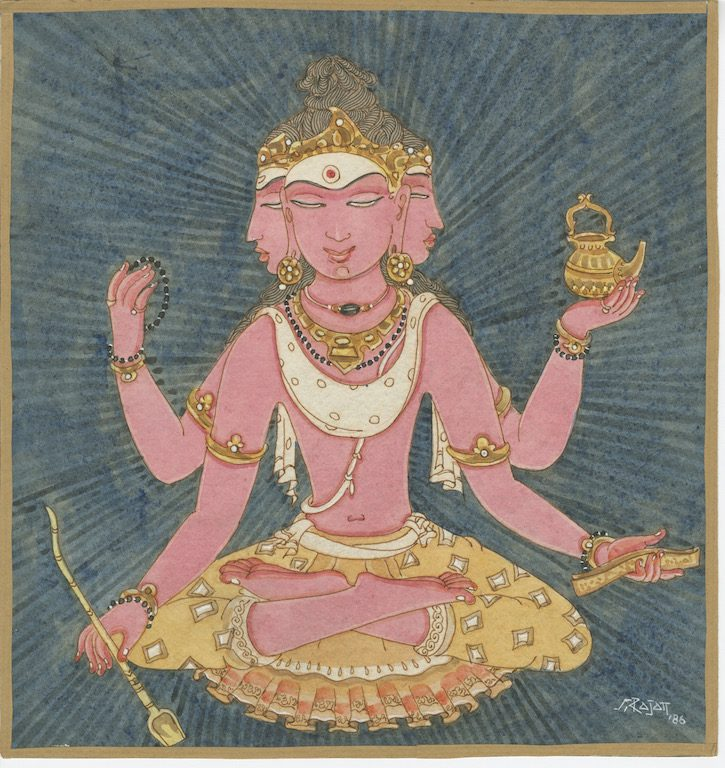
\includegraphics[width=0.5\textwidth]{pics/Brahma.png}
\caption{ Lord Brahma}
 \end{figure}

 

\begin{enumerate}

\item[ ] 1. Brahma or Prajapati, the cosmic creator. This tithi is good for initiating all ventures and for all sacraments and spiritual actions. It is particularly good for planning things, but not so much for actually starting or doing things. The new Moon still casts a shadow on this day.

Prajapati is also the ruler of Rohini (mid-Taurus), the most favorable of the Nakshatras. This tithi, like Rohini, is very good for promoting all positive actions in the initial phase of things. On this tithi one should set forth ones plans for the month.

 

\item[ ] 2. Vidhatar, the cosmic ordainer. This deity is like Brahma but more concerned with establishing structure and order. Whereas the first tithi is good for plans, for planting the seeds of things, this tithi is better for establishing the broader scope of our endeavors.

It has an energy similar to Abijit, also ruled by Vidhatar, a very favorable Nakshatra for giving great victory and high achievement.

 

\item[ ] 3. Vishnu, the cosmic preserver. This tithi is thus good for activities that are meant to be enduring. It is good for bringing things to a high level of development and recognition.

It has an energy similar to Shravana (mid-Capricorn), ruled by Vishnu, which is good for communication, public and teaching ventures.

 

\item[ ] 4. Yama, the God of death and discipline. This tithi is thus unfavorable except for harsh actions and self-discipline.

It has an energy similar to Bharani, also ruled by Yama, and brings karmic retribution.

 

\item[ ] 5. The Moon, Soma. This tithi is favorable for most activities, particularly those involving women, the mother and the emotional nature, which relate to the Moon. It is good for preparing or taking herbal medicines and for natural healing therapies of both body and mind. It is favorable for devotional meditation.

It has an energy similar to Mrigashiras (Orion, late Taurus/early Gemini), also ruled by Soma.

 

\item[ ] 6. Agni, Fire or Skanda, the War God

Ruled by fire, this tithi is good for harsh or fiery actions: Surgery, overcoming enemies, disciplining our physical nature or organizing our material resources.

It has an energy similar to Krittika (the Pleiades, early Taurus), also ruled by Agni.

 

\item[ ] 7. Indra: Deity of Self-power and Transcendence

This tithi is good for actions aimed at establishing independence, for personal gains and for self-development. It can give great success but requires will and motivation.

It has an energy similar to Jyeshta (late Scorpio), ruled by Indra, but is more favorable.

 

\item[ ] 8. The Vasus: Gods of Splendor

It has an energy similar to Dhanishta, ruled by the Vasus. It gives success and splendor but with a tendency toward excess, overdevelopment and diffusion of energies.

 

\item[ ] 9. The Serpent

It has an energy similar to Uttara Bhadra ruled by Ahir Budhnya and hence is to be avoided. It also inclines toward excess and possible deception.

 

\item[ ] 10. Dharma or Brihaspati, God of Religion and Truth

This tithi is favorable for all dharmic and spiritual actions, for rituals, meditation, and for all sacraments and positive actions in life.

It has an energy similar to Pushya (mid-Cancer), also ruled by Brihaspati, which gives the ability to promote all positive ventures.

 

\item[ ] 11. Rudra or Shiva, Deity of Destruction

This tithi is very strong and can give success and transformation but its energy can be difficult to deal with, like the fierce God Rudra. It has an energy similar to Ardra (mid-Gemini), also ruled by Rudra. Yet it is also used for the worship of Vishnu.

 

\item[ ] 12. The Sun (Aditya or Savitar):

This tithi is very auspicious for creative and spiritual actions, particularly for creative work and learning.

It has an energy similar to Hasta (mid-Virgo), also ruled by Savitar.

 

\item[ ] 13. God of Love and Charm (Bhaga):
This tithi is favorable for matters of pleasure, enjoyment, recreation, friendship, social gains, charm, charisma and dealing with the mass media.

It has an energy similar to Purva Phalguni (mid-Leo), also ruled by Bhaga.

 

\item[ ] 14. Strife

This tithi causes conflict and misunderstanding. It is only good for harsh actions like administering drugs or performing surgery, or for black magic.

It has an energy similar to Ashlesha (late Cancer), which can give deception.

 

\item[ ] 15. Full Moon: Universal Gods (Vishve Devas)

This tithi is good for worshipping the Divine, for cosmic action and for promoting the future.

It has an energy similar to Uttarashadha (late Sagittarius), ruled by the Universal Gods.

 

\item[ ] 15. New Moon – the Ancestors

This tithi is good for worshipping the Ancestors, or dealing with ones past.

It has an energy similar to Magha (early Leo), ruled by the Ancestors. It is better for self-examination and for clearing up the past.

The first half of the lunar month is better for spiritual actions and for initiating new activities. The second half is better for personal, social or family matters and for finishing off actions already started.

 

\subsubsection{TITHIS AND PLANETARY ASPECTS}

Each tithi covers 12 degrees of arc between the Sun and Moon. The purna tithis roughly parallel 60, 120 and 180 degree aspects between the Sun or Moon, or trines, benefic aspects in Western astrology. The rikta tithis roughly parallel 45º, 90º and 135º or square and semi-square aspects, malefic aspects in Western astrology.

 

\subsubsection{III. THE DAYS OF THE WEEK}
 

Each day of the week has its characteristic quality based upon the nature of the planet that rules it. Again we must note that the Vedic day begins at sunrise. The nature of the day is the easiest factor to consider, as it requires neither an ephemeris nor a Panchanga. It is usually the first factor that we should consider, and the basis for determining the Nakshatra and Tithi. If we choose an auspicious day for our actions, we have already taken a significant step in protecting them.

 

\subsubsubsection{BENEFIC AND MALEFIC DAYS}

\paragraph{}Days ruled by benefic planets – Monday, Wednesday, Thursday and Friday – Moon, Mercury, Jupiter and Venus – are good for most actions. 
\paragraph{}Thursday and Friday are the best, as Jupiter and Venus are the most auspicious planets.
\paragraph{}Days ruled by malefic planets – Sunday, Tuesday and Saturday – Sun, Mars, and Saturn – have some unfavorability. 
\paragraph{}Tuesday and Saturday are worse in this respect, as their lords are most malefic.


\subsubsubsection{INDICATIONS OF DAYS OF THE WEEK}
 

SUNDAY

Favorable for rituals, meditation, self-knowledge, gains in career or status, receiving honors, honoring tradition, authorities, parents or gurus, worship of the Divine Father (Shiva or Vishnu). Unfavorable for marriage, sexual activity or conception. Not generally useful for business ventures. Not a good day for outward expansion as much as inner examination and for establishing personal intentions and goals to be realized during the week.

 

MONDAY

Favorable for affairs relating to the public or society, for gaining popularity, for relating to women or to the mother, including worship of the Divine Mother, for friends, family and household matters in general. It is good for marriage, sexual activity and conception of children, medical treatment (the Moon is a nurse), rituals, particularly of a devotional nature, and for contemplation and meditation. Can bring financial or business gains through friends and social contact.

 

TUESDAY

Good for physical activity, sports and competitive ventures (but care must be taken not to act recklessly). It is important that we use the restless Mars energy of this day and do not allow it to become bottled up inside ourselves. It is good for developing a warrior energy, and for worshipping Lord Skanda, the Divine warrior (or Rudra, the wrathful form of Shiva, and Candi or Durga, the wrathful form of the Goddess). Also useful for mechanical work, fixing things, for research, mathematical studies, and scientific pursuits.

Tuesday is more favorable in the afternoon than in the morning. Unfavorable for marriage or sexual activity. Generally not good for travel, for legal affairs, for relationship and human issues requiring tact or sensitivity.

 

WEDNESDAY

Good for talking, writing, learning, study, teaching, educational activities, meditation and the development of discrimination. Good for business, commerce, and career gains, communication ventures, making money, marriage and sexual activity. Good for all healing practices, particularly using herbs, and the making of medicines. Also good for healing the mind and all psychological studies. A good day for the worship of Lord Vishnu. Yet more a day for creating the theoretical background for our projects than for trying to initiate anything lasting.

 

THURSDAY

The most favorable day of the week generally for all good actions, including religious rituals, ceremonies, meditation, study and worship of the Divine, the guru or traditions. Good for financial gain, speculative ventures, career advancement, and for enjoyment and social interaction. Good for healing practices in general, exercise of all types, reconciliation, and for giving gifts. Excellent for legal matters. Favorable for marriage, sexual activity, or conception of children. Also good for the affairs of children. The best day for initiating expansive ventures that we hope will endure. Good for worshipping Lord Ganesha.

 

FRIDAY

Good for artistic ventures, decorations and ornaments, business ventures, purchasing vehicles, buying gems, clothes, or other precious items, for affairs relative to women (marriage, sexual activity, romance), enjoyment and entertainment. Also good for devotional practices or study of the occult, particularly for the worship of the Divine Mother, especially in her blissful form (Lalita).

 

SATURDAY

Unfavorable for most social or business matters, as it usually brings loss or opposition, but good for acquiring fixed property and for doing service work. Not good for health, marriage, or for sexual activity, but good for retreat, study, meditation and relaxation. Also good for self-discipline, yoga, fasting and ascetic practices. A good day to spend time alone. Good for worshipping the dark or wrathful forms of the Divine, like the terrible forms of Shiva (like Bhairava) and his consort (like Kali).

Our cultural tendency is to escape the influence of Saturn on Saturday by turning it into a day of self-indulgence but this is not wise, as it keeps our lives out of the control of our deeper nature and spiritual intent. Hence, Saturday is perhaps the most important day of the week for structuring our time wisely.

 

\subsubsection{NOTES ON THE DAYS}

 

We must remember that these are only general indications. The position of the planet on that day must be considered as well. For example, if Mercury is with Saturn and Rahu, Wednesday may cause loss and difficulties with communication and business.

 

The effects of the days of the week on an individuals life varies according to the place and strength of the planet within the individuals birth chart. For example, if a person has a strong Mars as a Raja Yoga Karaka, Tuesday would be very favorable for work, career, or starting new ventures.

 

\subsubsection{COMBINING THE DAY, TITHI AND NAKSHATRA}

It is best to combine favorable days, Tithis and Nakshatras for the best possible results. When a favorable day of the week, like Thursday or Friday, is under a favorable Tithi, like the fifth or the tenth, it is a good day for auspicious actions. If, in addition, the Moon is in a favorable Nakshatra – like Pushya, Punarvasu, Rohini, Mrigashiras, Revati, Uttara Phalguni, Uttara Bhadra or Chitra – then the results are quite excellent.

 

When such a good day is under a favorable Tithi for meditation, like the ninth, fourteenth or fifteenth, then it becomes very strong for that. If, in addition, the Moon is in a Nakshatra favorable for worship, which varies relative to the type of deity or the type of worship involved, the results will also be favorable.

 

\subsection{IV. KARANAS}


Each Tithi is divided into two Karanas. Karana means “instrument”. The Karanas help give us the means to fulfill our actions. These are named according to different animals. In total there are eleven Karanas.

 

\subsubsection{KARANAS}

 
\begin{center}
\begin{tabular}{ l l l}
1.  LION (Bava)&	2,  9, 16, 23, 30, 37, 45, 51             \\
2.  LEOPARD (Balava)	&3, 10, 17, 24, 31, 38, 46, 52            \\
1.    PIG (Kaulava)	&4, 11, 18, 25, 32, 39, 47, 53            \\
2.    DONKEY (Taitula)	&5, 12, 19, 26, 33, 40, 48, 54            \\
3.    ELEPHANT (Garija)	&6, 13, 20, 27, 34, 41, 49, 55            \\
4.    COW (Vanija)	&7, 14, 21, 28, 35, 42, 50, 56            \\
5.    VISHTI	&8, 15, 22, 29, 36, 43, 51, 57            \\
6.    PULLU (Shakuna)	&58            \\
7.    CATTLE (Chatuspada)	&59            \\
8.    SNAKE (Naga)	&60            \\
9.    WORM (Kimstughna)	&1            \\
\end{tabular}
\end{center}

 
\begin{enumerate}

\item[*] The first one and last three Karanas are fixed in nature. They relate to the time of the new Moon and show the enduring factor of the Moons power.

 

\item[*] The remaining fifty-six Karanas are said to be mutable in nature. They show the fluctuations of the lunar force.

 

\item[*] The fixed Karanas and the Vishti Karanas are considered to be generally unfavorable in nature and actions should not be done during them.

 

\item[*] The fixed Karanas occur during unfavorable Tithis anyway and are generally rejected on that account. They relate to the latter half of the fourteenth day of the waning Moon, the day of the new Moon, and the first half of the day after the new Moon. Hence, the first half of the first day of the waxing Moon is more unfavorable than the second half. By this system, we can understand why the new Moon, though technically a Purna or full Tithi, is unfavorable. Both of its Karanas are negative.

 

\item[*] The Fixed Karanas (58, 59, 60, 1) and, of the Mutable class, those of the Vishti group (8, 15, 22, 29, 36, 43, 50, 57) are considered to be generally unfavourable and inauspicious in nature, therefore, the performance of any kind of action should be avoided under them.

 

\item[*] The Fixed Karanas, occurring once a (lunar) month as a transition between the two halves (Pakshas) of the Moon, cover a two-day time period, in lunar terms, (four consecutive half-days, or two Tithis).

 

\item[*] For the remaining period of time, the Karanas of Vishti (and of the other groups) occur in alternation eight times each in a (lunar) month, on every seventh (lunar) half-day (8 x 7 = 56).

 

\item[*] Vishti Karana occurs in the bright half of the Moon in the first half of the 4th Tithi (which is generally rejected as unfavorable anyway), the first half of the 8th Tithi (also generally rejected), the second half of the 11th Tithi, and the first half of the full Moon Tithi. During the dark half of the Moon, it occurs on the second half of the 3rd Tithi, the first half of the 7th Tithi, the second half of the 10th Tithi, and the first half of the 14th Tithi (also generally rejected).

 

\item[*] The Karanas of the lion are good for starting ventures of an enduring nature, those of the donkey are good for marriage.

 \end{enumerate}

\subsubsection{INDICATIONS OF KARANAS}

 

Below are some typical classical indications of the Karanas mainly for birth but also for action. They are delineated briefly, as in themselves they are not that important.

 
\begin{center}
\begin{tabular}{ l l l}
1. BAVA	&Youthful, childish, valiant                         \\
2. BALAVA	&Modest, careful in conduct, respected                        \\
3. KAULAVA	&Impressive, active, dramatic                        \\
4. TAITULA	&Skillful in speech and action, able to influence                        \\
5. GARIJA	&Powerful, able to overcome opposition                        \\
6. VARIJA	&Clever, passionate, may be lacking in self-control                        \\
7. VISHTI	&Gives opposition, acts contrary to normal order, culpable, self-reliant, honored by his followers                        \\
8. SHAKUNA	&Able to read events, psychic perception, intelligence, prosperity                        \\
9. CHATUSPADA	&Many obstacles, yet many possibilities, comprehensive                        \\
10. NAGA	&Ambitious, powerful, dangerous                        \\
11. KIMSTUGHNA	&Dependent, changeable, superficial, easy going                        \\
\end{tabular}
\end{center}
 

 

\subsection{V. PANCHANGA YOGAS}
 

The term Yoga has several usages in Vedic Astrology. Here it is used relative to Muhurta or Electional Astrology. Like the Nakshatras, each Yoga relates to a 13º 20 section of the zodiac. Yet it is calculated differently. Below we present how to calculate the Yogas. This material, however, is not important to memorize, as most of the time we will merely look the Yogas up in the almanac.

 
\begin{enumerate} 
\item[] To calculate the Yoga, add the longitudes of the Sun and the Moon and divide the amount by 800 (the number of minutes in 13°20).

 

\item[] For example, if the Moon is at 14° 20 Gemini, its longitude from the point 0 Aries would be 74° 20. If the Sun is at 20° 40 Sagittarius, its longitude would be 260° 30.

 

\item[] Adding these together, 74°20 plus 260°40 we would get 334° 50. If we get a number higher than 360, we should subtract 360 from it.

 

\item[] This we then turn into minutes by multiplying the degrees by 60, which would be 20,040 plus 50 for the minutes or 20,090.

 

\item[] We then divide this amount by 800, which gives us 25.1125. This places us in the twenty-sixth yoga – Brahma yoga – as the twenty-fifth has already finished.

 

\item[] To determine when a particular yoga ends, multiply the remainder by 24. In the above example 24 x .1125 is 2.7 or two houses and forty-two minutes from the particular time in question.

 \end{enumerate}

\subsubsection{INDICATIONS OF YOGAS}
 

Below are typical indications of Yogas both for birth charts and for the purposes of astrological forecasting.

 
\begin{center}
\begin{tabular}{ l l l}
1.    VISHKAMBHA*	&Overcomes obstacles, gains wealth and property                                \\
2.    PRITI*	&Easily influenced by attractive objects                               \\
3.    AYUSHMAN	&Good for health and longevity                               \\
4.    SAUBHAGYA	&Gives happiness, is auspicious for action                               \\
5.    SOBHANA	&Gives beauty but also sensuality                               \\
6.    ATIGANDA*	&Destructive and deceptive tendency, clever                               \\
7.    SUKARMA	&Good for action, work and accomplishment                               \\
8.    DHRITI*	&Dominates and controls other people                               \\
9.    SHULA*	&Gives anger, conflict and pain                               \\
10. GANDA*	&Gives attachments and addictions                               \\
11. VRIDDHI	&Gives wisdom, speech capacity and increase                               \\
12. DHRUVA	&Gives stability, firmness and wealth                               \\
13. VYAGHATA*	&Dangerous and wrathful, can bring injury                               \\
14. HARSHANA	&Exhilarating, gives joy, fame and wisdom                               \\
15. VAJRA*	&Gives will, power, energy and motivation                               \\
16. SIDDHI	&Gives success and protection                               \\
17. VYATIPATHA*	&Deceptive, unclear, moving in many directions                               \\
18. VARIYAN*	&Causes one to seek gain, can give greed, ambition                               \\
19. PARIGHA*	&Inimical but wealthy and successful                               \\
20. SHIVA 	&Auspicious, peaceful, intelligent, loved                               \\
21. SIDDHA	&Successful, virtuous, adept, skillful                               \\
22. SADHYA	&Righteous (virtuous), able to accomplish goals                               \\
23. SHUBHA	&Gives beauty and wealth but may give sensuality                               \\
24. SHUKLA	&Gives intelligence, powers of speech, is virtuous but changeable in mind and difficult to please                               \\
25. BRAHMA	&Gives wisdom, good judgment, honor, secret wealth                               \\
26. AINDRA	&Gives comprehensive intellect, beneficence, wealth, power, honor, prestige                               \\
27. VAIDHRITI*	&Firm, powerful, wealthy but obstinate and inflexible                               \\
\end{tabular}
\end{center}
 

*less favorable

 

\begin{enumerate} 
\item[] Of these Yogas, the first, sixth, ninth, tenth, fifteenth, seventeenth and twenty-seventh are inauspicious.
\item[] The twenty-first, twenty-fifth and twenty-sixth are particularly auspicious.
\item[] All other remaining Yogas are considered favourable, particularly 21 (Siddha), 25 (Brahma), and 26 (Aindra), under which all auspicious undertakings are permitted.
 

Main  Inauspicious  Yogas

 
\begin{center}
\begin{tabular}{ l l l}
Yoga	Sanskrit  &Name	Meaning	&Time  Period  To  Be  Avoided                               \\
1	Vishkambha	&Pot filled with poison	&First 3 Ghatis (1 hour  and 12 minutes)                               \\
6	Ati-Ganda	&Very strong knot (obstacle)	&First 6 Ghatis (2 hours and 24 minutes)                               \\
9	Shula	&Sharp or pointed weapon	&First 5 Ghatis (2 hours)                               \\
10	Ganda	&Knot (hindrance)	&First 6 Ghatis (2 hours and 24 minutes)                               \\
13	Vyaghata	&Striking against (obstacle)	&First 9 Ghatis (3 hours and 36 minutes)                               \\
15	Vajra	Thunderbolt, lightening	&First 3 Ghatis (1 hour  and 12 minutes)                               \\
17	Vyatipata	&Destruction	 &60 Ghatis (Whole time period)                               \\
19	Parigha	&Iron bar / club	&30 Ghatis (First half of Yoga)                               \\
27	Vaidhriti	&Division	&60 Ghatis (Whole time period)                               \\
 \end{tabular}
\end{center}

\subsubsection{USING KARANA AND YOGA}

Once we have determined a favorable Day, Tithi and Nakshatra, we should check to see if an unfavorable Yoga and Karana are in existence that could cause obstruction. If this is not the case, the outcome becomes more favorable. If it is the case, we may look to a part of the day when the negative Yogas and Karanas are not in operation, or we can look to another favorable day, Tithi and Nakshatra that do not have such a negative condition.

 

There is a part of this system which delineates specific Tithis coinciding with particular days of the week as being auspicious or inauspicious. Certain combinations of weekdays and lunar days, Varas and Tithis, give rise to certain qualities during the time period in question, according to the integration of the individual qualities of these two time factors.

 

Siddha Tithi  (Auspicious Tithis)

 
\begin{center}
\begin{tabular}{ l l l}
Tithi  Group	&Tithis	&Vara                                     \\
Nanda	&1,  6,  11&	Friday                              \\
Bhadra	&2,  7,  12	&Wednesday                              \\
Jaya	&3,  8,  13	&Tuesday                              \\
Rikta&	4,  9,  14	&Saturday                              \\
Purna	&5, 10, 15	&Thursday                              \\
 \end{tabular}
\end{center}

Dagdha Tithi  (Inauspicious Tithis)

 
\begin{center}
\begin{tabular}{ l l l}
Tithi  Group	&Vara                              \\
Nanda	&Sunday, Tuesday                              \\

Bhadra	&Monday, Friday                              \\

Jaya	&Wednesday                              \\
Rikta	&Thursday                              \\
Purna	&Saturday                              \\
  \end{tabular}
\end{center}

Krakacha  Tithi  (Inauspicious Tithis)

(Tithi + Vara = 13)

 
\begin{center}
\begin{tabular}{ l l l}
Tithi	&Vara \\
12 Dwadashi	&1 Sunday                             \\
11 Ekadashi	&2 Monday                             \\
10 Dashami	&3 Tuesday                             \\
  9 Navami	&4 Wednesday                             \\
  8 Ashtami	&5 Thursday                             \\
  7 Saptami	&6 Friday                             \\
  6 Shashti	&7 Saturday                             \\
   \end{tabular}
\end{center}

 
\subsubsection{ADDITIONAL FACTORS BEYOND THE PRIMARY FIVE}
 

There are several additional factors to consider beyond the usual five of the Panchanga, which overlap with them to some degree.

 

\subsubsection{ADDITIONAL FACTORS RELATIVE TO THE SUN}
 

There are some incidental factors relative to the Sun that should be considered for the timing of actions.

 

\subsubsection{THE SUN’S MOVEMENT INTO NEW SIGNS – SANKRANTI}

The Sun’s movement into new signs of the zodiac, called Sankranti, is also a time period that is not favorable for actions. It is similar to the Western idea of the Moon being void of course and hence unfavorable when it crosses between signs. It is mainly the period of about six hours before and after changing signs that is inauspicious, the last fifteen minutes or quarter of a degree of one sign and the first fifteen minutes of another.

 

When other planets are in the last or first degree of a sign, this can also cause difficulties.

 

\subsubsection{EQUINOCTIAL AND SOLSTICE POINTS}

The days of the equinoxes and solstices are additional important transitional periods. Hence, they are more favorable for rituals and meditation than for ordinary activities. Most important perhaps is the day of the winter solstice as it allows us to bring in a spiritual energy for the whole year.

 

Like transitional points of sunrise and sunset, the solstices and equinoxes are points at which the mind can more easily become still and the Prana or vital energy can enter the central channel for inner transformation. Hence, these times are important for spiritual rather than ordinary actions.

 

\subsubsection{THE NORTHERN AND SOUTHERN COURSES OF THE SUN}

Actions are best done during the northern course of the Sun (Uttarayana), the period between the winter and the summer solstices (December 22—June 21). This is the best time for such things as marriages, initiations, or even for death (it is best to die at the winter solstice according to Vedic thought).

 

For actions done in the southern course of the Sun, they are best if done during the bright half of the Moon.

 

The northern course of the Sun, as we noted in the section of the course on chakras, relates to the movement of the Prana up the spine. Hence, it is also better for spiritual practices.

 

\subsubsection{ECLIPSES}

Eclipses are important points of energy transformation, and perhaps the most important transitional periods of all. They bring the energy into the central channel and allow the mind to be still, withdrawing it from its ordinary outward actions. Hence, they are also very favorable for rituals and meditation but not for ordinary activities.

 

Lunar eclipses are important times for purification and negation of the mind. Solar eclipses are important times for self-knowledge and transcendence of the ego.

 

\subsubsection{GANDANTA MOON}
The Moon located in the first navamsha (3º 20) of fire signs or the last quarter of water signs is inauspicous for actions and dangerous for the birth of children. This position is the first quarter of Ashwini, Magha and Mula Nakshatras and the last of Revati, Aslesha and Jyeshta Nakshatras.

 

Jyeshta-Mula or Scorpio-Sagittarius Gandanta is considered to be the worst. Aslesha-Magha or Cancer-Leo Gandanta is second. Revati-Ashwini or Pisces-Aries is not always so bad.

 

The same positions are difficult for other planets but only in the first and last degrees of the respective signs, not through the entire 3º 20 section. The full Gandanta arc of 3º 20 applies only to the Moon as it is a fast-moving planet.

 

\subsubsection{LUNAR MONTHS}
In India, a lunar calendar is employed from new Moon to new Moon, named after the Nakshatra in which the Moon becomes full in during the month. The twelve Hindu months are:

 
\begin{center}
\begin{tabular}{ l l l}
Ashwin – October	&Karttika – November                              \\
Margashirsa – December	&Pushya – January                             \\
Magha – February	&Phalguni – March                             \\
Caitra – April	&Vaishakha – May                             \\
Jyeshta – June	&Ashadha – July                             \\
Shravana – August	&Bhadrapada – September                             \\
   \end{tabular}
\end{center} 

As these months depend upon the Moon, they vary slightly every year and hence their equivalence to various Western months is very approximate. Again, an almanac is needed for determining them. Every 2½ years an additional or intercalary month has been added, as the lunar year of twelve months falls eleven days short of the solar year of 365 days.

 

The different lunar months have their own characteristics and importance. Various days within them relate to holy days among the Hindus and Buddhists. This matter has its complexity and it is our intention only to introduce it here.

 

Generally, the months comprising the northern course of the Sun (Margashirsha to Jyeshta) are better than those under the southern course (Ashadha to Karttika).

 

The month of Magha is generally not favorable for putting on gems, installing altars or forms of deities, or other religious and spiritual issues. The months of Karttika and Mrigashiras are particularly favorable for spiritual practices and rituals. Different Hindu and Buddhist deities have their special days in different months, like Shiva Ratri in February, the nine days of Durga in October, the sacred day of the Buddha in Vaishakha, or the birth day of Krishna in August. These are regulated according to the lunar calendar.

However, the months are a secondary consideration, as many actions must be performed every month.

 

\subsubsection{THE PLACE OF ASTROLOGICAL FORECASTING}

Naturally, we dont always have the time to examine all such astrological factors in detail before initiating all actions, and astrology cannot substitute for our own power of judgment. In the modern world, we cannot always modify these factors either. For example, we cannot always get airplane tickets at the most auspicious times for travel. And, just because a day is favorable for accumulating wealth does not mean that it is right for us to do so. We must always look back to the dharma of the person to determine which of these favorable potentials is best for them. In this regard, it is more important that we do what is best for us, rather than do what is best for the particular day involved, though it is ideal to be able to combine both together to some degree. If we focus on the spiritual life, for example, many of these outer potentials lose their attraction for us.

 

As an astrologer, astrological forecasting may not be our primary interest but we should at least be acquainted with the subject or we cannot be said to be truly aware of the complete scope of Vedic Astrology.

 

For further study, we recommend the Kala Prakashika, translation by N.P. Subramania Iyer. Yet we should note that, owing to changes in time and culture, the whole system of Astrological Forecasting requires perhaps more readjustment than the reading of birth charts. Much of the traditional information on the subject, reflecting the customs of medieval India, may not be of relevance for us today.

 


\subsubsection{SUPPLEMENT
LUNAR MONTHS AND SACRED TITHIS OF THE HINDU CALENDAR}
 

The following days are good for various planets and various actions even apart from the usual Tithi and Nakshatra indications. As these lunar months vary every year, you must check the yearly Panchanga to find out which exact days of the Western solar calendar they correspond to. Actions done on special days are much more powerful. This extends to astrological remedial measures.

(Key:  * sacred days    ** days good for all actions, Shukla is waxing Moon, Krishna or K. is waning Moon, month indications begin with waxing Moon)

 

Chaitra – April

 
\begin{enumerate} 
\item[] **Pratipat – Astronomical new year  — all
\item[] Panchami – Matsya  Jayanti — Ketu
\item[] Ashtami – Durga — Rahu
\item[] *Navami – Rama Jayanti — Sun
\item[] Trayodashi – Mahavira (Jaina) Jayanti
\item[] Purnima – Chitragupta/Hanuman Jayanti — Ketu, Mars
\item[] K. Ashtami – Sitala Devi, to counter fevers and diseases — Ketu, Mars
\end{enumerate}
 

Vaishakha – May
\begin{enumerate} 
\item[] **Tritiya – Parshurama Jayanti, Akshayya (Satya Yuga) — all, Venus
\item[] Panchami – Shankaracharya Jayanti
\item[] Saptami – Ganga Devi — Mercury
\item[] Chaturdashi – Nrisimha Jayanti — Mars
\item[] *Purnima – Buddha Purnima, Kurma jayanti — Mercury, Saturn
 \end{enumerate}

Jyeshta – June
\begin{enumerate} 
\item[] Purnima – Savitri, Snana Yatra of Ratha Yatra — Sun
\item[] K. Caturdasha – Savitri
 \end{enumerate}

Ashadha – July
\begin{enumerate} 
\item[] Dvitiya – Rathayatra, Jagannath Puri — Sun
\item[] *Shasti – Skandha — Mars
\item[] Ashtami – Durga Shayana
\item[] Ekadashi – Vishnu Shayana
\item[] *Purnima – Guru Purnima, Vyasa — Jupiter, Mercury
\item[] Shravana – August
\item[] Panchami – Naga Panchami — Rahu, Ketu
\item[] Saptami – TulsiDasha Jayanti
\item[] *Ashtami – Krishna Janmashatami — Moon
\item[] *Purnima – Raksha Bandhana — all malefics
\item[] K. Chaturthi – Ganesha
 \end{enumerate}

Bhadrapada – September
\begin{enumerate} 
\item[] Dvitiya – Balarama Jayanti
\item[] Tritiya – Varaha jayanti
\item[] *Chaturthi – Ganesh Chaturthi – noon — all planets, Jupiter, Ketu
\item[] Panchami – Rishi Panchami — Mercury, Jupiter, Ketu
\item[] Ashtami – Indra Dvaja / Radha Jayanti — Jupiter, Venus
\item[] Dvadashi – Vamana jayanti — Jupiter
\item[] Chaturdashi – Ananta — Rahu, Ketu
\item[] Purnima – Uma Maheshvara Vrata — Sun, Moon
\item[] Krishna  Paksha – Pitripaksha
\item[] K. Trayodashi – Dwapara Yugadi
\item[] Amavasya – Mahalaya — Saturn
 \end{enumerate}

Ashvina – October
\begin{enumerate} 
\item[] Navaratri (nine day festival)
\item[] *Pratipat, *Dvitiya, *Tritiya, *Chaturthi, *Panchami
\item[] *Shashti – Durga Bodhana
\item[] *Saptami – Saraswati — Mercury
\item[] *Ashtami – Durga — Rahu
\item[] *Navami
\item[] **Dashami – Vijay Dashami — Moon, Venus
\item[] Purnima – Sharat Purnima, Lakshmi — Moon, Venus
\item[] K. Trayodashi – Dhanvantari — Mercury
\item[] *K. Caturdashi – Dipavali 1- Naraka Chaturdashi, Kali, Hanuman — Saturn
\item[] *Amavasya – Lakshmi — Moon, Venus
 \end{enumerate}

Karttika – November
\begin{enumerate} 
\item[] **Pratipad – Dipavali, Balipratipat, Bali Puja, religious new year — All
\item[] *Dvitiya – Dipavali, Yama/Yamuna, Vishvakarma
\item[] Shasti – Skanda, Surya – Mars, Sun
\item[] Saptami – Sun
\item[] Navami – Treta Yugadi
\item[] Ekadashi – Vishnu Prabodhini — Mercury, Sun
\item[] Dvadashi – Vishnu Utthana, Tulasi Devi
\item[] Chaturdashi – Vaikuntha Chaturdashi Vrata
\item[] *Purnima – Dipam, Shiva, Skanda — Mars
\item[] K. Ashtami – Bhairavi
\item[] Amavasya – Durga, Kali — Rahu, Saturn
 \end{enumerate}

Margashirsha – December
\begin{enumerate} 
\item[] Chaturthi – Ganapati-Varada — all planets, Jupiter
\item[] *Panchami – Sri/Lakshmi — Moon, Venus
\item[] Shasti – Skanda — Mars
\item[] Ekadashi – Vaikuntha, Gita Pravachana, Gita Jayanti, Vishnu — Sun, Mercury
\item[] Dvadashi – Vaikuntha, Vishnu
\item[] Purnima – Dattatreya, Nataraja Darshana
 \end{enumerate}

Pushya – January
\begin{enumerate} 
\item[] K. Saptami – Vivekananda Jayanti
 \end{enumerate}

Magha – Februrary
\begin{enumerate} 
\item[] *Panchami – Vasanta – Saraswati — Mercury, Moon
\item[] *Saptami – Ratha Saptami – Surya, Vaivasvata Manvantara — Sun
\item[] Ashtami – Bhishma Mahasamadhi
\item[] Ekadashi – Bhima
\item[] Purnima – Snana – Sun
\item[] *K. Chaturdashi – Shiva Ratri — Saturn
\item[] Amavasya – Muni Amavasya/ Kali Yugadi, Mahamela — Saturn
 \end{enumerate}

Phalguna – March
\begin{enumerate} 
\item[] Dvitiya – Ramakrishna Jayanti
\item[] Ashatmi – Sita Jayanti — Venus
\item[] Ekadashi – Amalaki Vrata
\item[] *Purnima – Holi, Prahlada — Venus
\end{enumerate}

All Months
\begin{enumerate} 
\item[] Pratipad, Shukla – For all spiritual actions and initiation
\item[] Chaturthi, particularly Shukla – Ganesh — Jupiter, Ketu
\item[] Panchami, Shulka – The Goddess in her benefic forms, Lakshmi, Saraswati — Moon, Venus
\item[] Shasti, particularly Shukla – Skanda — Mars
\item[] Ashtami, Shukla – Devi – Moon, Venus, Rahu
\item[] Dashami, Shukla – Good for all planets
\item[] Ekadashi – Vishnu, particularly Shukla — Sun, Mercury, Also good for fasting
\item[] Trayodashi, Shukla — Pradosha, Shiva
\item[] Purnima – For meditation
\item[] K. Chaturdashi – Shiva, Kali, Masa Amavasya — Saturn
 \end{enumerate}

Other Important Dates
\begin{enumerate} 
\item[] Also Sankrantis or Sun changing signs, particularly Capricorn and Cancer
\item[] Solstices, equinoxes, and eclipses
\end{enumerate}
\newpage




% ------------------------------------------------------------------------------

\end{document}
